\documentclass{article}


% if you need to pass options to natbib, use, e.g.:
\PassOptionsToPackage{numbers, sort, compress}{natbib}
%\usepackage[numbers,sort&compress]{natbib}
% before loading neurips_2023


% ready for submission
% \usepackage{neurips_2023}


% to compile a preprint version, e.g., for submission to arXiv, add add the
% [preprint] option:
% \usepackage[preprint]{neurips_2023}


% to compile a camera-ready version, add the [final] option, e.g.:
\usepackage[final]{neurips_2023}


% to avoid loading the natbib package, add option nonatbib:
%    \usepackage[nonatbib]{neurips_2023}


\usepackage[utf8]{inputenc} % allow utf-8 input
\usepackage[T1]{fontenc}    % use 8-bit T1 fonts
\usepackage[colorlinks=true, citecolor=blue, linkcolor=black, urlcolor=Violet]{hyperref}       % hyperlinks
%\usepackage{hyperref}
\usepackage{url}            % simple URL typesetting
\usepackage{booktabs}       % professional-quality tables
\usepackage{amsfonts}       % blackboard math symbols
\usepackage{nicefrac}       % compact symbols for 1/2, etc.
\usepackage{microtype}      % microtypography
\usepackage[dvipsnames]{xcolor}         % colors
\usepackage{subfigure}
\usepackage{multirow}
\usepackage{multicol} 
\usepackage{pifont}
\usepackage{graphicx}
\usepackage{algorithm}
\usepackage{algorithmic}
\usepackage{caption}
\usepackage{amsmath}
\usepackage{amssymb}
\usepackage[font={footnotesize}]{caption}


\usepackage[utf8]{inputenc} % allow utf-8 input
\usepackage[T1]{fontenc}    % use 8-bit T1 fonts
\usepackage{hyperref}       % hyperlinks
\usepackage{url}            % simple URL typesetting
\usepackage{booktabs}       % professional-quality tables
\usepackage{amsfonts}       % blackboard math symbols
\usepackage{nicefrac}       % compact symbols for 1/2, etc.
\usepackage{microtype}      % microtypography
%\usepackage{xcolor}         % colors
% \usepackage[table]{xcolor}
% \usepackage{tcolorbox}

 
 \usepackage{graphicx}
\usepackage{subfigure} 
\usepackage{pifont}
%%%%%%%%%%%%%%%% Customized by SL
% \input{math_commands.tex}
\usepackage{adjustbox}
\usepackage{lipsum}
\usepackage{color}
\usepackage{wrapfig}
\usepackage{booktabs}
\usepackage[textsize=scriptsize]{todonotes}
\usepackage{multirow,mathtools}
% \usepackage{algorithm,algpseudocode}
\usepackage{threeparttable}
%\usepackage{xcolor}
% \usepackage[dvipsnames]{xcolor}


%  \algnewcommand{\algorithmicforeach}{\textbf{for each}}
% \algdef{SE}[FOR]{ForEach}{EndForEach}[1]
%   {\algorithmicforeach\ #1\ \algorithmicdo}% \ForEach{#1}
%   {\algorithmicend\ \algorithmicforeach}% \EndForEach
  
  
\definecolor{lightblue}{rgb}{0.68, 0.85, 0.9}
\definecolor{lightgreen}{rgb}{0.56, 0.93, 0.56}
\definecolor{lightskyblue}{rgb}{0.53, 0.81, 0.98}
\definecolor{non-photoblue}{rgb}{0.64, 0.87, 0.93}
\definecolor{magicmint}{rgb}{0.67, 0.94, 0.82}
\definecolor{mossgreen}{rgb}{0.68, 0.87, 0.68}
\definecolor{salmon}{rgb}{1.0, 0.55, 0.41}
\definecolor{babypink}{rgb}{0.96, 0.76, 0.76}
\definecolor{darkgreen}{rgb}{0, 0.7, 0}


\newtheorem{myprop}{\bf{Proposition}}
\newtheorem{mycor}{\bf{Corollary}}
\newtheorem{mythr}{\bf{Theorem}}
\newtheorem{mylemma}{\bf{Lemma}}
\newtheorem{myremark}{\bf{Remark}}
\DeclareMathOperator{\tr}{tr}
\DeclareMathOperator{\card}{card}
\DeclareMathOperator{\cov}{cov}
\DeclareMathOperator{\diag}{diag}
\DeclareMathOperator*{\minimize}{\text{minimize}}
\DeclareMathOperator*{\maximize}{\text{maximize}}
\DeclareMathOperator*{\st}{\text{subject to}}
\DeclareMathAlphabet\mathbfcal{OMS}{cmsy}{b}{n}
\newcommand{\Def}[0]{\mathrel{\mathop:}=}
\newcommand{\Deff}[0]{=\mathrel{\mathop:}}



 \newcommand{\YL}[1]{\textcolor{orange}{YL: #1}}
 
 \newcommand{\SL}[1]{\textcolor{purple}{SL: #1}}
 \newcommand{\JH}[1]{\textcolor{blue}{JH: #1}}
 \newcommand{\JC}[1]{\textcolor{darkgreen}{JC: #1}}
 \newcommand{\PR}[1]{\textcolor{brown}{{\scriptsize [PR: #1]}}}
  \newcommand{\PS}[1]{\textcolor{magenta}{{\scriptsize [PS: #1]}}}
 \newcommand{\revision}[1]{\textcolor{cyan}{revision: #1}}
 
% \def\remark{\addtocounter{remark}{1}\def\@currentlabel{\theremark}%
% \emph{Remark~\theremark}. } \makeatother
% \newcommand{\ubar}[1]{\underaccent{\bar}{#1}}
% \newcommand{\overbar}[1]{\mkern 1.5mu\overline{\mkern-1.5mu#1\mkern-1.5mu}\mkern 1.5mu}
% \newcounter{remark}


\def\balpha{\boldsymbol{\alpha}}
\def\btheta{\boldsymbol{\theta}}
\def\bdelta{\boldsymbol{\delta}}
\def\bbeta{\boldsymbol{\beta}}
\def\bseta{\boldsymbol{\eta}}
\def\bdelta{\boldsymbol{\delta}}




\usepackage{color, colortbl}
\definecolor{Gray}{gray}{0.93}
\definecolor{Orange}{rgb}{1,0.5,0}
\definecolor{DGray}{gray}{0.83}
\definecolor{LightCyan}{rgb}{0.88,1,1}


\usepackage[most]{tcolorbox}
\newtcolorbox{mybox}[2][]{%
  attach boxed title to top center
               = {yshift=-8pt},
  colback      = Gray,
  colframe     = black,
  fonttitle    = \bfseries,
  colbacktitle = white,
  title        = #2,#1,
  enhanced,
}


\DeclarePairedDelimiterX{\inp}[2]{\langle}{\rangle}{#1, #2}


\DeclareMathOperator*{\argmax}{arg\,max}
\DeclareMathOperator*{\argmin}{arg\,min}

\makeatletter
\newcommand*{\rom}[1]{\expandafter\@slowromancap\romannumeral #1@}
\makeatother
\newcommand{\mycomment}[1]{}

\definecolor{Sijia_color}{rgb}{0.858, 0.188, 0.478}
%%%%%%%%Sijia Liu 

\newcommand{\MU}{{\text{MU}}}
\newcommand{\Df}{\mathcal D_\mathrm{f}}
\newcommand{\Dr}{\mathcal D_\mathrm{r}}
\newcommand{\thetaunl}{\boldsymbol \theta_\mathrm{u}}
\newcommand{\thetafull}{\boldsymbol \theta_\mathrm{o}}
\newcommand{\Lunl}{L_\mathrm{u}}


\newcommand{\retrain}{{\text{Retrain}}}
\newcommand{\FT}{{\text{FT}}}
\newcommand{\GA}{{\text{GA}}}
\newcommand{\FF}{{\text{FF}}}
\newcommand{\IU}{{\text{IU}}}


\newcommand{\retrainC}{{\color{red}{\text{Retrain}}}}
\newcommand{\FTC}{{\color{ForestGreen}{\text{FT}}}}
\newcommand{\GAC}{{\color{blue}{\text{GA}}}}
\newcommand{\FFC}{{\color{YellowOrange}{\text{FF}}}}
\newcommand{\IUC}{{\color{purple}{\text{IU}}}}

\newcommand{\UA}{{\text{UA}}}
\newcommand{\RA}{{\text{RA}}}
\newcommand{\TA}{{\text{TA}}}

\newcommand{\MIAF}{{\text{MIA}-Efficacy}}
%\newcommand{\MIAR}{{\text{MIA}-$\Dr$}}
\newcommand{\MIAR}{{\text{MIA}-Privacy}}
\newcommand{\RTE}{{\text{RTE}}}

\newcommand{\thetaEU}{\boldsymbol \theta_\mathrm{\retrain}}

\newcommand{\MUSparse}{{\text{$\ell_1$-sparse MU}}}

\newcommand{\FTSparse}{{\text{$\ell_1$-sparse FT}}}

\newcommand{\acc}{{\text{Acc}}}
\newcommand{\TIME}{{\text{Time}}}



% \newcommand{\MUAO}{{\text{AO-sparse MU}}}

% \newcommand{\FTAO}{{\text{AO-sparse FT}}}
%%%%%%%%%%%%%%%%%%%%%%%%%%%%%%%%
% THEOREMS
%%%%%%%%%%%%%%%%%%%%%%%%%%%%%%%%
% \theoremstyle{plain}
% \newtheorem{theorem}{Theorem}[section]
% \newtheorem{proposition}[theorem]{Proposition}
% \newtheorem{lemma}[theorem]{Lemma}
% \newtheorem{corollary}[theorem]{Corollary}
% \theoremstyle{definition}
% \newtheorem{definition}[theorem]{Definition}
% \newtheorem{assumption}[theorem]{Assumption}
% \theoremstyle{remark}
% \newtheorem{remark}[theorem]{Remark}
% \date{}
\title{
Model Sparsity Can Simplify Machine Unlearning
}


% The \author macro works with any number of authors. There are two commands
% used to separate the names and addresses of multiple authors: \And and \AND.
%
% Using \And between authors leaves it to LaTeX to determine where to break the
% lines. Using \AND forces a line break at that point. So, if LaTeX puts 3 of 4
% authors names on the first line, and the last on the second line, try using
% \AND instead of \And before the third author name.


\author{%
  Jinghan Jia$^{1, \star}$
  \And Jiancheng Liu$^{1, \star}$
  \And Parikshit Ram$^{2}$ 
  \And Yuguang Yao$^{1}$
  \And Gaowen Liu$^{3}$
  \And Yang Liu$^{4,5}$
  \And Pranay Sharma$^{6}$
  \And Sijia Liu$^{1,2}$   
  \AND \vspace*{-5mm}\\
  ${}^1$Michigan State University,
  ${}^2$IBM Research,
  ${}^3$Cisco Research,\\
  ${}^4$University of California, Santa Cruz,
   ${}^5$ByteDance Research,
  ${}^6$Carnegie Mellon University\\
  $^\star$Equal contribution\\
  % examples of more authors
  % \And
  % Coauthor \\
  % Affiliation \\
  % Address \\
  % \texttt{email} \\
  % \AND
  % Coauthor \\
  % Affiliation \\
  % Address \\
  % \texttt{email} \\
  % \And
  % Coauthor \\
  % Affiliation \\
  % Address \\
  % \texttt{email} \\
  % \And
  % Coauthor \\
  % Affiliation \\
  % Address \\
  % \texttt{email} \\
}


\begin{document}


\maketitle

% \begin{enumerate}
    \item \textbf{Introduction}.
    \item \textbf{Revisiting MU training and evaluation}.
    \item \textbf{Why model sparsity for MU}.
    \item \textbf{Sparsity-aided machine unlearning}.
    \item \textbf{Experiments}.
    \item \textbf{Related Work}. 
\end{enumerate}

% \newpage
A \gls{np} estimates a stochastic process implicitly defined with neural networks given a stream of data, rather than pre-specifying priors already known, such as Gaussian processes. An ideal \gls{np} would learn everything from data without any inductive biases, but in practice, we often restrict the class of stochastic processes for the ease of estimation. One such restriction is the use of a finite-dimensional latent variable accounting for the uncertainty in the functions drawn from \glspl{np}. Some recent works show that this can be improved with more ``data-driven’’ source of uncertainty such as bootstrapping. In this work, we take a different approach based on the martingale posterior, a recently developed alternative to Bayesian inference. For the martingale posterior, instead of specifying prior-likelihood pairs, a predictive distribution for future data is specified. Under specific conditions on the predictive distribution, it can be shown that the uncertainty in the generated future data actually corresponds to the uncertainty of the implicitly defined Bayesian posteriors. Based on this result, instead of assuming any form of the latent variables, we equip a \gls{np} with a predictive distribution implicitly defined with neural networks and use the corresponding martingale posteriors as the source of uncertainty. The resulting model, which we name as \gls{mpnp}, is demonstrated to outperform baselines on various tasks.

\section{Introduction}
\label{intro}

% very general intro on ML
Machine Learning (ML) gained a huge success in the last decades, becoming one of the most popular and studied branches of artificial intelligence \cite{jordan2015machine}. ML methods are widely used in many fields of research, with the aim of obtaining a general working learning rule from input data, namely a prediction function, to be used for future predictions of never-seen-before data.
Specifically, ML algorithms have been widely exploited in industrial processes, playing a relevant role in a wide range of applications: Industry 4.0 \cite{angelopoulos2019tacklin}, healthcare \cite{kourou2015machine}, transportation \cite{hamner2010predicting}, natural science \cite{yao2008quantitative}, social media \cite{balaji2021machine}, fraud detection \cite{awoyemi2017credit} and so on.

% General intro on AD
Anomaly detection represents an important and widely used ML task, broadly applied in various domains and applications where the issue of monitoring unexpected data behaviour is essential. This task defines the process of identifying anomalous data, i.e., data being characterised by a different behaviour with respect to other data distinguishing itself from the rest of the dataset. To date, there is no unanimously accepted definition but broadly speaking, an anomalous point, often named equivalently anomaly or outlier, is defined \textit{as an observation that deviates so much from other observations as to arouse suspicion that it was generated by a different mechanism} \cite{hawkins1980identification}. Anomaly detection is commonly tackled in many industrial scenarios, such as credit card fraud detection \cite{ghosh1994credit}, insurance fraud detection \cite{fawcett1999activity}, insider trading detection \cite{donoho2004early}, medical anomaly detection \cite{wong2003bayesian}. In these dynamic and often complex contexts, the problem of detecting anomalies is crucial in order to predict and avoid failures as well as to perform fault detection. In many industrial processes in fact, data-driven approaches for smart monitoring (for example predictive maintenance) have a key role, allowing to identify and isolate faults and to prevent future sudden failures. To solve this problem, anomaly detection represents an efficient solution.
Generally, in this scenario a great amount of collected data are available but, since labelling is an expensive and time consuming process, there is a lack of ground truth labels, undoubtedly stating whether or not a point is anomalous. The learning problem therefore is unsupervised and the algorithm can just blindly look at the structure of the dataset, without a clear definition of what is an anomaly from the user perspective. Therefore unsupervised algorithms can only detect samples that exhibit some general property different to the rest of the dataset, for example some approaches look for points far from the majority, or detect points living in low density areas.

% Anomalies are domain specific
Unfortunately, anomalies are strongly domain specific \cite{foorthuis2021nature}: as stated above, since no official definition is given, the concept of what an anomaly is entirely relies on the application in question. Specifically, it may happen that a set of data has different anomalies based on the given application domain and that the same data may be considered anomalous in one domain but normal in another \cite{sejr2021explainable}. For instance looking at data acquired by a measuring instrument, the manufacturer might define anomalies as events where the instrument has a faulty behaviour while the end-user might be more interested in events where the measured process behaves in a previously unseen way \cite{barbariol2020self}. As a direct consequence, training a domain specific anomaly detector would require a full set of labeled data to capture the user definition of anomaly. 

% full set of labels are too expensive
In real world applications, assigning labels to input data pose a considerable challenge to take into account \cite{zhu2009introduction}. In order to train reliable models, a large amount of labeled data is needed but, in practical scenarios, labeled examples are limited or often too expensive and time-consuming to collect, leading to a huge issue to face. Obtaining labels requires an often too expensive cost to take care of since the labeling procedure is usually carried on by a human domain expert who manually labels each point with a time-consuming and demanding routine. Moreover, by definition anomalous points are rare and difficult to spot, making the problem a difficult challenge to be solved. 
%as well as extremely unbalanced one. 
%\gas{Forse toglierei la roba dell'unbalanced qua o lo scriverei diversamente} 

% unsupervised AD is used in practice, but has no precise anomaly definition
Due to the difficulty of finding labeled points, in practical contexts anomaly detection is often treated as an unsupervised learning task. For the classical unsupervised anomaly detection problem, the purpose is to detect outliers with no use of labeled data based on the fact that normal data greatly outnumbers anomalous data, and anomalies are very different with respect to inliers. Unsupervised anomaly detection models are not tuned for the precise domain of application but are generally based on identifying rules based on specific data characteristics, such as density based algorithms, distance based methods etc. \cite{hochenbaum2017automatic, hill2010anomaly, knorr1998algorithms, breunig2000lof}. 
However recent literature \cite{das2016incorporating,sejr2021explainable} distinguishes the outliers to the anomalies: the first are the points highlighted by an unsupervised model, while the second are the ones the user actually sees as anomalous. As the unsupervised model is not directly tuned to the detection of the anomalies, the outliers might weakly correlate with them. 

% outliers do not coincide with anomalies
Therefore, running unsupervised anomaly detection algorithms may be risky and often misleading: as stated above anomalies are strongly domain dependent and as a direct consequence, an unsupervised detector might not identify anomalous data which should be considered as such, as well as could wrongly detect as anomalies points which are normal based on the context taken under consideration \cite{das2016incorporating}. Figure \ref{anomalyvsoutlier} presents a visual representation of the strong connection between anomalous data points and context domain. Specifically, the plot shows the two-dimensional projection of the \textit{vowels} dataset \cite{Rayana}. As it can be seen, anomalies are not defined just as data points lying far or in low-density regions, but they form a class with a specific pattern defined by domain-experts, making complicated for the automatic detector to correctly identify them.

\begin{figure}
    \centering
    \includegraphics[scale=0.6]{vowelsPCA.pdf}
    \caption{Projection of the \emph{vowels} dataset on 2 dimensions using Principal Component Analysis. Purple data points are normal data, yellow points are anomalous data. Two aspects are clearly visible: i) it is impossible to separate anomalies from normal data with only two features and ii) anomalies tend to form a different class and might be quite different from general outliers. Not all the data points lying in low density areas or far from the majority are defined as anomalies, but just the ones lying in a specific part of the space. 
    %As shown, anomalies do not tend to have any peculiar discrepancies with respect to normal points. On the contrary, they lie on the same portion of space occupied by normal points.
   As a consequence, in the considered scenario, identifying anomalies might be a challenging task for an unsupervised detector.}
    \label{anomalyvsoutlier}
\end{figure}


% presentazione di IF
Among the unsupervised models, a very popular anomaly detection algorithm is the Isolation Forest (IF) \cite{liu2008isolation, liu2012isolation}, which presents a very different approach w.r.t. the majority of models: instead of creating a profile for normal data, it explicitly tries to isolate anomalies. To do it, IF relies on two assumptions: anomalies are fewer in number and they have very different attributes compared to normal data. 


%\gas{Manca imho il discorso: AD pervasiva -> ci sono i sistemi di supporto alle decisioni -> abbiamo ora la possibilità in tante applicazioni di ottenere una taggatura non costosa dopo aver sviluppato un primo sistema di Anomaly Detection}

In Decision Support Systems (DSS) \cite{keen1980decision}, data streams are analysed in order to quickly extract strategic decisions on complex problems. Such process is monitored by users who frequently interact with the system and represent the actual decision maker of the whole process. In such framework, \approach represents an extremely appealing approach. Specifically, if a DSS is present, as a direct consequence, a user is already overseeing the process and inspecting data points: considering an unsupervised anomaly detection problem, inexpensive labels may be obtained in a fast way and using \approach the model may be inexpensively updated. 


% novelty
In this paper we describe a procedure able to tune the detector model on domain specific anomalies by interacting with a human expert. To perform the proposed tuning method, not every training data are presented and labeled but a subset is automatically selected so that the number of interactions between the system and the human is minimised. The core idea is to ask labels corresponding to the most significant points to reduce the labeling cost and at the same time to maximize the detection performance. As a direct consequence, the proposed procedure may be regarded as an Active Learning (AL) based model \cite{kumar2020active}. 

\begin{figure}
\centering
\usetikzlibrary{automata, arrows.meta, positioning}
 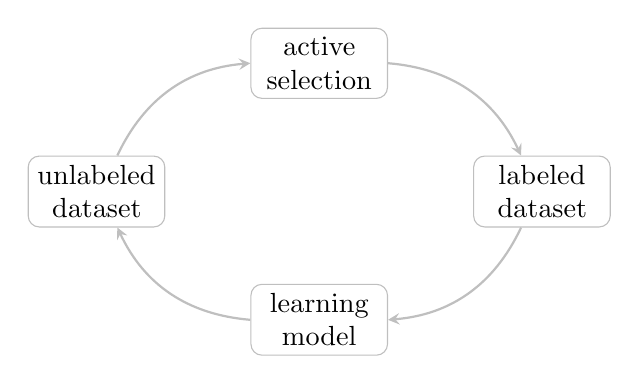
\begin{tikzpicture} [node distance = 4cm, on grid, auto]
 
\node (q0) [draw,lightgray, rounded corners, text width=1.5cm,yshift=-1.2cm, align =center] {\textcolor{black}{unlabeled \\dataset}};
\node (q1) [draw,lightgray, text width=1.5cm, rounded corners,above right = of q0,  yshift=-1.2cm,align =center] {\textcolor{black}{active \\selection}};
\node (q2) [draw,lightgray,rounded corners, text width=1.5cm, below right = of q1,yshift=1.2cm,align =center] {\textcolor{black}{labeled \\dataset}};
\node (q3) [draw,lightgray,rounded corners, text width=1.5cm, below left = of q2,yshift=1.2cm,align =center] {\textcolor{black}{learning \\model}};
 
\path [-stealth, thick]
    (q0) edge [lightgray, bend left]  (q1)
    (q1) edge [lightgray,bend left]  (q2)
    (q3) edge [lightgray,bend left]  (q0)
    (q2) edge [lightgray,bend left]  (q3);
\end{tikzpicture}
\caption{Active learning core structure. At each iteration a novel point is actively selected from the unlabeled set of data and the corresponding label is requested. Based on the received information, the model is modified.} \label{al}
\end{figure}

Indeed AL represents a training approach particularly suitable when labeled samples are too expensive or difficult to obtain. Specifically, AL is a particular ML algorithm based on a key idea: despite the shortage of labeled data, high accuracy results may be obtained if the training algorithm is allowed to choose the points to be labeled and learn from them \cite{settles1995active}. An AL algorithm asks an oracle to label the data considered most informative with an iterative approach. Doing so, since the queried points are directly selected by the learning algorithm, the amount of necessary labeled data is much smaller than that required for classical supervised ML approach. Figure \ref{al} shows the core structure of any AL algorithm: at each iteration the model is updated using the labelled dataset, and is allowed to ask for a new label in the unlabelled dataset. This process repeats until the model reaches sufficient performances or when the number of iterations reaches the maximum budget.

%\\In recent years, some active learning-based anomaly detection algorithms have been proposed.
%The idea of incorporating expert feedback in unsupervised anomaly detection algorithms aims at improving the achieved performance adding a relatively small computational cost. Active anomaly detection (AAD) algorithm \cite{das2016incorporating, das2017incorporating} proposes an active learning anomaly detection approach where points are ranked based on their anomalous behavior. The main goal is to maximize the number of true anomalies presented to the domain expert. An inclusion of AAD algorithm in the One Class Support Vector Machine (OCSVM) framework is tackled in \cite{lesouple2021incorporating}.
%Always using OCSVM, an expert feedback inclusion has been recently proposed %\cite{lesouple2021introduce}: to solve the problem, the paper combines together the $\mu$-SVM for the %labeled data and the OCSVM for the unlabeled set of data.

This paper focuses on the Isolation Forest detector, and suggests a strategy to tune it towards the user definition of anomaly. In this work the authors compare two AL query policies to ask the user new labels, and other two policies to update the internal structure with minimal computational effort. The goal is to increase the performance of the detector as much as possible, keeping very low both the labelling effort and the updating procedure. Moreover this method has two key advantages over the supervised and computationally expensive models: as it relies on an initial unsupervised training, it can start to work when there are no labels, but more importantly it can work even if instances from only one class are labelled. This is particularly useful when obtaining labels from the anomalous class is very uncommon or expensive.

%\gas{The rest of the papers is organized as follows: ...}
The rest of the paper is organized as follows. Initially, in Section \ref{rw} we outline the Isolation Forest in detail, and we indicate an existing active learning-based anomaly detection algorithm that will be used as a benchmark in thos work. Then, in Section \ref{pm} we illustrate the proposed model \approach: namely, we describe the strategies suggested to query the points as well as the approaches employed to update the model. In Section \ref{exp} we test \approach, comparing it with other models in relation to multiple real set of data. Finally, in Section \ref{conclusions} we draw conclusions for the present work.

%This paper compares two AL query strategies for anomaly detection using Isolation Forest. The algorithm key idea is to modify the internal structure of the unsupervised model based on a small amount of labeled data queried to the domain expert, trying to minimize the labelling effort but at the same time maximising the detection performance. Specifically, the presented model is based on the Isolation Forest model, i.e., the basic concept used to classify anomalies remains isolating data points from the rest of the dataset. Anyway, an innovative approach is used to query the labels and to update the model: novel information is achieved with the use of an active learning strategy by which the inner framework of the model is modified in order to match with the information obtained. Once the information is achieved, a user friendly iterative process allows to adapt the model by adjusting its structure on the basis of the novel input.
%The proposed method relies onto two distinguished yet essential issues: a process to select the most significant points and a tuning procedure to modify the structure of the model based on the information achieved. 
%This method has two key advantages over the supervised computationally expensive models: it is extremely computationally efficient and works even if instances from only one class are labelled.
%Based on the treated framework and on the data in hand, active learning algorithms are characterized by many possible query strategies \cite{settles1995active}. In this way, based on the considered purpose, the suitable query strategy may be selected and the corresponding most informative point may be labeled. 
%In the same way, we propose two possible approaches to address the selection of points to be labeled, producing two different query strategies with respect to both their benefits as well as their computational costs.
%\tommi{bisognerebbe scrivere che testiamo il nostro metodo su dataset reali e pubblichiamo il codice bla bla bla.}
%The importance of the algorithm...
%As we will see later the proposed model is based on...
%Section \ref{} ecc..
%list of the notation - simboli usati fare tabella





%\tommi{monitoring unexpected behaviour?} is essential. 
 %Even if, to date, there is no clear or official definition, broadly speaking, an anomalous point, also known as anomaly or outlier, is defined \textit{as an observation that deviates so much from other observations as to arouse suspicion that it was generated by a different mechanism} \cite{hawkins1980identification}. In general, an anomaly is identified as a variation from the norm, a data being characterised by a different behaviour with respect to other data that distinguishes itself from the rest of the dataset. Consequently, anomaly detection algorithms aim at detecting or identifying data that seem not to conduct themselves with a standard trend.
%\tommi{non sembra che parliamo di distribuzione gaussiana?}. 
%Anomaly detection techniques may be divided into three groups based on the available data in use: supervised, unsupervised and semi-supervised. 
%If the dataset contains labeled data, any technique for binary classification may be used, leading to highly accurate results. 
%Unfortunately, a critical challenge of anomaly detection is the lack of labeled data \cite{chandola2009anomaly}. Obtaining labels requires an often too expensive cost to take care of, since the labeling procedure is usually carried on by a human expert domain who, by hand labels each point with a time consuming and demanding routine. To solve this matter, semi-supervised or unsupervised techniques are employed. In the first scenario, a labeled portion of the original dataset is required, usually belonging to the most representative normal class, and, based on such labeled data, a model representing the normal behaviour is produced. \tommi{dici?} Generally, in fact, labeling normal data requires less efforts: normal points tend to have a common and more static behavior, making it easier to  be identified.
%For the classical unsupervised anomaly detection problem, the purpose is to isolate outliers with no use of labeled data based on the fact that normal data greatly outnumbers anomalous data. As a rule, unsupervised anomaly detection models are not tuned for the precise domain of application but are generally based on identifying rules based on specific data characteristics. 
%Based on the context and on the problem in question, different popular anomaly detection techniques exist. 
%\tommi{tornarci} A large class of unsupervised anomaly detectors are those based on statistical methods. These techniques produce a statistical distribution based on the given set of data and classify points according to where data falls: points that are not consistent or that simply lie in the tails of the computed distribution are consider anomalies \cite{hochenbaum2017automatic, hill2010anomaly}. 
%Some anomaly detection methods are based on the traditional classification problem. Based on the classical Support Vector Machine framework several methods have been proposed: the one-class support vector machine \cite{scholkopf1999support} computes an hyperplane that separates the data points from the origin and at the same time maximizes its distance with respect to the origin; the support vector data description \cite{tax2004support} looks for the smallest hypersphere containing the considered dataset. Distance-based \cite{knorr1998algorithms} and density-based \cite{breunig2000lof} outlier detection methods try to solve the problem by finding a profile for normal data based on inner data characteristics: the first uses the average distance of points, since, by nature, outliers have a higher value with respect to normal points; the latter is based on density area, due to the fact that outliers tend to stay in low density areas compared to normal points, which usually assemble in the same area. 

% tommi: andrei a capo in modo da evidenziare IF che è il metodo che andremmo ad analizzare
%A very popular anomaly detection algorithm is the Isolation Forest algorithm \cite{liu2008isolation, liu2012isolation}, which presents a brand-new approach: instead of creating a profile for normal data, it explicitly tries to isolate anomalies. To do it, Isolation Forest relies on two anomaly inner characteristics: they are fewer in number and they have very different attributes compared to normal data. 

%To cope with the lack of labeled data, in recent years some active learning-based anomaly detection algorithms have been proposed.
%The idea of incorporating expert feedback in unsupervised anomaly detection algorithms aims at improving the achieved performance adding a relatively small computational cost. Active anomaly detection (AAD) algorithm \cite{das2016incorporating, das2017incorporating} propose an active learning anomaly detection approach where points are ranked based on their anomalous behavior. The main goal is to maximize the number of true anomalies presented to the domain expert. An inclusion of AAD algorithm in the One Class Support Vector Machine (OCSVM) framework is tackled in \cite{lesouple2021incorporating}.
%Always using OCSVM, an expert feedback inclusion has been recently proposed \cite{lesouple2021introduce}. To solve the problem, the paper combines together the $\mu$-SVM for the labeled data and the OCSVM for the unlabeled set of data. 
%\cite{vercruyssen2018semi}. 


%This paper presents a novel active learning strategy for anomaly detection using Isolation Forest. The algorithm key idea is to modify the internal structure of the unsupervised model based on a small amount of labeled data queried to the domain expert, trying to minimize the labelling effort but maximising the detection performance. Specifically, the presented model is based on the Isolation Forest model, i.e., the basic concept used to classify anomalies remains isolating data points from the rest of the dataset. Anyway, an innovative approach is used to query the labels and to update the model: novel information is achieved with the use of an active learning strategy by which the inner framework of the model is modified in order to match with the information obtained. Once the information is achieved, a user friendly iterative process allows to adapt the model by adjusting its structure on the basis of the novel input.
%Based on the treated framework and on the data in hand, active learning algorithms are characterized by many possible query strategies \cite{settles1995active}. In this way, based on the considered purpose, the suitable query strategy may be selected and the corresponding most informative point may be labeled. 
%In the same way, we propose two possible approaches to address the selection of points to be labeled, producing two different query strategies with respect to both their benefits as well as their computational costs.
%\tommi{bisognerebbe scrivere che testiamo il nostro metodo su dataset reali e pubblichiamo il codice bla bla bla.}
%The importance of the algorithm...
%As we will see later the proposed model is based on...
%Section \ref{} ecc..
%list of the notation - simboli usati fare tabella

%
% vars
%
\newcommand{\X}{\ensuremath{\mathbf{X}}}
\newcommand{\B}{\ensuremath{\mathbf{B}}}
\newcommand{\Y}{\ensuremath{\mathbf{Y}}}
\newcommand{\Z}{\ensuremath{\mathbf{Z}}}
\newcommand{\Q}{\ensuremath{\mathbf{Q}}}
\newcommand{\Cb}{\ensuremath{\mathbf{C}}}
\newcommand{\V}{\ensuremath{\mathbf{V}}}
\newcommand{\A}{\ensuremath{\mathbf{A}}}
\newcommand{\x}{\ensuremath{\boldsymbol{x}}}
\newcommand{\bo}{\ensuremath{\boldsymbol{b}}}
\newcommand{\y}{\ensuremath{\boldsymbol{y}}}
\newcommand{\z}{\ensuremath{\boldsymbol{z}}}
\newcommand{\e}{\ensuremath{\boldsymbol{e}}}
\newcommand{\PC}{\ensuremath{\mathcal{C}}}
\newcommand{\PCaug}{\ensuremath{\mathcal{A}}}
\newcommand{\LC}{\ensuremath{\mathcal{L}}}
\newcommand{\WMCC}{\ensuremath{\mathcal{C}}}
\newcommand{\PSDD}{\ensuremath{\mathcal{C}}}
\newcommand{\AOMDD}{\ensuremath{\mathcal{C}}}
\newcommand{\PDG}{\ensuremath{\mathcal{C}}}
\newcommand{\primep}{\ensuremath{\mathsf{P}}}
\newcommand{\sub}{\ensuremath{\mathsf{S}}}
\newcommand{\CNET}{\ensuremath{\mathcal{C}}}
\newcommand{\C}{\ensuremath{\mathcal{C}}}
\newcommand{\CLT}{\ensuremath{\mathcal{T}}}
\newcommand{\model}{\ensuremath{\mathsf{m}}}
\newcommand{\modelfam}{\ensuremath{\mathcal{M}}}
\newcommand{\val}{\ensuremath{\mathsf{val}}}
\newcommand{\supp}{\ensuremath{\mathsf{supp}}}
\newcommand{\structure}{\ensuremath{\mathcal{G}}}
\newcommand{\tree}{\ensuremath{\mathcal{T}}}
\newcommand{\graph}{\ensuremath{\mathcal{G}}}
\newcommand{\params}{\ensuremath{\boldsymbol{\theta}}}
\newcommand{\sumparams}{\ensuremath{\boldsymbol{\theta}_{\mathsf{S}}}}
% \newcommand{\sumparams}{\ensuremath{\boldsymbol{\omega}}}
\newcommand{\leafparams}{\ensuremath{\boldsymbol{\theta}_{\mathsf{L}}}}
%\newcommand{\leafparams}{\ensuremath{\boldsymbol{\lambda}}}
\newcommand{\scope}{\ensuremath{{\phi}}}
\newcommand{\mixture}{\ensuremath{\mathcal{M}}}
\newcommand{\vtree}{\ensuremath{\mathcal{V}}}
% \newcommand{\p}{\ensuremath{\mathsf{Pr}}}
\newcommand{\p}{{p}}
\newcommand{\q}{{q}}
\newcommand{\m}{{m}}
\newcommand{\ch}{\ensuremath{\mathsf{in}}}
\newcommand{\pa}{\ensuremath{\mathsf{pa}}}
\newcommand{\leftn}{\ensuremath{\mathsf{L}}}
\newcommand{\rightn}{\ensuremath{\mathsf{R}}}% \newcommand{\f}{\ensuremath{f}}
\newcommand{\f}{\ensuremath{\Delta}}
\newcommand{\vtreenode}{\ensuremath{\mathcal{v}}}
\newcommand{\Ent}{\ensuremath{\mathbb{H}}}
\newcommand{\Mom}{\ensuremath{\mathbb{M}}}
\newcommand{\Ex}{\ensuremath{\mathbb{E}}}
\newcommand{\interval}{\ensuremath{\mathcal{I}}}
\newcommand{\Le}{\ensuremath{\mathsf{L}}}
\newcommand{\Ri}{\ensuremath{\mathsf{R}}}

\newcommand{\poly}[1]{\texttt{poly}(#1)}

%
% misc, writing
%
\newcommand{\eg}{e.g.,\ }
\newcommand{\wrt}{w.r.t.\ }
\newcommand{\ie}{i.e.,\ }
\newcommand{\cf}{cf.\ }
\newcommand{\aka}{a.k.a.\ }
\newcommand{\iid}{i.i.d.\ }

%
% symbols, concepts
\newcommand{\prob}{\ensuremath{\mathsf{Pr}}}
\newcommand{\uprob}{\ensuremath{{\bwidetilde{\mathsf{P}}\mathsf{r}}}}

%
% operators
\newcommand{\vars}{\ensuremath{\mathsf{vars}}}
\newcommand{\id}[1]{\llbracket{#1}\rrbracket}
\newcommand{\neigh}{\ensuremath{\mathsf{neigh}}}

\newcommand{\mathL}{\mathcal{L}}
\newcommand{\mathP}{\mathcal{P}}
% \newcommand{\E}{\mathcal{E}}
\newcommand{\data}{\mathcal{D}}
\newcommand{\F}{\mathcal{F}}
\newcommand{\mi}{\text{MI}}
\newcommand{\true}[0]{\texttt{true}}
\newcommand{\false}[0]{\texttt{false}}
\newcommand{\oplusl}{\operatornamewithlimits{\oplus}}
\newcommand{\otimesl}{\operatornamewithlimits{\otimes}}
\newcommand{\landl}{\operatornamewithlimits{\land}}

%
\newcommand{\flow}{\mathrm{F}}
\newcommand{\expflow}{\mathrm{EF}}
\newcommand{\context}{\gamma}
\newcommand{\pseudocount}{\alpha}
\newcommand{\bigO}{\mathcal{O}}
\newcommand{\bigOmega}{\Omega}
\newcommand{\bigTheta}{\Theta}
\newcommand{\indicator}[1]{\mathbbm{1}[#1]}
\newcommand{\weight}[2]{\mathtt{weight}(#1,#2)}
\newcommand{\entropy}{\mathtt{ENT}}
\newcommand{\expectation}{\mathbb{E}}
\newcommand{\LL}{\mathtt{LL}}
\newcommand{\lit}{\mathtt{Lit}}

\newcommand{\pluseq}{\mathrel{+}=}
\newcommand{\minuseq}{\mathrel{-}=}

\newcommand{\w}{\mathbf{w}}
\newcommand{\W}{\mathbf{W}}

\newcommand{\bp}{\mathbf{p}}

\newcommand{\SL}{\mathrm{L}^{\mathrm{s}}}
\newcommand{\WSL}{\mathrm{L}^{\mathrm{ws}}}
\newcommand{\MC}{\mathtt{MC}}

%
% queries
\newcommand{\nlquery}[2]{\begin{minipage}{.07\textwidth}$q_{#1}:$\end{minipage}\begin{minipage}{.88\textwidth}\raggedright\emph{#2}\end{minipage}}

\newcommand{\SPLIT}{\mathtt{SPLIT}}

\newcommand{\given}{\vert}
%\SL{------ Working Sections -----}


\section{Revisiting Machine Unlearning and Evaluation}
\label{sec: primer_MU}



\iffalse 
In this section, we begin by formulating the problem of {\MU} (machine unlearning) and     reviewing  unlearning methods regarded as baselines in this work. Next, we  revisit how the
%provide a holistic understanding of 
unlearning performance can be assessed using diverse and    complementary  metrics.
\fi 


\noindent \textbf{Problem setup.}
MU aims to remove ({or} scrub) the influence of some targeted training data on a trained ML model \cite{cao2015towards,bourtoule2021machine}. 
\iffalse 
%trained over the entire training set. 
This problem was  raised for protecting data privacy 
%the     private data information contained in the training set 
\citep{cao2015towards,bourtoule2021machine}, in particular in coming forth with legislation like  General Data Protection Regulation (GDPR) \cite{hoofnagle2019european} and  California Consumer Privacy Act (CCPA) \cite{pardau2018california}. It can also be viewed as a method of understanding dataset influence
%\PR{dataset influence?}
in model training
%analysis method to understand the dataset 
\cite{koh2017understanding}. 
\fi 
%We elaborate on its mathematical formulation below. 
%of {\MU} below.
%of the MU problem is illustrated below.
Let $\mathcal{D} = \{\mathbf z_i \}_{i=1}^N$ be a (training) dataset of $N$  data points, with label information encoded for supervised learning. $\Df \subseteq \mathcal D$ represents  a subset whose influence we want to scrub, termed
%. We term  $\Df $ 
the \textbf{forgetting dataset}.
%typically with a  less number of data points than  $\mathcal D$, 
%\textit{e.g.}, the set of data points  in  a single class with sensitive data content to be scrubbed. 
Accordingly, the complement of $\Df$ is the \textbf{remaining dataset}, \textit{i.e.}, $\Dr = \mathcal D \setminus \mathcal{D}_{\mathrm{f}}$.
We denote by $\btheta$ the model parameters, and $\thetafull$   the \textbf{original  model} trained    on the entire training set  $\mathcal D$ using \textit{e.g.}, empirical risk minimization (ERM). Similarly, we denote by $\thetaunl$  an \textbf{unlearned model}, obtained by a scrubbing algorithm, after    removing the influence of $\Df$ from the  trained model $\thetafull$. The \textbf{problem of MU} is to find an accurate and efficient  scrubbing mechanism  to generate  $\thetaunl$   from  $\thetafull$. 
In existing studies \cite{golatkar2020eternal,graves2021amnesiac,bourtoule2021machine}, the choice of the forgetting dataset $\Df$ specifies different unlearning scenarios. 
There exist two main categories. 
{First}, \textit{class-wise forgetting} \cite{golatkar2020eternal,graves2021amnesiac} refers to  unlearning $\Df$ consisting of training data points of an entire class. 
% Second, \textit{random data forgetting (per class)} \cite{golatkar2020eternal} refers to unlearning $\Df$   given by a subset of data points randomly selected from a single class, \textit{e.g.}, the basic backdoor data poisoning setup in \SL{\cite{gu2017badnets,liu2022backdoor}}. 
Second, \textit{random data forgetting} corresponds to unlearning $\Df$  given by a  subset of random data drawn from all classes.
%\JH{delete random data forgetting (one class)}



% {\color{cyan}
% \noindent \textbf{Different unlearning scenarios.}
% There are various unlearning scenarios in the machine unlearning area. Here we summarize them into three main categories based on how the forgetting dataset is selected. 

% \ding{70} \textit{Class-wise forgetting} \cite{golatkar2020eternal,graves2021amnesiac}
% The forgetting dataset $D_f$ contains one class.


% \ding{70} \textit{Random data forgetting (per-class)} \cite{golatkar2020eternal}
% $D_f$ only contains a subset of data points from a single class. 



% \ding{70} \textit{Random data forgetting (all-class)} \cite{bourtoule2021machine}
% $D_f$ contains data points randomly selected from all classes.
%}
%given $\Df$ and $\mathcal D$. 
% \PS{redundant sentences}
%
% We express the above unlearning process  as
% $
%  \thetaunl  \overset{\mathrm{MU}}{\longleftarrow} S( \thetafull, \Df, \mathcal D )
% $.
% \begin{align}
%     \thetaunl  \overset{\mathrm{MU}}{\longleftarrow} S( \thetafull, \Df, \mathcal D ).
% \end{align}
%

\noindent \textbf{Exact and approximate MU methods.} The \textit{exact unlearning}  method refers to 
%the ground-truth scrubbing strategy of 
\textit{retraining} the model parameters  from \textit{scratch} over the remaining dataset $\Dr$. 
%We call this exact method   \textbf{\retrain} and denote the resulting unlearned model by $\thetaEU$.
Although retraining from scratch (that we term  \textbf{\retrain})
is optimal for MU, it entails a large computational overhead, particularly for DNN training. This problem is alleviated by \textit{approximate unlearning}, an easy-to-compute proxy for {\retrain}, which has received growing attention.
%For ease of presentation, the model parameters of using approximate unlearning is denoted by  
Yet,   the boosted computation efficiency   comes at the cost of  MU's  efficacy. %Thus, the development of effective   approximate unlearning methods is now a major research focus. 
We next review some commonly-used approximate unlearning methods that we improve in the sequel by leveraging sparsity; see a summary in  \textbf{Tab.\,\ref{tab: summary_MU_methods_metrics}}. 

%\PS{$\thetafull$ is fixed but $\thetaunl$ is method dependent. So, should we differentiate different $\thetaunl$'s in the following description, e.g., $\thetaunl^{\text{FT}}$, $\thetaunl^{\text{GA}}$, $\thetaunl^{\text{FF}}$, etc. to avoid confusion.}


%will serve as our baselines.\PR{``... methods we will improve in the sequel by leveraging sparsity.''}

%$\bhq$

\begin{wraptable}{r}{70mm}
\vspace*{-4.5mm}
        \centering
         \caption{\footnotesize{Summary of approximate unlearning methods considered in this work. 
         %We also listed five evaluation metrics to evaluate machine unlearning performance. 
         The marker `\textcolor{black}{\ding{51}}' denotes the metric used in previous research. The number in {\RTE} is the   run-time cost reduction compared to the  cost of {\retrain}, based on our empirical studies in Sec.\,\ref{sec: exp} on %with the data-model setup 
         (CIFAR-10, ResNet-18). Note that 
         {\GA} seems better than ours in terms of RTE, but it is less effective in unlearning.
         %\PS{Maybe we can add one sentence clarifying (for the eager-to-judge reviewer) that even though GA seems better in terms of RTE, but the performance loss compared to ours offsets its gain.}
         %in Sec.\,\ref{sec: exp}. 
         %\SL{[change back to Representative work]}
        % \SL{[no need to specify venue, replacing it with Representative work. add more refs? and add `our work'? \SL{Concern on complexities?}]}
         } 
         }
\vspace*{-2mm}
        \label{tab: summary_MU_methods_metrics}
        \resizebox{0.50\textwidth}{!}{
        \begin{tabular}{c|ccccc|c}
        \toprule
        Unlearning &  \multicolumn{5}{c|}{Evaluation metrics} & \multirow{2}{*}{Representative work}\\
        Methods &  \UA& \MIAF & \RA & \TA & \RTE & \\
        \midrule
        FT & \textcolor{black}{\ding{51}} & & \textcolor{black}{\ding{51}}& \textcolor{black}{\ding{51}}& 0.06$\times$ & \cite{golatkar2020eternal,warnecke2021machine}    \\
        GA &  \textcolor{black}{\ding{51}}& \textcolor{black}{\ding{51}}& \textcolor{black}{\ding{51}}& \textcolor{black}{\ding{51}}& 0.02$\times$ &  \cite{graves2021amnesiac,thudi2021unrolling}  \\
        FF & \textcolor{black}{\ding{51}} & & \textcolor{black}{\ding{51}}& \textcolor{black}{\ding{51}}& 0.9
        %\SL{?}
        $\times$ & \cite{golatkar2020eternal,becker2022evaluating}    \\
        \IU & \textcolor{black}{\ding{51}} & & &\textcolor{black}{\ding{51}} & 0.08$\times$ &  \cite{koh2017understanding,izzo2021approximate} \\
        \midrule
        Ours & \textcolor{black}{\ding{51}} & \textcolor{black}{\ding{51}}&\textcolor{black}{\ding{51}} & \textcolor{black}{\ding{51}}& 0.07$\times$ & This work  \\
        \bottomrule
        \end{tabular}}
\vspace*{-7.5mm}
\end{wraptable}
\noindent\ding{70} \textit{Fine-tuning (\textbf{\FT})} \cite{golatkar2020eternal,warnecke2021machine}:  
Different from    {\retrain}, {\FT} fine-tunes the   pre-trained  model   $\thetafull$ on {$\Dr$} using a few training epochs to obtain ${\thetaunl}$. The rationale is that fine-tuning on {$\Dr$} initiates the catastrophic forgetting in  the model over {$\Df$} as is common in continual learning \cite{parisi2019continual}. 

\noindent\ding{70} \textit{Gradient ascent (\textbf{\GA})} \cite{graves2021amnesiac,thudi2021unrolling}:
{\GA} reverses the model training on  %the forgetting dataset 
$\Df$ by adding the corresponding gradients    back to  $\thetafull$, \textit{i.e.}, moving $\thetafull$  in the direction of increasing  loss for   data points to be scrubbed. 
%The unlearning error of using GA was also approximated and bounded  by \citet{thudi2021unrolling} in the scenario of unlearning a single data point.  

%  is the opposite of gradient de- scent performed to train the model normally.
% we fine-tune on D by moving in the direction of increasing loss for samples in Df , which is equivalent to using a negative gradient for the samples to forget. This aims to damage features predicting Df correctly. 


\noindent \ding{70} \textit{Fisher forgetting (\textbf{\FF})}  \cite{golatkar2020eternal,becker2022evaluating}:
{\FF} adopts  an  additive Gaussian noise  to `perturb'   $\thetafull$ towards   exact unlearning.
%model from {\retrain}.
%\PS{But how do we know the model from \retrain?} 
Here the Gaussian distribution has zero mean  and covariance determined by  the $4$th root of Fisher Information matrix with respect to (w.r.t.) $\thetafull$ on   $\Dr$.
%We note that the computation of the Fisher Information matrix could lower the  efficiency of {\FF} on GPUs
We note that the computation of the Fisher Information matrix exhibits lower parallel efficiency in contrast to other unlearning methods, resulting in higher computational time when executed on GPUs; see
\citet{golatkar2020eternal} for implementation details. %\SL{Why is slow?}


\noindent \ding{70} \textit{Influence unlearning (\textbf{\IU})} \cite{koh2017understanding,izzo2021approximate}:
{\IU} leverages the influence function approach \cite{cook1982residuals} to characterize the change in  $\thetafull$  if a training point is removed from the training loss. {\IU} estimates the change in model parameters from $\thetafull$ to $\thetaunl$, \textit{i.e.}, $\thetaunl - \thetafull$.  {{\IU} also relates to an important line of research in MU, known as $\epsilon$-$\delta$ forgetting \cite{wang2022federated,guo2019certified,xu2023machine}. However, it typically requires additional model and training assumptions \cite{guo2019certified}. 
%the application of $\epsilon$-$\delta$ forgetting is limited to linear finetuning of Deep Learning (DL) models \cite{guo2019certified}. Furthermore, it necessitates alterations to the model training pipeline \cite{guo2019certified}. Such constraints are not congruent with our objective of efficiently approximating unlearning on pre-trained DL models. Given these inherent limitations and misalignment with our goals, we have chosen not to compare methods from the $\epsilon$-$\delta$ forgetting domain in our paper. 
}
%as derived in Proposition\,\ref{prop: IU}.

We next take a step further to revisit the {\IU} method and re-derive its formula (\textbf{Prop.\,\ref{prop: IU}}), with the aim of enhancing the effectiveness of existing  solutions proposed in the previous research.

\iffalse
Specifically, let us consider a \textit{weighted} ERM training, yielding   the optimization problem $\btheta(\mathbf w) = \argmin_{\btheta} L(\mathbf w, \btheta)$, where $L(\mathbf w, \btheta) = \sum_{i=1}^N [w_i \ell_i (\btheta, \mathbf z_i)]$. 
%\PS{We can change $\ell_i$ to $\ell$, since the dependence on $i$ is already present in $\mathbf z_i$} 
Here
%we explicitly express the learned model as a function of the data influence weights $\mathbf w$,  
$\ell_i (\btheta, \mathbf z_i)$ is the training loss of $\btheta$  on the data point $\mathbf z_i$,   $w_i \in [0,1]$ is the influence weight associated with $\mathbf z_i$, and $\mathbf 1^T \mathbf w = 1$.
%$L(\mathbf w, \btheta) = \sum_{i=1}^N [w_i \ell_i (\btheta, \mathbf z_i)]$, where $\btheta$ is the variable of model parameters,  $\ell_i (\btheta, \mathbf z_i)$ is the training loss of $\btheta$  on the data point $\mathbf z_i$,   $w_i \in [0,1]$ is the influence weight associated with $\mathbf z_i$ during training, and $\mathbf 1^T \mathbf w = 1$.
Based on the above, the non-scrubbed (original) model  is   given by $\thetafull = \btheta(\mathbf 1/N)$,  and the exactly unlearned model by {\retrain} is  $\thetaunl = \btheta(\mathbf{1}_{\Dr}/\mathrm{card}(\Dr))$, 
% $\thetaunl = \argmin_{\btheta} L(\mathbf{1}_{\Dr}/\mathrm{card}(\Dr), \btheta)$, 
where $\mathbf{1}_{\Dr}\in\mathbb \{ 0,1\}^N$  is the binary vector whose $i$th element is $1$ if the $i$th data point belongs to $\Dr$ and $0$ otherwise, and $\mathrm{card}(\Dr)$ is the cardinality of $\Dr$.   {\IU} then  estimates the change in model parameters from $\thetafull$ to $\thetaunl$, \textit{i.e.}, $\thetaunl - \thetafull$, as derived in Proposition\,\ref{prop: IU}.
%\PS{Do we want to keep this result here, given that this section is more of an overview, and this is our proof?}

% $L(\mathbf w, \btheta) = \sum_{i=1}^N [w_i \ell_i (\btheta, \mathbf z_i)]$, where $\btheta$ is the variable of model parameters,  $\ell_i (\btheta, \mathbf z_i)$ is the training loss of $\btheta$  on the data point $\mathbf z_i$,   $w_i \in [0,1]$ is the influence weight associated with $\mathbf z_i$ during training, and $\mathbf 1^T \mathbf w = 1$. Based on the above, the model trained on the full dataset is   given by $\thetafull = \argmin_{\btheta} L( \mathbf 1/N, \btheta)$, and {\retrain} yields 
% $\thetaunl = \argmin_{\btheta} L(\mathbf{1}_{\Dr}/\mathrm{card}(\Dr), \btheta)$, where $\mathbf{1}_{\Dr}\in\mathbb \{ 0,1\}^N$  is the (element-wise) binary vector whose $i$th element is $1$ if the $i$th data point belongs to $\Dr$ and $0$ otherwise, and $\mathrm{card}(\Dr)$ denotes the cardinality of $\Dr$. The {\IU} method aims to estimate the change in model parameters from $\thetafull$ to $\thetaunl$, \textit{i.e.}, $\Delta = \thetaunl - \thetafull$. We show the estimator of $\Delta$ of using {\IU} in Proposition\,\ref{prop: IU}.
\fi


\begin{myprop}
\label{prop: IU}
Given the weighted ERM training $\btheta(\mathbf w) = \argmin_{\btheta}
L(\mathbf w,\btheta)
%\sum_{i=1}^N [w_i \ell_i (\btheta, \mathbf z_i)]
$ where $L(\mathbf w,\btheta) = \sum_{i=1}^N [w_i \ell_i (\btheta, \mathbf z_i)]$, 
$w_i \in [0,1]$ is the influence weight associated with the data point $\mathbf z_i$ and $\mathbf 1^T \mathbf w = 1$, 
%\revision{let $L(\mathbf w,\btheta) = \sum_{i=1}^N [w_i \ell_i (\btheta, \mathbf z_i)]$} for convenience,  
the  model update from   $\thetafull$  to $\btheta(\mathbf w)$ yields %\YL{anyway we can explain briefly the "approximation" power? it seems weird to use the approximation without explaining in a proposition..}
% \vspace*{-5mm}
{\small\begin{align}
   \hspace*{-2mm} \Delta(\mathbf w) \Def   \btheta(\mathbf w) - \thetafull \approx  \mathbf H^{-1} {\color{black}{  \nabla_{\btheta} L( \mathbf 1/N - \mathbf w, \thetafull)  }},  
  \hspace*{-2mm}
  \label{eq: Delta_IU}
\end{align}}%
where $\mathbf 1$ is the $N$-dimensional vector of all ones, {$\mathbf w=\mathbf{1}/N$ signifies the uniform weights used by ERM}, $\mathbf H^{-1} $ is the inverse of the Hessian    $\nabla^2_{\btheta,\btheta} L(\mathbf 1/N,  \thetafull)$ evaluated at $ \thetafull$, and $\nabla_{\btheta} L$ is the gradient of $L$. When scrubbing $\Df$, the unlearned model is given by
$\thetaunl = \thetafull + \Delta(\mathbf{w}_\mathrm{MU})$. Here  
%$\mathbf w_{\mathrm{MU}} = \mathbf{1}_{\Dr}/\mathrm{card}(\Dr)$,
$\mathbf w_{\mathrm{MU}} \in [0, 1]^{N}$ with entries $w_{\mathrm{MU},i} = \mathbb{I}_{\Dr } (i) / |\Dr|$ signifying the data influence weights for {\MU}, %$\Dr = \mathcal D \setminus \mathcal{D}_{\mathrm{f}}$, 
$\mathbb{I}_{\Dr } (i) $ is the indicator function with value 1 if $i \in \Dr $ and 0 otherwise, and $|\Dr|$ is the cardinality of $\Dr$.
\end{myprop}
% {\scriptsize \textcolor{red}{PS: $\mathbf w$ should be $N$-dimensional, so I guess $\mathbf w_{\mathrm{MU}}$ should be $N$-dimensional with $w_{\mathrm{MU}} (i) = 0$ if $i \in \mathcal{D}_{\mathrm{f}}$ and $w_{\mathrm{MU}} (i) = 1/|\mathcal{D}_{\mathrm{r}}|$ else. Also, if you're using ``card'' for cardinality, mention this explicitly.}}
%
%\vspace*{-0.5mm}
\textbf{Proof}: We derive \eqref{eq: Delta_IU}  using an implicit gradient approach;
%Different from  existing proofs in \cite{koh2017understanding,izzo2021approximate,warnecke2021machine}, we derive \eqref{eq: Delta_IU} from a bi-level optimization viewpoint; 
see Appendix\,\ref{appendix: IU}.
% \SL{[@Jinghan, @Jiancheng; add proof details using our current notations in Appendix.]}
\hfill $\square$
%\vspace*{-1.8mm}
%\end{myprop}


%\SL{[Missing remark on computing of  inverse Hessian-gradient product. ]}

It is worth noting that we have taken into consideration the weight normalization effect $\mathbf 1^T \mathbf w =1$ 
 in  \eqref{eq: Delta_IU}. This is   different from  existing work like \citet[Sec.\,3]{izzo2021approximate} using Boolean or unbounded weights. In practice, we found that {\IU} with  weight normalization can improve the unlearning performance. 
Furthermore, 
to update the model influence given by \eqref{eq: Delta_IU}, one needs to acquire the second-order information in the form of  inverse-Hessian gradient product. Yet, the exact computation is prohibitively expensive. To overcome this issue, we use the first-order WoodFisher approximation \cite{singh2020woodfisher} to estimate  the inverse-Hessian gradient product. 
%of high accuracy.

\noindent \textbf{Towards a `full-stack' {\MU} evaluation.}
Existing work   has assessed  {\MU} performance from different aspects \cite{thudi2021unrolling,golatkar2020eternal,graves2021amnesiac}. 
%\revision{In particular, Golatkar\citep{golatkar2020eternal} proposed `read-out' function to assess the performance of machine unlearning.} 
%,  such as the Euclidean distance between an unlearned model $\thetaunl$  and the exactly unlearned model \cite{thudi2021unrolling},  the accuracy of   $\thetaunl$ on  $\Df$ \cite{golatkar2020eternal}, and membership inference of $\thetaunl$ on  $\Df$ \cite{graves2021amnesiac}. 
Yet, a single  performance metric may provide   a limited %\PS{``limited'', ``incomplete''?}
view of {\MU} \cite{thudi2022necessity}. 
\iffalse 
For example, it was shown in \cite{thudi2022necessity} that the unlearning error in the parameter space (given by the Euclidean distance between an unlearned model and retrained one) could give us a false sense of successful unlearning since it might be possible to   unlearn without modifying the model at all \YL{i think the above sentence is confusing: is it true that you can unlearn without modifying the model? that sounds unlikely..or did you mean that minimizing the unlearning error defined above can return an unmodified model }. 
\fi 
%which leads to a large Euclidean  distance from the exactly unlearned model.
%Thus,  precisely evaluating the performance of {\MU}   remains a challenge. 
By carefully reviewing the prior art, we focus on the following empirical metrics (summarized in  Tab.\,\ref{tab: summary_MU_methods_metrics}).

\noindent \ding{70} \textit{Unlearning accuracy (\textbf{\UA})}: 
% Given by the  accuracy  of an unlearned model $\thetaunl$  on the forgetting dataset $\Df$ (denoted by $\mathrm{Acc}_{\Df} (\thetaunl)$), 
We define $\mathrm{\UA}(\thetaunl) = 1-\mathrm{Acc}_{\Df} (\thetaunl)$ to characterize the \textit{efficacy} of {\MU} in the accuracy dimension, where $\mathrm{Acc}_{\Df} (\thetaunl)$ is the  accuracy  of $\thetaunl$ on the forgetting dataset  $\Df$ \cite{golatkar2020eternal,graves2021amnesiac}.
It is important to note that a more favorable {\UA}   for an approximate unlearning method should   \textbf{reduce its performance disparity  with  the gold-standard retrained model (\retrain)}; a higher value is not necessarily better. This principle also extends to other evaluation metrics.

%Note that a better {\UA}  for   an approximate unlearning method signifies a smaller gap with {\UA} of  the gold-standard retrained model ({\retrain}). This also applies to other metrics.


% Since $\thetaunl$ is expected  to scrub  the influence of $\Df$ in $\thetafull$, we expect $\mathrm{Acc}_{\Df}(\thetaunl) < \mathrm{Acc}_{\Df}(\thetafull) \Rightarrow \mathrm{\UA}(\thetaunl) > \mathrm{\UA}(\thetafull)$.   
%$\mathrm{Acc}_{\Df} (\thetaunl)$ should be \textit{lower} than the accuracy of the unlearned model $\thetafull$ on $\Df$, yielding $\mathrm{\UA}(\thetaunl) > \mathrm{\UA}(\thetafull)$.

\noindent \ding{70} \textit{Membership inference attack (MIA)  on  $\Df$ (\textbf{\MIAF})}:   This is another metric   to assess the \textit{efficacy} of unlearning.
It is achieved by applying the   confidence-based MIA predictor \cite{song2019privacy,yeom2018privacy} to the unlearned model ($\thetaunl$) on the forgetting dataset ($\Df$). The MIA success rate can then indicate how many samples in $\Df$ can be correctly predicted as forgetting (\textit{i.e.}, non-training) samples of $\thetaunl$.
 A \textit{higher} {\MIAF}   implies    less information about   $\Df$     in $\thetaunl$; see Appendix\,\ref{appendix: metric settings} for more details.





% achieved by   MIA %(against $\thetaunl$) 
% to determine whether or not a data point in $\Df$ belongs to the training set of  $\thetaunl$ \cite{wu2022puma,chen2021machine}. A \textit{higher} {\MIAF}   implies that  less information about   $\Df$ contained in $\thetaunl$.
% \JC{For detailed formulations of {\MIAF}, please refer to Appendix\,\ref{appendix: metric settings}.}


%\SL{[refer to appendix for detailed formulations.]}

%\PS{All other metrics are accuracy or efficiency. However, it's not clear from the name \textbf{\MIAF} what it is. Can we call it ``MIA efficacy''?}


\iffalse 
It is also worth noting that one can similarly define {\MIAR}, given by   the MIA rate on the remaining dataset $\Dr$.  However, different from {\MIAF}, {\MIAR}  characterizes the   \textit{privacy}   of $\thetaunl$ about $\Dr$. A \textit{lower} {\MIAR} rate implies less information leakage from   $\thetaunl$ on $\Dr$.
\fi 

%$\mathrm{\UA}(\thetaunl)$ should be  higher than $\mathrm{Acc}_{\Df} (\thetafull)$

%The scrubbed model should contain as little information as possible about the target data


\noindent \ding{70} \textit{Remaining accuracy (\textbf{\RA})}:   This refers to 
the accuracy of {$\thetaunl$} on $\Dr$, which reflects the \textit{fidelity} of    {\MU} 
 \cite{becker2022evaluating}, {\textit{i.e.}, training data information}  should be  preserved from {$\thetafull$} to {$\thetaunl$}. 

%It is desired to preserve this accuracy after {\MU} 
%the fidelity of    {\MU} on  $\Dr$, \textit{i.e.}, 
%is preserved after {\MU}.
%\cite{becker2022evaluating}.

\noindent \ding{70} \textit{Testing accuracy (\textbf{\TA})}:  This measures the \textit{generalization} ability of {$\thetaunl$} on  a testing dataset rather than $\Df$ and $\Dr$. {{\TA} is evaluated on the whole test dataset, except for class-wise forgetting, in which testing data points belonging to the forgetting class are not in the testing scope. 
%By contrast, testing accuracy (TA) is evaluated on testing points from all non-forgetting classes in the class-wise forgetting scenario. 
}


%\ding{176} \textit{Membership inference attack rate on  $\Dr$ (\textbf{MIA}-$\Dr$)}:   


\noindent \ding{70} \textit{Run-time efficiency (\textbf{\RTE})}:  This measures the computation efficiency of an {\MU} method.  For example,
if we regard the run-time cost of  {\retrain} as the baseline, the computation acceleration gained by different approximate unlearning methods is summarized in Tab.\,\ref{tab: summary_MU_methods_metrics}.

%Note that the  run-time cost of  {\retrain}  provides the upper bound of the computation complexity in the algorithm design of {\MU}.



%Table\,\ref{tab: summary_MU_methods_metrics} summarizes the {\MU} methods and metrics that we reviewed. 
\iffalse 
Since the best unlearning efficacy  is achieved by {\retrain}, our aim in the next section is to reduce the gap between  approximate unlearning and {\retrain}. 
%while maintaining the former's run-time efficiency.
\fi 
% \SL{[@Jinghan @Jiancheng, please add a well-organized table here. You can get some inspiration \href{https://openreview.net/pdf?id=MjsDeTcDEy}{Table 1}.]}


% \begin{table}[t]
%         \centering
%          \caption{\footnotesize{Summary of 4 existing machine unlearning methods considered in this work. We also listed five evaluation metrics to evaluate machine unlearning performance. The Symbol `\textcolor{black}{\ding{51}}' denotes the metric used in the representative works. The number in {\RTE} demonstrates the relative time cost compared to retrain method.  \SL{[no need to specify venue, replacing it with Representative work. add more refs? and add `our work'? \SL{Concern on complexities?}]}}  }
%         \label{tab: summary_MU_methods_metrics}
%         \resizebox{0.45\textwidth}{!}{
%         \begin{tabular}{c|ccccc|c}
%         \toprule
%         Unlearning &  \multicolumn{5}{c|}{Evluation metrics} & \multirow{2}{*}{Representative work}\\
%         Methods &  \UA& \MIAF & \RA & \TA & \RTE & \\
%         \midrule
%         FT & \textcolor{black}{\ding{51}} & & \textcolor{black}{\ding{51}}& \textcolor{black}{\ding{51}}& 1.00& \cite{golatkar2020eternal,warnecke2021machine}  \\
%         GA &  \textcolor{black}{\ding{51}}& \textcolor{black}{\ding{51}}& \textcolor{black}{\ding{51}}& \textcolor{black}{\ding{51}}& 0.07 &  \cite{graves2021amnesiac,thudi2021unrolling} \\
%         FF & \textcolor{black}{\ding{51}} & & \textcolor{black}{\ding{51}}& \textcolor{black}{\ding{51}}& 0.92& \cite{golatkar2020eternal,becker2022evaluating}   \\
%         \IU &  & & & & 0.08 & \cite{koh2017understanding,izzo2021approximate}\\
%         \midrule
%         Ours & \textcolor{black}{\ding{51}} & \textcolor{black}{\ding{51}}&\textcolor{black}{\ding{51}} & \textcolor{black}{\ding{51}}& 0.07 & This Work \\
%         \bottomrule
%         \end{tabular}}
% \end{table}


% \begin{table}[htb]
%         \centering
%          \caption{\footnotesize{Summary of approximate unlearning methods considered in this work. 
%          %We also listed five evaluation metrics to evaluate machine unlearning performance. 
%          The marker `\textcolor{black}{\ding{51}}' denotes the metric used in the corresponding references. The number in {\RTE} demonstrates the   run-time improvement compared to {\retrain}.  
%         % \SL{[no need to specify venue, replacing it with Representative work. add more refs? and add `our work'? \SL{Concern on complexities?}]}
%          } 
%          }
%         \label{tab: summary_MU_methods_metrics}
%         \resizebox{0.45\textwidth}{!}{
%         \begin{tabular}{c|ccccc|c}
%         \toprule
%         Unlearning &  \multicolumn{5}{c|}{Evluation metrics} & \multirow{2}{*}{Difficulty for parameter tuning}\\
%         Methods &  \UA& \MIAF & \RA & \TA & \RTE & \\
%         \midrule
%         FT & \textcolor{black}{\ding{51}} & & \textcolor{black}{\ding{51}}& \textcolor{black}{\ding{51}}& 0.07$\times$ & Easy to tune the learning rate (1)   \\
%         GA &  \textcolor{black}{\ding{51}}& \textcolor{black}{\ding{51}}& \textcolor{black}{\ding{51}}& \textcolor{black}{\ding{51}}& 0.02$\times$ &  Sensitive to the learning rate (3) \\
%         FF & \textcolor{black}{\ding{51}} & & \textcolor{black}{\ding{51}}& \textcolor{black}{\ding{51}}& 0.92$\times$ & Sensitive to fisher information coefficient. (4)   \\
%         \IU &  & & & & 0.08$\times$ & Sensitive to parameters for hessian approximation (2) \\
%         \midrule
%         Ours & \textcolor{black}{\ding{51}} & \textcolor{black}{\ding{51}}&\textcolor{black}{\ding{51}} & \textcolor{black}{\ding{51}}& 0.07$\times$ & Unlearning Methods Agnostic  \\
%         \bottomrule
%         \end{tabular}}
% \end{table}





\section{
% Why Model Sparsity for {\MU}?
Model Sparsity: A Missing Factor Influencing Machine Unlearning
}
\label{sec: sparsityMU}

%\SL{[I stop here.]}

%This section shows that model sparsity is a missing factor influencing {\MU}.

%explore the effect of model sparsity (achieved by weight pruning) on {\MU}, demonstrating how  pruning can improve   unlearning in   theory and practice.




\noindent \textbf{Model sparsification via weight pruning.}
% Weight pruning promotes model  sparsity by
% %aims to reduce model sizes by 
% removing  redundant model parameters.
% %\textit{i.e.}, promoting model  sparsity.
% As shown in many prior studies \cite{han2015deep, blalock2020state,chen2021lottery,frankle2018lottery,frankle2020linear,ma2021sanity,zhang2022advancing},  
Model sparsification could not only facilitate  a model's training, inference, and deployment  but also benefit model's performance. For example, LTH (lottery ticket hypothesis) \cite{frankle2018lottery} stated that a trainable sparse sub-model  could be identified from the original dense model, with test accuracy on par or even better than the original model. 
%\PS{This para has lot of overlap with the first para of page 2, including description of LTH. Can be shortened.}
% There also exist many ways to find the desired sparse models,  ranging from pruning at random initialization before training \cite{tanaka2020pruning,frankle2020pruning} to pre-trained weights-based magnitude pruning \cite{ma2021sanity,frankle2018lottery}.
\textbf{Fig.\,\ref{fig: OMP_results}} shows an example of  the pruned model's generalization   vs. its   sparsity ratio. Here  one-shot magnitude pruning (\textbf{OMP}) \cite{ma2021sanity} is adopted to obtain sparse models. 
OMP is computationally the lightest pruning method, which   directly prunes the model weights to the target sparsity ratio based on their magnitudes. As we can see, there exists a graceful sparse regime  with lossless testing accuracy.
%the generalization performance of three commonly-used weight pruning methods 

\iffalse 
\begin{table}[h]
\caption{\footnotesize{OMP trajectory given by test accuracy (\%) VS. sparsity (\%) of ResNet-18 on CIFAR-10 dataset. \SL{Still needs improvement.}}}
\resizebox{0.45\textwidth}{!}{
\begin{tabular}{c|c|c|c|c|c|c|c}
\toprule
   Sparsity  & 0 & 50 & 75 & 90 &95&99&99.5  \\
   \midrule
     \TA& 94.57 & 94.83&94.73&94.76&94.24&92.28&90.05 \\
     \bottomrule
\end{tabular}}
\label{tab: OMP_results}
\end{table}
\fi 
% \begin{figure}[htb]


\begin{wrapfigure}{r}{45mm}
\vspace*{-5mm}
%\vspace*{-6mm}
\centerline{
\includegraphics[width=45mm,height=!]{figs/OMP_on_CIFAR-10_ResNet18.pdf}
}
\vspace*{-2mm}
\caption{\footnotesize{
{Testing accuracy  of   OMP-based sparse ResNet-18   vs. the   dense model on CIFAR-10. 
%The  line  represents the mean  of test accuracies over 5 independent trials.
}
}}
  \label{fig: OMP_results}
 \vspace*{-5mm}
\end{wrapfigure}
\noindent \textbf{Gains of {\MU} from sparsity.}
We first analyze the impact of model sparsity on {\MU}  through a lens of   \textit{unrolling stochastic gradient descent} (\textbf{SGD}) \cite{thudi2021unrolling}. The specified SGD method allows us to derive the \textit{unlearning error} (given by the  weight difference between the approximately unlearned model   and the
gold-standard retrained model)  when scrubbing a single data point. However, different from \citet{thudi2021unrolling}, we  will infuse the model sparsity into  SGD unrolling. 


Let us assume a binary mask $\mathbf m$ associated with the model parameters $\btheta$, where $m_i = 0$ signifies that the $i$th parameter 
 $\theta_i$ is pruned to zero and $m_i = 1$  represents the unmasked   $\theta_i$.  This sparse pattern $\mathbf m$ could be obtained by a weight pruning method, like OMP. 
 %in Fig.\,\ref{fig: OMP_results} 
 %\PS{why refer to fig 2 here?}. 
Given $\mathbf m$,   the \textbf{sparse model}  is $ \mathbf m \odot \btheta $, where $\odot$ denotes the element-wise multiplication. Thudi \emph{et al.}\,\cite{thudi2021unrolling} showed that if 
%$\btheta^\prime = \btheta$ (\textit{i.e.}, $\mathbf{m} = \mathbf 1$) and  
{\GA} is adopted to scrub a single data point for the original (dense) model $ \btheta$ (\textit{i.e.}, $\mathbf{m} = \mathbf 1$),  then  the gap between {\GA} and {\retrain} can be approximately bounded in the weight space. 
  \textbf{Prop.\,\ref{prop: SGD_sparse_MU}} extends the existing unlearning error analysis   to a    sparse model. 

%error $e$ (\textit{i.e.}, the  weight difference from  {\retrain}) can be  bounded by

\iffalse 
\vspace*{-5mm}
{\small \begin{align}
   \hspace*{-2mm} e(\btheta_0, \{ \hat{\mathbf z}_i \},  t, \eta) 
 %\nonumber \\
=  \eta^2 \sum_{i=1}^{t-1} [ \nabla_{\btheta,\btheta}^2\ell(\btheta_0, \hat{\mathbf z}_i ) \sum_{j=0}^{i-1}   \nabla_{\btheta} \ell(\btheta_0, \hat{\mathbf z}_j ) ],
 \hspace*{-3mm}
 \label{eq: err_MU_SGD}
\end{align}}%
where $\btheta_0$ is  model initialization when using SGD-based ERM training,    $\{ \hat{\mathbf z}_i \}$
is the sequence of stochastic data samples, $t$ is the number of training iterations, $\eta$ is the learning rate, $\nabla_{\btheta,\btheta}^2\ell(\btheta_0, \hat{\mathbf z}_j)$ is the stochastic Hessian of the training loss $\ell$ evaluated at $\btheta_0$ and the  sample $\hat{\mathbf z}_j$.
Built upon \eqref{eq: err_MU_SGD}, 
%In the following 
Prop.\,\ref{prop: SGD_sparse_MU}  shows the    unlearning error   of {\GA} on a sparse model.
\fi 

%\SL{[Updated prop. Please check.]}
\begin{myprop}
\label{prop: SGD_sparse_MU}
Given the model sparse pattern $\mathbf m$ and the SGD-based  training, the unlearning error   of  {\GA}, denoted by $e(\mathbf m)$, can be characterized by the weight distance
between the {\GA}-unlearned model and the gold-standard retrained model. This leads to the error bound
\iffalse 
and 
 \underline{$ e_{\Omega_{\mathbf m}}(\btheta_0, \{ \hat{\mathbf z}_i \},  t, \eta) $}, where
 $e_{\Omega_{\mathbf m}}$ 
signifies the subvector of $e$ in \eqref{eq: err_MU_SGD} with coordinates given by the unmasked index set $\Omega_m$,  and $\Omega_{\mathbf{m}} = \{ i: m_i = 1 \}$ is the index set of unmasked parameters.
\fi 
%
% \vspace*{-5mm}
% {\small\begin{align}
%   \|  e^\prime(\btheta_0^\prime, \{ \hat{\mathbf z}_i \},  t, \eta)  \|_2 =
%   \|  e_{\Omega_{\mathbf m}}(\btheta_0, \{ \hat{\mathbf z}_i \},  t, \eta) \|_2 ,
%   \label{eq: MU_err_m}
% \end{align}}
% where $\btheta_0^\prime = \mathbf m \odot \btheta_0$,
% $\Omega_{\mathbf{m}} = \{ i: m_i = 1 \}$ is the index set of unmasked parameters, {\color{cyan}and  $e_{\Omega_{\mathbf m}}$ refers to the subvector of $e$ in \eqref{eq: err_MU_SGD} with coordinates given by the unmasked index set $\Omega_m$.}
%
%And the Euclidean norm of the unlearning error can be approximately bounded by
%modifies \eqref{eq: err_MU_SGD} to 
%\begin{align}
\iffalse
  $  e^\prime(\btheta_0^\prime, \{ \hat{\mathbf z}_i \},  t, \eta) \Def \mathbf m \odot e(\btheta_0, \{ \hat{\mathbf z}_i \},  t, \eta) $, where $e$ is  defined in  \eqref{eq: err_MU_SGD}.  
  \fi 
%\end{align}
%$\mathbf m \odot e(\btheta_0, \{ \hat{\mathbf z}_i \},  t, \eta) $. 
%an approximate     upper bound of the above  error is  given by
% \begin{align}
%     e(\mathbf m, \btheta_0, \{ \hat{\mathbf z}_i \},  t, \eta) 
% \end{align}

\vspace*{-5mm}
{\small\begin{align}
  % \|   e_{\Omega_{\mathbf m}}(\btheta_0, \{ \hat{\mathbf z}_i \},  t, \eta)  \|_2 
  e(\mathbf m) = \mathcal{O}(\eta^2 t  \| 
   \mathbf m \odot (\btheta_t - \btheta_0) \|_2 \sigma(\mathbf m) )
  % \leq \frac{\eta}{2}{(t-1) \|    \mathbf m \odot (\btheta_t - \btheta_0) \|_2}  \sigma(\mathbf m),
   \label{eq: err_bd_SGD_sparse}
\end{align}}%
where $\mathcal O$ is the big-O notation, $\eta$ is the learning rate, 
$t$ is the number of   training iterations, 
$ (\btheta_t - \btheta_0)$ denotes the weight difference at iteration $t$ from its   initialization $\btheta_0$,  and
$\sigma(\mathbf m)  $ is the largest singular value ($\sigma$) of the  Hessian $\nabla_{\btheta,\btheta}^2\ell$ (for a training loss $\ell$)   among the  unmasked parameter dimensions, \textit{i.e.}, $\sigma(\mathbf m) \Def \max_{j} \{  \sigma_{j}( \nabla_{\btheta,\btheta}^2\ell ), \text{if } m_j \neq 0  \}$.
%Here   $\sigma_j (\mathbf A)$ is the $j$th singular value of a matrix $\mathbf A$.

\textbf{Proof}: 
See Appendix\,\ref{appendix: SGD_sparse_MU}. 
%\SL{[ @Pranay, @Jinghan, @Jiancheng. Please check and use the above notations to complete the proof in appendix]}
\hfill $\square$
\end{myprop}
% \begin{myprop}
% \label{prop: SGD_sparse_MU}
% Given the model sparse pattern $\mathbf m$ and the SGD-based  training over the non-zero model weights in $\btheta^\prime$, the unlearning error of   {\GA} to scrub a single data point yields
% %modifies \eqref{eq: err_MU_SGD} to 
% %\begin{align}
%   $  e^\prime(\btheta_0^\prime, \{ \hat{\mathbf z}_i \},  t, \eta) \Def \mathbf m \odot e(\btheta_0, \{ \hat{\mathbf z}_i \},  t, \eta) $, where $e$ is  defined in  \eqref{eq: err_MU_SGD}.  
% %\end{align}
% %$\mathbf m \odot e(\btheta_0, \{ \hat{\mathbf z}_i \},  t, \eta) $. 
% An approximate     upper bound of the above  error is  given by
% % \begin{align}
% %     e(\mathbf m, \btheta_0, \{ \hat{\mathbf z}_i \},  t, \eta) 
% % \end{align}
% \begin{align}
%    \|   e^\prime(\btheta_0^\prime, \{ \hat{\mathbf z}_i \},  t, \eta)  \|_2 \leq \frac{\eta (t-1) \| \btheta_t - \btheta_0 \|_2}{2}  \sigma(\mathbf m),
%    \label{eq: err_bd_SGD_sparse}
% \end{align}
% where $\sigma(\mathbf m)  $ is the largest singular value of the stochastic Hessian $\nabla_{\btheta,\btheta}^2\ell$ given in \eqref{eq: err_MU_SGD} among the  model dimensions unpruned, \textit{i.e.}, $\sigma(\mathbf m) \Def \max_{j} \{  \sigma_{j}( \nabla_{\btheta,\btheta}^2\ell ), \text{if } m_j \neq 0  \}$. Here   $\sigma_j (\mathbf A)$ denotes the $j$th singular value of the matrix $\mathbf A$.
% \end{myprop}
We next draw some key insights   from \textbf{Prop.\,\ref{prop: SGD_sparse_MU}}. \textit{First},  it is clear from  \eqref{eq: err_bd_SGD_sparse} that the unlearning error reduces as the model sparsity in $\mathbf m$ increases. 
By contrast, the unlearning error  derived in  \citet{thudi2021unrolling} for a  dense model  (\textit{i.e.}, $\mathbf{m} = \mathbf 1$) is proportional to the dense model distance $\| \btheta_t - \btheta_0 \|_2$. 
%yields $O(\eta^2 t \| \mathbf{w}_t - \mathbf w_0 \|_2 \sigma(\mathbf 1))$.
%Recall that this unlearning error is given by the distance from the exact unlearned model.   
Thus,   model sparsity  is beneficial to reducing the gap between ({\GA}-based) approximate and exact unlearning. 
\textit{Second}, the error bound \eqref{eq: err_bd_SGD_sparse}  enables us to relate {\MU} to the  spectrum of the  Hessian  of the loss landscape. 
%Proposition\,\ref{prop: SGD_sparse_MU} that  the error term $\sigma(\mathbf m)$ in \eqref{eq: err_bd_SGD_sparse} characterizes the influence of model sparsity in {\MU}.  First, 
The number of active singular values (corresponding to nonzero dimensions in $\mathbf m$) decreases when the sparsity grows.
However, it is important to note that in a high-sparsity regime, the model's generalization   could   decrease. Consequently, it is crucial to  select the model sparsity to strike a balance between generalization   and unlearning performance.

% \SL{[Needs to clarify not  the sparser the better due to generalization loss.]}
% On the other hand, the magnitudes of these singular values also decrease since weight pruning can reduce the sharpness of the loss landscape; see  supporting  results in \textbf{Fig.\,\ref{fig: singular_sparsity}}.
%\SL{[Let us decide at the end if we should   move this to appendix.]}
%\PS{Is there a way to show this theoretically, since currently, in (4) we only observe decrease in number of active singular values.} 
% Such pruning effect has also been  justified by existing studies, \textit{e.g.},     %the reduced sharpness of the Hessian   \cite{chen2022can} and 
% the linear model connectivity of sparse models   \cite{frankle2020linear}. 
%The aforementioned insights from   \eqref{eq: err_bd_SGD_sparse}  also justify    that the unlearning error decreases as the sparsity of $\mathbf m$ increases; \PS{Isn't the last sentence redundant with first few sentences in this para?}


%Therefore, our key insight  from Proposition\,\ref{prop: SGD_sparse_MU} is that     model sparsity can contribute to reducing the gap between {\GA}-based approximate unlearning and exact unlearning. 

%the   error of  the {\GA}-based approximate unlearning method. 

%if the model is not pruned (\textit{i.e.}, $\mathbf m = \mathbf 1$), then 

%We provide some  insights   drawn from Proposition\,\ref{prop: SGD_sparse_MU} on the influence of model sparsity in {\MU}.  

% \begin{figure}[htb]
% %\begin{wrapfigure}{r}{80mm}
% %\vspace*{-6mm}
% \centerline{
% %\begin{tabular}{cc}
% %\hspace*{0mm}\includegraphics[width=.3\textwidth,height=!]{figure/performance_comparison.pdf}  
% %&
% %\hspace*{-4mm}
% \includegraphics[width=.31\textwidth,height=!]{example-image-a}
% % \\
% % \hspace*{2mm}\footnotesize{(a) Test accuracy vs. pruning ratio.} &   \footnotesize{(b) Runtime of pruning.}
% %\end{tabular}
% }
% \vspace*{-3mm}
% \caption{\footnotesize{
% TBD. 
% }}
%   \label{fig: singular_sparsity}
% %  \vspace*{-3.8mm}
% %\end{wrapfigure}
% %\end{figure}
% \end{figure}


\begin{figure*}[t]
% \vspace*{-3mm}
\centerline{
\begin{tabular}{cccc}
    \hspace*{-2mm}  \includegraphics[width=0.25\textwidth,height=!]{figs/ua.pdf} &
    \hspace*{-5mm} \includegraphics[width=0.25\textwidth,height=!]{figs/mia.pdf} &
    \hspace*{-5mm} \includegraphics[width=0.25\textwidth,height=!]{figs/ra.pdf} &
    \hspace*{-5mm}  \includegraphics[width=0.25\textwidth,height=!]{figs/ta.pdf} 
\end{tabular}}
 \vspace*{-3mm}
\caption{\footnotesize{
%\SL{[Figure needs updating.]} %\JC{"Retain" -> "Remain"}
Performance of approximate unlearning ({\FTC}, {\GAC}, {\FFC}, {\IUC}) and exact unlearning ({\retrainC}) in efficacy ({\UA} and {\MIAF}), fidelity ({\RA}), and generalization ({\TA}) vs. model sparsity (achieved by {OMP}) in the data-model setup (CIFAR-10, ResNet-18). 
The unlearning scenario is class-wise 
 forgetting, and 
the average unlearning  performance over 10 classes is reported. We remark that being closer to \textcolor{red}{Retrain} performance is better for approximate MU schemes.
% \JC{TODO: Remove legend in fig 3c}
%\PS{See comment in the last para of Section 3. Are we trying to forget an entire class?}
}}
\vspace*{-7mm}
\label{fig: results_OMP_MU}
\end{figure*}

Inspired by Prop.\,\ref{prop: SGD_sparse_MU}, we ask: 
\textit{Does the above   benefit of model sparsification in {\MU} apply to   other approximate unlearning methods besides {\GA}?} This drives us to investigate the performance of approximate unlearning across the entire spectrum as depicted in  {Tab.\,\ref{tab: summary_MU_methods_metrics}}.
%unlearning on sparse models through our   multi-criteria evaluation in \textbf{Tab.\,\ref{tab: summary_MU_methods_metrics}}.
% conduct  the  all-dimension unlearning performance assessment 
% on sparse models, where evaluation metrics have been listed   in Table\,\ref{tab: summary_MU_methods_metrics}. 
Therefore,
\textbf{Fig.\,\ref{fig: results_OMP_MU}} shows the unlearning efficacy ({\UA} and {\MIAF}), fidelity ({\RA}), and generalization ({\TA}) of different   approximate unlearning methods   in the sparse model regime. Here class-wise forgetting is considered for {\MU} and OMP is used for weight pruning. 
% to 
% remove the influence of   all data points in one class from models pruned to different sparsity levels using OMP.
%\PS{We're trying to forget all the points from one class, right? This is not clear from this sentence.}
% on  OMP-based %\PS{``based''?}
% sparse models at different sparsity ratios. \PS{How about: ``... to remove the influence of all the data points belonging to a particular class from models pruned to different sparsity levels using OMP.''?}
%The performance of exact unlearning via {\retrain} is   provided for comparison. 
As we can see, the efficacy of approximate unlearning is significantly improved as the model sparsity increases, \textit{e.g.},   {\UA} and {\MIAF} of using {\FT} over 90\% sparsity.  By contrast, {\FT} over the dense  model (0\% sparsity) is the least effective for {\MU}. 
%\PS{Why do we mention FT alone? The same conclusion seems to hold for GA, FF, IU as well.}
%We also note that the efficacy  of {\retrain} is resilient to model sparsity. 
Also, the efficacy gap between exact unlearning ({\retrain}) and  approximate unlearning  reduces on sparse models. Further, through the fidelity and generalization lenses, {\FT} and {\FF} yield the {\RA} and {\TA}  performance closest to {\retrain}, compared to other unlearning methods. In the regime of ultra-high  sparsity (99\%), 
the efficacy of unlearning exhibits a tradeoff with  {\RA} and {\TA} to some extent.   
%For example, at the $95\%$-sparsity  regime, 

% presents our evaluation results  on {OMP}-based sparse models used in Fig.\,\ref{fig: OMP_results}. 
% % empirically study   the performance metrics  of   {\MU} methods  (Table\,\ref{tab: summary_MU_methods_metrics}) when applied to     sparse models given by OMP   in  Fig.\,\ref{fig: OMP_results}. Fig.\,\ref{fig: results_OMP_MU} shows our full-dimension assessments of {\MU} against model sparsity. 
% As we can see, \SL{[list key principled results.]}


% \begin{figure}[htb]
% \vspace*{-3mm}
% \centerline{
% \begin{tabular}{cccc}
%     \hspace*{-5mm}  \includegraphics[width=.23\textwidth,height=!]{figs/ua.pdf} &
%     \hspace*{-5mm} \includegraphics[width=.23\textwidth,height=!]{figs/mia.pdf} \\
    
%     \hspace*{-5mm} \includegraphics[width=.23\textwidth,height=!]{figs/ra.pdf} &
%     \hspace*{-5mm}  \includegraphics[width=.23\textwidth,height=!]{figs/ta.pdf} 
% \end{tabular}}
%  \vspace*{-3mm}
% \caption{\footnotesize{
% %\SL{[Figure needs updating.]} %\JC{"Retain" -> "Remain"}
% Performance of approximate unlearning ({\FTC}, {\GAC}, {\FFC}, {\IUC}) and exact unlearning ({\retrainC}) in efficacy ({\UA} and {\MIAF}), fidelity ({\RA}), and generalization ({\TA}) vs. model sparsity (achieved by {OMP}) in the data-model setup (CIFAR-10, ResNet-18). 
% The unlearning scenario is class-wise 
%  forgetting, and 
% the average unlearning  performance over 10 classes is reported. 
% %\PS{See comment in the last para of Section 3. Are we trying to forget an entire class?}
% }}
% % \vspace*{-3mm}
% \label{fig: results_OMP_MU}
% \end{figure}



\section{Sparsity-Aided Machine Unlearning}
\label{sec: sparsity_MU_alg}



%In the previous section, we showed that model sparsification could be a principled approach of reducing the gap between approximate unlearning and exact unlearning. 
Our study in Sec.\,\ref{sec: sparsityMU} suggests the new  {\MU} paradigm `prune first, then unlearn', which leverages the fact that  (approximate) unlearning on a sparse model yields a smaller unlearning error (Prop.\,\ref{prop: SGD_sparse_MU}) and improves the efficacy of {\MU}   (Fig.\,\ref{fig: results_OMP_MU}).
This promising finding, however, raises some new questions.  First, it remains elusive how the choice of a weight pruning method impacts the unlearning performance. Second,
%besides unlearning on a     sparse model,
it leaves room for developing  {sparsity-aware} {\MU} methods that can directly scrub data influence from a dense model.  %This section will address these two questions.
 



\noindent \textbf{Prune first, then unlearn: Choice of pruning methods.}
  % Our study in Sec.\,\ref{sec: sparsityMU} suggested the new  {\MU} paradigm `prune first, then unlearn', which shed light on that  (approximate) unlearning on a sparse model   yields a smaller unlearning error (Prop.\,\ref{prop: SGD_sparse_MU}) and improves the efficacy  of {\MU}   (Fig.\,\ref{fig: results_OMP_MU}).
  % Yet, 
  There exist many ways to find the desired sparse model
in addition to OMP. Examples include pruning at random
initialization before training \cite{tanaka2020pruning,frankle2020pruning}
 and simultaneous pruning-training iterative magnitude pruning (\textbf{IMP}) \cite{frankle2018lottery}.
  %Yet, there   exist many ways 
  %iterative magnitude pruning (\textbf{IMP}) \cite{ma2021sanity,frankle2018lottery}. 
  Thus, the problem of pruning method selection arises for {\MU}. From the viewpoint of {\MU},  the unlearner would prioritize a pruning method that satisfies the following criteria:  \ding{182} \textit{least dependence}  on the forgetting dataset ($\Df$), \ding{183} \textit{lossless generalization} when pruning, and \ding{184} \textit{pruning efficiency}. The rationale behind \ding{182} is  that  
  %since {\MU} targets scrubbing the influence of $\Df$ in the trained model, 
  it is desirable \textit{not} to incorporate    information of $\Df$ when seeking a sparse model prior to unlearning. 
  %\PS{This point is not clear to me. Additional info such as?} 
  And the criteria \ding{183} and \ding{184} ensure that sparsity cannot hamper {\TA} (testing accuracy)  and {\RTE} (run-time efficiency). 
  %which are also desired for {\MU} in addition to efficacy and fidelity (see Table\,\ref{tab: summary_MU_methods_metrics}).
  Based on \ding{182}-\ding{184}, 
  we   propose to use two pruning methods.  
  %in the `prune first, then unlearn' paradigm. 

\noindent  \ding{70} \textbf{SynFlow} (synaptic flow pruning) \cite{tanaka2020pruning}: 
SynFlow provides a (training-free) pruning method at initialization, even without   accessing the dataset. %to identify highly sparse sub-models  at initialization. 
Thus, it is uniquely suited for {\MU} to meet  the criterion \ding{182}. And SynFlow is easy to compute and yields a generalization improvement over many other pruning-at-initialization methods; see justifications in \cite{tanaka2020pruning}.


  
\noindent \ding{70} \textbf{OMP} (one-shot magnitude pruning)  \cite{ma2021sanity}: 
Different from SynFlow, {OMP}, which we focused on in Sec.\,\ref{sec: sparsityMU},
is performed over the original model   ($\thetafull$). It may depend on
%relate to \PS{``depend on''?}
%and thus  relates to 
the forgetting dataset ($\Df$), but has a much weaker dependence compared to {IMP}-based methods.
%Yet, such a relationship is much looser than     {IMP}-based methods \cite{frankle2018lottery}.
%that we have introduced and used in Sec.\,\ref{sec: sparsityMU} 
Moreover, {OMP} is  computationally lightest (\textit{i.e.}  best for \ding{184}) and    can yield better generalization than {SynFlow} \cite{zhang2022advancing}.
%Fig.\,\ref{fig: OMP_results} and Fig.\ref{fig: results_OMP_MU}


\begin{wrapfigure}{r}{72mm}
\vspace*{-4.5mm}
\centerline{
\begin{tabular}{cccc}
\hspace*{-5mm} \includegraphics[width=35mm,height=!]{figs/UA_vs_pruning_retrain.pdf} &
    \hspace*{-5mm}  \includegraphics[width=35mm,height=!]{figs/MIA_vs_pruning.pdf} 
    \hspace*{-3mm} 
\end{tabular}}
 \vspace*{-3mm}
\caption{\footnotesize{Influence of different   pruning
methods ({\color{red}{SynFlow}}, {\color{ForestGreen}{OMP}}, and {\color{blue}{IMP}}) in unlearning efficacy ({\UA} and {\MIAF}) and generalization ({\TA})  on    (CIFAR-10, ResNet-18). \textbf{Left}: {\UA} vs. {\TA}. \textbf{Right}:   {\MIAF} vs. {\TA}. Each point is a {\FT}-based unlearned dense or sparse model (75\% or 95\% sparsity), or a retrained dense model.
%using  {\FT}. \JC{If a pruning method is proper for {\MU}, then its integration with {\FT} should  yield unlearned models with closer {\UA}, {\MIAF}, and {\TA} to {\retrain}.} 
%\JC{larger font in figs}
}}
 \vspace*{-4mm}
\label{fig: results_pruning_comparison}
\end{wrapfigure}
Furthermore, it is important to clarify that IMP (iterative magnitude pruning) is \textit{not} suitable for {\MU}, despite being widely used to find the most accurate sparse models (\textit{i.e.}, best for criterion \ding{183}).
% Next, we would like to highlight that IMP is not proper for {\MU} although it is the predominant approach to find the most accurate sparse models (\textit{i.e.},     best for \ding{183}). 
 % We also remark that in the research on model pruning, IMP   is   the predominant approach to find the most accurate sparse models (\textit{i.e.},     best for \ding{183}). 
 Compared with the proposed pruning methods, IMP has the largest computation overhead   and the strongest correlation with the training dataset (including $\Df$), thereby deviating from \ding{182} and \ding{184}.
 %due to its pruning-retraining iterations. 
 % In this sense, IMP may not be a proper  pruning choice for {\MU} through the lenses of \ding{182} and \ding{184}. 
 In \textbf{Fig.\,\ref{fig: results_pruning_comparison}}, we show  the   efficacy  of {\FT}-based unlearning on sparse models generated  using  different pruning methods (SynFlow, OMP, and IMP). 
 %where {\FF} is used as the unlearning algorithm.
 %the unlearning setup remains the same as Fig.\,\ref{fig: results_OMP_MU}.  
 As we can see, unlearning on {SynFlow} or {OMP}-generated sparse models yields improved {\UA} and {\MIAF} over that on the original dense model and   {IMP}-generated sparse models.  This unlearning improvement over the dense model is consistent with Fig.\,\ref{fig: results_OMP_MU}. More interestingly, we find that {IMP} \textit{cannot} benefit the unlearning efficacy, although it leads to the best {\TA}. This is because {IMP} heavily relies on the training set including forgetting data points, which is revealed by the empirical results -- the unlearning metrics get worse for IMP with increasing sparsity.
 %\textit{i.e.}, violating the criterion \ding{182}. 
 %We will  show a fix to {IMP} for {\MU} later.
 Furthermore, when examining the performance of SynFlow and OMP, we observe that the latter   generally outperforms the former, exhibiting results that are closer to those of {\retrain}. 
 %in {\TA} with  similar unlearning efficacy.  
 Thus,  \textit{{OMP} is the pruning method we will use by default}. 
 
 
 %at the model sparsity ratios 75\% and 95\%
 
 %compared to SynFlow and IMP, 
 
 %\SL{[add experiment analysis and distilled unlearning principles/insights. @Jiancheng, @Jinghan]}



%% While IMP is powerful, it requires multiple cycles of
%expensive training and pruning with very specific sets of hyperparameters.


%%% empirical results



%To this end, we  propose two sparsity-aware (approximate) unlearning methods below.

%built upon sparsity-regularized optimization   and pruning-unlearning alternative optimization (AO), respectively.  

%
\begin{wrapfigure}{r}{35mm}
\vspace*{-3mm}
\includegraphics[width=35mm,height=!]{figs/magnitude.pdf}
\caption{\JC{Magnitude trend of the model weights during unlearning.}
\SL{Move to an appendix or delete.}}
\label{fig: l1_weight_magnitude}
\vspace*{-3mm}
\end{wrapfigure}
{\noindent \textbf{Sparsity-aware  unlearning.}}
% \JH{Add discussion about schedulers of $\gamma$, refer to table\,\ref{tab: ablation_l1_scheduler}.Also add some figures to show changes of magnitude.}
%In the   `prune first, then unlearn' paradigm, model sparsity is given \textit{a priori} for {\MU}. 
We next study if pruning and unlearning can be carried out simultaneously, without requiring prior knowledge of model sparsity. Let $\Lunl (\btheta; \thetafull,  \Dr)$ denote the unlearning objective function of model parameters $\btheta$, given the pre-trained  state $\thetafull$, 
%the overall training dataset $\mathcal D$, 
and the remaining training dataset $\Dr$. %Recall that $\Lunl $ can be specified by any {\MU} method studied in Sec.\,\ref{sec: primer_MU}. 
Inspired by  sparsity-inducing optimization \cite{bach2012optimization}, we integrate an $\ell_1$ norm-based sparse penalty into  $\Lunl $. This leads to the problem of `\textbf{\MUSparse}':

\vspace*{-3mm}
{\small{\begin{align}
    \thetaunl = \argmin_{\btheta} \Lunl (\btheta; \thetafull,  \Dr) + \gamma \| \btheta \|_1,
    \label{eq: MUSparse}
\end{align}}}%
where we specify $\Lunl$ by the fine-tuning objective, and $\gamma > 0$ is a regularization parameter that {controls the penalty level of the $\ell_1$ norm, thereby reducing the magnitudes of `unimportant' weights.}

%\noindent \textbf{\JC{Ablation study on parameter scheduler in \MUSparse.}}
% However, as \citep{bach2012optimization} mentioned, the downside of $\ell_1$ regulation term will affect the is its loss  in {\RA} and {\TA} compared to {\FT} and {\retrain}. Therefore, we conducted a comprehensive study of the scheduler of $\lambda$ in {\MUSparse}. In \textbf{Tab.\,\ref{tab: ablation_l1_scheduler}}, we present the results of unlearning performance on different parameter schedulers: constant scheduler, linear growing scheduler, and linear decaying scheduler.
% It shows that the decaying $\gamma$ scheduler performs the best among all the schedulers. If we directly apply a constant $\lambda$ to {\MUSparse}, it will either get a low {\UA} with lower $\lambda$ (for $\lambda = 0$, the method reduces to {\FT}) or worse {\RA} and {\TA} 
%  under higher $\lambda$. In Tab.\,\ref{tab: ablation_l1_scheduler}, we picked a sweet point to get a balance between them. If we use the linear growing scheduler, which means the method focuses on the unlearning term first then moves the focus to sparsity. If we use the linear decaying scheduler, the method focuses on the unlearning term first then moves the focus to sparsity.
\iffalse
\begin{wraptable}{R}{80mm}
\centering
\vspace*{-4.25mm}
\caption{\footnotesize{{\MU} performance  comparison of using {\MUSparse} with different   sparsity schedulers of $\gamma$  in \eqref{eq: MUSparse} and using {\retrain}.  
The unlearning scenario is given by random data forgetting (10\% data points across all classes) on (ResNet-18, CIFAR-10).
%considering various unlearning scenarios on CIFAR10 dataset. The content format follows Tab.\,\ref{tab: overall_perfoamnce}.
%Bold numbers indicate the closest performance to {\retrain}, and
A performance gap  against \textcolor{blue}{{\retrain}} is provided 
%. The relative drop or improvement represented 
in (\textcolor{blue}{$\bullet$}).
}}
\label{tab: ablation_l1_scheduler}
% \vspace*{0.1in} % Requirements, do not delete.
\resizebox{0.57\textwidth}{!}{
\begin{tabular}{c|c|c|c|c|c}
\toprule[1pt]
\midrule
  {\MU}& {\UA} & {{\MIAF}}& {{\RA}} & {{\TA}} & {{RTE} (min)} \\ 

% \cline{3-10}

% \midrule
% \rowcolor{Gray}
% \multicolumn{6}{c}{Class-wise forgetting} \\
% \midrule
% {\retrain} & \textcolor{blue}{100.00} & \textcolor{blue}{100.00} & \textcolor{blue}{100.00} & \textcolor{blue}{94.83} & 43.23
% \\
% {\MUSparse} + constant $\gamma$ & 100.00 (\textcolor{blue}{0.00}) & 100.00 (\textcolor{blue}{0.00}) & 91.69 (\textcolor{blue}{8.31})	& 87.3 (\textcolor{blue}{7.53}) & 2.61
% \\
% {\MUSparse} +   growing $\gamma$  & 100.00 (\textcolor{blue}{0.00}) & 100.00 (\textcolor{blue}{0.00}) & 94.43 (\textcolor{blue}{5.57})	& 88.43 (\textcolor{blue}{6.40}) & 2.61
% \\
% {\MUSparse} +   decaying $\gamma$ & 100.00 (\textcolor{blue}{0.00}) & 100.00 (\textcolor{blue}{0.00}) & \textbf{98.99} (\textcolor{blue}{\textbf{1.01}})	& \textbf{93.40} (\textcolor{blue}{\textbf{1.43}}) & 2.61
% \\
% \midrule
% \rowcolor{Gray}
% \multicolumn{6}{c}{Random data forgetting (all classes)} \\
\midrule
{\retrain} & \textcolor{blue}{5.41} & \textcolor{blue}{13.12} & \textcolor{blue}{100.00} & \textcolor{blue}{94.42} & 42.15
\\
%  \FT & $6.83$ (\textcolor{blue}{$1.42$}) & $14.97$ (\textcolor{blue}{$1.85$})& $96.61$ (\textcolor{blue}{$3.39$})& $90.13$ (\textcolor{blue}{$4.29$})  & 2.33 
% \\		
% \IU & $2.03$ (\textcolor{blue}{$3.38$})&  $5.07$ (\textcolor{blue}{$8.05$})& $98.26$ (\textcolor{blue}{$1.74$})& $\textbf{91.33}$ (\textcolor{blue}{$\textbf{3.09}$}) & 3.22
% \\
{\MUSparse} + constant $\gamma$ & 6.60 (\textcolor{blue}{1.19}) & 14.64 (\textcolor{blue}{1.52}) & 96.51 (\textcolor{blue}{3.49})	& 87.30 (\textcolor{blue}{7.53}) & 2.53
\\

{\MUSparse} + linear growing $\gamma$  & 3.80 (\textcolor{blue}{1.61}) & 8.75 (\textcolor{blue}{4.37}) & 97.13 (\textcolor{blue}{2.87})	& 90.63 (\textcolor{blue}{3.79}) & 2.53
\\
{\MUSparse} + linear decaying $\gamma$ & \textbf{5.35} (\textcolor{blue}{\textbf{0.06}}) & \textbf{12.71} (\textcolor{blue}{\textbf{0.41}}) & \textbf{97.39} (\textcolor{blue}{\textbf{2.61}})	& {\textbf{91.26}} (\textcolor{blue}{\textbf{3.16}}) & 2.53
\\
\midrule
\bottomrule[1pt]
\end{tabular}
}
\vspace*{-4mm}
\end{wraptable}
\fi
\vspace{-5mm}
\begin{table}[htb!]
\centering
\caption{\footnotesize{{\MU} performance  comparison of using {\MUSparse} with different   sparsity schedulers of $\gamma$  in \eqref{eq: MUSparse} and using {\retrain}.  
The unlearning scenario is given by random data forgetting (10\% data points across all classes) on (ResNet-18, CIFAR-10).
%considering various unlearning scenarios on CIFAR10 dataset. The content format follows Tab.\,\ref{tab: overall_perfoamnce}.
%Bold numbers indicate the closest performance to {\retrain}, and
A performance gap  against \textcolor{blue}{{\retrain}} is provided 
%. The relative drop or improvement represented 
in (\textcolor{blue}{$\bullet$}).
}}
\label{tab: ablation_l1_scheduler}
\vspace*{1mm}
% \vspace*{0.1in} % Requirements, do not delete.
\resizebox{0.85\textwidth}{!}{
\begin{tabular}{c|c|c|c|c|c}
\toprule[1pt]
\midrule
  {\MU}& {\UA} & {{\MIAF}}& {{\RA}} & {{\TA}} & {{RTE} (min)} \\ 

% \cline{3-10}

% \midrule
% \rowcolor{Gray}
% \multicolumn{6}{c}{Class-wise forgetting} \\
% \midrule
% {\retrain} & \textcolor{blue}{100.00} & \textcolor{blue}{100.00} & \textcolor{blue}{100.00} & \textcolor{blue}{94.83} & 43.23
% \\
% {\MUSparse} + constant $\gamma$ & 100.00 (\textcolor{blue}{0.00}) & 100.00 (\textcolor{blue}{0.00}) & 91.69 (\textcolor{blue}{8.31})	& 87.3 (\textcolor{blue}{7.53}) & 2.61
% \\
% {\MUSparse} +   growing $\gamma$  & 100.00 (\textcolor{blue}{0.00}) & 100.00 (\textcolor{blue}{0.00}) & 94.43 (\textcolor{blue}{5.57})	& 88.43 (\textcolor{blue}{6.40}) & 2.61
% \\
% {\MUSparse} +   decaying $\gamma$ & 100.00 (\textcolor{blue}{0.00}) & 100.00 (\textcolor{blue}{0.00}) & \textbf{98.99} (\textcolor{blue}{\textbf{1.01}})	& \textbf{93.40} (\textcolor{blue}{\textbf{1.43}}) & 2.61
% \\
% \midrule
% \rowcolor{Gray}
% \multicolumn{6}{c}{Random data forgetting (all classes)} \\
\midrule
{\retrain} & \textcolor{blue}{5.41} & \textcolor{blue}{13.12} & \textcolor{blue}{100.00} & \textcolor{blue}{94.42} & 42.15
\\
%  \FT & $6.83$ (\textcolor{blue}{$1.42$}) & $14.97$ (\textcolor{blue}{$1.85$})& $96.61$ (\textcolor{blue}{$3.39$})& $90.13$ (\textcolor{blue}{$4.29$})  & 2.33 
% \\		
% \IU & $2.03$ (\textcolor{blue}{$3.38$})&  $5.07$ (\textcolor{blue}{$8.05$})& $98.26$ (\textcolor{blue}{$1.74$})& $\textbf{91.33}$ (\textcolor{blue}{$\textbf{3.09}$}) & 3.22
% \\
{\MUSparse} + constant $\gamma$ & 6.60 (\textcolor{blue}{1.19}) & 14.64 (\textcolor{blue}{1.52}) & 96.51 (\textcolor{blue}{3.49})	& 87.30 (\textcolor{blue}{7.12}) & 2.53
\\

{\MUSparse} + linear growing $\gamma$  & 3.80 (\textcolor{blue}{1.61}) & 8.75 (\textcolor{blue}{4.37}) & 97.13 (\textcolor{blue}{2.87})	& 90.63 (\textcolor{blue}{3.79}) & 2.53
\\
{\MUSparse} + linear decaying $\gamma$ & \textbf{5.35} (\textcolor{blue}{\textbf{0.06}}) & \textbf{12.71} (\textcolor{blue}{\textbf{0.41}}) & \textbf{97.39} (\textcolor{blue}{\textbf{2.61}})	& {\textbf{91.26}} (\textcolor{blue}{\textbf{3.16}}) & 2.53
\\
\midrule
\bottomrule[1pt]
\end{tabular}
}
\end{table}
In practice,  the unlearning performance could be sensitive to the choice of the sparse regularization parameter $\gamma$. To address this limitation, we propose the design of a sparse regularization scheduler. Specifically, we explore three schemes: (1) constant $\gamma$, (2) linearly growing $\gamma$ and (3) linearly decaying $\gamma$; see Sec.\,\ref{sec: exp_setup} for detailed implementations. Our empirical evaluation presented in \textbf{Tab.\,\ref{tab: ablation_l1_scheduler}} shows that the use of a linearly decreasing $\gamma$ scheduler outperforms   other schemes.  
This scheduler not only minimizes the gap in unlearning efficacy compared to {\retrain}, but also improves the preservation of {\RA} and {\TA} after unlearning. 
These findings suggest that it is advantageous to prioritize promoting sparsity during the early stages of unlearning and then gradually shift the focus towards enhancing fine-tuning accuracy on the remaining dataset $\Dr$.

% As Sec.\,\ref{sec: sparsity_MU_alg} pointed out, the downside of the $\ell_1$ regularization term is its suppression on {\RA} and {\TA} compared to {\FT} and {\retrain}. To facilitate this deficiency, we introduced a well-designed scheduler to $\gamma$, the parameter of the regularization term, and conducted a comprehensive ablation study on designing the scheduler. The results of unlearning performance with different parameter schedulers, constant, linearly increasing, and linearly decreasing schedulers, are presented in \textbf{Tab.\,\ref{tab: ablation_l1_scheduler}}.

% Directly applying a constant $\gamma$ to {\MUSparse} would either yield a low unlearning efficacy with lower $\gamma$ (for $\gamma = 0$, the method reduces to {\FT}) or degraded generalization performance under higher $\gamma$. In \textbf{Tab.\,\ref{tab: ablation_l1_scheduler}}, we have identified an optimal point that balances these metrics. Still, it cannot achieve as good performance as scheduled $\gamma$. The linearly increasing scheduler implies that the method initially emphasizes the unlearning term, then gradually shifts its focus towards sparsity. Conversely, the linearly decaying scheduler suggests that the focus initially lands on the sparsity, then gradually shifts to the unlearning term. The results reveal that the decaying scheduler outperforms all the others on both class-wise forgetting and random data forgetting, which aligned with the inspiration of the `prune first, then unlearn' paradigm. Therefore, the decaying scheduler will use in successive experiments except specified otherwise.

%controls the sparsity of the model parameters in $\btheta$.  
%In \eqref{eq: MUSparse},   \SL{we specify $\Lunl$ by the fine-tuning objective}.  
%leading to the {\FT}-oriented {\MUSparse}. 
% \JC{\textbf{Fig.}\,\ref{fig: l1_weight_magnitude} shows during the {\MUSparse}, the variation tendency of the magnitude among the epochs, compared with {\FT}.}
% \JC{Moreover, since the $\ell_1$ regularizer would dampen the model's generalization performance, in order to get a balance between the impact of two terms, we used a decaying parameter schedule to $\gamma$. For further analysis and ablation studies on the scheduler selection, please refer to Sec.\,\ref{sec: experiment_results}.}

%\JC{\textbf{Fig.}\,\ref{fig: l1_weight_magnitude} illustrates the variation in magnitude among the epochs during the {\MUSparse} process, in comparison with {\FT}.}





% \JC{Furthermore, as the $\ell_1$ regularizer may dampen the model's generalization performance, we employ a decaying parameter schedule for $\gamma$ to gain advantages from both of the two terms. For a more in-depth analysis and ablation studies on scheduler selection, please refer to Sec.\,\ref{sec: experiment_results}.}

% \JC{ablation study on scheduler}

 
 %\SL{[Mention what existing unlearning objectives to be integrated with above proposal?]}
% \JC{remove AO?}
% In addition to \eqref{eq: MUSparse}, we can integrate pruning with unlearning via alternating optimization (\textbf{AO}) taking inspiration from the IMP algorithm \cite{frankle2018lottery}. Yet, different from IMP,  we replace the optimization step of retraining non-zero weights with unlearning on non-zero model weights. We term the resulting  method `\textbf{\MUAO}' and summarize its pipeline (S1)-(S3) below. 
% \textbf{(S1)} \textit{Initialize} model     $\btheta = \thetafull$ and a  pruning   mask $\mathbf m = \mathbf 1$.
% \textbf{(S2)}   \textit{Prune} $p\%$ non-zero parameters in $\btheta$ per magnitude. Then, update $\mathbf m$ to a sparser mask.
% \textbf{(S3)}  \textit{Unlearn} $\Df$ on the sparse model $\mathbf m \odot \btheta$ using an approximate unlearning method (\textit{e.g.}, {\FT}) to update the non-zero model parameters and go back to (S2).
% The above procedure \textbf{(S1)}$\to$\textbf{(S2)}$\rightleftarrows$\textbf{(S3)}  
%  repeatedly prunes and unlearns the model over multiple rounds (assuming $k$ rounds). Similar to IMP in \cite{frankle2018lottery},  we adopt a progressive learning process, where  each round prunes $p^{1/k}$\% of the weights on top of the previous round ($p=20\%$ by default). However, different from IMP,  {\MUAO} is much lighter in computation since approximate unlearning in (S2) takes fewer computation overheads than   retraining non-zero model weights in IMP.  


\iffalse 
We integrate two efficient unlearning methods {\FT} and {\GA} with these two proposed sparse-aware unlearning methods. In what follows, we will only report the {\FT}, which outperforms {\GA} integrated with sparsity-aware methods (shown in Table\,\ref{} \JH{appendix}).    
 \SL{[Mention what existing unlearning objectives to be integrated with above proposal?]}
 \fi 
% \vspace*{-2mm}

\section{Experiments}
\label{sec: exp}
% \vspace*{-1mm}


% In this section, we present our experiment results on how model sparsity simplifies {\MU}, \textit{i.e.}, reducing the performance gap  between approximate unlearning and   {\retrain}.
%across different data-model setups,   unlearning scenarios, and evaluation metrics.

%In this section, we begin by introducing some essential experiment setups, and then empirically show the relationship between sparsity and MU across multiple datasets, various model architectures, diverse machine unlearning methods, and different MU settings. Compared to the `prune first, then unlearn' paradigm, we find that sparsity-aware MU can further boost the benefits of sparsity. Finally, we extend our methods to trojan model cleanse application to demonstrate the effectiveness of our methods further.  
%\SL{[A short paragraph to summarize the experiment section]} 


\subsection{Experiment setups}
\label{sec: exp_setup}
%\vspace*{-1mm}

\noindent \textbf{Datasets and models.}
Unless specified otherwise, our experiments will focus  on image classification under 
 CIFAR-10 \cite{krizhevsky2009learning}  using ResNet-18 \cite{he2016deep}. Yet,  
 experiments  on 
  additional datasets (CIFAR-100 \cite{krizhevsky2009learning}, SVHN \cite{netzer2011reading}, and ImageNet \cite{deng2009imagenet}) and an  alternative model architecture (VGG-16 \cite{simonyan2014very}) can  be found in Appendix\,\ref{appendix: additional results}.
  Across all the aforementioned datasets and model architectures, our experiments consistently show that model sparsification can effectively reduce the gap between approximate unlearning and exact unlearning. 
  %-\ref{appendix: additional results}
 
 % Additional datasets, such as CIFAR-100 \cite{krizhevsky2009learning}, SVHN \cite{netzer2011reading}, and ImageNet \cite{deng2009imagenet} will be  presented in the Appendix\,\ref{appendix: additional results}.  
 
 % Moreover, Appendix\,\ref{appendix: additional results} showcases the results of an alternative model architecture, namely VGG-16 \cite{simonyan2014very}, on CIFAR-10 alongside ResNet-18. 
% We will consider imagery    {datasets}     including CIFAR-10 \cite{krizhevsky2009learning}, CIFAR-100 \cite{krizhevsky2009learning}, SVHN \cite{netzer2011reading}, and ImageNet \cite{deng2009imagenet}. ResNet-18 \cite{he2016deep} or VGG-16 \cite{simonyan2014very} will give the corresponding image classifier.
% We default use CIFAR-10 as the dataset and ResNet-18 as the model architecture. 
%the image classification model by default is   ResNet-18 \cite{he2016deep}. Yet, VGG-16 \cite{simonyan2014very} will also be used for evaluating unlearning performance across   architectures. 


% Following previous work in machine unlearning and pruning, we consider four datasets, including CIFAR-10 \cite{krizhevsky2009learning}, CIFAR-100 \cite{krizhevsky2009learning}, SVHN \cite{netzer2011reading} and Tiny-ImageNet \cite{le2015tiny}, and two architecture types including ResNet-18 \cite{he2016deep} and VGG-16 \cite{simonyan2014very}. More datasets, model configurations, and setups are summarized in Table \ref{}. 

%\paragraph{{\MU} baselines and implementations.}


\noindent \textbf{Unlearning and pruning setups.}
% \SL{[Focus on implementation details of training methods in both 'prune first, then unlearn', and `sparsity-aware unlearning'. In the first category, you need to mention all implementation details of unlearning methods, and pruning methods. In the second category, you need to specify {\MUSparse} and {\MUAO}, etc.
% }
 %In our experiments, 
 We   focus on two unlearning scenarios mentioned in Sec.\,\ref{sec: primer_MU}, \textit{class-wise forgetting} and \textit{random data forgetting} ({$10\%$ of the whole training dataset} {together with 10 random trials}). 
 %Unless specified otherwise,  the class-wise forgetting will be the default setting.
 %that randomly removes a subset of data points from a single class. By default,  we will focus on the class-wise forgetting scenario. 
In the `\textit{prune first, then unlearn}' paradigm, we   focus on unlearning methods ({\FT}, {\GA}, {\FF},  and {\IU}) shown in Tab.\,\ref{tab: summary_MU_methods_metrics}
when applying to sparse models.
%including  fine-tuning (\FT),  gradient ascent (\GA),  Fisher forgetting (\FF), and   influence unlearning (\IU). 
We  implement these methods following their official repositories. However, it is worth noting that  the  implementation of {\FF} in \citet{golatkar2020eternal}
modifies the model architecture in class-wise forgetting, \textit{i.e.}, removes the  prediction head  of the class to be scrubbed. 
%As a result, it does not allow for unlearning random data points. 
By contrast, other   methods   keep the model architecture  intact during unlearning. 
Also, we choose {OMP} as the  default pruning method, 
as justified in Fig.\,\ref{fig: results_pruning_comparison}.
\iffalse 
If we relax such a condition for {\FF},  then the  unlearning performance would significantly degrade. Thus, even if it may lack fairness to compare  other methods with {\FF}, we cover the latter in class-wise forgetting for completeness. 
%Towards a fair comparison, we implement {\FF}  without modifying the model architecture. 
\fi
\iffalse
In the `\textit{sparsity-aware unlearning}' paradigm,  the sparsity-promoting regularization parameter $\gamma$  in   \eqref{eq: MUSparse} is set to   $\gamma = 5\times10^{-5}$ if it is given by a constant. This is found by a line search over $[10^{-5}, 10^{-1}]$ across   tradeoffs between testing accuracy and unlearning accuracy. 
\SL{We implement the linearly decaying scheduler by $\gamma_t = (1 - \frac{t}{T})\gamma$, where $t$ is the epoch index, and $T$ is the total number of  epochs. The linearly incr1easing scheduler is similarly given by $\gamma_t = \frac{t}{T} \gamma$ in Tab.\,\ref{tab: ablation_l1_scheduler}.}
\fi
\iffalse
\JH{In the `\textit{sparsity-aware unlearning}' paradigm,  the sparsity-promoting regularization parameter $\gamma$  in   \eqref{eq: MUSparse} is set to   $\gamma = 5\times10^{-5}$ if it is given by a constant, $\gamma=9\times10^{-5}$ for linear decaying scheduler, and $\gamma=1\times10^{-4}$ for linear increasing scheduler. They are found by a line search over $[10^{-5}, 10^{-1}]$ across  trade-offs between testing accuracy and unlearning accuracy. 
We implement the linearly decaying scheduler by $\gamma_t = (1 - \frac{t}{T})\gamma$, where $t$ is the epoch index, and $T$ is the total number of  epochs. The linearly increasing scheduler is similarly given by $\gamma_t = \frac{t}{T} \gamma$ in Tab.\,\ref{tab: ablation_l1_scheduler}.}
\JC{Need update @Jinghan}
\fi
In the `\textit{sparsity-aware unlearning}' paradigm, the sparsity-promoting regularization parameter $\gamma$ in \eqref{eq: MUSparse} is determined through the line search in the interval $[10^{-5}, 10^{-1}]$, with consideration for the trade-off between testing accuracy and unlearning accuracy. For all schedulers, $\gamma$ is set around to $5 \times 10^{-4}$. The linearly increasing and decaying schedulers are implemented as $\gamma_t = \frac{2t}{T} \gamma$ and $\gamma_t = (2 - \frac{2t}{T})\gamma$ respectively, where $t$ is the epoch index and $T$ is the total number of epochs. 
%as specified in Tab.\,\ref{tab: ablation_l1_scheduler}.
%}
% \JH{We employ a linear decay scheduler for $\gamma$, implemented as a function of epoch, denoted as $\gamma_t = (1 - \frac{t}{E})\gamma$. In this equation, $t$ represents the current epoch, $E$ stands for the total number of unlearning epochs, and $\gamma$ is the initial value.} \JC{@Jinghan add some description on scheduled parameters.}%Further, we implement {\MUAO} by choosing the pruning ratio $p\% = 20\%$ per iteration.
We refer readers to Appendix\,\ref{appendix: training and unlearning settings} for more details. 
%\JC{[Add further details to appendix]}

%following its recent benchmark in  \cite{ma2021sanity}. 

%As we have shown in Fig.\,\ref{fig: results_pruning_comparison}, OMP outperforms SynFlow \cite{tanaka2020pruning} in  generalization when the sparsity  increases.

%(\textit{e.g.},  $95\%$ sparsity in Fig.\,\ref{fig: results_pruning_comparison} \SL{[xxx]}). Meanwhile, OMP is more effective than IMP for {\MU} due to its  computation efficiency and less dependence on the training dataset. 


\iffalse 
In the `prune first, then unlearn' paradigm, we mainly focus on 3 SOTA pruning methods, \ding{172} SynFlow \cite{tanaka2020pruning}, \ding{173} OMP \cite{frankle2018lottery}, and \ding{174} IMP \cite{frankle2018lottery}, which follows the recent IMP benchmark's  \cite{ma2021sanity} setting. We chose four commonly used machine unlearning methods mentioned in section \ref{sec: primer_MU},  \ding{172} Fine-tuning (\FT), \ding{173} Gradient ascent (\GA), \ding{174} Fisher Forgetting (\FF), and \ding{175}  Influence Unlearning (\IU). We remark that {\FF} manually changes the last layer when forgetting the whole class. In other unlearning methods, we do not change the model architecture. For a fair comparison, we only conduct {\FF} on the CIFAR-10 dataset. Further experiments on {\FF} are listed in Appendix\ref{}. We choose OMP as our default pruning setting in the `prune first, then unlearn' experiment results and will focus on forgetting one class scenario. To make a fair comparison, we tune the hyperparameters carefully for {\IU} method at different sparsity levels. As for the `Sparsity-aware unlearning', we choose {\GA} and {\FT} these two methods to integrate with these proposed unlearning methods. We refer readers to Table \ref{} for more training and unlearning details, such as hyperparameters for unlearning methods and training epochs.
\fi 

\noindent \textbf{Evaluation metrics.}
We evaluate the unlearning performance following Tab.\,\ref{tab: summary_MU_methods_metrics}. 
Recall that {\UA}   and {\MIAF}   depict the \textit{efficacy} of {\MU}, {\RA}  reflects the \textit{fidelity} of {\MU}, and {\TA}   and {\RTE}  characterize the \textit{generalization ability} and the \textit{computation efficiency} of  an unlearning method. 
%It is worth noting that in the class-wise forgetting scenario, the class to be scrubbed will   be excluded in the testing dataset when evaluating {\TA} (testing accuracy). 
We implement MIA (membership inference attack) using the prediction confidence-based attack method \cite{song2019privacy,yeom2018privacy}, whose effectiveness has been justified in \citet{song2020systematic} compared to other   methods. We refer readers to Appendix\,\ref{appendix: metric settings} for more implementation details. {To more precisely gauge the proximity of each approximate {\MU} to {\retrain}, we introduce a metric termed `Disparity Average'. This metric quantifies the mean performance gap between each unlearning method and {\retrain} across all considered metrics. A lower value indicates closer performance to {\retrain}.}
%\SL{[variance, class-wise forgetting variance]}


% We remarked that test accuracy (\TA) is evaluated on the remaining classes in the test dataset in the unlearning one-class scenario. 

% As for MIA methods, we fulfill inference attacks based on prediction confidence \cite{song2019privacy,yeom2018privacy}, which effectiveness is demonstrated in the paper \cite{song2020systematic} compared to other MIA methods. T
% able \ref{} lists more details about our evaluation settings.  
% \SL{[you can refer to Table\,\ref{tab: summary_MU_methods_metrics} for unlearning baselines and metrics but include additional details. e.g. what is the specific MIA method used and why?]}


\subsection{Experiment results}
\label{sec: experiment_results}
\iffalse
\begin{table*}[htb]
\centering
\vspace*{1mm}
\caption{Performance overview of various MU methods  on dense and 95\%-sparse models considering different unlearning scenarios:
 class-wise forgetting, 
 and random data forgetting. The forgetting data of random data forgetting ratio is $10\%$ of the whole training dataset, 
 the sparse models are obtained using OMP \cite{ma2021sanity}, and the unlearning methods and evaluation metrics are summarized in Tab.\,\ref{tab: summary_MU_methods_metrics}. {Class-wise forgetting is conducted class-wise.}
The performance is reported in the form $a_{\pm b}$, with mean $a$ and standard deviation $b$ computed over $10$ independent trials. 
A performance gap  against \textcolor{blue}{{\retrain}} is provided 
in (\textcolor{blue}{$\bullet$}). Note that the better performance of approximate unlearning corresponds to the smaller performance gap with the gold-standard retrained model.
}
\label{tab: overall_performance}
% \vspace*{0.1in} % Requirements, do not delete.
% \vspace*{-1mm}
\resizebox{0.95\textwidth}{!}{
\begin{tabular}{c|cc|cc|cc|cc|c}
\toprule[1pt]
\midrule
  \multirow{2}{*}{\MU}& \multicolumn{2}{c|}{{\UA}} & \multicolumn{2}{c|}{{\MIAF}}& \multicolumn{2}{c|}{{\RA}} & \multicolumn{2}{c|}{{\TA}}&{\RTE}  \\ 
  & \multicolumn{1}{c|}{{\textsc{Dense}}}  & \multicolumn{1}{c|}{$\mathbf{95\%}$ \textbf{Sparsity}}
    & \multicolumn{1}{c|}{\textsc{Dense}}  & \multicolumn{1}{c|}{$\mathbf{95\%}$ \textbf{Sparsity}}
    & \multicolumn{1}{c|}{\textsc{Dense}}  & \multicolumn{1}{c|}{$\mathbf{95\%}$ \textbf{Sparsity}}
      & \multicolumn{1}{c|}{\textsc{Dense}}  & \multicolumn{1}{c|}{$\mathbf{95\%}$ \textbf{Sparsity}} & (min)
  \\
% \cline{3-10}

\midrule
\rowcolor{Gray}
\multicolumn{10}{c}{Class-wise forgetting} \\
\midrule
\retrain &\textcolor{blue}{$100.00_{\pm{0.00}}$}    & \textcolor{blue}{$100.00_{\pm{0.00}}$}
&\textcolor{blue}{$100.00_{\pm{0.00}}$}   & \textcolor{blue}{$100.00_{\pm{0.00}}$}
&\textcolor{blue}{$100.00_{\pm{0.00}}$}    & \textcolor{blue}{$99.99_{\pm{0.01}}$}
&\textcolor{blue}{$94.83_{\pm{0.11}}$}   & \textcolor{blue}{$91.80_{\pm{0.89}}$}
 &43.23\\
  \FT &$22.53_{\pm{8.16}}$ (\textcolor{blue}{$77.47$})&${73.64}_{\pm{9.46}}$  (\textcolor{blue}{${26.36}$})&$75.00_{\pm{14.68}}$ (\textcolor{blue}{${25.00}$})& ${83.02}_{\pm{16.33}}$ (\textcolor{blue}{${16.98}$}) 
  &$99.87_{\pm{0.04}}$ (\textcolor{blue}{$0.13$}) & ${99.87}_{\pm{0.05}}$ (\textcolor{blue}{${0.12}$})&$94.31_{\pm{0.19}}$ (\textcolor{blue}{$0.52$})
 &$94.32_{\pm{0.12}}$ (\textcolor{blue}{$2.52$})
&   2.52
  
  
  
  \\
 \GA &$93.08_{\pm{2.29}}$ (\textcolor{blue}{6.92}) &${98.09}_{\pm{1.11}}$ (\textcolor{blue}{${1.91}$})
& $94.03_{\pm{3.27}}$ (\textcolor{blue}{5.97})& ${97.74}_{\pm{2.24}}$ (\textcolor{blue}{${2.26}$})
& $92.60_{\pm{0.25}}$ (\textcolor{blue}{$7.40$})& $87.74_{\pm{0.27}}$ (\textcolor{blue}{$12.25$}) 
& $86.64_{\pm{0.28}}$ (\textcolor{blue}{$8.19$})& $82.58_{\pm{0.27}}$ (\textcolor{blue}{$9.22$}) 
&   0.33
 \\
  {\FF}  & $79.93_{\pm{8.92}}$ (\textcolor{blue}{$20.07$})& ${94.83}_{\pm{4.29}}$ (\textcolor{blue}{${5.17}$}) 
  & $100.00_{\pm{0.00}}$ (\textcolor{blue}{$0.00$})& ${100.00}_{\pm{0.00}}$ (\textcolor{blue}{$0.00$}) 
    & $99.45_{\pm{0.24}}$ (\textcolor{blue}{$0.55$})& ${99.48}_{\pm{0.33}}$ (\textcolor{blue}{${0.51}$})
        & $94.18_{\pm{0.08}}$ (\textcolor{blue}{$0.65$})& $94.04_{\pm{0.10}}$ (\textcolor{blue}{$0.28$})& 38.91
  \\
 \IU 
  &$87.82_{\pm{2.15}} $ (\textcolor{blue}{$12.18$})& ${99.47}_{\pm{0.15}}$ (\textcolor{blue}{${0.53}$})
 & $95.96_{\pm0.21}$ (\textcolor{blue}{$4.04$})
&${99.93}_{\pm{0.04}}$ (\textcolor{blue}{${0.07}$})
 &$97.98_{\pm{0.21}}$ (\textcolor{blue}{$2.02$}) 
 &$97.24_{\pm{0.13}}$ (\textcolor{blue}{$2.75$}) 
 &$91.42_{\pm{0.21}}$ (\textcolor{blue}{$3.41$})&${90.76_{\pm{0.18}}}$ (\textcolor{blue}{${1.04}$}) & 3.25
 \\
%  \FTSparse &$100.00_{\pm{0.00}}$  &$100.00_{\pm{0.00}}$  & $91.49_{\pm{1.21}}$&$87.17_{\pm1.31}$
%   &$100.00_{\pm{0.00}}$  &$100.00_{\pm{0.00}}$  & $91.69_{\pm{1.57}}$&$87.30_{\pm1.39}$
%   &$100.00_{\pm{0.00}}$  &$100.00_{\pm{0.00}}$  & $95.74_{\pm{0.54}}$&$88.97_{\pm1.00}$
% \\
% \FTAO  
%   & -&-  & -&-
% & $43.82_{\pm{11.68}}$& $98.64_{\pm{0.71}}$ & $99.96_{\pm{0.03}}$&$94.79_{\pm0.07}$
%   &$99.80_{\pm{0.19}}$  &$100.00_{\pm{0.00}}$ & $99.86_{\pm{0.05}}$&$94.55_{\pm0.11}$
% \\
% \midrule
% \rowcolor{Gray}
% \multicolumn{10}{c}{Random data forgetting (per class)} \\
% \midrule
% \retrain &\textcolor{blue}{$56.27_{\pm{0.07}}$}   & \textcolor{blue}{$57.86_{\pm{0.05}}$ }
% &\textcolor{blue}{$75.23_{\pm{0.14}}$}   & \textcolor{blue}{$76.14_{\pm{0.11}}$ }
% &\textcolor{blue}{$100.00_{\pm{0.00}}$}    & \textcolor{blue}{$99.99_{\pm{0.01}}$}
% &\textcolor{blue}{$89.54_{\pm{0.11}}$ }   & \textcolor{blue}{$88.41_{\pm{0.89}}$}
%  & 41.63 \\
%   \FT &$1.89_{\pm{0.79}}$(\textcolor{blue}{$54.38$})&${19.34}_{\pm{1.41}}$ (\textcolor{blue}{$38.52$})& $17.11_{\pm{2.21}}$ (\textcolor{blue}{$58.12$}) &${35.18}_{\pm{2.12}} $ (\textcolor{blue}{$40.96$})
%   &$99.92_{\pm{0.03}}$ (\textcolor{blue}{$0.08$}) & $99.21_{\pm{0.05}}$ (\textcolor{blue}{$0.78$})&$93.50_{\pm{0.52}}$ (\textcolor{blue}{$3.96$})
%  &${91.20}_{\pm{0.12}}$ (\textcolor{blue}{$2.79$})
% & 2.36
  
  
  
%   \\
%  \GA
% &$50.75_{\pm{3.29}} $ (\textcolor{blue}{$5.52$})& ${59.12}_{\pm{3.17}}$ (\textcolor{blue}{$1.26$})  
% &$69.27_{\pm{4.27}} $ (\textcolor{blue}{$5.96$})& ${74.06}_{\pm{3.15}}$ (\textcolor{blue}{$2.08$})
% &$98.43_{\pm{0.20}} $ (\textcolor{blue}{$1.57$})& ${98.59}_{\pm{0.17}}$ (\textcolor{blue}{$1.40$})
% &$87.56_{\pm{0.24}} $ (\textcolor{blue}{$1.98$})& ${87.12}_{\pm{0.31}}$ (\textcolor{blue}{$1.29$}) &0.29
%  \\
%   $\FF$  &$4.85_{\pm{4.20}} $ (\textcolor{blue}{$51.42$}) &${6.92}_{\pm{3.72}} $ (\textcolor{blue}{$50.94$})
%   &$11.29_{\pm{5.12}} $ (\textcolor{blue}{$63.94$}) &${12.37}_{\pm{4.54}} $ (\textcolor{blue}{$63.77$})
%   &$97.30_{\pm{0.52}} $ (\textcolor{blue}{$2.70$}) &$96.13_{\pm{0.41}} $ (\textcolor{blue}{$3.86$})
%   &$88.94_{\pm{0.21}} $ (\textcolor{blue}{$0.60$}) &$87.32_{\pm{0.15}} $ (\textcolor{blue}{$1.09$}) & 37.58
%   \\
%  \IU 
%   &$53.95_{\pm{1.24}} $ (\textcolor{blue}{$2.32$})& ${57.48}_{\pm{0.17}}$ (\textcolor{blue}{${0.38}$}) 
%  & $75.88_{\pm1.16}$ (\textcolor{blue}{$0.65$})
%  &${76.73}_{\pm{0.74}}$ (\textcolor{blue}{$0.59$})
%  &$99.68_{\pm{0.11}}$ (\textcolor{blue}{$0.32$})
%  &$99.67_{\pm{0.05}}$ (\textcolor{blue}{$0.32$})
%  &$88.93_{\pm{0.10}}$ (\textcolor{blue}{$0.61$})&$88.28_{\pm{0.14}}$ (\textcolor{blue}{$0.13$}) & 3.11 \\
\midrule
\rowcolor{Gray}
\multicolumn{10}{c}{Random data forgetting} \\
\midrule
 \retrain &\textcolor{blue}{$5.41_{\pm{0.11}}$}&\textcolor{blue}{$ 6.77_{\pm{0.23}}$}&\textcolor{blue}{$13.12_{\pm{0.14}}$}&\textcolor{blue}{$14.17_{\pm{0.18}}$}&\textcolor{blue}{$100.00_{\pm{0.00}}$}&\textcolor{blue}{$100.00_{\pm{0.00}}$}&\textcolor{blue}{$94.42_{\pm{0.09}}$}&\textcolor{blue}{$93.33_{\pm{0.12}}$} & 42.15 
\\
 \FT & $6.83_{\pm{0.51}}$ (\textcolor{blue}{$1.42$})& $5.97_{\pm{0.57}}$ (\textcolor{blue}{$0.80$})& $14.97_{\pm{0.62}}$ (\textcolor{blue}{$1.85$})& $13.36_{\pm{0.59}}$ (\textcolor{blue}{$0.81$})& $96.61_{\pm{0.25}}$ (\textcolor{blue}{$3.39$})& $96.99_{\pm{0.31}}$ (\textcolor{blue}{$3.01$})& $90.13_{\pm{0.26}}$ (\textcolor{blue}{$4.29$})& $90.29_{\pm{0.31}}$ (\textcolor{blue}{$1.51$}) & 2.33  
 \\
 \GA & $7.54_{\pm{0.29}}$ (\textcolor{blue}{$2.13$})& $5.62_{\pm{0.46}}$ (\textcolor{blue}{$1.15$})& $10.04_{\pm{0.31}}$ (\textcolor{blue}{$3.08$})& $11.76_{\pm{0.52}}$ (\textcolor{blue}{$2.41$})& $93.31_{\pm{0.04}}$ (\textcolor{blue}{$6.69$})& $95.44_{\pm{0.11}}$ (\textcolor{blue}{$4.56$})& $89.28_{\pm{0.07}}$ (\textcolor{blue}{$5.14$})& $89.26_{\pm{0.15}}$ (\textcolor{blue}{$4.07$}) & 0.31
 \\
  \FF & $7.84_{\pm{0.71}}$ (\textcolor{blue}{$2.43$})& $8.16_{\pm{0.67}}$ (\textcolor{blue}{$1.39$})& $9.52_{\pm{0.43}}$ (\textcolor{blue}{$3.60$})& $10.80_{\pm{0.37}}$ (\textcolor{blue}{$3.37$})& $92.05_{\pm{0.16}}$ (\textcolor{blue}{$7.95$})& $92.29_{\pm{0.24}}$ (\textcolor{blue}{$7.71$})& $88.10_{\pm{0.19}}$ (\textcolor{blue}{$6.32$})& $87.79_{\pm{0.23}}$ (\textcolor{blue}{$5.54$}) & 38.24
 \\
  \IU & $2.03_{\pm{0.43}}$ (\textcolor{blue}{$3.38$})& $6.51_{\pm{0.52}}$ (\textcolor{blue}{$0.26$})& $5.07_{\pm{0.74}}$ (\textcolor{blue}{$8.05$})& $11.93_{\pm{0.68}}$ (\textcolor{blue}{$2.41$})& $98.26_{\pm{0.29}}$ (\textcolor{blue}{$1.74$})& $94.94_{\pm{0.31}}$ (\textcolor{blue}{$5.06$})& $91.33_{\pm{0.22}}$ (\textcolor{blue}{$3.09$})& $88.74_{\pm{0.42}}$ (\textcolor{blue}{$4.59$}) & 3.22 \\
\midrule
\bottomrule[1pt]
\end{tabular}
}
\vspace*{-3mm}

\end{table*}
\fi
\begin{table*}[htb!]
\centering
\caption{ Performance overview of various MU methods  on dense and 95\%-sparse models considering different unlearning scenarios:
 class-wise forgetting, 
 and random data forgetting. The forgetting data of random data forgetting ratio is $10\%$ of the whole training dataset, 
 the sparse models are obtained using OMP \cite{ma2021sanity}, and the unlearning methods and evaluation metrics are summarized in Tab.\,\ref{tab: summary_MU_methods_metrics}. {Class-wise forgetting is conducted class-wise.}
The performance is reported in the form $a_{\pm b}$, with mean $a$ and standard deviation $b$ computed over $10$ independent trials. 
A performance gap  against \textcolor{blue}{{\retrain}} is provided 
in (\textcolor{blue}{$\bullet$}). Note that the better performance of approximate unlearning corresponds to the smaller performance gap with the gold-standard retrained model. {`Disparity Ave.' represents the average unlearning gaps across diverse metrics.}
%\revision{Disparity Ave. denotes the average disparity between the unlearned model and the retrained model, lower is better.}
%\JH{Should we change original table format to this table format?}
\iffalse 
Performance overview of various MU methods  on dense and 95\%-sparse models considering different unlearning scenarios:
%. ResNet-18 \cite{he2016deep} are used across different unlearning settings: 
 class-wise forgetting, 
 % random data forgetting (per class), 
 and random data forgetting.% The forgetting data of random data forgetting ratio is $10\%$ of the whole training dataset, 
 % the sparse models are obtained using OMP, and the unlearning methods and evaluation metrics are summarized in Tab.2. {Class-wise forgetting is conducted class-wise.}
%We carefully tune the hyperparameters for all machine unlearning methods to report the model which can achieve the best unlearning performance at different sparsity ratios. The results $a_{\pm{b}}$ represent mean $a$ and standard deviation $b$ over $10$ random trials.
The  performance is reported in the form $a_{\pm b}$, with mean $a$ and standard deviation $b$ computed over $10$ independent trials. 
A performance gap  against \textcolor{blue}{{\retrain}} is provided 
%. The relative drop or improvement represented 
in (\textcolor{blue}{$\bullet$}). Note that the better performance of    approximate unlearning corresponds to the smaller performance gap with the gold-standard retrained model. Disparity Ave. denotes the average disparity between the unlearned model and the retrained model, lower is better.
\fi 
%see  Table\,\ref{tab: summary_MU_methods_metrics} for used unlearning methods and evaluation metrics.
% \JC{Add {\MUSparse} to this table?}
% \SL{[update!]}
%\JH{[delete random data forgetting (one class)] and change the forgetting ratio.}
}
\vspace*{-2mm}
\label{tab: overall_performance}
% \vspace*{0.1in} % Requirements, do not delete.
% \vspace*{-1mm}
\resizebox{0.98\textwidth}{!}{
\begin{tabular}{c|cc|cc|cc|cc|cc|c}
\toprule[1pt]
\midrule
  \multirow{2}{*}{\MU}& \multicolumn{2}{c|}{{\UA}} & \multicolumn{2}{c|}{{\MIAF}}& \multicolumn{2}{c|}{{\RA}} & \multicolumn{2}{c|}{{\TA}}&\multicolumn{2}{c|}{{Disparity Ave. $\downarrow$}}& {\RTE}  \\ 
  & \multicolumn{1}{c|}{{\textsc{Dense}}}  & \multicolumn{1}{c|}{$\mathbf{95\%}$ \textbf{Sparsity}}
    & \multicolumn{1}{c|}{\textsc{Dense}}  & \multicolumn{1}{c|}{$\mathbf{95\%}$ \textbf{Sparsity}}
    & \multicolumn{1}{c|}{\textsc{Dense}}  & \multicolumn{1}{c|}{$\mathbf{95\%}$ \textbf{Sparsity}}
      & \multicolumn{1}{c|}{\textsc{Dense}}  & \multicolumn{1}{c|}{$\mathbf{95\%}$ \textbf{Sparsity}} & \multicolumn{1}{c|}{\textsc{Dense}}  & \multicolumn{1}{c|}{$\mathbf{95\%}$ \textbf{Sparsity}} & (min)
  \\
% \cline{3-10}

\midrule
\rowcolor{Gray}
\multicolumn{12}{c}{Class-wise forgetting} \\
\midrule
\retrain &\textcolor{blue}{$100.00_{\pm{0.00}}$}    & \textcolor{blue}{$100.00_{\pm{0.00}}$}
&\textcolor{blue}{$100.00_{\pm{0.00}}$}   & \textcolor{blue}{$100.00_{\pm{0.00}}$}
&\textcolor{blue}{$100.00_{\pm{0.00}}$}    & \textcolor{blue}{$99.99_{\pm{0.01}}$}
&\textcolor{blue}{$94.83_{\pm{0.11}}$}   & \textcolor{blue}{$91.80_{\pm{0.89}}$} & 0.00 & 0.00
 &43.23\\
  \FT &$22.53_{\pm{8.16}}$ (\textcolor{blue}{$77.47$})&${73.64}_{\pm{9.46}}$  (\textcolor{blue}{${26.36}$})&$75.00_{\pm{14.68}}$ (\textcolor{blue}{${25.00}$})& ${83.02}_{\pm{16.33}}$ (\textcolor{blue}{${16.98}$}) 
  &$99.87_{\pm{0.04}}$ (\textcolor{blue}{$0.13$}) & ${99.87}_{\pm{0.05}}$ (\textcolor{blue}{${0.12}$})&$94.31_{\pm{0.19}}$ (\textcolor{blue}{$0.52$})
 &$94.32_{\pm{0.12}}$ (\textcolor{blue}{$2.52$})
&  25.78&11.50& 2.52
  
  
  
  \\
 \GA &$93.08_{\pm{2.29}}$ (\textcolor{blue}{6.92}) &${98.09}_{\pm{1.11}}$ (\textcolor{blue}{${1.91}$})
& $94.03_{\pm{3.27}}$ (\textcolor{blue}{5.97})& ${97.74}_{\pm{2.24}}$ (\textcolor{blue}{${2.26}$})
& $92.60_{\pm{0.25}}$ (\textcolor{blue}{$7.40$})& $87.74_{\pm{0.27}}$ (\textcolor{blue}{$12.25$}) 
& $86.64_{\pm{0.28}}$ (\textcolor{blue}{$8.19$})& $82.58_{\pm{0.27}}$ (\textcolor{blue}{$9.22$}) 
&7.12 &6.41&  0.33
 \\
  {\FF}  & $79.93_{\pm{8.92}}$ (\textcolor{blue}{$20.07$})& ${94.83}_{\pm{4.29}}$ (\textcolor{blue}{${5.17}$}) 
  & $100.00_{\pm{0.00}}$ (\textcolor{blue}{$0.00$})& ${100.00}_{\pm{0.00}}$ (\textcolor{blue}{$0.00$}) 
    & $99.45_{\pm{0.24}}$ (\textcolor{blue}{$0.55$})& ${99.48}_{\pm{0.33}}$ (\textcolor{blue}{${0.51}$})
        & $94.18_{\pm{0.08}}$ (\textcolor{blue}{$0.65$})& $94.04_{\pm{0.10}}$ (\textcolor{blue}{$2.24$})&5.32 &1.98&38.91
  \\
 \IU 
  &$87.82_{\pm{2.15}} $ (\textcolor{blue}{$12.18$})& ${99.47}_{\pm{0.15}}$ (\textcolor{blue}{${0.53}$})
 & $95.96_{\pm0.21}$ (\textcolor{blue}{$4.04$})
&${99.93}_{\pm{0.04}}$ (\textcolor{blue}{${0.07}$})
 &$97.98_{\pm{0.21}}$ (\textcolor{blue}{$2.02$}) 
 &$97.24_{\pm{0.13}}$ (\textcolor{blue}{$2.75$}) 
 &$91.42_{\pm{0.21}}$ (\textcolor{blue}{$3.41$})&${90.76_{\pm{0.18}}}$ (\textcolor{blue}{${1.04}$}) &5.41&1.10& 3.25
 \\

% \textbf{\MUSparse} 
% &$100.00_{\pm{0.00}} $ (\textcolor{blue}{$0.00$})&n/a
%  & $100.00_{\pm0.00}$ (\textcolor{blue}{$0.00$})&n/a

%  &$98.99_{\pm{0.12}}$ (\textcolor{blue}{$1.01$}) &n/a
 
%  &$93.40_{\pm{0.43}}$ (\textcolor{blue}{$1.43$})&n/a&0.61&n/a
%  & 2.53 \\
%  \FTSparse &$100.00_{\pm{0.00}}$  &$100.00_{\pm{0.00}}$  & $91.49_{\pm{1.21}}$&$87.17_{\pm1.31}$
%   &$100.00_{\pm{0.00}}$  &$100.00_{\pm{0.00}}$  & $91.69_{\pm{1.57}}$&$87.30_{\pm1.39}$
%   &$100.00_{\pm{0.00}}$  &$100.00_{\pm{0.00}}$  & $95.74_{\pm{0.54}}$&$88.97_{\pm1.00}$
% \\
% \FTAO  
%   & -&-  & -&-
% & $43.82_{\pm{11.68}}$& $98.64_{\pm{0.71}}$ & $99.96_{\pm{0.03}}$&$94.79_{\pm0.07}$
%   &$99.80_{\pm{0.19}}$  &$100.00_{\pm{0.00}}$ & $99.86_{\pm{0.05}}$&$94.55_{\pm0.11}$
% \\
% \midrule
% \rowcolor{Gray}
% \multicolumn{10}{c}{Random data forgetting (per class)} \\
% \midrule
% \retrain &\textcolor{blue}{$56.27_{\pm{0.07}}$}   & \textcolor{blue}{$57.86_{\pm{0.05}}$ }
% &\textcolor{blue}{$75.23_{\pm{0.14}}$}   & \textcolor{blue}{$76.14_{\pm{0.11}}$ }
% &\textcolor{blue}{$100.00_{\pm{0.00}}$}    & \textcolor{blue}{$99.99_{\pm{0.01}}$}
% &\textcolor{blue}{$89.54_{\pm{0.11}}$ }   & \textcolor{blue}{$88.41_{\pm{0.89}}$}
%  & 41.63 \\
%   \FT &$1.89_{\pm{0.79}}$(\textcolor{blue}{$54.38$})&${19.34}_{\pm{1.41}}$ (\textcolor{blue}{$38.52$})& $17.11_{\pm{2.21}}$ (\textcolor{blue}{$58.12$}) &${35.18}_{\pm{2.12}} $ (\textcolor{blue}{$40.96$})
%   &$99.92_{\pm{0.03}}$ (\textcolor{blue}{$0.08$}) & $99.21_{\pm{0.05}}$ (\textcolor{blue}{$0.78$})&$93.50_{\pm{0.52}}$ (\textcolor{blue}{$3.96$})
%  &${91.20}_{\pm{0.12}}$ (\textcolor{blue}{$2.79$})
% & 2.36
  
  
  
%   \\
%  \GA
% &$50.75_{\pm{3.29}} $ (\textcolor{blue}{$5.52$})& ${59.12}_{\pm{3.17}}$ (\textcolor{blue}{$1.26$})  
% &$69.27_{\pm{4.27}} $ (\textcolor{blue}{$5.96$})& ${74.06}_{\pm{3.15}}$ (\textcolor{blue}{$2.08$})
% &$98.43_{\pm{0.20}} $ (\textcolor{blue}{$1.57$})& ${98.59}_{\pm{0.17}}$ (\textcolor{blue}{$1.40$})
% &$87.56_{\pm{0.24}} $ (\textcolor{blue}{$1.98$})& ${87.12}_{\pm{0.31}}$ (\textcolor{blue}{$1.29$}) &0.29
%  \\
%   $\FF$  &$4.85_{\pm{4.20}} $ (\textcolor{blue}{$51.42$}) &${6.92}_{\pm{3.72}} $ (\textcolor{blue}{$50.94$})
%   &$11.29_{\pm{5.12}} $ (\textcolor{blue}{$63.94$}) &${12.37}_{\pm{4.54}} $ (\textcolor{blue}{$63.77$})
%   &$97.30_{\pm{0.52}} $ (\textcolor{blue}{$2.70$}) &$96.13_{\pm{0.41}} $ (\textcolor{blue}{$3.86$})
%   &$88.94_{\pm{0.21}} $ (\textcolor{blue}{$0.60$}) &$87.32_{\pm{0.15}} $ (\textcolor{blue}{$1.09$}) & 37.58
%   \\
%  \IU 
%   &$53.95_{\pm{1.24}} $ (\textcolor{blue}{$2.32$})& ${57.48}_{\pm{0.17}}$ (\textcolor{blue}{${0.38}$}) 
%  & $75.88_{\pm1.16}$ (\textcolor{blue}{$0.65$})
%  &${76.73}_{\pm{0.74}}$ (\textcolor{blue}{$0.59$})
%  &$99.68_{\pm{0.11}}$ (\textcolor{blue}{$0.32$})
%  &$99.67_{\pm{0.05}}$ (\textcolor{blue}{$0.32$})
%  &$88.93_{\pm{0.10}}$ (\textcolor{blue}{$0.61$})&$88.28_{\pm{0.14}}$ (\textcolor{blue}{$0.13$}) & 3.11 \\
\midrule
\rowcolor{Gray}
\multicolumn{12}{c}{Random data forgetting} \\
\midrule
 \retrain &\textcolor{blue}{$5.41_{\pm{0.11}}$}&\textcolor{blue}{$ 6.77_{\pm{0.23}}$}&\textcolor{blue}{$13.12_{\pm{0.14}}$}&\textcolor{blue}{$14.17_{\pm{0.18}}$}&\textcolor{blue}{$100.00_{\pm{0.00}}$}&\textcolor{blue}{$100.00_{\pm{0.00}}$}&\textcolor{blue}{$94.42_{\pm{0.09}}$}&\textcolor{blue}{$93.33_{\pm{0.12}}$} & 0.00 & 0.00 & 42.15 
\\
 \FT & $6.83_{\pm{0.51}}$ (\textcolor{blue}{$1.42$})& $5.97_{\pm{0.57}}$ (\textcolor{blue}{$0.80$})& $14.97_{\pm{0.62}}$ (\textcolor{blue}{$1.85$})& $13.36_{\pm{0.59}}$ (\textcolor{blue}{$0.81$})& $96.61_{\pm{0.25}}$ (\textcolor{blue}{$3.39$})& $96.99_{\pm{0.31}}$ (\textcolor{blue}{$3.01$})& $90.13_{\pm{0.26}}$ (\textcolor{blue}{$4.29$})& $90.29_{\pm{0.31}}$ (\textcolor{blue}{$3.04$}) & 2.74 & 1.92 & 2.33  
 \\
 \GA & $7.54_{\pm{0.29}}$ (\textcolor{blue}{$2.13$})& $5.62_{\pm{0.46}}$ (\textcolor{blue}{$1.15$})& $10.04_{\pm{0.31}}$ (\textcolor{blue}{$3.08$})& $11.76_{\pm{0.52}}$ (\textcolor{blue}{$2.41$})& $93.31_{\pm{0.04}}$ (\textcolor{blue}{$6.69$})& $95.44_{\pm{0.11}}$ (\textcolor{blue}{$4.56$})& $89.28_{\pm{0.07}}$ (\textcolor{blue}{$5.14$})& $89.26_{\pm{0.15}}$ (\textcolor{blue}{$4.07$}) & 4.26 & 3.05 & 0.31
 \\
  \FF & $7.84_{\pm{0.71}}$ (\textcolor{blue}{$2.43$})& $8.16_{\pm{0.67}}$ (\textcolor{blue}{$1.39$})& $9.52_{\pm{0.43}}$ (\textcolor{blue}{$3.60$})& $10.80_{\pm{0.37}}$ (\textcolor{blue}{$3.37$})& $92.05_{\pm{0.16}}$ (\textcolor{blue}{$7.95$})& $92.29_{\pm{0.24}}$ (\textcolor{blue}{$7.71$})& $88.10_{\pm{0.19}}$ (\textcolor{blue}{$6.32$})& $87.79_{\pm{0.23}}$ (\textcolor{blue}{$5.54$}) &5.08 & 4.50 & 38.24
 \\
  \IU & $2.03_{\pm{0.43}}$ (\textcolor{blue}{$3.38$})& $6.51_{\pm{0.52}}$ (\textcolor{blue}{$0.26$})& $5.07_{\pm{0.74}}$ (\textcolor{blue}{$8.05$})& $11.93_{\pm{0.68}}$ (\textcolor{blue}{$2.24$})& $98.26_{\pm{0.29}}$ (\textcolor{blue}{$1.74$})& $94.94_{\pm{0.31}}$ (\textcolor{blue}{$5.06$})& $91.33_{\pm{0.22}}$ (\textcolor{blue}{$3.09$})& $88.74_{\pm{0.42}}$ (\textcolor{blue}{$4.59$}) &4.07 & 3.08& 3.22 \\
% \textbf{\MUSparse} & $5.35_{\pm{0.22}}$ (\textcolor{blue}{$0.06$})& n/a& $12.71_{\pm{0.31}}$ (\textcolor{blue}{$0.41$})&n/a& $97.39_{\pm{0.19}}$ (\textcolor{blue}{$2.61$})&n/a& $91.26_{\pm{0.20}}$ (\textcolor{blue}{$3.16$}) &n/a&1.56&n/a& 2.34
% \\
\midrule
\bottomrule[1pt]
\end{tabular}
}
\vspace*{-4mm}
\end{table*}
\iffalse 
We elaborate on our \textbf{experiment results} below.
\fi 
% \begin{table*}[htb]
% \centering
% \caption{\footnotesize{Performance overview of various machine unlearning methods  on dense and 95\%-sparse models considering two unlearning scenarios:
% %. ResNet-18 \cite{he2016deep} are used across different unlearning settings: 
% forgetting one class and forgetting random data points.  
% The overview of unlearning methods and evaluation metrics are provided in Table\,\ref{tab: summary_MU_methods_metrics}, and sparse models are obtained using OMP \cite{ma2021sanity}. 
% %We carefully tune the hyperparameters for all machine unlearning methods to report the model which can achieve the best unlearning performance at different sparsity ratios. The results $a_{\pm{b}}$ represent mean $a$ and standard deviation $b$ over $10$ random trials.
% The $a\%$ performance gap of an approximate unlearning method against Retrain is provided  
% %. The relative drop or improvement represented 
% in (\textcolor{blue}{$a$}).
% %$a$ or \textcolor{blue}{$\LARGE\uparrow$}$a$. 
% %The best performance of each unlearning method in each evaluation metric is in bold.
% }} 
% \label{tab: overall_performance}
% \vspace*{0.1in} % Requirements, do not delete.
% \resizebox{0.95\textwidth}{!}{
% \begin{tabular}{c|cc|cc|cc|cc|c}
% \toprule[1pt]
% \midrule
%   \multirow{2}{*}{\MU}& \multicolumn{2}{c|}{{\UA}} & \multicolumn{2}{c|}{{\MIAF}}& \multicolumn{2}{c|}{{\RA}} & \multicolumn{2}{c|}{{\TA}}&{\RTE}  \\ 
%   & \multicolumn{1}{c|}{{\textsc{Dense}}}  & \multicolumn{1}{c|}{$\mathbf{95\%}$ \textbf{Sparsity}}
%     & \multicolumn{1}{c|}{\textsc{Dense}}  & \multicolumn{1}{c|}{$\mathbf{95\%}$ \textbf{Sparsity}}
%     & \multicolumn{1}{c|}{\textsc{Dense}}  & \multicolumn{1}{c|}{$\mathbf{95\%}$ \textbf{Sparsity}}
%       & \multicolumn{1}{c|}{\textsc{Dense}}  & \multicolumn{1}{c|}{$\mathbf{95\%}$ \textbf{Sparsity}} & (min)
%   \\
% % \cline{3-10}

% \midrule
% \rowcolor{Gray}
% \multicolumn{10}{c}{\Large Class-wise Forgetting} \\
% \midrule
% \retrain &\textcolor{blue}{$100.00_{\pm{0.00}}$}    & \textcolor{blue}{$100.00_{\pm{0.00}}$}
% &\textcolor{blue}{$100.00_{\pm{0.00}}$}   & \textcolor{blue}{$100.00_{\pm{0.00}}$}
% &\textcolor{blue}{$100.00_{\pm{0.00}}$}    & \textcolor{blue}{$99.99_{\pm{0.01}}$}
% &\textcolor{blue}{$94.83_{\pm{0.11}}$}   & \textcolor{blue}{$91.80_{\pm{0.89}}$}
%  &64.48\\
%   \FT &$22.53_{\pm{8.16}}$ (\textcolor{blue}{$\LARGE\downarrow$}$77.47$)&$\mathbf{73.64}_{\pm{9.46}}$  (\textcolor{blue}{$\LARGE\downarrow$}${26.36}$)&$75.00_{\pm{14.68}}$ (\textcolor{blue}{$\LARGE\downarrow$}${25.00}$)& $\mathbf{83.02}_{\pm{16.33}}$ (\textcolor{blue}{$\LARGE\downarrow$}${16.98}$) 
%   &$99.87_{\pm{0.04}}$ (\textcolor{blue}{$\LARGE\downarrow$}0.13) & $\mathbf{99.87}_{\pm{0.05}}$ (\textcolor{blue}{$\LARGE\downarrow$}${0.12}$)&$94.31_{\pm{0.19}}$ (\textcolor{blue}{$\LARGE\downarrow$}0.52)
%  &$94.32_{\pm{0.12}}$ (\textcolor{blue}{$\LARGE\uparrow$}2.52)
% &   4.04
  
  
  
%   \\
%  \GA &$93.08_{\pm{0.29}}$ (\textcolor{blue}{$\LARGE\downarrow$}6.92) &$\mathbf{98.09}_{\pm{0.11}}$ (\textcolor{blue}{$\LARGE\downarrow$}${1.91}$)
% & $93.08_{\pm{0.31}}$ (\textcolor{blue}{$\LARGE\downarrow$}6.92)& $\mathbf{94.67}_{\pm{0.25}}$ (\textcolor{blue}{$\LARGE\downarrow$}${5.33}$)
% & $92.60_{\pm{0.25}}$ (\textcolor{blue}{$\LARGE\downarrow$}7.40)& $87.74_{\pm{0.27}}$ (\textcolor{blue}{$\LARGE\downarrow$}12.26) 
% & $86.64_{\pm{0.28}}$ (\textcolor{blue}{$\LARGE\downarrow$}8.19)& $82.58_{\pm{0.27}}$ (\textcolor{blue}{$\LARGE\downarrow$}9.22) 
% &   1.07
%  \\
%   {\FF}  & $79.93_{\pm{8.92}}$ (\textcolor{blue}{$\LARGE\downarrow$}20.07)& $\mathbf{94.83}_{\pm{4.29}}$ (\textcolor{blue}{$\LARGE\downarrow$}${5.17}$) 
%   & $100.00_{\pm{0.00}}$ (\textcolor{blue}{$\LARGE\downarrow$}0.00)& $\mathbf{100.00}_{\pm{0.00}}$ (\textcolor{blue}{$\LARGE\downarrow$}0.00) 
%     & $99.45_{\pm{0.24}}$ (\textcolor{blue}{$\LARGE\downarrow$}0.55)& $\mathbf{99.48}_{\pm{0.33}}$ (\textcolor{blue}{$\LARGE\downarrow$}${0.51}$)
%         & $94.18_{\pm{0.08}}$ (\textcolor{blue}{$\LARGE\downarrow$}0.65)& $94.04_{\pm{0.10}}$ (\textcolor{blue}{$\LARGE\uparrow$}2.24)& 58.67
%   \\
%  \IU 
%   &$87.82_{\pm{2.15}} $ (\textcolor{blue}{$\LARGE\downarrow$}12.18)& $\mathbf{99.47}_{\pm{0.15}}$ (\textcolor{blue}{$\LARGE\downarrow$}${0.53}$)
%  & $95.96_{\pm0.21}$ (\textcolor{blue}{$\LARGE\downarrow$}4.04)
% &$\mathbf{99.93}_{\pm{0.04}}$ (\textcolor{blue}{$\LARGE\downarrow$}${0.07}$)
%  &$97.98_{\pm{0.21}}$ (\textcolor{blue}{$\LARGE\downarrow$}2.02) 
%  &$97.24_{\pm{0.13}}$ (\textcolor{blue}{$\LARGE\downarrow$}2.76) 
%  &$91.42_{\pm{0.21}}$ (\textcolor{blue}{$\LARGE\downarrow$}3.41)&$\mathbf{90.76_{\pm{0.18}}}$ (\textcolor{blue}{$\LARGE\downarrow$}${1.04}$) & 5.23
%  \\
% %  \FTSparse &$100.00_{\pm{0.00}}$  &$100.00_{\pm{0.00}}$  & $91.49_{\pm{1.21}}$&$87.17_{\pm1.31}$
% %   &$100.00_{\pm{0.00}}$  &$100.00_{\pm{0.00}}$  & $91.69_{\pm{1.57}}$&$87.30_{\pm1.39}$
% %   &$100.00_{\pm{0.00}}$  &$100.00_{\pm{0.00}}$  & $95.74_{\pm{0.54}}$&$88.97_{\pm1.00}$
% % \\
% % \FTAO  
% %   & -&-  & -&-
% % & $43.82_{\pm{11.68}}$& $98.64_{\pm{0.71}}$ & $99.96_{\pm{0.03}}$&$94.79_{\pm0.07}$
% %   &$99.80_{\pm{0.19}}$  &$100.00_{\pm{0.00}}$ & $99.86_{\pm{0.05}}$&$94.55_{\pm0.11}$
% % \\
% \midrule
% \rowcolor{Gray}
% \multicolumn{10}{c}{\Large Random  Data Forgetting} \\
% \midrule
% \retrain &\textcolor{blue}{$56.27_{\pm{0.07}}$}   & \textcolor{blue}{$57.86_{\pm{0.05}}$ }
% &\textcolor{blue}{$75.23_{\pm{0.14}}$}   & \textcolor{blue}{$76.14_{\pm{0.11}}$ }
% &\textcolor{blue}{$100.00_{\pm{0.00}}$}    & \textcolor{blue}{$99.99_{\pm{0.01}}$}
% &\textcolor{blue}{$89.54_{\pm{0.11}}$ }   & \textcolor{blue}{$88.41_{\pm{0.89}}$}
%  & 66.40 \\
%   \FT &$1.89_{\pm{0.79}}$({\textcolor{blue}{$\LARGE\downarrow$}}54.38)&$\mathbf{19.34}_{\pm{1.41}}$ ({\textcolor{blue}{$\LARGE\downarrow$}}38.52)& $17.11_{\pm{2.21}}$ ({\textcolor{blue}{$\LARGE\downarrow$}}58.22) &$\mathbf{35.18}_{\pm{2.12}} $ ({\textcolor{blue}{$\LARGE\downarrow$}}40.96)
%   &$99.92_{\pm{0.03}}$ ({\textcolor{blue}{$\LARGE\downarrow$}}0.08) & $99.21_{\pm{0.05}}$ ({\textcolor{blue}{$\LARGE\downarrow$}}0.78)&$93.50_{\pm{0.52}}$ ({\textcolor{blue}{$\LARGE\uparrow$}}3.96)
%  &$\mathbf{91.20}_{\pm{0.12}}$ ({\textcolor{blue}{$\LARGE\uparrow$}}2.79)
% &  4.19 
  
  
  
%   \\
%  \GA
% &$50.75_{\pm{3.29}} $ ({\textcolor{blue}{$\LARGE\downarrow$}}5.52)& $\mathbf{59.12}_{\pm{3.17}}$ ({\textcolor{blue}{$\LARGE\downarrow$}}1.26)  
% &$69.27_{\pm{4.27}} $ ({\textcolor{blue}{$\LARGE\downarrow$}}5.96)& $\mathbf{74.06}_{\pm{3.15}}$ ({\textcolor{blue}{$\LARGE\downarrow$}}2.08)
% &$98.43_{\pm{0.20}} $ ({\textcolor{blue}{$\LARGE\downarrow$}}1.57)& $\mathbf{98.59}_{\pm{0.17}}$ ({\textcolor{blue}{$\LARGE\downarrow$}}1.41)
% &$87.56_{\pm{0.24}} $ ({\textcolor{blue}{$\LARGE\downarrow$}}1.98)& $\mathbf{87.12}_{\pm{0.31}}$ ({\textcolor{blue}{$\LARGE\downarrow$}}1.29) &1.03
%  \\
%   $\FF$  &$4.85_{\pm{4.20}} $ ({\textcolor{blue}{$\LARGE\downarrow$}}51.42) &$\mathbf{6.92}_{\pm{3.72}} $ ({\textcolor{blue}{$\LARGE\downarrow$}}50.94)
%   &$11.29_{\pm{5.12}} $ ({\textcolor{blue}{$\LARGE\downarrow$}}63.94) &$\mathbf{12.37}_{\pm{4.54}} $ ({\textcolor{blue}{$\LARGE\downarrow$}}63.77)
%   &$97.30_{\pm{0.52}} $ ({\textcolor{blue}{$\LARGE\downarrow$}}2.70) &$96.13_{\pm{0.41}} $ ({\textcolor{blue}{$\LARGE\downarrow$}}3.86)
%   &$88.94_{\pm{0.21}} $ ({\textcolor{blue}{$\LARGE\downarrow$}}0.60) &$87.32_{\pm{0.15}} $ ({\textcolor{blue}{$\LARGE\downarrow$}}1.09) & 60.17
%   \\
%  \IU 
%   &$53.95_{\pm{1.24}} $ ({\textcolor{blue}{$\LARGE\downarrow$}}$2.32$)& $\mathbf{57.48}_{\pm{0.17}}$ ({\textcolor{blue}{$\LARGE\downarrow$}}$\mathbf{0.38}$) 
%  & $75.88_{\pm1.16}$ ({\textcolor{blue}{$\LARGE\uparrow$}}0.65)
%  &$\mathbf{76.73}_{\pm{0.74}}$ ({\textcolor{blue}{$\LARGE\uparrow$}}0.59)
%  &$99.68_{\pm{0.11}}$ ({\textcolor{blue}{$\LARGE\downarrow$}}0.32)
%  &$99.67_{\pm{0.05}}$ ({\textcolor{blue}{$\LARGE\downarrow$}}0.33)
%  &$88.93_{\pm{0.10}}$ ({\textcolor{blue}{$\LARGE\downarrow$}}0.61)&$88.28_{\pm{0.14}}$ ({\textcolor{blue}{$\LARGE\downarrow$}}0.13) & 5.11 \\
% \midrule
% \bottomrule[1pt]
% \end{tabular}
% }
% \vspace*{-3mm}

% \end{table*}


% {$\LARGE\uparrow$}












\noindent \textbf{Model sparsity improves approximate unlearning.}
% \SL{[Remove 75\% results? Talk to me.]}
In \textbf{Tab.\,\ref{tab: overall_performance}}, we study the impact of model sparsity  on  the performance of various {\MU} methods 
%when applied to   class-wise forgetting   or  randomly  forgetting $9\%$ training set ($4400$ data points) 
in the `prune first, then unlearn' paradigm. 
The performance of the exact unlearning method  ({\retrain}) is also provided for comparison. 
Note that the better performance of    approximate unlearning  corresponds to the  smaller performance gap with  the gold-standard retrained model. 
%This also
%applies to other metrics.
%We summarize our   observations   below.
%Our key observations  and insights are illustrated below. 
%Two key insights can be drawn from Table\,\ref{tab: overall_performance}. 



\textit{First}, given an approximate unlearning  method ({\FT}, {\GA}, {\FF}, or {\IU}), we consistently observe that model sparsity improves {\UA} and {\MIAF} (\textit{i.e.}, the efficacy of approximate unlearning) without  much performance loss in  {\RA} (\textit{i.e.}, fidelity).
In particular, 
  the  performance gap between each approximate unlearning method and {\retrain} reduces as the model becomes sparser (see the `95\% sparsity' column vs. the `dense' column).
  %This also generally holds in other evaluation criteria, {\RA} and {\TA}. 
  Note that 
  the performance gap against {\retrain} is highlighted in $(\cdot)$ for each approximate unlearning.
  We also   observe that {\retrain}  on the 95\%-sparsity model encounters a  3\% {\TA} drop. Yet, from the perspective of approximate unlearning, this drop brings in 
  a more significant improvement  in    {\UA} and {\MIAF}  when model sparsity is promoted. Let us take {\FT} (the simplest unlearning method) for class-wise forgetting as an example. As the model sparsity   reaches   $95\%$, we obtain $51\%$ {\UA} improvement and $8\%$ {\MIAF} improvement. 
  Furthermore, {\FT} and {\IU} on the 95\%-sparsity model can better preserve  {\TA} compared to other  methods. 
Table\,\ref{tab: overall_performance} further indicates that sparsity reduces average disparity compared to a dense model across various approximate {\MU} methods and unlearning scenarios.
  %, and they can significantly improve their dense counterparts in {\UA} and {\MIAF}.



% and {\TA} (\textit{i.e.}, generalization). Let us take {\FT} (the simplest unlearning method) for class-wise forgetting as an example. As the model sparsity   reaches   $95\%$, we obtain $51\%$ {\UA} improvement and $8\%$ {\MIAF} improvement. %without any {\RA} and {\TA} drop. 

\iffalse 
  \textit{Second}, 
if we peer into the unlearning efficacy ({\UA} and {\MIAF}), 
  the  performance gap between each approximate unlearning method and {\retrain} reduces as the model becomes sparser (see the `95\% sparsity' column vs. the `dense' column). This also generally holds in other evaluation criteria, {\RA} and {\TA}. Note that the performance gap against {\retrain} is highlighted in $(\cdot)$ for each approximate unlearning.
On the other hand, we   observe that {\TA} of {\retrain}  on the 95\%-sparsity model may lead to  3\% accuracy drop. Yet, this drop allows a more significant improvement of approximate unlearning in    fidelity ({\UA} and {\MIAF})  on     sparse  models. Furthermore, {\FT} and {\IU} on the 95\%-sparsity model can better preserve  {\TA} compared to other approximate unlearning methods, and they can significantly improve their dense counterparts in {\UA} and {\MIAF}.
\fi 

  \iffalse 
\SL{The performance gap with {\retrain} is highlighted in $(\cdot)$ for each approximate unlearning method under each metric.  We also note that {\retrain} on the model of $95\%$ sparsity yields a slight {\TA} drop compared to the dense and $75\%$-sparse cases. This suggests that an extremely high sparsity may give rise to a tradeoff between unlearning efficacy and generalization.}
\YL{im thinking if this is a fair comparison. Sparser model does seem to have a significantly lower accuracy. I wonder if people can argue whether the reduced gap is due to the benefit of being sparse, or because of the drop of model performance and for example increasing uncertainty, which seem likely to be mediation factors.}
\fi 

\begin{wrapfigure}{r}{60mm}
\vspace*{-7.8mm}
\begin{center}
\includegraphics[width=60mm,height=!]{figs/Cifar_l1.pdf}

\vspace*{-1mm}
\begin{tabular}{cc}
{\scriptsize{\hspace*{-1.5mm}(a) Class-wise forgetting}} &{\scriptsize{\hspace*{3mm}(b) Random data forgetting}}
\end{tabular}
\end{center}
\vspace*{-2.5mm}


% \includegraphics[width=60mm,height=!]{figs/Cifar_l1.pdf}}
% \vspace*{-2mm}
\caption{\footnotesize{
 Performance   of sparsity-aware unlearning vs. {\FT} and {\retrain} on class-wise forgetting and random data forgetting under (CIFAR-10, ResNet-18). 
 Each   metric is normalized to $[0,1]$ based on the best result  across unlearning methods 
  for ease of visualization, while the actual best value  is provided (\textit{e.g.}, $2.52$  is the  least computation time for class-wise forgetting). 
% \SL{[talk to me.]}
 % Each performance metric is normalized to $[0,1]$ 
 % using $1-\frac{|M-R|}{R}$, where $M$ denotes the different metrics from approximate unlearning, and $R$ denotes those from {\retrain}. {\RTE} is normalized to $[0,1]$ by using ${\frac{M}{\FT}}$. \JC{need to clarify that RTE is based on FT running time} \JH{updated}
% \JC{Merge to one figure and use one caption}
% \JC{Add `prune-first-then-unlearn'?}
}
}
%\JC{move other datasets (except cifar10) to appendix}
  \label{fig: results_l1_sparse_unlearn}
\vspace*{-7mm}
\end{wrapfigure}



% \begin{figure}[ht]
%     \centering
%     \begin{minipage}[htb]{75mm}
% \begin{center}
% \raisebox{-0.5cm}{ % Adjust this value as needed
% \includegraphics[width=0.95\textwidth,height=!]{figs/Cifar_l1.pdf}
% }

% \vspace*{-1mm}
% \begin{tabular}{cc}
% {\scriptsize{\hspace*{-1.5mm}(a) Class-wise forgetting}} &{\scriptsize{\hspace*{3mm}(b) Random data forgetting}}
% \end{tabular}
% \end{center}
% \vspace*{-2.5mm}
% \caption{\footnotesize{
%  Performance   of sparsity-aware unlearning vs. {\FT} and {\retrain} on class-wise forgetting and all-class random data forgetting under (CIFAR-10, ResNet-18). 
%  Each   metric is normalized to $[0,1]$ based on the best result  across unlearning methods 
%   for ease of visualization, while the actual best value  is provided (\textit{e.g.}, $2.52$  is the  least computation time for class-wise forgetting). 
% }
% }
%   \label{fig: results_l1_sparse_unlearn}
%     \end{minipage}
%     \hfill % To ensure that the figures are placed side by side
% \begin{minipage}[htb]{60mm}
% \begin{center}
%   \begin{tabular}{cccc}
%     \hspace*{-2mm}  \includegraphics[width=30mm,height=!]{figs/rebuttal/backdoor_ASR.pdf} &
%     \hspace*{-5mm} \includegraphics[width=30mm,height=!]{figs/rebuttal/backdoor_SA.pdf} \\
% \end{tabular}  
% \end{center}
% \vspace*{-2mm}
% \caption{
% % One figure demonstrates that our methods can decrease attack success rates and maintain good generalization performance.
% Performance  of  Trojan model cleanse   via proposed unlearning vs. model sparsity, where `Original' refers to the original Trojan model.
% %the effectiveness of the `Unlearn first, then prune' paradigm on the trojan model
% %cleanse application. 
% \textbf{Left}: ASR vs. model sparsity. \textbf{Right}: SA vs. model sparsity. 
% %Each marker represents the mean value over $10$ independent trials. %\JC{Add {\MUSparse}}
% %Results  The line and shaded area of each plot represent the mean and variance   over $10$ independent trials. 
% %\JC{remove variance}
% }
%   \label{fig: results_MU_pruning_backdoor}
%     \end{minipage}
% \end{figure}

\textit{Second},  existing approximate unlearning methods have different pros and cons. Let us focus on the regime of $95\%$ sparsity.  We observe that {\FT}  typically yields the best {\RA} and {\TA}, which has a tradeoff with its unlearning efficacy ({\UA} and {\MIAF}). Moreover, {\GA} yields the worst {\RA} since it is most loosely connected with the remaining dataset $\Dr$.  {{\FF} becomes ineffective when scrubbing random data points compared to its class-wise unlearning performance. 
%This is not surprising since {\FF} is allowed to modify the model architecture when unlearning a class.} 
Furthermore,    {\IU} causes a {\TA} drop but yields the smallest gap with exact unlearning across diverse metrics under the $95\%$ model sparsity.
%We refer readers to Appendix\,\ref{appendix: additional results} for more dataset results. 
% \SL{[details.]}
In Appendix\,\ref{appendix: additional results}, we provide additional results on CIFAR-100 and SVHN datasets, as shown in Tab.\,\ref{tab: overall_performance_ext_datasets}, as well as on the ImageNet dataset, depicted in Tab.\,\ref{tab: overall_performance_ImageNet}. Other results pertaining to the VGG-16 architecture are  provided in Tab.\,\ref{tab: overall_performance_ext_archs}.
% Tab.\,\ref{tab: overall_performance_ext_datasets}
% Tab.\,\ref{tab: overall_performance_ext_archs}
% Tab.\,\ref{tab: overall_performance_ImageNet}




\iffalse 
% \paragraph{Overall performance: Sparsity reduces the gap between exact unlearning and approximate unlearning.}
We look at the relationship between machine learning and sparsity in what follows. There is \textit{one key observation} drawn from our overall results: Sparsity can reduce the gap between exact unlearning and approximate unlearning across all datasets and machine unlearning methods (as shown in \textbf{Table\,\ref{tab: overall_performance})}. Table\,\ref{tab: overall_performance} shows different evaluation metrics of different unlearning methods at different sparsity levels across different datasets. For comparison, we also present the performance of exact unlearning methods Retrain. As we can see, the gap between imperfect unlearning and perfect unlearning is decreasing with sparsity growing, especially in {\UA} and {\MIAF} these two metrics. For example, the gap between {\FT} and Retrain of $95\%$ sparsity model drops $51.11\%$  compared to the dense model in  the {\UA} on the CIFAR-10 dataset. This phenomenon is also justified on different datasets shown in Table\,\ref{tab: overall_performance}. Although sparsity can reduce the gap between exact unlearning and approximate unlearning, the improvement is different in the diverse machine unlearning methods. From Table\,\ref{tab: overall_performance}, {\FT} will benefit from sparsity most, where {\MIAF} reduced $13\%$-$20\%$ across all datasets.  
Besides, we also can observe in most cases that {\IU} outperforms other unlearning methods at different sparsity levels, which is the most competitive method in different evaluation metrics. However, this method needs to be tuned carefully to choose suitable hyperparameters.
\fi 



% \noindent \textbf{\JC{Ablation study on parameter scheduler in \MUSparse.}}
% % However, as \citep{bach2012optimization} mentioned, the downside of $\ell_1$ regulation term will affect the is its loss  in {\RA} and {\TA} compared to {\FT} and {\retrain}. Therefore, we conducted a comprehensive study of the scheduler of $\lambda$ in {\MUSparse}. In \textbf{Tab.\,\ref{tab: ablation_l1_scheduler}}, we present the results of unlearning performance on different parameter schedulers: constant scheduler, linear growing scheduler, and linear decaying scheduler.
% % It shows that the decaying $\gamma$ scheduler performs the best among all the schedulers. If we directly apply a constant $\lambda$ to {\MUSparse}, it will either get a low {\UA} with lower $\lambda$ (for $\lambda = 0$, the method reduces to {\FT}) or worse {\RA} and {\TA} 
% %  under higher $\lambda$. In Tab.\,\ref{tab: ablation_l1_scheduler}, we picked a sweet point to get a balance between them. If we use the linear growing scheduler, which means the method focuses on the unlearning term first then moves the focus to sparsity. If we use the linear decaying scheduler, the method focuses on the unlearning term first then moves the focus to sparsity.
% As Sec.\,\ref{sec: sparsity_MU_alg} pointed out, the downside of the $\ell_1$ regularization term is its suppression on {\RA} and {\TA} compared to {\FT} and {\retrain}. To facilitate this deficiency, we introduced a well-designed scheduler to $\gamma$, the parameter of the regularization term, and conducted a comprehensive ablation study on designing the scheduler. The results of unlearning performance with different parameter schedulers, constant, linearly increasing, and linearly decreasing schedulers, are presented in \textbf{Tab.\,\ref{tab: ablation_l1_scheduler}}.

% \begin{wrapfigure}{r}{60mm}
\vspace*{-7.8mm}
\begin{center}
\includegraphics[width=60mm,height=!]{figs/Cifar_l1.pdf}

\vspace*{-1mm}
\begin{tabular}{cc}
{\scriptsize{\hspace*{-1.5mm}(a) Class-wise forgetting}} &{\scriptsize{\hspace*{3mm}(b) Random data forgetting}}
\end{tabular}
\end{center}
\vspace*{-2.5mm}


% \includegraphics[width=60mm,height=!]{figs/Cifar_l1.pdf}}
% \vspace*{-2mm}
\caption{\footnotesize{
 Performance   of sparsity-aware unlearning vs. {\FT} and {\retrain} on class-wise forgetting and random data forgetting under (CIFAR-10, ResNet-18). 
 Each   metric is normalized to $[0,1]$ based on the best result  across unlearning methods 
  for ease of visualization, while the actual best value  is provided (\textit{e.g.}, $2.52$  is the  least computation time for class-wise forgetting). 
% \SL{[talk to me.]}
 % Each performance metric is normalized to $[0,1]$ 
 % using $1-\frac{|M-R|}{R}$, where $M$ denotes the different metrics from approximate unlearning, and $R$ denotes those from {\retrain}. {\RTE} is normalized to $[0,1]$ by using ${\frac{M}{\FT}}$. \JC{need to clarify that RTE is based on FT running time} \JH{updated}
% \JC{Merge to one figure and use one caption}
% \JC{Add `prune-first-then-unlearn'?}
}
}
%\JC{move other datasets (except cifar10) to appendix}
  \label{fig: results_l1_sparse_unlearn}
\vspace*{-7mm}
\end{wrapfigure}



% \begin{figure}[ht]
%     \centering
%     \begin{minipage}[htb]{75mm}
% \begin{center}
% \raisebox{-0.5cm}{ % Adjust this value as needed
% \includegraphics[width=0.95\textwidth,height=!]{figs/Cifar_l1.pdf}
% }

% \vspace*{-1mm}
% \begin{tabular}{cc}
% {\scriptsize{\hspace*{-1.5mm}(a) Class-wise forgetting}} &{\scriptsize{\hspace*{3mm}(b) Random data forgetting}}
% \end{tabular}
% \end{center}
% \vspace*{-2.5mm}
% \caption{\footnotesize{
%  Performance   of sparsity-aware unlearning vs. {\FT} and {\retrain} on class-wise forgetting and all-class random data forgetting under (CIFAR-10, ResNet-18). 
%  Each   metric is normalized to $[0,1]$ based on the best result  across unlearning methods 
%   for ease of visualization, while the actual best value  is provided (\textit{e.g.}, $2.52$  is the  least computation time for class-wise forgetting). 
% }
% }
%   \label{fig: results_l1_sparse_unlearn}
%     \end{minipage}
%     \hfill % To ensure that the figures are placed side by side
% \begin{minipage}[htb]{60mm}
% \begin{center}
%   \begin{tabular}{cccc}
%     \hspace*{-2mm}  \includegraphics[width=30mm,height=!]{figs/rebuttal/backdoor_ASR.pdf} &
%     \hspace*{-5mm} \includegraphics[width=30mm,height=!]{figs/rebuttal/backdoor_SA.pdf} \\
% \end{tabular}  
% \end{center}
% \vspace*{-2mm}
% \caption{
% % One figure demonstrates that our methods can decrease attack success rates and maintain good generalization performance.
% Performance  of  Trojan model cleanse   via proposed unlearning vs. model sparsity, where `Original' refers to the original Trojan model.
% %the effectiveness of the `Unlearn first, then prune' paradigm on the trojan model
% %cleanse application. 
% \textbf{Left}: ASR vs. model sparsity. \textbf{Right}: SA vs. model sparsity. 
% %Each marker represents the mean value over $10$ independent trials. %\JC{Add {\MUSparse}}
% %Results  The line and shaded area of each plot represent the mean and variance   over $10$ independent trials. 
% %\JC{remove variance}
% }
%   \label{fig: results_MU_pruning_backdoor}
%     \end{minipage}
% \end{figure}

% Directly applying a constant $\gamma$ to {\MUSparse} would either yield a low unlearning efficacy with lower $\gamma$ (for $\gamma = 0$, the method reduces to {\FT}) or degraded generalization performance under higher $\gamma$. In \textbf{Tab.\,\ref{tab: ablation_l1_scheduler}}, we have identified an optimal point that balances these metrics. Still, it cannot achieve as good performance as scheduled $\gamma$. The linearly increasing scheduler implies that the method initially emphasizes the unlearning term, then gradually shifts its focus towards sparsity. Conversely, the linearly decaying scheduler suggests that the focus initially lands on the sparsity, then gradually shifts to the unlearning term. The results reveal that the decaying scheduler outperforms all the others on both class-wise forgetting and random data forgetting, which aligned with the inspiration of the `prune first, then unlearn' paradigm. Therefore, the decaying scheduler will use in successive experiments except specified otherwise.



\noindent \textbf{{Effectiveness of sparsity-aware unlearning.}}
\iffalse
In  \textbf{Fig.\,\ref{fig: results_l1_sparse_unlearn}},
%and \textbf{Fig.\,\ref{fig: results_MU_pruning}},
%\textbf{Table\,\ref{tab: sparse_MU vs MU}} \SL{[or Fig.\,\ref{fig: results_MU_pruning}]}, 
we present the performance of proposed sparsity-aware unlearning methods (\textit{i.e.}, {\MUSparse}). 
%We      show the performance of {\retrain} and {\IU}-based approximate unlearning for comparison. 
To justify the effectiveness of our proposal, we implement  {\MUSparse} following the objective of {\FT},  the approximate unlearning method with the largest efficacy gap against exact unlearning on the original dense model as shown in Tab.\,\ref{tab: overall_performance}.

%As shown in Table\,\ref{tab: overall_performance}, {\IU} on sparse models can yield the    unlearning performance closest  to {\retrain}. 

%Moreover, to better justify the efficacy of our proposal, we adopt the  {\FT}-based unlearning objective and method to implement  {\MUSparse} and {\MUAO}. Recall that {\FT} is the simplest fine-tuning method with the worst unlearning efficacy on the dense model. 

As shown in \textbf{Fig.\,\ref{fig: results_l1_sparse_unlearn}}, {\MUSparse} improves the efficacy of unlearning (in terms of {\UA} and {\MIAF}) over {\IU}, and only has a quite small gap with {\retrain}  even if  the model considered for unlearning  is dense (without ever pruning). 
 This is because {\MUSparse} imposes a sparse regularization in  \eqref{eq: MUSparse} to penalize the model weights during unlearning, as shown in Fig.\,\ref{fig: l1_weight_magnitude}.
%outperforms {\IU}  in {\UA} and {\MIAF} and 
% Furthermore, 
% we note that {\MUAO} reduces to {\FT}  on dense model (\textit{i.e.}, there exists no alternating optimization between unlearning and pruning when $p\% = 0$). Thus, {\MUAO} only remains effective in the sparse regime  ($p >0$) and  outperforms {\MUSparse} in general, particularly in  {\RA} and {\TA}.
More results 
%vs. sparsity   
can be found in Fig.\,\ref{fig: results_l1_sparse_unlearn_others}. We also refer readers to Appendix \ref{appendix: additional results} for more unlearning scenarios. 
%in particular for the significant improvement in {\RA} and {\TA}.



% {\MUSparse} formulates unlearning as a sparsity-promoting optimization problem. 
\fi
In \textbf{Fig.\,\ref{fig: results_l1_sparse_unlearn}},
we   showcase the effectiveness of the proposed sparsity-aware unlearning method, \textit{i.e.}, {\MUSparse}. 
For ease of presentation, we focus on the comparison with  {\FT} and the optimal {\retrain}  strategy in both class-wise forgetting and random data forgetting  scenarios under (CIFAR-10, ResNet-18). As we can see, {\MUSparse}  outperforms {\FT} in  the unlearning efficacy ({\UA} and {\MIAF}), and closes the performance gap with {\retrain}  without losing the computation advantage of approximate unlearning. We refer readers to Appendix\,\ref{appendix: additional results} and Fig.\,\ref{fig: results_l1_sparse_unlearn_others} for further exploration of {\MUSparse} on additional datasets.
% \textbf{Fig.\,\ref{fig: results_l1_sparse_unlearn}} shows that {\MUSparse}  outperforms the conventional unlearning method such as {\FF}, and closes the performance gap with {\retrain} . 
% enhances the efficacy of unlearning (in terms of {\UA} and {\MIAF}) when compared to {\FF}, and the gap with {\retrain} is minimal, and the model considered for unlearning is dense (without any pruning). This is primarily attributed to {\MUSparse} imposing a sparse regularization, as per \eqref{eq: MUSparse}, to penalize the model weights during the unlearning process, as depicted in Fig.\,\ref{fig: l1_weight_magnitude}. Additional results are presented in Fig.\,\ref{fig: results_l1_sparse_unlearn_others}. 




\iffalse
\fi
%As a result, both {\IU} and {\GA} have advantages in privacy preservation of $\Dr$ after unlearning.




% \paragraph{Weight pruning gives rise to tradeoff in {\MU} between  efficacy and generalization.}
% One figure demonstrates that sparsity will bring degradation in the test accuracy, but improve efficacy.



% \iffalse 
% \paragraph{Prune first, then unlearn vs. Sparsity-infused MU.}
% We have demonstrated that sparsity will reduce the gap between exact unlearning and approximate unlearning in the previous results. Here we conduct experiments to verify the effectiveness of our proposed sparse-aware unlearning methods. \textbf{Table\,\ref{tab: sparse_MU vs MU}} shows the comparison between our proposed sparse-aware unlearning methods and the best `prune first, then unlearn' methods {\IU} on the CIFAR-10 dataset. We can observe that our proposed methods outperform the {\IU} in each metric.  
% \fi 



% \paragraph{Sparsification improves MU’s accuracy and efficacy across different models and unlearning scenarios}
% Table shows the relationship between sparsity and unlearning when using different arch and unlearning settings. 

%\SL{I stop here.}

\begin{wrapfigure}{r}{80mm}
\vspace*{-3mm}
\centerline{
\begin{tabular}{cccc}
    \hspace*{-2mm}  \includegraphics[width=40mm,height=!]{figs/rebuttal/backdoor_ASR.pdf} &
    \hspace*{-5mm} \includegraphics[width=40mm,height=!]{figs/rebuttal/backdoor_SA.pdf} \\

    % \hspace*{-5mm} \includegraphics[width=.25\textwidth,height=!]{figs/placeholder_JC/backdoor_ours_attack_acc.pdf} &
    % \hspace*{-5mm}  \includegraphics[width=.25\textwidth,height=!]{figs/placeholder_JC/backdoor_ours_test_acc.pdf} 
\end{tabular}
}
\vspace*{-2mm}
\caption{
% One figure demonstrates that our methods can decrease attack success rates and maintain good generalization performance.
Performance  of  Trojan model cleanse   via proposed unlearning vs. model sparsity, where `Original' refers to the original Trojan model.
%the effectiveness of the `Unlearn first, then prune' paradigm on the trojan model
%cleanse application. 
\textbf{Left}: ASR vs. model sparsity. \textbf{Right}: SA vs. model sparsity. 
%Each marker represents the mean value over $10$ independent trials. %\JC{Add {\MUSparse}}
%Results  The line and shaded area of each plot represent the mean and variance   over $10$ independent trials. 
%\JC{remove variance}
}
  \label{fig: results_MU_pruning_backdoor}
 \vspace*{-4mm}
%\end{wrapfigure}
%\end{figure}
\end{wrapfigure}
\noindent \textbf{Application: {\MU} for Trojan model cleanse.}
We next present an application of {\MU} to remove the influence of poisoned backdoor data from a learned model,  following the backdoor attack setup   \cite{gu2017badnets}, where an adversary 
%The so-called backdoor (poisoning) attack \citep{gu2017badnets,goldblum2022dataset} 
manipulates a small portion of training data (\textit{a.k.a.}   poisoning ratio) by 
injecting a backdoor trigger (\textit{e.g.}, a small image patch) and modifying data labels towards a targeted incorrect label.  
%attack then serves as a ‘backdoor’ and enforces a spurious correlation between the Trojan trigger and the model training. 
The trained model is called \textit{Trojan model}, yielding the backdoor-designated incorrect prediction if the trigger is present at testing. Otherwise, it behaves normally. 
% That is, 
% training over the poisoned data set will enforce a spurious correlation between the Trojan trigger and the model prediction, so that the former  serves as a ‘backdoor’ for the trained model. 
%Backdoor Since To demonstrate the unlearning performance, we set up several backdoor attack experiments to


We then regard {\MU} as a defensive method to scrub the harmful influence of  poisoned training data in  the model's prediction, with a similar motivation as \citet{liu2022backdoor}.
%We assume that the set of poisoned data points is known \textit{a priori}, \textit{e.g.}, via Trojan trigger  detection \cite{wang2020practical}.
We evaluate the performance of the unlearned model from two perspectives, backdoor attack success rate (\textbf{ASR}) and standard accuracy (\textbf{SA}). 
\textbf{Fig.\,\ref{fig: results_MU_pruning_backdoor}} shows   ASR and {SA} of the   Trojan model (with poisoning ratio $10\%$)  and its unlearned version using the simplest {\FT} method against model sparsity. {Fig.\,\ref{fig: results_MU_pruning_backdoor} also includes the $\ell_1$-sparse {\MU} to demonstrate its effectiveness on  model cleanse. Since it is applied to a dense model (without using hard thresholding to force weight sparsity), it contributes just a single data point at the sparsity level 0\%.}
As we can see, the  original Trojan model maintains $100\%$ ASR and a similar SA across different model sparsity levels. By contrast, {\FT}-based unlearning can  reduce ASR without inducing much {SA} loss. Such a defensive advantage becomes more significant when sparsity reaches $90\%$. {Besides, $\ell_1$-sparse {\MU} can also effectively remove the backdoor effect while largely preserving the model’s generalization.} 
Thus, our proposed unlearning shows promise in  application of backdoor attack defense.

\noindent \textbf{Application: {\MU} to improve transfer learning.}
Further, we utilize the   {\MUSparse} method to mitigate the   impact of harmful data classes of   ImageNet    on transfer learning.  This approach is inspired by \citet{jain2022data}, which shows that  removing specific negatively-influenced ImageNet classes and retraining a source model  can enhance its transfer learning accuracy on    downstream   datasets  after finetuning. However, retraining the source model introduces additional computational overhead. {\MU} naturally addresses this limitation and offers a solution.
% a transfer influence score was proposed in \cite{jain2022data} to evaluate the usefulness of ImageNet data classes,  retraining the source model raises the computation overhead. 

% In the following section, we introduce an application of MU that removes the influence of harmful source classes in a pre-trained model, thereby enhancing the performance of transfer learning. Transfer learning, as it is well known, allows for the adaptation of a model trained on a \textit{source dataset} to optimize its performance on a \textit{downstream target task}.
% Recent research \cite{jain2022data} indicates that the exclusion of detrimental data from the source dataset can indeed augment the performance of transfer learning. Additionally, the same study provided a method capable of identifying beneficial subsets of the source dataset for different downstream tasks. However, the retraining of a model considering the optimal subset of the source dataset for each downstream task is computationally expensive and time-consuming.


\textbf{Tab.\,\ref{tab: transfer_results}} illustrates the transfer learning accuracy of the unlearned or retrained source model (ResNet-18) on ImageNet, with $n$ classes removed. The downstream target datasets used for evaluation are  SUN397 \cite{xiao2010sun} and OxfordPets \cite{parkhi2012cats}.
The  employed finetuning approach   is linear probing, which finetunes the classification head of the source model on target datasets while keeping the feature extraction network of the source model intact. 
% \JC{Our analysis focuses on fixed-weight transfer learning \cite{jain2022data}, which updates the linear classification head with the target domain data while freezing the feature extraction network.
% And we leverage transfer influences in \cite{jain2022data} to determine the classes to be unlearned. }%\SL{[Is the above true?]}
As we can see, removing data classes from the source ImageNet dataset    can lead to improved transfer learning accuracy compared to the conventional method of using the pre-trained model on the full ImageNet  (\textit{i.e.}, $n = 0$). Moreover,
our proposed 
\begin{wraptable}{r}{63mm}
\centering
\vspace*{-3.3mm}
\caption{
Transfer learning accuracy (Acc) and computation time (mins) of the unlearned   ImageNet model with $n \in \{ 100,200,300\}$ classes removed, where SUN397 and OxfordPets are downstream target datasets on linear probing transfer learning setting. When $n = 0$, transfer learning is performed using the pretrained model on the full ImageNet, serving as a baseline, together with the method in \cite{jain2022data}  for comparison. %\JC{[updated]}
% \JC{need to align SUN397 performance}
}
% \JC{Performance comparison of transfer learning on various datasets using the proposed unlearning method with different numbers of classes removal from the source dataset. {\acc} represents the post-fine-tuning model's generalization performance on the test set of downstream tasks, while {\TIME} signifies the time cost in minutes required to obtain a pre-trained model on the scrubbed ImageNet dataset via retraining or unlearning. Removing no class indicates that pre-training is performed on the full ImageNet dataset, which serves as the baseline for transfer learning.}
% \JC{Keep or change to Tab.\,\ref{tab: transfer_results_new}}
%\JC{Remove RTE, change RTE to Time, TA to ACC}
%Performance of transfer learning on various datasets via proposed unlearning vs. different numbers of classes in the source dataset be removed. \JC{{\acc} indicates the generalization performance on the testing set after fine-tuning on downstream tasks, {\TIME} indicates the time cost of getting a pre-trained on scrubbed ImageNet dataset by retraining or unlearning. Furthermore, removing zero class means pre-training is conducted on the full ImageNet dataset, which is the baseline of transfer learning.}
\label{tab: transfer_results}
\resizebox{63mm}{!}{
\begin{tabular}{c|c|cc|cc|cc}
\toprule[1pt]
\midrule
\multirow{2}{*}{Forgetting class \#}
  & 0 & \multicolumn{2}{c|}{100} & \multicolumn{2}{c|}{200} & \multicolumn{2}{c}{300}  \\ 
 % \midrule
  %Methods
  & \multicolumn{1}{c|}{{\acc}}  & 

\multicolumn{1}{c|}{{\acc}}  & \multicolumn{1}{c|}{{\TIME}} &  
\multicolumn{1}{c|}{{\acc}}  & \multicolumn{1}{c|}{{\TIME}} & 
\multicolumn{1}{c|}{{\acc}}  & \multicolumn{1}{c}{{\TIME}} 
  \\
% \cline{3-10}

\midrule
\rowcolor{Gray}
\multicolumn{8}{c}{OxfordPets} \\
\midrule
% {\retrain}
Method \cite{jain2022data} 
 & \multirow{2}{*}{85.70}  & 85.79	& 71.84 &86.10 & 61.53  &86.32 & 54.53
 \\
 \MUSparse & & 85.83&35.47&	86.12&30.19& 86.26& 26.49
 \\
\midrule
\rowcolor{Gray}
\multicolumn{8}{c}{SUN397} \\
\midrule
 Method \cite{jain2022data}   & \multirow{2}{*}{46.55} & 46.97	& 73.26 &47.14& 61.43 &47.31 & 55.24
 % Re-pretrain \cite{jain2022data}   & \multirow{2}{*}{46.55} & 46.62	& 73.26 &46.85& 61.43 &47.06 & 55.24
 				
 \\
 \MUSparse & & 47.20& 36.69 &	47.25& 30.96 &	47.37& 27.12	
 \\
\midrule
\bottomrule[1pt]
\end{tabular}
}
\vspace*{-8mm}
\end{wraptable}%
{\MUSparse} method achieves comparable or even slightly better 
transfer learning accuracy than the retraining-based approach \citep{jain2022data}.  Importantly, {\MUSparse} offers the advantage of computational efficiency 2$\times$ speed up over previous method \citep{jain2022data} across all cases, making it an appealing choice for transfer learning using large-scale models.
Here we remark that in order to align with previous method \cite{jain2022data}, we employed a fast-forward computer vision training pipeline  (FFCV) \citep{leclerc2022ffcv}
to accelerate our ImageNet training on GPUs.
% \SL{[Missing FFCV discussion and citation. E.g., We remark that   a fast forward computer vision (FFCV) [refs] training pipeline is used to accelerate our ImageNet training on GPUs.]}
% demonstrates the performance of transfer learning on SUN397 \cite{xiao2010sun} and OxfordPets \cite{parkhi2012cats}, considering different numbers of excluded ImageNet classes as identified in \cite{jain2022data}. 
% As the table shown, {\FT}-based {\MU} consistently surpasses the performance of the full ImageNet pre-trained model, regardless of the number of ImageNet classes removed. For instance, {\FT}-based {\MU} enhances the accuracy of target tasks by $0.54\%$ compared to the full ImageNet pre-trained model when the number of ImageNet classes removed is $300$ on the OxfordPets with almost half time of retrain methods. Therefore, we propose that our unlearning method presents an effective strategy for enhancing transfer learning.


% To address this challenge, we employ {\FT}-based {\MU}  to neutralize the impact of detrimental source classes in the full-ImageNet pre-trained model, thereby improving transfer learning. The proposed methodology effectively eliminates the need for retraining the model with each optimal subset of the source dataset, making the process more efficient and scalable. 
% Here we operate under the assumption that the subset requiring removal is already known a priori, following the method detailed in the previous work \cite{jain2022data}. We adhere to the same training configuration for the full ImageNet pre-trained model as set out in \cite{jain2022data}, electing to use the linear probe (LP) as our transfer training protocol.

% \textbf{Tab. \ref{tab: transfer_results}} demonstrates the performance of transfer learning on SUN397 \cite{xiao2010sun} and OxfordPets \cite{parkhi2012cats}, considering different numbers of excluded ImageNet classes as identified in \cite{jain2022data}. 
% As the table shown, {\FT}-based {\MU} consistently surpasses the performance of the full ImageNet pre-trained model, regardless of the number of ImageNet classes removed. For instance, {\FT}-based {\MU} enhances the accuracy of target tasks by $0.54\%$ compared to the full ImageNet pre-trained model when the number of ImageNet classes removed is $300$ on the OxfordPets with almost half time of retrain methods. Therefore, we propose that our unlearning method presents an effective strategy for enhancing transfer learning.

% Here we assume that the subset should be scrubbed as a known prior via the method mentioned in previous work \cite{jain2022data}. We followed the same training setting for the full ImageNet pre-trained model in \cite{jain2022data}, and chose linear probe (LP) as our transfer training protocol. \textbf{Fig}\,\ref{fig: results_MU_transfer} shows the performance of transfer learning on SUN397 \cite{xiao2010sun} and OxfordPets \cite{parkhi2012cats} with different size of excluding ImageNet classes identified from \cite{jain2022data}. As we can see, the accuracy on the downstream task will increase first, then decrease with the number of ImageNet classes removed increasing. Besides, {\FT}-based {\MU} can outperform the full ImageNet pre-trained model at different numbers of ImageNet classes removed. For example, {\FT}-based {\MU} can boost $2\%$ target tasks accuracy compared to that of the full ImageNet pre-trained model. Thus, the proposed unlearning gives an effective method to improve transfer learning. 







% Since MU's purpose is to remove the effect of specific data, there is a straightforward application for MU. Backdoored neural network \citep{gu2017badnets}, or \textit{BadNet}, shows that when attackers poison part of the training dataset in a given pattern, the neural network, trained at the poisoned dataset, will misbehave on the images with the same pattern. Assuming we already know which part of the dataset was poisoned, we can apply MU methods to neutralize the poisoned images' influence to defend against data poisoning attacks on models. An effective MU method will get a relatively lower attack success rate (ASR) and be more stable in forgetting the poisoned data. To demonstrate the performance of the MU methods, we performed several experiments. 



% We follow the \textit{All-to-all attack} in \citep{gu2017badnets} to poison part of the training dataset. The model was trained and pruned over the same poisoned dataset in different sparsity. Then we deemed the poisoned dataset as the forgetting dataset, and applied both the `\textit{prune first, then unlearn}' methods and the `\textit{sparsity-aware unlearning}' methods. Additionally, In the `prune first, then unlearn' settings, we chose the OMP and Finetune as the backbones of pruning and unlearning. Fig \ref{fig: results_MU_pruning_backdoor} shows the results of experiments under backdoor attack settings. The curve indicates that under either unlearn method, the ASR decreased rapidly when the model became sparser, with a negligible trade-off in standard accuracy (SA).

% TODO: add results and analysis
% \vspace*{-4mm}
\noindent \textbf{Additional results.} 
{%We include more results in Appendix\,\ref{appendix: additional results}. In particular, 
We found that model sparsity also enhances the privacy of the unlearned model, as evidenced by a lower {\MIAR}. Refer to Appendix\,\ref{appendix: additional results} and Fig.\,\ref{fig: results_privacy} for more results. In addition, we have expanded our experimental scope to encompass the `prune first, then unlearn' approach across various datasets and architectures. The results can be found in Tab.\,\ref{tab: overall_performance_ext_datasets}, Tab.\,\ref{tab: overall_performance_ext_archs}, and Tab.\,\ref{tab: overall_performance_ImageNet}. Furthermore, we conducted experiments on the $\ell_1$-sparse {\MU} across different datasets, the Swin-Transformer architecture, and varying model sizes within the ResNet family. The corresponding findings are presented in Fig.\,\ref{fig: results_l1_sparse_unlearn_others} and Tab.\,\ref{tab: sparse_MU vs MU}, \ref{tab: vit}, \ref{tab: overall_perfoamnce_arch_20} and \ref{tab: overall_perfoamnce_arch_50}.}





% \paragraph{Overall performance: Sparsity reduces the gap between exact unlearning and approximate unlearning.}
% We look at the relationship between machine learning and sparsity in what follows. There is \textit{one key observation} drawn from our overall results: Sparsity can reduce the gap between exact unlearning and approximate unlearning across all datasets and machine unlearning methods (as shown in \textbf{Table\,\ref{tab: overall_perfoamnce})}. Table\,\ref{tab: overall_perfoamnce} shows different evaluation metrics of different unlearning methods at different sparsity levels across different datasets. For comparison, we also present the performance of exact unlearning methods Retrain. As we can see, the gap between imperfect unlearning and perfect unlearning is decreasing with sparsity growing, especially in {\UA} and {\MIAF} these two metrics. For example, the gap between {\FT} and Retrain of $95\%$ sparsity model drops $51.11\%$  compared to the dense model in  the {\UA} on the CIFAR-10 dataset. This phenomenon is also justified on different datasets shown in Table\,\ref{tab: overall_perfoamnce}. Although sparsity can reduce the gap between exact unlearning and approximate unlearning, the improvement is different in the diverse machine unlearning methods. From Table\,\ref{tab: overall_perfoamnce}, {\FT} will benefit from sparsity most, where {\MIAF} reduced $13\%$-$20\%$ across all datasets.  
% Besides, we also can observe in most cases that {\IU} outperforms other unlearning methods at different sparsity levels, which is the most competitive method in different evaluation metrics. However, this method needs to be tuned carefully to choose suitable hyperparameters.
% \begin{table*}[h]
% \centering
% \caption{\footnotesize{Performance overview of MU VS. Sparsity. ResNet-18 \cite{he2016deep} are used across different datasets. All sparse models are obtained from OMP  \cite{frankle2018lottery}. We carefully tune the hyperparameters for all machine unlearning methods to report the model which can achieve the best unlearning performance at different sparsity ratios. The results $a_{\pm{b}}$ represent mean $a$ and standard deviation $b$ over $10$ random trials. We also reported the performance gap between Retrain and other approximate unlearning.The relative drop or improvement represented by $a$\textcolor{red}{$\LARGE\downarrow$} or $a$\textcolor{green}{$\LARGE\uparrow$}.}}
% \label{tab: overall_perfoamnce}
% \vspace*{0.1in} % Requirements, do not delete.
% \resizebox{0.95\textwidth}{!}{
% \begin{tabular}{c|ccc|ccc|ccc|ccc|c}
% \toprule[1pt]
% \midrule
%   \multirow{2}{*}{\MU}& \multicolumn{3}{c|}{{\UA}} & \multicolumn{3}{c|}{{\MIAF}}& \multicolumn{3}{c|}{{\RA}} & \multicolumn{3}{c|}{{\TA}}&\multirow{2}{*}{\RTE}  \\ 
%   & \multicolumn{1}{c|}{\textsc{Dense}} & \multicolumn{1}{c|}{\textsc{0.75}} & \multicolumn{1}{c|}{\textsc{0.95}}
%     & \multicolumn{1}{c|}{\textsc{Dense}} & \multicolumn{1}{c|}{\textsc{0.75}} & \multicolumn{1}{c|}{\textsc{0.95}}
%     & \multicolumn{1}{c|}{\textsc{Dense}} & \multicolumn{1}{c|}{\textsc{0.75}} & \multicolumn{1}{c|}{\textsc{0.95}}
%       & \multicolumn{1}{c|}{\textsc{Dense}} & \multicolumn{1}{c|}{\textsc{0.75}} & \multicolumn{1}{c|}{\textsc{0.95}}
%   \\
% % \cline{3-10}

% \midrule
% \rowcolor{Gray}
% \multicolumn{14}{c}{\Large Cifar10} \\
% \midrule
% \retrain &$100.00_{\pm{0.00}}$   &  $100.00_{\pm{0.00}}$ & $100.00_{\pm{0.00}}$ 
% &$100.00_{\pm{0.00}}$   &  $100.00_{\pm{0.00}}$ & $100.00_{\pm{0.00}}$ 
% &$100.00_{\pm{0.00}}$   &  $100.00_{\pm{0.00}}$ & $99.99_{\pm{0.01}}$
% &$94.83_{\pm{0.11}}$   &  $94.71_{\pm{0.13}}$ & $91.80_{\pm{0.89}}$
%  &\\
%   \FT &$22.53_{\pm{8.16}}$ (77)&$28.00_{\pm{9.46}}$  (\textcolor{green}{\ding{116}}72)&$73.64_{\pm{6.44}}$ (\textcolor{green}{\ding{116}}26)&$75.00_{\pm{14.68}}$ (\textcolor{green}{\ding{116}}25)& $83.02_{\pm{16.33}}$ (\textcolor{green}{\ding{116}}16) &$96.92_{\pm{1.27}} $ (\textcolor{green}{\ding{116}}3)
%   &$99.87_{\pm{0.04}}$ (\textcolor{green}{\ding{116}}0.13)&\cellcolor{LightCyan} $99.92_{\pm{0.04}}$ (\textcolor{green}{\ding{116}}0.08) & $99.87_{\pm{0.05}}$ (\textcolor{green}{\ding{116}}0.12)&$94.31_{\pm{0.19}}$ (\textcolor{green}{\ding{116}}0.52)
  
%     &\cellcolor{LightCyan}$94.70_{\pm{0.08}}$ (\textcolor{green}{\ding{116}}0.01)

%  &$94.32_{\pm{0.12}}$ (\textcolor{green}{\ding{115}}2.52)
% &   
  
  
  
%   \\
%  \GA &$93.08_{\pm{0.29}}$ (6.92) & $93.55_{\pm{0.31}}$ (\textcolor{green}{\ding{116}}6.45)  &$98.09_{\pm{0.11}}$ (\textcolor{green}{\ding{116}}1.91)
% & $93.08_{\pm{0.31}}$ (\textcolor{green}{\ding{116}}6.92)& $94.03_{\pm{0.27}}$ (\textcolor{green}{\ding{116}}5.97)& $94.67_{\pm{0.25}}$ (\textcolor{green}{\ding{116}}5.33)
% & $92.60_{\pm{0.25}}$ (7\textcolor{red}{$\LARGE\downarrow$})& $92.90_{\pm{0.25}}$ (7\textcolor{red}{$\LARGE\downarrow$})& $87.74_{\pm{0.27}}$ (11\textcolor{red}{$\LARGE\downarrow$}) 
% & $86.64_{\pm{0.28}}$ (8\textcolor{red}{$\LARGE\downarrow$})& $84.07_{\pm{0.25}}$ (10\textcolor{red}{$\LARGE\downarrow$})& $82.58_{\pm{0.27}}$ (9\textcolor{red}{$\LARGE\downarrow$}) 
% &   
%  \\
%   $\FF$  & $79.93_{\pm{8.92}}$ (20\textcolor{red}{$\LARGE\downarrow$})& $87.66{\pm{7.03}}$ (13\textcolor{red}{$\LARGE\downarrow$})& $94.83_{\pm{4.29}}$ (5\textcolor{red}{$\LARGE\downarrow$}) 
%   & $100.00_{\pm{0.00}}$ (0\textcolor{red}{$\LARGE\downarrow$})& $100.00_{\pm{0.00}}$ (0\textcolor{red}{$\LARGE\downarrow$})& $100.00_{\pm{0.00}}$ (0\textcolor{red}{$\LARGE\downarrow$}) 
%     & $99.45_{\pm{0.24}}$ (0\textcolor{red}{$\LARGE\downarrow$})& $99.55_{\pm{0.19}}$ (0\textcolor{red}{$\LARGE\downarrow$})& $99.48_{\pm{0.23}}$ (0\textcolor{red}{$\LARGE\downarrow$})
%         & $94.18_{\pm{0.08}}$ (0\textcolor{red}{$\LARGE\downarrow$})& $94.47_{\pm{0.15}}$ (0\textcolor{red}{$\LARGE\downarrow$})& $94.04_{\pm{0.10}}$ (2\textcolor{green}{$\LARGE\uparrow$})& 
%   \\
%  \IU 
%   &$87.82_{\pm{2.15}} $ (12\textcolor{red}{$\LARGE\downarrow$})&$98.63_{\pm{0.22}}$  (1\textcolor{red}{$\LARGE\downarrow$})& \cellcolor{LightCyan}$99.47_{\pm{0.15}}$ (0\textcolor{red}{$\LARGE\downarrow$})
%  & $95.96_{\pm0.21}$ (4\textcolor{red}{$\LARGE\downarrow$})
%  &$99.82_{\pm{0.13}}$ (0\textcolor{red}{$\LARGE\downarrow$}) &\cellcolor{LightCyan}$99.93_{\pm{0.04}}$ (0\textcolor{red}{$\LARGE\downarrow$})
%  &$97.98_{\pm{0.21}}$ (2\textcolor{red}{$\LARGE\downarrow$}) &$94.50_{\pm{0.19}}$ (5\textcolor{red}{$\LARGE\downarrow$})
%  &$97.24_{\pm{0.13}}$ (2\textcolor{red}{$\LARGE\downarrow$}) 
%  &$91.42_{\pm{0.21}}$ (3\textcolor{red}{$\LARGE\downarrow$})&$88.04_{\pm{0.22}}$ (6\textcolor{red}{$\LARGE\downarrow$})&$90.76_{\pm{0.18}}$ (1\textcolor{red}{$\LARGE\downarrow$}) &
%  \\
% %  \FTSparse &$100.00_{\pm{0.00}}$  &$100.00_{\pm{0.00}}$  & $91.49_{\pm{1.21}}$&$87.17_{\pm1.31}$
% %   &$100.00_{\pm{0.00}}$  &$100.00_{\pm{0.00}}$  & $91.69_{\pm{1.57}}$&$87.30_{\pm1.39}$
% %   &$100.00_{\pm{0.00}}$  &$100.00_{\pm{0.00}}$  & $95.74_{\pm{0.54}}$&$88.97_{\pm1.00}$
% % \\
% % \FTAO  
% %   & -&-  & -&-
% % & $43.82_{\pm{11.68}}$& $98.64_{\pm{0.71}}$ & $99.96_{\pm{0.03}}$&$94.79_{\pm0.07}$
% %   &$99.80_{\pm{0.19}}$  &$100.00_{\pm{0.00}}$ & $99.86_{\pm{0.05}}$&$94.55_{\pm0.11}$
% % \\
% \midrule
% \rowcolor{Gray}
% \multicolumn{14}{c}{\Large Cifar100} \\
% \midrule
%  \retrain &$100.00_{\pm{0.00}}$  &  $100.00_{\pm{0.00}}$ & $100.00_{\pm{0.00}}$ 
%   &$100.00_{\pm{0.00}}$  &  $100.00_{\pm{0.00}}$ & $100.00_{\pm{0.00}}$
%    &$99.97_{\pm{0.01}}$  &  $99.96_{\pm{0.01}}$ & $96.68_{\pm{0.15}}$
%    &$73.74_{\pm{0.19}}$  &  $73.23_{\pm{0.17}}$ & $69.49_{\pm{0.41}}$ 
% & 
%  \\
%  \FT &$14.80_{\pm{6.29}}$  &  $17.20_{\pm{5.50}}$ & $42.22_{\pm{5.06}}$
%   &$69.82_{\pm{5.93}}$  &  $72.40_{\pm{9.98}}$ & $84.40_{\pm{4.32}}$
%    &$99.86_{\pm{0.04}}$  &  $99.87_{\pm{0.05}}$ & $97.72_{\pm{0.47}}$
%    &$72.16_{\pm{0.22}}$  &  $72.28_{\pm{0.13}}$ & $70.44_{\pm{0.11}}$
%  \\
%  \GA  &$81.47_{\pm{0.32}}$ &$87.38_{\pm{0.41}}$ & $99.01_{\pm{0.01}}$
%  & $93.47_{\pm{4.56}}$ &$97.42_{\pm{0.11}}$ &$100.00_{\pm{0.00}}$ 
%  & $90.33_{\pm{1.71}}$& $91.27_{\pm{1.02}}$ &$80.45_{\pm{0.78}}$ 
%  & $64.94_{\pm{0.74}}$&$65.36_{\pm{0.21}}$& $60.99_{\pm{0.14}}$ 
% &
%  \\
%  % \FF & \\
% \IU &$98.00_{\pm{0.34}}$ &$97.88_{\pm{0.21}}$ &$99.78_{\pm{0.01}}$
% & $100.00_{\pm{0.00}}$ & $100.00_{\pm{0.00}}$&$100.00_{\pm{0.00}}$  
% & $99.43_{\pm{0.02}}$&$99.60_{\pm{1.02}}$ & $97.68_{\pm{0.17}}$
% &$72.16_{\pm{0.22}}$ &$72.28_{\pm{0.13}}$ & $70.44_{\pm{0.11}}$
% & 
% \\
% % \FTSparse & 
% % $94.55_{\pm{2.82}}$& $97.02_{\pm{2.60}}$ & $88.06_{\pm{3.14}}$&$63.61_{\pm2.25}$
% % $94.55_{\pm{2.82}}$& $97.02_{\pm{2.60}}$ & $88.06_{\pm{3.14}}$&$63.61_{\pm2.25}$
% % & -&-  & -&-
% % \\
% % \FTAO   & -&-  & -&-
% % &$65.82_{\pm{12.66}}$ & $86.18_{\pm{7.08}}$ & $98.79_{\pm{0.21}}$&$73.54_{\pm0.08}$
% % &$74.27_{\pm{5.34}}$& $93.42_{\pm{2.82}}$&  $97.70_{\pm{0.21}}$ &$72.54_{\pm0.32}$
% % \\
% \midrule
% \rowcolor{Gray}
% \multicolumn{14}{c}{\Large SVHN} \\
% \midrule
%  \retrain &$100.00_{\pm{0.00}}$  &  $100.00_{\pm{0.00}}$ & $100.00_{\pm{0.00}}$ 
%  & $100.00_{\pm{0.00}}$ &$100.00_{\pm{0.00}}$  &  $100.00_{\pm{0.00}}$ 
% & $100.00_{\pm{0.00}}$ &$100.00_{\pm{0.00}}$  &  $100.00_{\pm{0.00}}$  
%  &  $95.71_{\pm{0.12}}$ & $95.72_{\pm{0.12}}$ & $94.95_{\pm{0.05}}$ 
%  \\
%  \FT & {$11.48_{\pm{8.12}}$ } &  $21.98_{\pm{14.87}}$ & $51.93_{\pm{19.62}}$ 
% & $86.12_{\pm{9.62}}$ & $87.49_{\pm{8.93}}$&$99.42_{\pm{0.51}}$  
% & $100.00_{\pm{0.00}}$ &$100.00_{\pm{0.00}}$  &  $99.00_{\pm{0.00}}$ 
% & $95.99_{\pm{0.07}}$ &$95.95_{\pm{0.09}}$  &  $95.89_{\pm{0.02}}$ 
%  \\
%   \GA &$83.87_{\pm{0.19}}$  &  $84.89{\pm{0.12}}$ & $86.52_{\pm{0.11}}$ 
%   & $99.97_{\pm{0.02}}$ &$100.00_{\pm{0.00}}$  &  $100.00_{\pm{0.00}}$ 
%   & $99.60_{\pm{0.15}}$ & $99.51_{\pm{0.13}}$ &$98.37_{\pm{0.11}}$  
%   &  $95.27_{\pm{0.02}}$ & $95.08_{\pm{0.01}}$ & $93.42_{\pm{0.04}}$ 
  
%   \\
% % \FF & & & & & & & & &   \\
% \IU &$95.11_{\pm{0.02}}$  &  $100.00_{\pm{0.00}}$ & $100.00_{\pm{0.00}}$ 
% &$99.89_{\pm{0.04}}$  &  $100.00_{\pm{0.00}}$ & $100.00_{\pm{0.00}}$
% &$100.00_{\pm{0.00}}$  &  $99.99{\pm{0.01}}$ & $99.85_{\pm{0.02}}$
% &$95.70_{\pm{0.07}}$  &  $95.19_{\pm{0.04}}$ & $94.90_{\pm{0.02}}$
% \\
% % \FTSparse & 
% % \\
% % \FTAO  & 
% % \\
% \midrule
% \rowcolor{Gray}
% \multicolumn{14}{c}{\Large TinyImagenet} \\
% \midrule
%  \retrain &$100.00_{\pm{0.00}}$  &  $100.00_{\pm{0.00}}$ & $100.00_{\pm{0.00}}$ 
%  &$100.00_{\pm{0.00}}$  &  $100.00_{\pm{0.00}}$ & $100.00_{\pm{0.00}}$ 
%  &$99.98_{\pm{0.01}}$  &  $99.98_{\pm{0.01}}$ & $90.89_{\pm{0.03}}$ 
%   &$65.01_{\pm{0.13}}$  &  $62.56_{\pm{0.22}}$ & $58.46_{\pm{0.28}}$ 
%  \\
% \FT &$25.13_{\pm{1.20}}$  &  $50.80_{\pm{2.59}}$ & $76.33_{\pm{3.52}}$ 
% & $76.87_{\pm{0.47}}$ &$87.07_{\pm{0.51}}$  &  $97.13_{\pm{0.68}}$ 
% & $99.98_{\pm{0.01}}$ & $97.94_{\pm{0.05}}$ &$89.18_{\pm{0.40}}$  
% &  $65.55_{\pm{0.18}}$ & $64.27_{\pm{0.32}}$ & $59.74_{\pm{0.12}}$  \\
% \GA &$83.87_{\pm{0.19}}$  &  $86.67_{\pm{0.34}}$ & $92.27_{\pm{0.09}}$
%  &$90.20_{\pm{0.02}}$  &  $92.87_{\pm{0.09}}$ & $97.00_{\pm{0.04}}$ & $98.44_{\pm{0.01}}$
%   &$85.16_{\pm{0.02}}$  &  $80.78_{\pm{0.03}}$ & $59.84_{\pm{0.03}}$ & $58.68_{\pm{0.02}}$  & $55.74_{\pm{0.03}}$ & \\
% % \FF & & & & & & & & &  \\
% \IU   &$89.60_{\pm{0.24}}$  &  $94.00_{\pm{0.15}}$ & $95.81_{\pm{0.07}}$ 

% &$100_{\pm{0.00}}$  &  $100.00_{\pm{0.00}}$ & $100.00_{\pm{0.00}}$
% &$96.78_{\pm{0.03}}$  &  $84.53_{\pm{0.21}}$ & $82.11_{\pm{0.13}}$
% &$63.19_{\pm{0.05}}$  &  $61.41_{\pm{0.01}}$ & $58.73_{\pm{0.06}}$
% \\
% % \FTSparse & 
% % \\
% % \FTAO  & 
% % \\
% \midrule
% \bottomrule[1pt]
% \end{tabular}
% }
% \vspace*{-3mm}

% \end{table*}




% \paragraph{Model sparsity benefits privacy of unlearning for `free'.}


% One figure to demonstrate the {\MIAR} decreasing. 
% \begin{figure}[htb]
% %\begin{wrapfigure}{r}{80mm}
% %\vspace*{-6mm}
% \centerline{
% %\begin{tabular}{cc}
% %\hspace*{0mm}\includegraphics[width=.3\textwidth,height=!]{figure/performance_comparison.pdf}  
% %&
% %\hspace*{-4mm}
% \includegraphics[width=.31\textwidth,height=!]{figs/SVC_MIA_training_privacy_confidence_vs_methods.pdf}
% % \\
% % \hspace*{2mm}\footnotesize{(a) Test accuracy vs. pruning ratio.} &   \footnotesize{(b) Runtime of pruning.}
% %\end{tabular}
% }
% \vspace*{-3mm}
% \caption{\footnotesize{
% Here we used (\MIAR) of different unlearning methods on the OMP to show that privacy will increase with sparsity growth.  [retrain,fisher,FT, GA, IU]
% }}
%   \label{fig: results_privacy}
% %  \vspace*{-3.8mm}
% %\end{wrapfigure}
% %\end{figure}
% \end{figure}

% % \paragraph{Weight pruning gives rise to tradeoff in {\MU} between  efficacy and generalization.}
% % One figure demonstrates that sparsity will bring degradation in the test accuracy, but improve efficacy.



% % \iffalse 
% % \paragraph{Prune first, then unlearn vs. Sparsity-infused MU.}
% % We have demonstrated that sparsity will reduce the gap between exact unlearning and approximate unlearning in the previous results. Here we conduct experiments to verify the effectiveness of our proposed sparse-aware unlearning methods. \textbf{Table\,\ref{tab: sparse_MU vs MU}} shows the comparison between our proposed sparse-aware unlearning methods and the best `prune first, then unlearn' methods {\IU} on the CIFAR-10 dataset. We can observe that our proposed methods outperform the {\IU} in each metric.  
% % \fi 


% \begin{table*}[htb]
% \centering
% \caption{\footnotesize{Performance comparison between `first prune, then unlearn' and `sparsity-aware MU'. The results $a_{\pm{b}}$ represent mean $a$ and standard deviation $b$ over $10$ random trials. We also reported the performance gap between Retrain and other approximate unlearning.The relative drop or improvement represented by $a$\textcolor{red}{$\LARGE\downarrow$} or $a$\textcolor{green}{$\LARGE\uparrow$}. }}
% \label{tab: sparse_MU vs MU}
% \vspace*{0.1in} % Requirements, do not delete.
% \resizebox{0.95\textwidth}{!}{
% \begin{tabular}{c|ccc|ccc|ccc|ccc|c}
% \toprule[1pt]
% \midrule
%   \multirow{2}{*}{\MU}& \multicolumn{3}{c|}{{\UA}} & \multicolumn{3}{c|}{{\MIAF}}& \multicolumn{3}{c|}{{\RA}} & \multicolumn{3}{c|}{{\TA}}&\multirow{2}{*}{\RTE}  \\ 
%   & \multicolumn{1}{c|}{\textsc{Dense}} & \multicolumn{1}{c|}{\textsc{0.75}} & \multicolumn{1}{c|}{\textsc{0.95}}
%     & \multicolumn{1}{c|}{\textsc{Dense}} & \multicolumn{1}{c|}{\textsc{0.75}} & \multicolumn{1}{c|}{\textsc{0.95}}
%     & \multicolumn{1}{c|}{\textsc{Dense}} & \multicolumn{1}{c|}{\textsc{0.75}} & \multicolumn{1}{c|}{\textsc{0.95}}
%       & \multicolumn{1}{c|}{\textsc{Dense}} & \multicolumn{1}{c|}{\textsc{0.75}} & \multicolumn{1}{c|}{\textsc{0.95}}
%   \\
% % \cline{3-10}

% \midrule
% \rowcolor{Gray}
% \multicolumn{14}{c}{\Large Cifar10} \\
% \midrule
% \retrain &$100.00_{\pm{0.00}}$   &  $100.00_{\pm{0.00}}$ & $100.00_{\pm{0.00}}$ 
% &$100.00_{\pm{0.00}}$   &  $100.00_{\pm{0.00}}$ & $100.00_{\pm{0.00}}$ 
% &$100.00_{\pm{0.00}}$   &  $100.00_{\pm{0.00}}$ & $99.99_{\pm{0.01}}$
% &$94.83_{\pm{0.11}}$   &  $94.71_{\pm{0.13}}$ & $91.80_{\pm{0.89}}$
%  &\\
% %   \FT &$28.00_{\pm{8.16}}$ (72\textcolor{red}{$\LARGE\downarrow$})& $83.02_{\pm{14.68}}$ (16\textcolor{red}{$\LARGE\downarrow$})&$99.87_{\pm{0.04}}$ (0\textcolor{red}{$\LARGE\downarrow$}) &$94.31_{\pm{0.19}}$ (0\textcolor{red}{$\LARGE\downarrow$})
% %   &$22.53_{\pm{9.46}}$  (77\textcolor{red}{$\LARGE\downarrow$}) &$75.00_{\pm{16.33}}$ (25\textcolor{red}{$\LARGE\downarrow$}) & $99.92_{\pm{0.04}}$ (0\textcolor{red}{$\LARGE\downarrow$})&$94.70_{\pm{0.08}}$ (0\textcolor{red}{$\LARGE\downarrow$})
% % &$73.64_{\pm{6.44}}$ (26\textcolor{red}{$\LARGE\downarrow$})&$96.92_{\pm{1.27}} $ (3\textcolor{red}{$\LARGE\downarrow$})& $99.87_{\pm{0.05}}$ (0\textcolor{red}{$\LARGE\downarrow$}) &$94.32_{\pm{0.12}}$ (2\textcolor{green}{$\LARGE\uparrow$})
% % &   
  
  
  
% %   \\
% %  \GA &$93.55_{\pm{0.29}}$ (6\textcolor{red}{$\LARGE\downarrow$})& $94.03_{\pm{0.27}}$ (6\textcolor{red}{$\LARGE\downarrow$})& $92.60_{\pm{0.25}}$ (8\textcolor{red}{$\LARGE\downarrow$}) & $86.64_{\pm{0.28}}$ (8\textcolor{red}{$\LARGE\downarrow$})
% %  & $93.08_{\pm{0.31}}$ (6\textcolor{red}{$\LARGE\downarrow$}) &$93.08_{\pm{0.31}}$ (6\textcolor{red}{$\LARGE\downarrow$})& $93.12_{\pm{0.23}}$ (7\textcolor{red}{$\LARGE\downarrow$}) & $87.40_{\pm{0.12}} $ (7\textcolor{red}{$\LARGE\downarrow$})
 
% %  &$98.09_{\pm{0.11}}$ (1\textcolor{red}{$\LARGE\downarrow$})& $97.74_{\pm{0.22}}$ (2\textcolor{red}{$\LARGE\downarrow$})& $87.74_{\pm{0.21}}$ (12\textcolor{red}{$\LARGE\downarrow$}) &$82.58_{\pm0.26}$ (9\textcolor{red}{$\LARGE\downarrow$})
% % &
% %  \\
% %   $\FF^\text{*}$  &$79.93_{\pm{8.92}} $ (20\textcolor{red}{$\LARGE\downarrow$})&$100.00_{\pm{0.00}}$  (0\textcolor{red}{$\LARGE\downarrow$})& $99.45_{\pm{0.24}}$ (0\textcolor{red}{$\LARGE\downarrow$})& $94.18_{\pm0.08}$ (2\textcolor{red}{$\LARGE\downarrow$})
% % &$87.66_{\pm{7.03}} $ (12\textcolor{red}{$\LARGE\downarrow$})&$100.00_{\pm{0.00}}$  (0\textcolor{red}{$\LARGE\downarrow$})& $99.55_{\pm{0.19}}$ (0\textcolor{red}{$\LARGE\downarrow$})& $94.47_{\pm0.15}$ (2\textcolor{red}{$\LARGE\downarrow$})
% % &$94.83_{\pm{4.29}} $ (5\textcolor{red}{$\LARGE\downarrow$})&$100.00_{\pm{0.00}}$  (0\textcolor{red}{$\LARGE\downarrow$})& $99.48_{\pm{0.23}}$ (0\textcolor{red}{$\LARGE\downarrow$})& $94.04_{\pm0.10}$ (2\textcolor{green}{$\LARGE\uparrow$})
  
% %   \\
% \IU 
%   &$87.82_{\pm{2.15}} $ (12\textcolor{red}{$\LARGE\downarrow$})&$98.63_{\pm{0.22}}$  (1\textcolor{red}{$\LARGE\downarrow$})& $99.47_{\pm{0.15}}$ (0\textcolor{red}{$\LARGE\downarrow$})
%  & $95.96_{\pm0.21}$ (4\textcolor{red}{$\LARGE\downarrow$})
%  &$99.82_{\pm{0.13}}$ (0\textcolor{red}{$\LARGE\downarrow$}) &$99.93_{\pm{0.04}}$ (0\textcolor{red}{$\LARGE\downarrow$})
%  &$97.98_{\pm{0.21}}$ (5\textcolor{red}{$\LARGE\downarrow$}) &$94.50_{\pm{0.19}}$ (6\textcolor{red}{$\LARGE\downarrow$})
%  &$97.24_{\pm{0.13}}$ (0\textcolor{red}{$\LARGE\downarrow$}) 
%  &$91.42_{\pm{0.21}}$ (3\textcolor{red}{$\LARGE\downarrow$})&$88.04_{\pm{0.22}}$ (6\textcolor{red}{$\LARGE\downarrow$})&$90.76_{\pm{0.18}}$ (1\textcolor{red}{$\LARGE\downarrow$}) &
%  \\
%  \FTSparse &$100.00_{\pm{0.00}}$ (0\textcolor{red}{$\LARGE\downarrow$})  &$100.00_{\pm{0.00}}$  (0\textcolor{red}{$\LARGE\downarrow$})&\cellcolor{LightCyan} ${100.00_{\pm{0.00}}}$ ($0$\textcolor{red}{$\LARGE\downarrow$})
%  &$100.00_{\pm0.00}$ (0\textcolor{red}{$\LARGE\downarrow$}) &$100.00_{\pm{0.00}}$ (0\textcolor{red}{$\LARGE\downarrow$})  &\cellcolor{LightCyan}$100.00_{\pm{0.00}}$  (0\textcolor{red}{$\LARGE\downarrow$}) 
 
%   & $91.49_{\pm{1.21}}$ (8\textcolor{red}{$\LARGE\downarrow$}) &$91.69_{\pm1.57}$ (8\textcolor{red}{$\LARGE\downarrow$})
%   &$95.74_{\pm{0.13}}$ (4\textcolor{red}{$\LARGE\downarrow$}) 
%   &$87.17_{\pm{1.31}}$ (7\textcolor{red}{$\LARGE\downarrow$}) & $87.30_{\pm{1.39}}$ (7\textcolor{red}{$\LARGE\downarrow$})&$88.97_{\pm1.00}$ (3\textcolor{red}{$\LARGE\downarrow$})
% \\
% \FTAO  & N/A &  $43.82_{\pm{11.68}}$ (56\textcolor{red}{$\LARGE\downarrow$}) & $99.80_{\pm{0.19}}$(0\textcolor{red}{$\LARGE\downarrow$})
% &N/A & $98.64_{\pm{0.71}}$ (1\textcolor{red}{$\LARGE\downarrow$}) & \cellcolor{LightCyan}$100.00_{\pm{0.00}}$(0\textcolor{red}{$\LARGE\downarrow$}) &N/A& $\cellcolor{LightCyan}99.96_{\pm{0.03}}$ (0\textcolor{red}{$\LARGE\downarrow$})&\cellcolor{LightCyan}$99.86_{\pm0.05}$ (0\textcolor{red}{$\LARGE\downarrow$})
%   &N/A  & \cellcolor{LightCyan}$94.79_{\pm{0.07}}$(0\textcolor{green}{$\LARGE\uparrow$}) &\cellcolor{LightCyan}$94.55_{\pm0.11}$(3\textcolor{green}{$\LARGE\uparrow$})
% \\
% \midrule
% \bottomrule[1pt]
% \end{tabular}
% }
% \vspace*{-3mm}

% \end{table*}


% % \paragraph{Sparsification improves MU’s accuracy and efficacy across different models and unlearning scenarios}
% % Table show the relationship between sparsity and unlearning when using different arch and unlearning settings. 

% \paragraph{A use case study: {\MU} for Trojan model cleanse.}

% \begin{figure}[htb]
% %\begin{wrapfigure}{r}{80mm}
% %\vspace*{-6mm}
% \centerline{

% \begin{tabular}{cccc}
%     \hspace*{-5mm}  \includegraphics[width=.25\textwidth,height=!]{figs/placeholder_JC/backdoor_FT_attack_acc.pdf} &
%     \hspace*{-5mm} \includegraphics[width=.25\textwidth,height=!]{figs/placeholder_JC/backdoor_FT_test_acc.pdf} \\

%     \hspace*{-5mm} \includegraphics[width=.25\textwidth,height=!]{figs/placeholder_JC/backdoor_ours_attack_acc.pdf} &
%     \hspace*{-5mm}  \includegraphics[width=.25\textwidth,height=!]{figs/placeholder_JC/backdoor_ours_test_acc.pdf} 
% \end{tabular}
% }
% \vspace*{-3mm}
% \caption{\footnotesize{
% % One figure demonstrates that our methods can decrease attack success rates and maintain good generalization performance.
% Left ASR, right SA. \JC{Just placeholders that need to be improved}
% }}
%   \label{fig: results_MU_pruning_backdoor}
% %  \vspace*{-3.8mm}
% %\end{wrapfigure}
% %\end{figure}
% \end{figure}

% %Backdoor Since To demonstrate the unlearning performance, we set up several backdoor attack experiments to
% Since MU's purpose is to remove the effect of specific data, there is a straightforward application for MU. Backdoored neural network \citep{gu2017badnets}, or \textit{BadNet}, shows that when attackers poison part of the training dataset in a given pattern, the neural network, trained at the poisoned dataset, will misbehave on the images with the same pattern. Assuming we already know which part of the dataset was poisoned, we can apply MU methods to neutralize the poisoned images' influence to defend against data poisoning attacks on models. An effective MU method will get a relatively lower attack success rate (ASR) and be more stable in forgetting the poisoned data. To demonstrate the performance of the MU methods, we performed several experiments.

% We follow the \textit{All-to-all attack} in \citep{gu2017badnets} to poison part of the training dataset. The model was trained and pruned over the same poisoned dataset in different sparsity. Then we deemed the poisoned dataset as the forgetting dataset, and applied both the `\textit{prune first, then unlearn}' methods and the `\textit{sparsity-aware unlearning}' methods. Additionally, In the `prune first, then unlearn' settings, we chose the OMP and Finetune as the backbones of pruning and unlearning. Fig \ref{fig: results_MU_pruning_backdoor} shows the results of experiments under backdoor attack settings. The curve indicates that under either unlearn method, the ASR decreased rapidly when the model became sparser, with a negligible trade-off in standard accuracy (SA).

% % TODO: add results and analysis
% % \SL{Please see Appendix\,xxx.}
% Please refer to Appendix \ref{appendix: additional results}.
% \SL{[what is this? do we need it? Also, the index is wrong!]}


%\SL{[Please add this following Bi-prune paper last paragraph in experiments.]}
% \SL{[remove the following paragraph.]}
% We include more experiment results in Appendix\,\ref{appendix: additional results and details}. In particular, we show more results of one class forgetting on various datasets in Table\,\ref{tab: overall_perfoamnce_datasets}. We also explore more model architectures shown in Table\,\ref{tab: overall_perfoamnce_arch}.  

\noindent \textbf{Compression} \quad According the survey paper \cite{Gupta2020CompressionOD}, model compression methods for NLP currently include: pruning(\citet{Michel2019AreSH},\citet{Voita2019AnalyzingMS},\citet{Prasanna2020WhenBP}), quantization\cite{Cheong2019transformersZ}, knowledge distillation(\citet{Jiao2020TinyBERTDB},\citet{Iandola2020SqueezeBERTWC}), parameter sharing(\citet{Lan2020ALBERTAL},\citet{Lan2020ALBERTAL}), tensor decomposition and sub-quadratic complexity transformers. \\

\noindent \textbf{Fairness} \quad Google Brain \cite{Hooker2020CharacterisingBI} tries to characterize compression's impact on fairness for vision models. They tests quantization and pruning techniques and argue that though compressed models achieve similar overall error rate, but fairness is compromised because performance of samples with under-represented features is sacrificed after compression. Researchers from University of Utah \cite{Joseph2020GoingBC} proposes adding fairness into the compression objective function for vision tasks. However, to the best of our knowledge, no prior work has been done studying Knowledge Distillation method, nor are there any compression fairness studies on NLP models.\\

\noindent \textbf{Compression as regularization} \quad 
\cite{Fan2020ReducingTD} introduces a compression method for transformers named structured dropout, which is shown to achieve higher performance than distillation and weight pruning. The method assumes that transformer models are over-parametrized and sub-structures of the original model could achieve equivalent performances, plus that smaller networks will enjoy the benefit of regularization. Many studies (\citet{Jordo2021OnTE}, \citet{Bartoldson2020TheGT}) also argue that pruning of Convolutional Neural Networks serves as a way of regularization. \\

\noindent \textbf{Compression for robust learning} \quad
The seminal work of \cite{Papernot2016DistillationAA} introduces Knowledge Distillation as a defense against adversarial perturbations. Following works continue to use Knowledge Distillation to improve generalization \cite{Arani2019ImprovingGA} and robustness (\citet{Goldblum2020AdversariallyRD}). Knowledge Distillation is also used to improve models on privacy protection (\citet{Shejwalkar2019ReconcilingUA}, \citet{Zhao2021KnowledgeDW}). Moreover, pruning can improve model robustness according to the following studies (\citet{Jordo2021OnTE}, \citet{Pang2021BagOT},\citet{Hendrycks2019BenchmarkingNN} ). \cite{Kaya2019ShallowDeepNU} shows that stopping at earlier layers during inference can improve model robustness. The intuition is still that smaller and shallower networks are more robust.\\

\noindent \textbf{Compression for fairness} \quad Our experiments demonstrate monotonic reduction of model toxicity and biases as the model size decreases with distillation. The gold question is whether the regularization and robustness effect of model compression incur the toxicity and bias reduction that we observed in distilled generative language models. If yes, can we also develop techniques to improve NLP fairness using model compression? If not, what is the cause of the monotonic toxicity and bias reduction?


\section{Future work}


This paper aims to caution the practitioner against blindly following
current widespread practices to increase the robust
performance of machine learning models.
% Specifically, we study how
Specifically, adversarial training is currently recognized to be one
of the most effective defense mechanisms for $\ell_p$-perturbations,
%\fy{but also others like manifold adv. ex?}
significantly outperforming robust performance of standard training.  However, we prove that
this common wisdom is not applicable for directed attacks -- that are perceptible (albeit consistent) but efficiently focus their
attack budget to target ground truth class information -- in the low-sample size regime.
In particular, in such settings adversarial training can in fact yield worse accuracy than standard training.

% On a high level, our paper reveals fundamental and provable
% differences in robustness behavior between perceptible and imperceptible 
% perturbations. In particular, it underlines the necessity
% of future work that targets general understanding of adversarial robustness, to study a broader scope of perturbation
%types.  %(both empirical and theoretically) 

%% In particular, we show
%% theoretically and experimentally that it is critical to consider the
%% relationship between the attack transformation type and the believed
%% ground truth signal direction.


%detrimental to finding the ground truth, since the structural bias is
%actively worsened.

%% In the overparameterized and small-sample regime, many
%% classifiers can fit the training data perfectly.  Key is to have the
%% right inductive bias.  If the perturbation attacks the signal,
%% adversarial training is very detrimental to finding the ground truth,
%% since the structural bias is actively worsened.  Hence standard
%% error increases severely.

In terms of follow-up work on directed attacks in the low-sample
regime, there are some concrete questions that would be interesting to
explore.  For example, as discussed in Section~\ref{sec:relatedwork},
it would be useful to test whether some methods to mitigate the
standard accuracy vs. robustness trade-off would also relieve the
perils of adversarial training for directed attacks. Further, we
hypothesize, independent of the attack during test time, it is
important in the small sample-size regime to choose perturbation sets
during training that align with
the ground truth signal (such as rotations for data with inherent
rotation). If this hypothesis were to be confirmed, it would break
with yet another general rule that the best defense perturbation type
should always match the attack during evaluation.  The insights from
this study might also be helpful in the context of searching for
good defense perturbations.

%% help even when
%% the type of robustness during evaluation is a \nameofattack .  In
%% other words, in the overparameterized small sample regime, different
%% sets may be better.



\section{Acknowledgement}

{The work of J. Jia, J. Liu, Y. Yao, and S. Liu were supported by the Cisco Research Award and partially supported by the NSF Grant IIS-2207052, and the ARO Award W911NF2310343. Y. Liu was partially supported by NSF Grant IIS-2143895 and IIS-2040800. }

{{
%\bibliographystyle{IEEEbib}
\bibliographystyle{unsrtnat}
\bibliography{bibs/ref_JC_attack,bibs/ref_jh_model_dataset,bibs/ref_SL_pruning,bibs/unlearning}
}}
\newpage
\clearpage
\appendix
\appendix

\startcontents[section]
\printcontents[section]{l}{0}{\setcounter{tocdepth}{2}}

\clearpage

%\section{Broader Impact}
%In this paper, we propose a method  to increase the robustness of machine learning models against adversarial perturbations and to certify their robustness. We see this as an important step towards general usage of models in practice, as many existing methods are brittle to crafted attacks. Through the proposed method, we hope to contribute to the safe usage of machine learning.
%However, methods for increasing robustness can also potentially offer new insights for crafting new adversarial %attacks. Thus, it is necessary to continuously develop new defenses.
%However, robust models also have to be seen with caution. As they are harder to fool, harmful purposes like mass surveillance are harder to avoid. We believe that it is still necessary to further research robustness of machine learning models as the positive effects can outweigh the negatives, but it is necessary to discuss the ethical implications of the usage in any specific application area.


\section{Image Segmentation on CityScapes}\label{section:extra_experiments_cityscapes}

In the following, we apply our approach to DeepLabv3~\citep{Chen2017} models trained on the Cityscapes~\citep{Cordts2016} training set. We evaluate the certificates on $50$ images from the validation set.
For localized smoothing, we partition the image into a grid of shape $4 \times 6$.
To limit the number of LP variables despite the increased
%image
resolution, we quantize the base certificate parameters $\eta^{(n)}$ into $2048$ bins (see~\autoref{section:quantizing_base_certs}).
Different from our experiments on Pascal-VOC and due to the increased computational cost of using higher-dimensional images, the locally smoothed models are not trained on the localized smoothing distribution with parameters $(\sigma_\mathrm{min}, \sigma_\mathrm{max})$.
Instead, we use model trained with isotropic Gaussian noise with standard deviation $\sigma_\mathrm{iso} = \sigma_\mathrm{min}$.

\cref{fig:cityscapes_more_samples} shows that, even when allowing $153600$ samples per output pixel for both localized smoothing and the baselines (i.e.\ localized smoothing gets to sample $24$ times as many images), most choices of $(\sigma_\mathrm{min}, \sigma_\mathrm{max})$ do not offer higher accuracy and robustness than   SegCertify\textsuperscript{*}, except those leading to a small mIOU below $0.21$.
\cref{fig:cityscapes_few_samples} shows that reducing the number of samples per output pixel for localized smoothing to $6400 = \frac{153600}{24}$ further weakens the certificate. There, localized smoothing only offers stronger certificates for models with an mIOU below $0.11$.

There are three possible explanations for why localized smoothing does not outperform SegCertify\textsuperscript{*}.
The first one is that we do not train on the same distribution that we use for certification, so our models are less accurate or less consistent in their predictions, which reduces mIOU or certified robustness.
The second one is that our simplisitic choice of localized smoothing based on grid cell distance (see~\autoref{sec-detailed-exp-setup-segmentation}) does not match the actual locality structure of DeepLabv3.
The last one is that DeepLabv3, which uses dilated convolutions to increase the receptive field size in each layer, is just inherently less local than the U-Net architecture used in our experiments on Pascal-VOC.
Nevertheless, it should be noted that we can always parameterize localized smoothing to obtain the same results as SegCertify\textsuperscript{*} (see~\cref{section:fischer_comparison}).

\begin{figure}[t!]
    \vskip 0.2in
    \centering
    \begin{subfigure}[b]{0.49\textwidth}
        \resizebox{\textwidth}{!}{%% Creator: Matplotlib, PGF backend
%%
%% To include the figure in your LaTeX document, write
%%   \input{<filename>.pgf}
%%
%% Make sure the required packages are loaded in your preamble
%%   \usepackage{pgf}
%%
%% Also ensure that all the required font packages are loaded; for instance,
%% the lmodern package is sometimes necessary when using math font.
%%   \usepackage{lmodern}
%%
%% Figures using additional raster images can only be included by \input if
%% they are in the same directory as the main LaTeX file. For loading figures
%% from other directories you can use the `import` package
%%   \usepackage{import}
%%
%% and then include the figures with
%%   \import{<path to file>}{<filename>.pgf}
%%
%% Matplotlib used the following preamble
%%   
%%           \usepackage[utf8]{inputenc}
%%           \usepackage[T1]{fontenc}
%%           \usepackage{amsmath}
%%           \newcommand*{\mat}[1]{\boldsymbol{#1}}
%%           
%%
\begingroup%
\makeatletter%
\begin{pgfpicture}%
\pgfpathrectangle{\pgfpointorigin}{\pgfqpoint{3.217500in}{1.988524in}}%
\pgfusepath{use as bounding box, clip}%
\begin{pgfscope}%
\pgfsetbuttcap%
\pgfsetmiterjoin%
\definecolor{currentfill}{rgb}{1.000000,1.000000,1.000000}%
\pgfsetfillcolor{currentfill}%
\pgfsetlinewidth{0.000000pt}%
\definecolor{currentstroke}{rgb}{1.000000,1.000000,1.000000}%
\pgfsetstrokecolor{currentstroke}%
\pgfsetstrokeopacity{0.000000}%
\pgfsetdash{}{0pt}%
\pgfpathmoveto{\pgfqpoint{0.000000in}{0.000000in}}%
\pgfpathlineto{\pgfqpoint{3.217500in}{0.000000in}}%
\pgfpathlineto{\pgfqpoint{3.217500in}{1.988524in}}%
\pgfpathlineto{\pgfqpoint{0.000000in}{1.988524in}}%
\pgfpathlineto{\pgfqpoint{0.000000in}{0.000000in}}%
\pgfpathclose%
\pgfusepath{fill}%
\end{pgfscope}%
\begin{pgfscope}%
\pgfsetbuttcap%
\pgfsetmiterjoin%
\definecolor{currentfill}{rgb}{1.000000,1.000000,1.000000}%
\pgfsetfillcolor{currentfill}%
\pgfsetlinewidth{0.000000pt}%
\definecolor{currentstroke}{rgb}{0.000000,0.000000,0.000000}%
\pgfsetstrokecolor{currentstroke}%
\pgfsetstrokeopacity{0.000000}%
\pgfsetdash{}{0pt}%
\pgfpathmoveto{\pgfqpoint{0.487762in}{0.435232in}}%
\pgfpathlineto{\pgfqpoint{3.148056in}{0.435232in}}%
\pgfpathlineto{\pgfqpoint{3.148056in}{1.919080in}}%
\pgfpathlineto{\pgfqpoint{0.487762in}{1.919080in}}%
\pgfpathlineto{\pgfqpoint{0.487762in}{0.435232in}}%
\pgfpathclose%
\pgfusepath{fill}%
\end{pgfscope}%
\begin{pgfscope}%
\pgfpathrectangle{\pgfqpoint{0.487762in}{0.435232in}}{\pgfqpoint{2.660293in}{1.483848in}}%
\pgfusepath{clip}%
\pgfsetroundcap%
\pgfsetroundjoin%
\pgfsetlinewidth{0.501875pt}%
\definecolor{currentstroke}{rgb}{0.800000,0.800000,0.800000}%
\pgfsetstrokecolor{currentstroke}%
\pgfsetdash{}{0pt}%
\pgfpathmoveto{\pgfqpoint{0.487762in}{0.435232in}}%
\pgfpathlineto{\pgfqpoint{0.487762in}{1.919080in}}%
\pgfusepath{stroke}%
\end{pgfscope}%
\begin{pgfscope}%
\definecolor{textcolor}{rgb}{0.150000,0.150000,0.150000}%
\pgfsetstrokecolor{textcolor}%
\pgfsetfillcolor{textcolor}%
\pgftext[x=0.487762in,y=0.344955in,,top]{\color{textcolor}\rmfamily\fontsize{8.000000}{9.600000}\selectfont \(\displaystyle {0.0}\)}%
\end{pgfscope}%
\begin{pgfscope}%
\pgfpathrectangle{\pgfqpoint{0.487762in}{0.435232in}}{\pgfqpoint{2.660293in}{1.483848in}}%
\pgfusepath{clip}%
\pgfsetroundcap%
\pgfsetroundjoin%
\pgfsetlinewidth{0.501875pt}%
\definecolor{currentstroke}{rgb}{0.800000,0.800000,0.800000}%
\pgfsetstrokecolor{currentstroke}%
\pgfsetdash{}{0pt}%
\pgfpathmoveto{\pgfqpoint{0.890431in}{0.435232in}}%
\pgfpathlineto{\pgfqpoint{0.890431in}{1.919080in}}%
\pgfusepath{stroke}%
\end{pgfscope}%
\begin{pgfscope}%
\definecolor{textcolor}{rgb}{0.150000,0.150000,0.150000}%
\pgfsetstrokecolor{textcolor}%
\pgfsetfillcolor{textcolor}%
\pgftext[x=0.890431in,y=0.344955in,,top]{\color{textcolor}\rmfamily\fontsize{8.000000}{9.600000}\selectfont \(\displaystyle {0.1}\)}%
\end{pgfscope}%
\begin{pgfscope}%
\pgfpathrectangle{\pgfqpoint{0.487762in}{0.435232in}}{\pgfqpoint{2.660293in}{1.483848in}}%
\pgfusepath{clip}%
\pgfsetroundcap%
\pgfsetroundjoin%
\pgfsetlinewidth{0.501875pt}%
\definecolor{currentstroke}{rgb}{0.800000,0.800000,0.800000}%
\pgfsetstrokecolor{currentstroke}%
\pgfsetdash{}{0pt}%
\pgfpathmoveto{\pgfqpoint{1.293100in}{0.435232in}}%
\pgfpathlineto{\pgfqpoint{1.293100in}{1.919080in}}%
\pgfusepath{stroke}%
\end{pgfscope}%
\begin{pgfscope}%
\definecolor{textcolor}{rgb}{0.150000,0.150000,0.150000}%
\pgfsetstrokecolor{textcolor}%
\pgfsetfillcolor{textcolor}%
\pgftext[x=1.293100in,y=0.344955in,,top]{\color{textcolor}\rmfamily\fontsize{8.000000}{9.600000}\selectfont \(\displaystyle {0.2}\)}%
\end{pgfscope}%
\begin{pgfscope}%
\pgfpathrectangle{\pgfqpoint{0.487762in}{0.435232in}}{\pgfqpoint{2.660293in}{1.483848in}}%
\pgfusepath{clip}%
\pgfsetroundcap%
\pgfsetroundjoin%
\pgfsetlinewidth{0.501875pt}%
\definecolor{currentstroke}{rgb}{0.800000,0.800000,0.800000}%
\pgfsetstrokecolor{currentstroke}%
\pgfsetdash{}{0pt}%
\pgfpathmoveto{\pgfqpoint{1.695769in}{0.435232in}}%
\pgfpathlineto{\pgfqpoint{1.695769in}{1.919080in}}%
\pgfusepath{stroke}%
\end{pgfscope}%
\begin{pgfscope}%
\definecolor{textcolor}{rgb}{0.150000,0.150000,0.150000}%
\pgfsetstrokecolor{textcolor}%
\pgfsetfillcolor{textcolor}%
\pgftext[x=1.695769in,y=0.344955in,,top]{\color{textcolor}\rmfamily\fontsize{8.000000}{9.600000}\selectfont \(\displaystyle {0.3}\)}%
\end{pgfscope}%
\begin{pgfscope}%
\pgfpathrectangle{\pgfqpoint{0.487762in}{0.435232in}}{\pgfqpoint{2.660293in}{1.483848in}}%
\pgfusepath{clip}%
\pgfsetroundcap%
\pgfsetroundjoin%
\pgfsetlinewidth{0.501875pt}%
\definecolor{currentstroke}{rgb}{0.800000,0.800000,0.800000}%
\pgfsetstrokecolor{currentstroke}%
\pgfsetdash{}{0pt}%
\pgfpathmoveto{\pgfqpoint{2.098439in}{0.435232in}}%
\pgfpathlineto{\pgfqpoint{2.098439in}{1.919080in}}%
\pgfusepath{stroke}%
\end{pgfscope}%
\begin{pgfscope}%
\definecolor{textcolor}{rgb}{0.150000,0.150000,0.150000}%
\pgfsetstrokecolor{textcolor}%
\pgfsetfillcolor{textcolor}%
\pgftext[x=2.098439in,y=0.344955in,,top]{\color{textcolor}\rmfamily\fontsize{8.000000}{9.600000}\selectfont \(\displaystyle {0.4}\)}%
\end{pgfscope}%
\begin{pgfscope}%
\pgfpathrectangle{\pgfqpoint{0.487762in}{0.435232in}}{\pgfqpoint{2.660293in}{1.483848in}}%
\pgfusepath{clip}%
\pgfsetroundcap%
\pgfsetroundjoin%
\pgfsetlinewidth{0.501875pt}%
\definecolor{currentstroke}{rgb}{0.800000,0.800000,0.800000}%
\pgfsetstrokecolor{currentstroke}%
\pgfsetdash{}{0pt}%
\pgfpathmoveto{\pgfqpoint{2.501108in}{0.435232in}}%
\pgfpathlineto{\pgfqpoint{2.501108in}{1.919080in}}%
\pgfusepath{stroke}%
\end{pgfscope}%
\begin{pgfscope}%
\definecolor{textcolor}{rgb}{0.150000,0.150000,0.150000}%
\pgfsetstrokecolor{textcolor}%
\pgfsetfillcolor{textcolor}%
\pgftext[x=2.501108in,y=0.344955in,,top]{\color{textcolor}\rmfamily\fontsize{8.000000}{9.600000}\selectfont \(\displaystyle {0.5}\)}%
\end{pgfscope}%
\begin{pgfscope}%
\pgfpathrectangle{\pgfqpoint{0.487762in}{0.435232in}}{\pgfqpoint{2.660293in}{1.483848in}}%
\pgfusepath{clip}%
\pgfsetroundcap%
\pgfsetroundjoin%
\pgfsetlinewidth{0.501875pt}%
\definecolor{currentstroke}{rgb}{0.800000,0.800000,0.800000}%
\pgfsetstrokecolor{currentstroke}%
\pgfsetdash{}{0pt}%
\pgfpathmoveto{\pgfqpoint{2.903777in}{0.435232in}}%
\pgfpathlineto{\pgfqpoint{2.903777in}{1.919080in}}%
\pgfusepath{stroke}%
\end{pgfscope}%
\begin{pgfscope}%
\definecolor{textcolor}{rgb}{0.150000,0.150000,0.150000}%
\pgfsetstrokecolor{textcolor}%
\pgfsetfillcolor{textcolor}%
\pgftext[x=2.903777in,y=0.344955in,,top]{\color{textcolor}\rmfamily\fontsize{8.000000}{9.600000}\selectfont \(\displaystyle {0.6}\)}%
\end{pgfscope}%
\begin{pgfscope}%
\definecolor{textcolor}{rgb}{0.150000,0.150000,0.150000}%
\pgfsetstrokecolor{textcolor}%
\pgfsetfillcolor{textcolor}%
\pgftext[x=1.817909in,y=0.191275in,,top]{\color{textcolor}\rmfamily\fontsize{10.000000}{12.000000}\selectfont mIOU}%
\end{pgfscope}%
\begin{pgfscope}%
\pgfpathrectangle{\pgfqpoint{0.487762in}{0.435232in}}{\pgfqpoint{2.660293in}{1.483848in}}%
\pgfusepath{clip}%
\pgfsetroundcap%
\pgfsetroundjoin%
\pgfsetlinewidth{0.501875pt}%
\definecolor{currentstroke}{rgb}{0.800000,0.800000,0.800000}%
\pgfsetstrokecolor{currentstroke}%
\pgfsetdash{}{0pt}%
\pgfpathmoveto{\pgfqpoint{0.487762in}{0.435232in}}%
\pgfpathlineto{\pgfqpoint{3.148056in}{0.435232in}}%
\pgfusepath{stroke}%
\end{pgfscope}%
\begin{pgfscope}%
\definecolor{textcolor}{rgb}{0.150000,0.150000,0.150000}%
\pgfsetstrokecolor{textcolor}%
\pgfsetfillcolor{textcolor}%
\pgftext[x=0.246633in, y=0.396970in, left, base]{\color{textcolor}\rmfamily\fontsize{8.000000}{9.600000}\selectfont \(\displaystyle {0.0}\)}%
\end{pgfscope}%
\begin{pgfscope}%
\pgfpathrectangle{\pgfqpoint{0.487762in}{0.435232in}}{\pgfqpoint{2.660293in}{1.483848in}}%
\pgfusepath{clip}%
\pgfsetroundcap%
\pgfsetroundjoin%
\pgfsetlinewidth{0.501875pt}%
\definecolor{currentstroke}{rgb}{0.800000,0.800000,0.800000}%
\pgfsetstrokecolor{currentstroke}%
\pgfsetdash{}{0pt}%
\pgfpathmoveto{\pgfqpoint{0.487762in}{0.705023in}}%
\pgfpathlineto{\pgfqpoint{3.148056in}{0.705023in}}%
\pgfusepath{stroke}%
\end{pgfscope}%
\begin{pgfscope}%
\definecolor{textcolor}{rgb}{0.150000,0.150000,0.150000}%
\pgfsetstrokecolor{textcolor}%
\pgfsetfillcolor{textcolor}%
\pgftext[x=0.246633in, y=0.666761in, left, base]{\color{textcolor}\rmfamily\fontsize{8.000000}{9.600000}\selectfont \(\displaystyle {0.2}\)}%
\end{pgfscope}%
\begin{pgfscope}%
\pgfpathrectangle{\pgfqpoint{0.487762in}{0.435232in}}{\pgfqpoint{2.660293in}{1.483848in}}%
\pgfusepath{clip}%
\pgfsetroundcap%
\pgfsetroundjoin%
\pgfsetlinewidth{0.501875pt}%
\definecolor{currentstroke}{rgb}{0.800000,0.800000,0.800000}%
\pgfsetstrokecolor{currentstroke}%
\pgfsetdash{}{0pt}%
\pgfpathmoveto{\pgfqpoint{0.487762in}{0.974813in}}%
\pgfpathlineto{\pgfqpoint{3.148056in}{0.974813in}}%
\pgfusepath{stroke}%
\end{pgfscope}%
\begin{pgfscope}%
\definecolor{textcolor}{rgb}{0.150000,0.150000,0.150000}%
\pgfsetstrokecolor{textcolor}%
\pgfsetfillcolor{textcolor}%
\pgftext[x=0.246633in, y=0.936551in, left, base]{\color{textcolor}\rmfamily\fontsize{8.000000}{9.600000}\selectfont \(\displaystyle {0.4}\)}%
\end{pgfscope}%
\begin{pgfscope}%
\pgfpathrectangle{\pgfqpoint{0.487762in}{0.435232in}}{\pgfqpoint{2.660293in}{1.483848in}}%
\pgfusepath{clip}%
\pgfsetroundcap%
\pgfsetroundjoin%
\pgfsetlinewidth{0.501875pt}%
\definecolor{currentstroke}{rgb}{0.800000,0.800000,0.800000}%
\pgfsetstrokecolor{currentstroke}%
\pgfsetdash{}{0pt}%
\pgfpathmoveto{\pgfqpoint{0.487762in}{1.244604in}}%
\pgfpathlineto{\pgfqpoint{3.148056in}{1.244604in}}%
\pgfusepath{stroke}%
\end{pgfscope}%
\begin{pgfscope}%
\definecolor{textcolor}{rgb}{0.150000,0.150000,0.150000}%
\pgfsetstrokecolor{textcolor}%
\pgfsetfillcolor{textcolor}%
\pgftext[x=0.246633in, y=1.206341in, left, base]{\color{textcolor}\rmfamily\fontsize{8.000000}{9.600000}\selectfont \(\displaystyle {0.6}\)}%
\end{pgfscope}%
\begin{pgfscope}%
\pgfpathrectangle{\pgfqpoint{0.487762in}{0.435232in}}{\pgfqpoint{2.660293in}{1.483848in}}%
\pgfusepath{clip}%
\pgfsetroundcap%
\pgfsetroundjoin%
\pgfsetlinewidth{0.501875pt}%
\definecolor{currentstroke}{rgb}{0.800000,0.800000,0.800000}%
\pgfsetstrokecolor{currentstroke}%
\pgfsetdash{}{0pt}%
\pgfpathmoveto{\pgfqpoint{0.487762in}{1.514394in}}%
\pgfpathlineto{\pgfqpoint{3.148056in}{1.514394in}}%
\pgfusepath{stroke}%
\end{pgfscope}%
\begin{pgfscope}%
\definecolor{textcolor}{rgb}{0.150000,0.150000,0.150000}%
\pgfsetstrokecolor{textcolor}%
\pgfsetfillcolor{textcolor}%
\pgftext[x=0.246633in, y=1.476132in, left, base]{\color{textcolor}\rmfamily\fontsize{8.000000}{9.600000}\selectfont \(\displaystyle {0.8}\)}%
\end{pgfscope}%
\begin{pgfscope}%
\pgfpathrectangle{\pgfqpoint{0.487762in}{0.435232in}}{\pgfqpoint{2.660293in}{1.483848in}}%
\pgfusepath{clip}%
\pgfsetroundcap%
\pgfsetroundjoin%
\pgfsetlinewidth{0.501875pt}%
\definecolor{currentstroke}{rgb}{0.800000,0.800000,0.800000}%
\pgfsetstrokecolor{currentstroke}%
\pgfsetdash{}{0pt}%
\pgfpathmoveto{\pgfqpoint{0.487762in}{1.784185in}}%
\pgfpathlineto{\pgfqpoint{3.148056in}{1.784185in}}%
\pgfusepath{stroke}%
\end{pgfscope}%
\begin{pgfscope}%
\definecolor{textcolor}{rgb}{0.150000,0.150000,0.150000}%
\pgfsetstrokecolor{textcolor}%
\pgfsetfillcolor{textcolor}%
\pgftext[x=0.246633in, y=1.745922in, left, base]{\color{textcolor}\rmfamily\fontsize{8.000000}{9.600000}\selectfont \(\displaystyle {1.0}\)}%
\end{pgfscope}%
\begin{pgfscope}%
\definecolor{textcolor}{rgb}{0.150000,0.150000,0.150000}%
\pgfsetstrokecolor{textcolor}%
\pgfsetfillcolor{textcolor}%
\pgftext[x=0.191078in,y=1.177156in,,bottom,rotate=90.000000]{\color{textcolor}\rmfamily\fontsize{10.000000}{12.000000}\selectfont Avg. cert. radius}%
\end{pgfscope}%
\begin{pgfscope}%
\pgfpathrectangle{\pgfqpoint{0.487762in}{0.435232in}}{\pgfqpoint{2.660293in}{1.483848in}}%
\pgfusepath{clip}%
\pgfsetbuttcap%
\pgfsetroundjoin%
\definecolor{currentfill}{rgb}{0.003922,0.450980,0.698039}%
\pgfsetfillcolor{currentfill}%
\pgfsetlinewidth{1.003750pt}%
\definecolor{currentstroke}{rgb}{0.003922,0.450980,0.698039}%
\pgfsetstrokecolor{currentstroke}%
\pgfsetdash{}{0pt}%
\pgfsys@defobject{currentmarker}{\pgfqpoint{-0.015528in}{-0.015528in}}{\pgfqpoint{0.015528in}{0.015528in}}{%
\pgfpathmoveto{\pgfqpoint{0.000000in}{-0.015528in}}%
\pgfpathcurveto{\pgfqpoint{0.004118in}{-0.015528in}}{\pgfqpoint{0.008068in}{-0.013892in}}{\pgfqpoint{0.010980in}{-0.010980in}}%
\pgfpathcurveto{\pgfqpoint{0.013892in}{-0.008068in}}{\pgfqpoint{0.015528in}{-0.004118in}}{\pgfqpoint{0.015528in}{0.000000in}}%
\pgfpathcurveto{\pgfqpoint{0.015528in}{0.004118in}}{\pgfqpoint{0.013892in}{0.008068in}}{\pgfqpoint{0.010980in}{0.010980in}}%
\pgfpathcurveto{\pgfqpoint{0.008068in}{0.013892in}}{\pgfqpoint{0.004118in}{0.015528in}}{\pgfqpoint{0.000000in}{0.015528in}}%
\pgfpathcurveto{\pgfqpoint{-0.004118in}{0.015528in}}{\pgfqpoint{-0.008068in}{0.013892in}}{\pgfqpoint{-0.010980in}{0.010980in}}%
\pgfpathcurveto{\pgfqpoint{-0.013892in}{0.008068in}}{\pgfqpoint{-0.015528in}{0.004118in}}{\pgfqpoint{-0.015528in}{0.000000in}}%
\pgfpathcurveto{\pgfqpoint{-0.015528in}{-0.004118in}}{\pgfqpoint{-0.013892in}{-0.008068in}}{\pgfqpoint{-0.010980in}{-0.010980in}}%
\pgfpathcurveto{\pgfqpoint{-0.008068in}{-0.013892in}}{\pgfqpoint{-0.004118in}{-0.015528in}}{\pgfqpoint{0.000000in}{-0.015528in}}%
\pgfpathlineto{\pgfqpoint{0.000000in}{-0.015528in}}%
\pgfpathclose%
\pgfusepath{stroke,fill}%
}%
\begin{pgfscope}%
\pgfsys@transformshift{2.730968in}{0.883074in}%
\pgfsys@useobject{currentmarker}{}%
\end{pgfscope}%
\begin{pgfscope}%
\pgfsys@transformshift{2.025389in}{1.164837in}%
\pgfsys@useobject{currentmarker}{}%
\end{pgfscope}%
\begin{pgfscope}%
\pgfsys@transformshift{1.353109in}{1.313020in}%
\pgfsys@useobject{currentmarker}{}%
\end{pgfscope}%
\begin{pgfscope}%
\pgfsys@transformshift{1.201964in}{1.395534in}%
\pgfsys@useobject{currentmarker}{}%
\end{pgfscope}%
\begin{pgfscope}%
\pgfsys@transformshift{1.440434in}{1.246650in}%
\pgfsys@useobject{currentmarker}{}%
\end{pgfscope}%
\begin{pgfscope}%
\pgfsys@transformshift{0.919917in}{1.560892in}%
\pgfsys@useobject{currentmarker}{}%
\end{pgfscope}%
\begin{pgfscope}%
\pgfsys@transformshift{0.785778in}{1.879910in}%
\pgfsys@useobject{currentmarker}{}%
\end{pgfscope}%
\begin{pgfscope}%
\pgfsys@transformshift{0.891417in}{1.688398in}%
\pgfsys@useobject{currentmarker}{}%
\end{pgfscope}%
\begin{pgfscope}%
\pgfsys@transformshift{0.926883in}{1.461853in}%
\pgfsys@useobject{currentmarker}{}%
\end{pgfscope}%
\begin{pgfscope}%
\pgfsys@transformshift{2.937840in}{0.671207in}%
\pgfsys@useobject{currentmarker}{}%
\end{pgfscope}%
\begin{pgfscope}%
\pgfsys@transformshift{2.557697in}{0.972513in}%
\pgfsys@useobject{currentmarker}{}%
\end{pgfscope}%
\begin{pgfscope}%
\pgfsys@transformshift{2.289623in}{1.042399in}%
\pgfsys@useobject{currentmarker}{}%
\end{pgfscope}%
\begin{pgfscope}%
\pgfsys@transformshift{2.276566in}{1.136224in}%
\pgfsys@useobject{currentmarker}{}%
\end{pgfscope}%
\begin{pgfscope}%
\pgfsys@transformshift{2.203773in}{1.137345in}%
\pgfsys@useobject{currentmarker}{}%
\end{pgfscope}%
\begin{pgfscope}%
\pgfsys@transformshift{1.107696in}{1.428038in}%
\pgfsys@useobject{currentmarker}{}%
\end{pgfscope}%
\begin{pgfscope}%
\pgfsys@transformshift{2.163805in}{1.150379in}%
\pgfsys@useobject{currentmarker}{}%
\end{pgfscope}%
\begin{pgfscope}%
\pgfsys@transformshift{1.714400in}{1.193245in}%
\pgfsys@useobject{currentmarker}{}%
\end{pgfscope}%
\begin{pgfscope}%
\pgfsys@transformshift{1.581478in}{1.208145in}%
\pgfsys@useobject{currentmarker}{}%
\end{pgfscope}%
\begin{pgfscope}%
\pgfsys@transformshift{2.934912in}{0.702398in}%
\pgfsys@useobject{currentmarker}{}%
\end{pgfscope}%
\begin{pgfscope}%
\pgfsys@transformshift{2.811275in}{0.872413in}%
\pgfsys@useobject{currentmarker}{}%
\end{pgfscope}%
\begin{pgfscope}%
\pgfsys@transformshift{2.848239in}{0.864393in}%
\pgfsys@useobject{currentmarker}{}%
\end{pgfscope}%
\end{pgfscope}%
\begin{pgfscope}%
\pgfpathrectangle{\pgfqpoint{0.487762in}{0.435232in}}{\pgfqpoint{2.660293in}{1.483848in}}%
\pgfusepath{clip}%
\pgfsetbuttcap%
\pgfsetroundjoin%
\definecolor{currentfill}{rgb}{0.007843,0.619608,0.450980}%
\pgfsetfillcolor{currentfill}%
\pgfsetlinewidth{1.003750pt}%
\definecolor{currentstroke}{rgb}{0.007843,0.619608,0.450980}%
\pgfsetstrokecolor{currentstroke}%
\pgfsetdash{}{0pt}%
\pgfsys@defobject{currentmarker}{\pgfqpoint{-0.029536in}{-0.025125in}}{\pgfqpoint{0.029536in}{0.031056in}}{%
\pgfpathmoveto{\pgfqpoint{0.000000in}{0.031056in}}%
\pgfpathlineto{\pgfqpoint{-0.006973in}{0.009597in}}%
\pgfpathlineto{\pgfqpoint{-0.029536in}{0.009597in}}%
\pgfpathlineto{\pgfqpoint{-0.011282in}{-0.003666in}}%
\pgfpathlineto{\pgfqpoint{-0.018255in}{-0.025125in}}%
\pgfpathlineto{\pgfqpoint{-0.000000in}{-0.011863in}}%
\pgfpathlineto{\pgfqpoint{0.018255in}{-0.025125in}}%
\pgfpathlineto{\pgfqpoint{0.011282in}{-0.003666in}}%
\pgfpathlineto{\pgfqpoint{0.029536in}{0.009597in}}%
\pgfpathlineto{\pgfqpoint{0.006973in}{0.009597in}}%
\pgfpathlineto{\pgfqpoint{0.000000in}{0.031056in}}%
\pgfpathclose%
\pgfusepath{stroke,fill}%
}%
\begin{pgfscope}%
\pgfsys@transformshift{3.004859in}{0.524349in}%
\pgfsys@useobject{currentmarker}{}%
\end{pgfscope}%
\begin{pgfscope}%
\pgfsys@transformshift{2.929170in}{0.629545in}%
\pgfsys@useobject{currentmarker}{}%
\end{pgfscope}%
\begin{pgfscope}%
\pgfsys@transformshift{2.836284in}{0.678808in}%
\pgfsys@useobject{currentmarker}{}%
\end{pgfscope}%
\begin{pgfscope}%
\pgfsys@transformshift{2.823573in}{0.726723in}%
\pgfsys@useobject{currentmarker}{}%
\end{pgfscope}%
\begin{pgfscope}%
\pgfsys@transformshift{2.702438in}{0.768979in}%
\pgfsys@useobject{currentmarker}{}%
\end{pgfscope}%
\begin{pgfscope}%
\pgfsys@transformshift{2.515290in}{0.795405in}%
\pgfsys@useobject{currentmarker}{}%
\end{pgfscope}%
\begin{pgfscope}%
\pgfsys@transformshift{2.272778in}{0.861884in}%
\pgfsys@useobject{currentmarker}{}%
\end{pgfscope}%
\begin{pgfscope}%
\pgfsys@transformshift{1.989525in}{0.867863in}%
\pgfsys@useobject{currentmarker}{}%
\end{pgfscope}%
\begin{pgfscope}%
\pgfsys@transformshift{3.035566in}{0.495716in}%
\pgfsys@useobject{currentmarker}{}%
\end{pgfscope}%
\begin{pgfscope}%
\pgfsys@transformshift{2.952625in}{0.551207in}%
\pgfsys@useobject{currentmarker}{}%
\end{pgfscope}%
\begin{pgfscope}%
\pgfsys@transformshift{2.933630in}{0.603314in}%
\pgfsys@useobject{currentmarker}{}%
\end{pgfscope}%
\begin{pgfscope}%
\pgfsys@transformshift{2.871172in}{0.656690in}%
\pgfsys@useobject{currentmarker}{}%
\end{pgfscope}%
\begin{pgfscope}%
\pgfsys@transformshift{2.710529in}{0.745917in}%
\pgfsys@useobject{currentmarker}{}%
\end{pgfscope}%
\begin{pgfscope}%
\pgfsys@transformshift{2.558728in}{0.773784in}%
\pgfsys@useobject{currentmarker}{}%
\end{pgfscope}%
\begin{pgfscope}%
\pgfsys@transformshift{2.277824in}{0.836268in}%
\pgfsys@useobject{currentmarker}{}%
\end{pgfscope}%
\end{pgfscope}%
\begin{pgfscope}%
\pgfpathrectangle{\pgfqpoint{0.487762in}{0.435232in}}{\pgfqpoint{2.660293in}{1.483848in}}%
\pgfusepath{clip}%
\pgfsetbuttcap%
\pgfsetroundjoin%
\definecolor{currentfill}{rgb}{0.870588,0.560784,0.019608}%
\pgfsetfillcolor{currentfill}%
\pgfsetlinewidth{1.003750pt}%
\definecolor{currentstroke}{rgb}{0.870588,0.560784,0.019608}%
\pgfsetstrokecolor{currentstroke}%
\pgfsetdash{}{0pt}%
\pgfsys@defobject{currentmarker}{\pgfqpoint{-0.031056in}{-0.031056in}}{\pgfqpoint{0.031056in}{0.031056in}}{%
\pgfpathmoveto{\pgfqpoint{-0.031056in}{-0.031056in}}%
\pgfpathlineto{\pgfqpoint{0.031056in}{0.031056in}}%
\pgfpathmoveto{\pgfqpoint{-0.031056in}{0.031056in}}%
\pgfpathlineto{\pgfqpoint{0.031056in}{-0.031056in}}%
\pgfusepath{stroke,fill}%
}%
\begin{pgfscope}%
\pgfsys@transformshift{2.989971in}{0.527152in}%
\pgfsys@useobject{currentmarker}{}%
\end{pgfscope}%
\begin{pgfscope}%
\pgfsys@transformshift{2.925381in}{0.699927in}%
\pgfsys@useobject{currentmarker}{}%
\end{pgfscope}%
\begin{pgfscope}%
\pgfsys@transformshift{2.830642in}{0.863021in}%
\pgfsys@useobject{currentmarker}{}%
\end{pgfscope}%
\begin{pgfscope}%
\pgfsys@transformshift{2.645152in}{0.940163in}%
\pgfsys@useobject{currentmarker}{}%
\end{pgfscope}%
\begin{pgfscope}%
\pgfsys@transformshift{2.490605in}{1.003897in}%
\pgfsys@useobject{currentmarker}{}%
\end{pgfscope}%
\begin{pgfscope}%
\pgfsys@transformshift{2.276033in}{1.060495in}%
\pgfsys@useobject{currentmarker}{}%
\end{pgfscope}%
\begin{pgfscope}%
\pgfsys@transformshift{2.269467in}{1.133676in}%
\pgfsys@useobject{currentmarker}{}%
\end{pgfscope}%
\begin{pgfscope}%
\pgfsys@transformshift{1.998606in}{1.219771in}%
\pgfsys@useobject{currentmarker}{}%
\end{pgfscope}%
\begin{pgfscope}%
\pgfsys@transformshift{1.779992in}{1.226495in}%
\pgfsys@useobject{currentmarker}{}%
\end{pgfscope}%
\begin{pgfscope}%
\pgfsys@transformshift{1.626563in}{1.253999in}%
\pgfsys@useobject{currentmarker}{}%
\end{pgfscope}%
\begin{pgfscope}%
\pgfsys@transformshift{3.033527in}{0.496682in}%
\pgfsys@useobject{currentmarker}{}%
\end{pgfscope}%
\begin{pgfscope}%
\pgfsys@transformshift{2.958299in}{0.585512in}%
\pgfsys@useobject{currentmarker}{}%
\end{pgfscope}%
\begin{pgfscope}%
\pgfsys@transformshift{2.934099in}{0.670643in}%
\pgfsys@useobject{currentmarker}{}%
\end{pgfscope}%
\begin{pgfscope}%
\pgfsys@transformshift{2.874218in}{0.757153in}%
\pgfsys@useobject{currentmarker}{}%
\end{pgfscope}%
\begin{pgfscope}%
\pgfsys@transformshift{2.711810in}{0.910910in}%
\pgfsys@useobject{currentmarker}{}%
\end{pgfscope}%
\begin{pgfscope}%
\pgfsys@transformshift{2.552144in}{0.970569in}%
\pgfsys@useobject{currentmarker}{}%
\end{pgfscope}%
\begin{pgfscope}%
\pgfsys@transformshift{2.278228in}{1.039074in}%
\pgfsys@useobject{currentmarker}{}%
\end{pgfscope}%
\begin{pgfscope}%
\pgfsys@transformshift{2.156410in}{1.146388in}%
\pgfsys@useobject{currentmarker}{}%
\end{pgfscope}%
\begin{pgfscope}%
\pgfsys@transformshift{2.113192in}{1.188508in}%
\pgfsys@useobject{currentmarker}{}%
\end{pgfscope}%
\begin{pgfscope}%
\pgfsys@transformshift{1.639864in}{1.253714in}%
\pgfsys@useobject{currentmarker}{}%
\end{pgfscope}%
\begin{pgfscope}%
\pgfsys@transformshift{1.369790in}{1.254622in}%
\pgfsys@useobject{currentmarker}{}%
\end{pgfscope}%
\begin{pgfscope}%
\pgfsys@transformshift{1.318857in}{1.267308in}%
\pgfsys@useobject{currentmarker}{}%
\end{pgfscope}%
\end{pgfscope}%
\begin{pgfscope}%
\pgfpathrectangle{\pgfqpoint{0.487762in}{0.435232in}}{\pgfqpoint{2.660293in}{1.483848in}}%
\pgfusepath{clip}%
\pgfsetbuttcap%
\pgfsetroundjoin%
\definecolor{currentfill}{rgb}{0.003922,0.450980,0.698039}%
\pgfsetfillcolor{currentfill}%
\pgfsetlinewidth{1.003750pt}%
\definecolor{currentstroke}{rgb}{0.003922,0.450980,0.698039}%
\pgfsetstrokecolor{currentstroke}%
\pgfsetdash{}{0pt}%
\pgfsys@defobject{currentmarker}{\pgfqpoint{-0.015528in}{-0.015528in}}{\pgfqpoint{0.015528in}{0.015528in}}{%
\pgfpathmoveto{\pgfqpoint{0.000000in}{-0.015528in}}%
\pgfpathcurveto{\pgfqpoint{0.004118in}{-0.015528in}}{\pgfqpoint{0.008068in}{-0.013892in}}{\pgfqpoint{0.010980in}{-0.010980in}}%
\pgfpathcurveto{\pgfqpoint{0.013892in}{-0.008068in}}{\pgfqpoint{0.015528in}{-0.004118in}}{\pgfqpoint{0.015528in}{0.000000in}}%
\pgfpathcurveto{\pgfqpoint{0.015528in}{0.004118in}}{\pgfqpoint{0.013892in}{0.008068in}}{\pgfqpoint{0.010980in}{0.010980in}}%
\pgfpathcurveto{\pgfqpoint{0.008068in}{0.013892in}}{\pgfqpoint{0.004118in}{0.015528in}}{\pgfqpoint{0.000000in}{0.015528in}}%
\pgfpathcurveto{\pgfqpoint{-0.004118in}{0.015528in}}{\pgfqpoint{-0.008068in}{0.013892in}}{\pgfqpoint{-0.010980in}{0.010980in}}%
\pgfpathcurveto{\pgfqpoint{-0.013892in}{0.008068in}}{\pgfqpoint{-0.015528in}{0.004118in}}{\pgfqpoint{-0.015528in}{0.000000in}}%
\pgfpathcurveto{\pgfqpoint{-0.015528in}{-0.004118in}}{\pgfqpoint{-0.013892in}{-0.008068in}}{\pgfqpoint{-0.010980in}{-0.010980in}}%
\pgfpathcurveto{\pgfqpoint{-0.008068in}{-0.013892in}}{\pgfqpoint{-0.004118in}{-0.015528in}}{\pgfqpoint{0.000000in}{-0.015528in}}%
\pgfpathlineto{\pgfqpoint{0.000000in}{-0.015528in}}%
\pgfpathclose%
\pgfusepath{stroke,fill}%
}%
\begin{pgfscope}%
\pgfsys@transformshift{2.730968in}{0.883074in}%
\pgfsys@useobject{currentmarker}{}%
\end{pgfscope}%
\begin{pgfscope}%
\pgfsys@transformshift{2.025389in}{1.164837in}%
\pgfsys@useobject{currentmarker}{}%
\end{pgfscope}%
\begin{pgfscope}%
\pgfsys@transformshift{1.353109in}{1.313020in}%
\pgfsys@useobject{currentmarker}{}%
\end{pgfscope}%
\begin{pgfscope}%
\pgfsys@transformshift{1.201964in}{1.395534in}%
\pgfsys@useobject{currentmarker}{}%
\end{pgfscope}%
\begin{pgfscope}%
\pgfsys@transformshift{1.440434in}{1.246650in}%
\pgfsys@useobject{currentmarker}{}%
\end{pgfscope}%
\begin{pgfscope}%
\pgfsys@transformshift{0.919917in}{1.560892in}%
\pgfsys@useobject{currentmarker}{}%
\end{pgfscope}%
\begin{pgfscope}%
\pgfsys@transformshift{0.785778in}{1.879910in}%
\pgfsys@useobject{currentmarker}{}%
\end{pgfscope}%
\begin{pgfscope}%
\pgfsys@transformshift{0.891417in}{1.688398in}%
\pgfsys@useobject{currentmarker}{}%
\end{pgfscope}%
\begin{pgfscope}%
\pgfsys@transformshift{0.926883in}{1.461853in}%
\pgfsys@useobject{currentmarker}{}%
\end{pgfscope}%
\begin{pgfscope}%
\pgfsys@transformshift{2.937840in}{0.671207in}%
\pgfsys@useobject{currentmarker}{}%
\end{pgfscope}%
\begin{pgfscope}%
\pgfsys@transformshift{2.557697in}{0.972513in}%
\pgfsys@useobject{currentmarker}{}%
\end{pgfscope}%
\begin{pgfscope}%
\pgfsys@transformshift{2.289623in}{1.042399in}%
\pgfsys@useobject{currentmarker}{}%
\end{pgfscope}%
\begin{pgfscope}%
\pgfsys@transformshift{2.276566in}{1.136224in}%
\pgfsys@useobject{currentmarker}{}%
\end{pgfscope}%
\begin{pgfscope}%
\pgfsys@transformshift{2.203773in}{1.137345in}%
\pgfsys@useobject{currentmarker}{}%
\end{pgfscope}%
\begin{pgfscope}%
\pgfsys@transformshift{1.107696in}{1.428038in}%
\pgfsys@useobject{currentmarker}{}%
\end{pgfscope}%
\begin{pgfscope}%
\pgfsys@transformshift{2.163805in}{1.150379in}%
\pgfsys@useobject{currentmarker}{}%
\end{pgfscope}%
\begin{pgfscope}%
\pgfsys@transformshift{1.714400in}{1.193245in}%
\pgfsys@useobject{currentmarker}{}%
\end{pgfscope}%
\begin{pgfscope}%
\pgfsys@transformshift{1.581478in}{1.208145in}%
\pgfsys@useobject{currentmarker}{}%
\end{pgfscope}%
\begin{pgfscope}%
\pgfsys@transformshift{2.934912in}{0.702398in}%
\pgfsys@useobject{currentmarker}{}%
\end{pgfscope}%
\begin{pgfscope}%
\pgfsys@transformshift{2.811275in}{0.872413in}%
\pgfsys@useobject{currentmarker}{}%
\end{pgfscope}%
\begin{pgfscope}%
\pgfsys@transformshift{2.848239in}{0.864393in}%
\pgfsys@useobject{currentmarker}{}%
\end{pgfscope}%
\end{pgfscope}%
\begin{pgfscope}%
\pgfsetrectcap%
\pgfsetmiterjoin%
\pgfsetlinewidth{0.752812pt}%
\definecolor{currentstroke}{rgb}{0.700000,0.700000,0.700000}%
\pgfsetstrokecolor{currentstroke}%
\pgfsetdash{}{0pt}%
\pgfpathmoveto{\pgfqpoint{0.487762in}{0.435232in}}%
\pgfpathlineto{\pgfqpoint{0.487762in}{1.919080in}}%
\pgfusepath{stroke}%
\end{pgfscope}%
\begin{pgfscope}%
\pgfsetrectcap%
\pgfsetmiterjoin%
\pgfsetlinewidth{0.752812pt}%
\definecolor{currentstroke}{rgb}{0.700000,0.700000,0.700000}%
\pgfsetstrokecolor{currentstroke}%
\pgfsetdash{}{0pt}%
\pgfpathmoveto{\pgfqpoint{3.148056in}{0.435232in}}%
\pgfpathlineto{\pgfqpoint{3.148056in}{1.919080in}}%
\pgfusepath{stroke}%
\end{pgfscope}%
\begin{pgfscope}%
\pgfsetrectcap%
\pgfsetmiterjoin%
\pgfsetlinewidth{0.752812pt}%
\definecolor{currentstroke}{rgb}{0.700000,0.700000,0.700000}%
\pgfsetstrokecolor{currentstroke}%
\pgfsetdash{}{0pt}%
\pgfpathmoveto{\pgfqpoint{0.487762in}{0.435232in}}%
\pgfpathlineto{\pgfqpoint{3.148056in}{0.435232in}}%
\pgfusepath{stroke}%
\end{pgfscope}%
\begin{pgfscope}%
\pgfsetrectcap%
\pgfsetmiterjoin%
\pgfsetlinewidth{0.752812pt}%
\definecolor{currentstroke}{rgb}{0.700000,0.700000,0.700000}%
\pgfsetstrokecolor{currentstroke}%
\pgfsetdash{}{0pt}%
\pgfpathmoveto{\pgfqpoint{0.487762in}{1.919080in}}%
\pgfpathlineto{\pgfqpoint{3.148056in}{1.919080in}}%
\pgfusepath{stroke}%
\end{pgfscope}%
\begin{pgfscope}%
\pgfsetbuttcap%
\pgfsetmiterjoin%
\definecolor{currentfill}{rgb}{1.000000,1.000000,1.000000}%
\pgfsetfillcolor{currentfill}%
\pgfsetfillopacity{0.800000}%
\pgfsetlinewidth{1.003750pt}%
\definecolor{currentstroke}{rgb}{0.800000,0.800000,0.800000}%
\pgfsetstrokecolor{currentstroke}%
\pgfsetstrokeopacity{0.800000}%
\pgfsetdash{}{0pt}%
\pgfpathmoveto{\pgfqpoint{2.015659in}{1.365392in}}%
\pgfpathlineto{\pgfqpoint{3.092500in}{1.365392in}}%
\pgfpathlineto{\pgfqpoint{3.092500in}{1.863524in}}%
\pgfpathlineto{\pgfqpoint{2.015659in}{1.863524in}}%
\pgfpathlineto{\pgfqpoint{2.015659in}{1.365392in}}%
\pgfpathclose%
\pgfusepath{stroke,fill}%
\end{pgfscope}%
\begin{pgfscope}%
\pgfsetbuttcap%
\pgfsetroundjoin%
\definecolor{currentfill}{rgb}{0.003922,0.450980,0.698039}%
\pgfsetfillcolor{currentfill}%
\pgfsetlinewidth{1.003750pt}%
\definecolor{currentstroke}{rgb}{0.003922,0.450980,0.698039}%
\pgfsetstrokecolor{currentstroke}%
\pgfsetdash{}{0pt}%
\pgfsys@defobject{currentmarker}{\pgfqpoint{-0.015528in}{-0.015528in}}{\pgfqpoint{0.015528in}{0.015528in}}{%
\pgfpathmoveto{\pgfqpoint{0.000000in}{-0.015528in}}%
\pgfpathcurveto{\pgfqpoint{0.004118in}{-0.015528in}}{\pgfqpoint{0.008068in}{-0.013892in}}{\pgfqpoint{0.010980in}{-0.010980in}}%
\pgfpathcurveto{\pgfqpoint{0.013892in}{-0.008068in}}{\pgfqpoint{0.015528in}{-0.004118in}}{\pgfqpoint{0.015528in}{0.000000in}}%
\pgfpathcurveto{\pgfqpoint{0.015528in}{0.004118in}}{\pgfqpoint{0.013892in}{0.008068in}}{\pgfqpoint{0.010980in}{0.010980in}}%
\pgfpathcurveto{\pgfqpoint{0.008068in}{0.013892in}}{\pgfqpoint{0.004118in}{0.015528in}}{\pgfqpoint{0.000000in}{0.015528in}}%
\pgfpathcurveto{\pgfqpoint{-0.004118in}{0.015528in}}{\pgfqpoint{-0.008068in}{0.013892in}}{\pgfqpoint{-0.010980in}{0.010980in}}%
\pgfpathcurveto{\pgfqpoint{-0.013892in}{0.008068in}}{\pgfqpoint{-0.015528in}{0.004118in}}{\pgfqpoint{-0.015528in}{0.000000in}}%
\pgfpathcurveto{\pgfqpoint{-0.015528in}{-0.004118in}}{\pgfqpoint{-0.013892in}{-0.008068in}}{\pgfqpoint{-0.010980in}{-0.010980in}}%
\pgfpathcurveto{\pgfqpoint{-0.008068in}{-0.013892in}}{\pgfqpoint{-0.004118in}{-0.015528in}}{\pgfqpoint{0.000000in}{-0.015528in}}%
\pgfpathlineto{\pgfqpoint{0.000000in}{-0.015528in}}%
\pgfpathclose%
\pgfusepath{stroke,fill}%
}%
\begin{pgfscope}%
\pgfsys@transformshift{2.171215in}{1.770469in}%
\pgfsys@useobject{currentmarker}{}%
\end{pgfscope}%
\end{pgfscope}%
\begin{pgfscope}%
\definecolor{textcolor}{rgb}{0.150000,0.150000,0.150000}%
\pgfsetstrokecolor{textcolor}%
\pgfsetfillcolor{textcolor}%
\pgftext[x=2.371215in,y=1.741302in,left,base]{\color{textcolor}\rmfamily\fontsize{8.000000}{9.600000}\selectfont Localized LP}%
\end{pgfscope}%
\begin{pgfscope}%
\pgfsetbuttcap%
\pgfsetroundjoin%
\definecolor{currentfill}{rgb}{0.007843,0.619608,0.450980}%
\pgfsetfillcolor{currentfill}%
\pgfsetlinewidth{1.003750pt}%
\definecolor{currentstroke}{rgb}{0.007843,0.619608,0.450980}%
\pgfsetstrokecolor{currentstroke}%
\pgfsetdash{}{0pt}%
\pgfsys@defobject{currentmarker}{\pgfqpoint{-0.029536in}{-0.025125in}}{\pgfqpoint{0.029536in}{0.031056in}}{%
\pgfpathmoveto{\pgfqpoint{0.000000in}{0.031056in}}%
\pgfpathlineto{\pgfqpoint{-0.006973in}{0.009597in}}%
\pgfpathlineto{\pgfqpoint{-0.029536in}{0.009597in}}%
\pgfpathlineto{\pgfqpoint{-0.011282in}{-0.003666in}}%
\pgfpathlineto{\pgfqpoint{-0.018255in}{-0.025125in}}%
\pgfpathlineto{\pgfqpoint{-0.000000in}{-0.011863in}}%
\pgfpathlineto{\pgfqpoint{0.018255in}{-0.025125in}}%
\pgfpathlineto{\pgfqpoint{0.011282in}{-0.003666in}}%
\pgfpathlineto{\pgfqpoint{0.029536in}{0.009597in}}%
\pgfpathlineto{\pgfqpoint{0.006973in}{0.009597in}}%
\pgfpathlineto{\pgfqpoint{0.000000in}{0.031056in}}%
\pgfpathclose%
\pgfusepath{stroke,fill}%
}%
\begin{pgfscope}%
\pgfsys@transformshift{2.171215in}{1.615536in}%
\pgfsys@useobject{currentmarker}{}%
\end{pgfscope}%
\end{pgfscope}%
\begin{pgfscope}%
\definecolor{textcolor}{rgb}{0.150000,0.150000,0.150000}%
\pgfsetstrokecolor{textcolor}%
\pgfsetfillcolor{textcolor}%
\pgftext[x=2.371215in,y=1.586369in,left,base]{\color{textcolor}\rmfamily\fontsize{8.000000}{9.600000}\selectfont CenterSmooth}%
\end{pgfscope}%
\begin{pgfscope}%
\pgfsetbuttcap%
\pgfsetroundjoin%
\definecolor{currentfill}{rgb}{0.870588,0.560784,0.019608}%
\pgfsetfillcolor{currentfill}%
\pgfsetlinewidth{1.003750pt}%
\definecolor{currentstroke}{rgb}{0.870588,0.560784,0.019608}%
\pgfsetstrokecolor{currentstroke}%
\pgfsetdash{}{0pt}%
\pgfsys@defobject{currentmarker}{\pgfqpoint{-0.031056in}{-0.031056in}}{\pgfqpoint{0.031056in}{0.031056in}}{%
\pgfpathmoveto{\pgfqpoint{-0.031056in}{-0.031056in}}%
\pgfpathlineto{\pgfqpoint{0.031056in}{0.031056in}}%
\pgfpathmoveto{\pgfqpoint{-0.031056in}{0.031056in}}%
\pgfpathlineto{\pgfqpoint{0.031056in}{-0.031056in}}%
\pgfusepath{stroke,fill}%
}%
\begin{pgfscope}%
\pgfsys@transformshift{2.171215in}{1.460603in}%
\pgfsys@useobject{currentmarker}{}%
\end{pgfscope}%
\end{pgfscope}%
\begin{pgfscope}%
\definecolor{textcolor}{rgb}{0.150000,0.150000,0.150000}%
\pgfsetstrokecolor{textcolor}%
\pgfsetfillcolor{textcolor}%
\pgftext[x=2.371215in,y=1.431436in,left,base]{\color{textcolor}\rmfamily\fontsize{8.000000}{9.600000}\selectfont SegCertify*}%
\end{pgfscope}%
\end{pgfpicture}%
\makeatother%
\endgroup%
}
        \caption{$153600$ samples per output pixel.}
        \label{fig:cityscapes_more_samples}
    \end{subfigure}
    \hfill
    \begin{subfigure}[b]{0.49\textwidth}
        \resizebox{\textwidth}{!}{%% Creator: Matplotlib, PGF backend
%%
%% To include the figure in your LaTeX document, write
%%   \input{<filename>.pgf}
%%
%% Make sure the required packages are loaded in your preamble
%%   \usepackage{pgf}
%%
%% Also ensure that all the required font packages are loaded; for instance,
%% the lmodern package is sometimes necessary when using math font.
%%   \usepackage{lmodern}
%%
%% Figures using additional raster images can only be included by \input if
%% they are in the same directory as the main LaTeX file. For loading figures
%% from other directories you can use the `import` package
%%   \usepackage{import}
%%
%% and then include the figures with
%%   \import{<path to file>}{<filename>.pgf}
%%
%% Matplotlib used the following preamble
%%   
%%           \usepackage[utf8]{inputenc}
%%           \usepackage[T1]{fontenc}
%%           \usepackage{amsmath}
%%           \newcommand*{\mat}[1]{\boldsymbol{#1}}
%%           
%%
\begingroup%
\makeatletter%
\begin{pgfpicture}%
\pgfpathrectangle{\pgfpointorigin}{\pgfqpoint{3.217500in}{1.988524in}}%
\pgfusepath{use as bounding box, clip}%
\begin{pgfscope}%
\pgfsetbuttcap%
\pgfsetmiterjoin%
\definecolor{currentfill}{rgb}{1.000000,1.000000,1.000000}%
\pgfsetfillcolor{currentfill}%
\pgfsetlinewidth{0.000000pt}%
\definecolor{currentstroke}{rgb}{1.000000,1.000000,1.000000}%
\pgfsetstrokecolor{currentstroke}%
\pgfsetstrokeopacity{0.000000}%
\pgfsetdash{}{0pt}%
\pgfpathmoveto{\pgfqpoint{0.000000in}{0.000000in}}%
\pgfpathlineto{\pgfqpoint{3.217500in}{0.000000in}}%
\pgfpathlineto{\pgfqpoint{3.217500in}{1.988524in}}%
\pgfpathlineto{\pgfqpoint{0.000000in}{1.988524in}}%
\pgfpathlineto{\pgfqpoint{0.000000in}{0.000000in}}%
\pgfpathclose%
\pgfusepath{fill}%
\end{pgfscope}%
\begin{pgfscope}%
\pgfsetbuttcap%
\pgfsetmiterjoin%
\definecolor{currentfill}{rgb}{1.000000,1.000000,1.000000}%
\pgfsetfillcolor{currentfill}%
\pgfsetlinewidth{0.000000pt}%
\definecolor{currentstroke}{rgb}{0.000000,0.000000,0.000000}%
\pgfsetstrokecolor{currentstroke}%
\pgfsetstrokeopacity{0.000000}%
\pgfsetdash{}{0pt}%
\pgfpathmoveto{\pgfqpoint{0.487762in}{0.435232in}}%
\pgfpathlineto{\pgfqpoint{3.148056in}{0.435232in}}%
\pgfpathlineto{\pgfqpoint{3.148056in}{1.919080in}}%
\pgfpathlineto{\pgfqpoint{0.487762in}{1.919080in}}%
\pgfpathlineto{\pgfqpoint{0.487762in}{0.435232in}}%
\pgfpathclose%
\pgfusepath{fill}%
\end{pgfscope}%
\begin{pgfscope}%
\pgfpathrectangle{\pgfqpoint{0.487762in}{0.435232in}}{\pgfqpoint{2.660293in}{1.483848in}}%
\pgfusepath{clip}%
\pgfsetroundcap%
\pgfsetroundjoin%
\pgfsetlinewidth{0.501875pt}%
\definecolor{currentstroke}{rgb}{0.800000,0.800000,0.800000}%
\pgfsetstrokecolor{currentstroke}%
\pgfsetdash{}{0pt}%
\pgfpathmoveto{\pgfqpoint{0.487762in}{0.435232in}}%
\pgfpathlineto{\pgfqpoint{0.487762in}{1.919080in}}%
\pgfusepath{stroke}%
\end{pgfscope}%
\begin{pgfscope}%
\definecolor{textcolor}{rgb}{0.150000,0.150000,0.150000}%
\pgfsetstrokecolor{textcolor}%
\pgfsetfillcolor{textcolor}%
\pgftext[x=0.487762in,y=0.344955in,,top]{\color{textcolor}\rmfamily\fontsize{8.000000}{9.600000}\selectfont \(\displaystyle {0.0}\)}%
\end{pgfscope}%
\begin{pgfscope}%
\pgfpathrectangle{\pgfqpoint{0.487762in}{0.435232in}}{\pgfqpoint{2.660293in}{1.483848in}}%
\pgfusepath{clip}%
\pgfsetroundcap%
\pgfsetroundjoin%
\pgfsetlinewidth{0.501875pt}%
\definecolor{currentstroke}{rgb}{0.800000,0.800000,0.800000}%
\pgfsetstrokecolor{currentstroke}%
\pgfsetdash{}{0pt}%
\pgfpathmoveto{\pgfqpoint{0.890425in}{0.435232in}}%
\pgfpathlineto{\pgfqpoint{0.890425in}{1.919080in}}%
\pgfusepath{stroke}%
\end{pgfscope}%
\begin{pgfscope}%
\definecolor{textcolor}{rgb}{0.150000,0.150000,0.150000}%
\pgfsetstrokecolor{textcolor}%
\pgfsetfillcolor{textcolor}%
\pgftext[x=0.890425in,y=0.344955in,,top]{\color{textcolor}\rmfamily\fontsize{8.000000}{9.600000}\selectfont \(\displaystyle {0.1}\)}%
\end{pgfscope}%
\begin{pgfscope}%
\pgfpathrectangle{\pgfqpoint{0.487762in}{0.435232in}}{\pgfqpoint{2.660293in}{1.483848in}}%
\pgfusepath{clip}%
\pgfsetroundcap%
\pgfsetroundjoin%
\pgfsetlinewidth{0.501875pt}%
\definecolor{currentstroke}{rgb}{0.800000,0.800000,0.800000}%
\pgfsetstrokecolor{currentstroke}%
\pgfsetdash{}{0pt}%
\pgfpathmoveto{\pgfqpoint{1.293088in}{0.435232in}}%
\pgfpathlineto{\pgfqpoint{1.293088in}{1.919080in}}%
\pgfusepath{stroke}%
\end{pgfscope}%
\begin{pgfscope}%
\definecolor{textcolor}{rgb}{0.150000,0.150000,0.150000}%
\pgfsetstrokecolor{textcolor}%
\pgfsetfillcolor{textcolor}%
\pgftext[x=1.293088in,y=0.344955in,,top]{\color{textcolor}\rmfamily\fontsize{8.000000}{9.600000}\selectfont \(\displaystyle {0.2}\)}%
\end{pgfscope}%
\begin{pgfscope}%
\pgfpathrectangle{\pgfqpoint{0.487762in}{0.435232in}}{\pgfqpoint{2.660293in}{1.483848in}}%
\pgfusepath{clip}%
\pgfsetroundcap%
\pgfsetroundjoin%
\pgfsetlinewidth{0.501875pt}%
\definecolor{currentstroke}{rgb}{0.800000,0.800000,0.800000}%
\pgfsetstrokecolor{currentstroke}%
\pgfsetdash{}{0pt}%
\pgfpathmoveto{\pgfqpoint{1.695751in}{0.435232in}}%
\pgfpathlineto{\pgfqpoint{1.695751in}{1.919080in}}%
\pgfusepath{stroke}%
\end{pgfscope}%
\begin{pgfscope}%
\definecolor{textcolor}{rgb}{0.150000,0.150000,0.150000}%
\pgfsetstrokecolor{textcolor}%
\pgfsetfillcolor{textcolor}%
\pgftext[x=1.695751in,y=0.344955in,,top]{\color{textcolor}\rmfamily\fontsize{8.000000}{9.600000}\selectfont \(\displaystyle {0.3}\)}%
\end{pgfscope}%
\begin{pgfscope}%
\pgfpathrectangle{\pgfqpoint{0.487762in}{0.435232in}}{\pgfqpoint{2.660293in}{1.483848in}}%
\pgfusepath{clip}%
\pgfsetroundcap%
\pgfsetroundjoin%
\pgfsetlinewidth{0.501875pt}%
\definecolor{currentstroke}{rgb}{0.800000,0.800000,0.800000}%
\pgfsetstrokecolor{currentstroke}%
\pgfsetdash{}{0pt}%
\pgfpathmoveto{\pgfqpoint{2.098414in}{0.435232in}}%
\pgfpathlineto{\pgfqpoint{2.098414in}{1.919080in}}%
\pgfusepath{stroke}%
\end{pgfscope}%
\begin{pgfscope}%
\definecolor{textcolor}{rgb}{0.150000,0.150000,0.150000}%
\pgfsetstrokecolor{textcolor}%
\pgfsetfillcolor{textcolor}%
\pgftext[x=2.098414in,y=0.344955in,,top]{\color{textcolor}\rmfamily\fontsize{8.000000}{9.600000}\selectfont \(\displaystyle {0.4}\)}%
\end{pgfscope}%
\begin{pgfscope}%
\pgfpathrectangle{\pgfqpoint{0.487762in}{0.435232in}}{\pgfqpoint{2.660293in}{1.483848in}}%
\pgfusepath{clip}%
\pgfsetroundcap%
\pgfsetroundjoin%
\pgfsetlinewidth{0.501875pt}%
\definecolor{currentstroke}{rgb}{0.800000,0.800000,0.800000}%
\pgfsetstrokecolor{currentstroke}%
\pgfsetdash{}{0pt}%
\pgfpathmoveto{\pgfqpoint{2.501076in}{0.435232in}}%
\pgfpathlineto{\pgfqpoint{2.501076in}{1.919080in}}%
\pgfusepath{stroke}%
\end{pgfscope}%
\begin{pgfscope}%
\definecolor{textcolor}{rgb}{0.150000,0.150000,0.150000}%
\pgfsetstrokecolor{textcolor}%
\pgfsetfillcolor{textcolor}%
\pgftext[x=2.501076in,y=0.344955in,,top]{\color{textcolor}\rmfamily\fontsize{8.000000}{9.600000}\selectfont \(\displaystyle {0.5}\)}%
\end{pgfscope}%
\begin{pgfscope}%
\pgfpathrectangle{\pgfqpoint{0.487762in}{0.435232in}}{\pgfqpoint{2.660293in}{1.483848in}}%
\pgfusepath{clip}%
\pgfsetroundcap%
\pgfsetroundjoin%
\pgfsetlinewidth{0.501875pt}%
\definecolor{currentstroke}{rgb}{0.800000,0.800000,0.800000}%
\pgfsetstrokecolor{currentstroke}%
\pgfsetdash{}{0pt}%
\pgfpathmoveto{\pgfqpoint{2.903739in}{0.435232in}}%
\pgfpathlineto{\pgfqpoint{2.903739in}{1.919080in}}%
\pgfusepath{stroke}%
\end{pgfscope}%
\begin{pgfscope}%
\definecolor{textcolor}{rgb}{0.150000,0.150000,0.150000}%
\pgfsetstrokecolor{textcolor}%
\pgfsetfillcolor{textcolor}%
\pgftext[x=2.903739in,y=0.344955in,,top]{\color{textcolor}\rmfamily\fontsize{8.000000}{9.600000}\selectfont \(\displaystyle {0.6}\)}%
\end{pgfscope}%
\begin{pgfscope}%
\definecolor{textcolor}{rgb}{0.150000,0.150000,0.150000}%
\pgfsetstrokecolor{textcolor}%
\pgfsetfillcolor{textcolor}%
\pgftext[x=1.817909in,y=0.191275in,,top]{\color{textcolor}\rmfamily\fontsize{10.000000}{12.000000}\selectfont mIOU}%
\end{pgfscope}%
\begin{pgfscope}%
\pgfpathrectangle{\pgfqpoint{0.487762in}{0.435232in}}{\pgfqpoint{2.660293in}{1.483848in}}%
\pgfusepath{clip}%
\pgfsetroundcap%
\pgfsetroundjoin%
\pgfsetlinewidth{0.501875pt}%
\definecolor{currentstroke}{rgb}{0.800000,0.800000,0.800000}%
\pgfsetstrokecolor{currentstroke}%
\pgfsetdash{}{0pt}%
\pgfpathmoveto{\pgfqpoint{0.487762in}{0.435232in}}%
\pgfpathlineto{\pgfqpoint{3.148056in}{0.435232in}}%
\pgfusepath{stroke}%
\end{pgfscope}%
\begin{pgfscope}%
\definecolor{textcolor}{rgb}{0.150000,0.150000,0.150000}%
\pgfsetstrokecolor{textcolor}%
\pgfsetfillcolor{textcolor}%
\pgftext[x=0.246633in, y=0.396970in, left, base]{\color{textcolor}\rmfamily\fontsize{8.000000}{9.600000}\selectfont \(\displaystyle {0.0}\)}%
\end{pgfscope}%
\begin{pgfscope}%
\pgfpathrectangle{\pgfqpoint{0.487762in}{0.435232in}}{\pgfqpoint{2.660293in}{1.483848in}}%
\pgfusepath{clip}%
\pgfsetroundcap%
\pgfsetroundjoin%
\pgfsetlinewidth{0.501875pt}%
\definecolor{currentstroke}{rgb}{0.800000,0.800000,0.800000}%
\pgfsetstrokecolor{currentstroke}%
\pgfsetdash{}{0pt}%
\pgfpathmoveto{\pgfqpoint{0.487762in}{0.705023in}}%
\pgfpathlineto{\pgfqpoint{3.148056in}{0.705023in}}%
\pgfusepath{stroke}%
\end{pgfscope}%
\begin{pgfscope}%
\definecolor{textcolor}{rgb}{0.150000,0.150000,0.150000}%
\pgfsetstrokecolor{textcolor}%
\pgfsetfillcolor{textcolor}%
\pgftext[x=0.246633in, y=0.666761in, left, base]{\color{textcolor}\rmfamily\fontsize{8.000000}{9.600000}\selectfont \(\displaystyle {0.2}\)}%
\end{pgfscope}%
\begin{pgfscope}%
\pgfpathrectangle{\pgfqpoint{0.487762in}{0.435232in}}{\pgfqpoint{2.660293in}{1.483848in}}%
\pgfusepath{clip}%
\pgfsetroundcap%
\pgfsetroundjoin%
\pgfsetlinewidth{0.501875pt}%
\definecolor{currentstroke}{rgb}{0.800000,0.800000,0.800000}%
\pgfsetstrokecolor{currentstroke}%
\pgfsetdash{}{0pt}%
\pgfpathmoveto{\pgfqpoint{0.487762in}{0.974813in}}%
\pgfpathlineto{\pgfqpoint{3.148056in}{0.974813in}}%
\pgfusepath{stroke}%
\end{pgfscope}%
\begin{pgfscope}%
\definecolor{textcolor}{rgb}{0.150000,0.150000,0.150000}%
\pgfsetstrokecolor{textcolor}%
\pgfsetfillcolor{textcolor}%
\pgftext[x=0.246633in, y=0.936551in, left, base]{\color{textcolor}\rmfamily\fontsize{8.000000}{9.600000}\selectfont \(\displaystyle {0.4}\)}%
\end{pgfscope}%
\begin{pgfscope}%
\pgfpathrectangle{\pgfqpoint{0.487762in}{0.435232in}}{\pgfqpoint{2.660293in}{1.483848in}}%
\pgfusepath{clip}%
\pgfsetroundcap%
\pgfsetroundjoin%
\pgfsetlinewidth{0.501875pt}%
\definecolor{currentstroke}{rgb}{0.800000,0.800000,0.800000}%
\pgfsetstrokecolor{currentstroke}%
\pgfsetdash{}{0pt}%
\pgfpathmoveto{\pgfqpoint{0.487762in}{1.244604in}}%
\pgfpathlineto{\pgfqpoint{3.148056in}{1.244604in}}%
\pgfusepath{stroke}%
\end{pgfscope}%
\begin{pgfscope}%
\definecolor{textcolor}{rgb}{0.150000,0.150000,0.150000}%
\pgfsetstrokecolor{textcolor}%
\pgfsetfillcolor{textcolor}%
\pgftext[x=0.246633in, y=1.206341in, left, base]{\color{textcolor}\rmfamily\fontsize{8.000000}{9.600000}\selectfont \(\displaystyle {0.6}\)}%
\end{pgfscope}%
\begin{pgfscope}%
\pgfpathrectangle{\pgfqpoint{0.487762in}{0.435232in}}{\pgfqpoint{2.660293in}{1.483848in}}%
\pgfusepath{clip}%
\pgfsetroundcap%
\pgfsetroundjoin%
\pgfsetlinewidth{0.501875pt}%
\definecolor{currentstroke}{rgb}{0.800000,0.800000,0.800000}%
\pgfsetstrokecolor{currentstroke}%
\pgfsetdash{}{0pt}%
\pgfpathmoveto{\pgfqpoint{0.487762in}{1.514394in}}%
\pgfpathlineto{\pgfqpoint{3.148056in}{1.514394in}}%
\pgfusepath{stroke}%
\end{pgfscope}%
\begin{pgfscope}%
\definecolor{textcolor}{rgb}{0.150000,0.150000,0.150000}%
\pgfsetstrokecolor{textcolor}%
\pgfsetfillcolor{textcolor}%
\pgftext[x=0.246633in, y=1.476132in, left, base]{\color{textcolor}\rmfamily\fontsize{8.000000}{9.600000}\selectfont \(\displaystyle {0.8}\)}%
\end{pgfscope}%
\begin{pgfscope}%
\pgfpathrectangle{\pgfqpoint{0.487762in}{0.435232in}}{\pgfqpoint{2.660293in}{1.483848in}}%
\pgfusepath{clip}%
\pgfsetroundcap%
\pgfsetroundjoin%
\pgfsetlinewidth{0.501875pt}%
\definecolor{currentstroke}{rgb}{0.800000,0.800000,0.800000}%
\pgfsetstrokecolor{currentstroke}%
\pgfsetdash{}{0pt}%
\pgfpathmoveto{\pgfqpoint{0.487762in}{1.784185in}}%
\pgfpathlineto{\pgfqpoint{3.148056in}{1.784185in}}%
\pgfusepath{stroke}%
\end{pgfscope}%
\begin{pgfscope}%
\definecolor{textcolor}{rgb}{0.150000,0.150000,0.150000}%
\pgfsetstrokecolor{textcolor}%
\pgfsetfillcolor{textcolor}%
\pgftext[x=0.246633in, y=1.745922in, left, base]{\color{textcolor}\rmfamily\fontsize{8.000000}{9.600000}\selectfont \(\displaystyle {1.0}\)}%
\end{pgfscope}%
\begin{pgfscope}%
\definecolor{textcolor}{rgb}{0.150000,0.150000,0.150000}%
\pgfsetstrokecolor{textcolor}%
\pgfsetfillcolor{textcolor}%
\pgftext[x=0.191078in,y=1.177156in,,bottom,rotate=90.000000]{\color{textcolor}\rmfamily\fontsize{10.000000}{12.000000}\selectfont Avg. cert. radius}%
\end{pgfscope}%
\begin{pgfscope}%
\pgfpathrectangle{\pgfqpoint{0.487762in}{0.435232in}}{\pgfqpoint{2.660293in}{1.483848in}}%
\pgfusepath{clip}%
\pgfsetbuttcap%
\pgfsetroundjoin%
\definecolor{currentfill}{rgb}{0.003922,0.450980,0.698039}%
\pgfsetfillcolor{currentfill}%
\pgfsetlinewidth{1.003750pt}%
\definecolor{currentstroke}{rgb}{0.003922,0.450980,0.698039}%
\pgfsetstrokecolor{currentstroke}%
\pgfsetdash{}{0pt}%
\pgfsys@defobject{currentmarker}{\pgfqpoint{-0.015528in}{-0.015528in}}{\pgfqpoint{0.015528in}{0.015528in}}{%
\pgfpathmoveto{\pgfqpoint{0.000000in}{-0.015528in}}%
\pgfpathcurveto{\pgfqpoint{0.004118in}{-0.015528in}}{\pgfqpoint{0.008068in}{-0.013892in}}{\pgfqpoint{0.010980in}{-0.010980in}}%
\pgfpathcurveto{\pgfqpoint{0.013892in}{-0.008068in}}{\pgfqpoint{0.015528in}{-0.004118in}}{\pgfqpoint{0.015528in}{0.000000in}}%
\pgfpathcurveto{\pgfqpoint{0.015528in}{0.004118in}}{\pgfqpoint{0.013892in}{0.008068in}}{\pgfqpoint{0.010980in}{0.010980in}}%
\pgfpathcurveto{\pgfqpoint{0.008068in}{0.013892in}}{\pgfqpoint{0.004118in}{0.015528in}}{\pgfqpoint{0.000000in}{0.015528in}}%
\pgfpathcurveto{\pgfqpoint{-0.004118in}{0.015528in}}{\pgfqpoint{-0.008068in}{0.013892in}}{\pgfqpoint{-0.010980in}{0.010980in}}%
\pgfpathcurveto{\pgfqpoint{-0.013892in}{0.008068in}}{\pgfqpoint{-0.015528in}{0.004118in}}{\pgfqpoint{-0.015528in}{0.000000in}}%
\pgfpathcurveto{\pgfqpoint{-0.015528in}{-0.004118in}}{\pgfqpoint{-0.013892in}{-0.008068in}}{\pgfqpoint{-0.010980in}{-0.010980in}}%
\pgfpathcurveto{\pgfqpoint{-0.008068in}{-0.013892in}}{\pgfqpoint{-0.004118in}{-0.015528in}}{\pgfqpoint{0.000000in}{-0.015528in}}%
\pgfpathlineto{\pgfqpoint{0.000000in}{-0.015528in}}%
\pgfpathclose%
\pgfusepath{stroke,fill}%
}%
\begin{pgfscope}%
\pgfsys@transformshift{2.723160in}{0.790874in}%
\pgfsys@useobject{currentmarker}{}%
\end{pgfscope}%
\begin{pgfscope}%
\pgfsys@transformshift{2.022656in}{1.011083in}%
\pgfsys@useobject{currentmarker}{}%
\end{pgfscope}%
\begin{pgfscope}%
\pgfsys@transformshift{1.347626in}{1.135223in}%
\pgfsys@useobject{currentmarker}{}%
\end{pgfscope}%
\begin{pgfscope}%
\pgfsys@transformshift{1.197038in}{1.198322in}%
\pgfsys@useobject{currentmarker}{}%
\end{pgfscope}%
\begin{pgfscope}%
\pgfsys@transformshift{1.435192in}{1.083129in}%
\pgfsys@useobject{currentmarker}{}%
\end{pgfscope}%
\begin{pgfscope}%
\pgfsys@transformshift{0.918823in}{1.368487in}%
\pgfsys@useobject{currentmarker}{}%
\end{pgfscope}%
\begin{pgfscope}%
\pgfsys@transformshift{0.784949in}{1.610443in}%
\pgfsys@useobject{currentmarker}{}%
\end{pgfscope}%
\begin{pgfscope}%
\pgfsys@transformshift{0.890284in}{1.465528in}%
\pgfsys@useobject{currentmarker}{}%
\end{pgfscope}%
\begin{pgfscope}%
\pgfsys@transformshift{0.925263in}{1.287505in}%
\pgfsys@useobject{currentmarker}{}%
\end{pgfscope}%
\begin{pgfscope}%
\pgfsys@transformshift{0.929106in}{1.241293in}%
\pgfsys@useobject{currentmarker}{}%
\end{pgfscope}%
\begin{pgfscope}%
\pgfsys@transformshift{2.935001in}{0.614390in}%
\pgfsys@useobject{currentmarker}{}%
\end{pgfscope}%
\begin{pgfscope}%
\pgfsys@transformshift{2.553685in}{0.848673in}%
\pgfsys@useobject{currentmarker}{}%
\end{pgfscope}%
\begin{pgfscope}%
\pgfsys@transformshift{2.287348in}{0.897074in}%
\pgfsys@useobject{currentmarker}{}%
\end{pgfscope}%
\begin{pgfscope}%
\pgfsys@transformshift{2.271198in}{0.972912in}%
\pgfsys@useobject{currentmarker}{}%
\end{pgfscope}%
\begin{pgfscope}%
\pgfsys@transformshift{2.197525in}{0.975299in}%
\pgfsys@useobject{currentmarker}{}%
\end{pgfscope}%
\begin{pgfscope}%
\pgfsys@transformshift{1.104215in}{1.216885in}%
\pgfsys@useobject{currentmarker}{}%
\end{pgfscope}%
\begin{pgfscope}%
\pgfsys@transformshift{2.161710in}{0.997410in}%
\pgfsys@useobject{currentmarker}{}%
\end{pgfscope}%
\begin{pgfscope}%
\pgfsys@transformshift{1.711221in}{1.036317in}%
\pgfsys@useobject{currentmarker}{}%
\end{pgfscope}%
\begin{pgfscope}%
\pgfsys@transformshift{1.576231in}{1.042746in}%
\pgfsys@useobject{currentmarker}{}%
\end{pgfscope}%
\begin{pgfscope}%
\pgfsys@transformshift{2.931389in}{0.643978in}%
\pgfsys@useobject{currentmarker}{}%
\end{pgfscope}%
\begin{pgfscope}%
\pgfsys@transformshift{2.804209in}{0.784369in}%
\pgfsys@useobject{currentmarker}{}%
\end{pgfscope}%
\begin{pgfscope}%
\pgfsys@transformshift{2.842564in}{0.781225in}%
\pgfsys@useobject{currentmarker}{}%
\end{pgfscope}%
\end{pgfscope}%
\begin{pgfscope}%
\pgfpathrectangle{\pgfqpoint{0.487762in}{0.435232in}}{\pgfqpoint{2.660293in}{1.483848in}}%
\pgfusepath{clip}%
\pgfsetbuttcap%
\pgfsetroundjoin%
\definecolor{currentfill}{rgb}{0.007843,0.619608,0.450980}%
\pgfsetfillcolor{currentfill}%
\pgfsetlinewidth{1.003750pt}%
\definecolor{currentstroke}{rgb}{0.007843,0.619608,0.450980}%
\pgfsetstrokecolor{currentstroke}%
\pgfsetdash{}{0pt}%
\pgfsys@defobject{currentmarker}{\pgfqpoint{-0.029536in}{-0.025125in}}{\pgfqpoint{0.029536in}{0.031056in}}{%
\pgfpathmoveto{\pgfqpoint{0.000000in}{0.031056in}}%
\pgfpathlineto{\pgfqpoint{-0.006973in}{0.009597in}}%
\pgfpathlineto{\pgfqpoint{-0.029536in}{0.009597in}}%
\pgfpathlineto{\pgfqpoint{-0.011282in}{-0.003666in}}%
\pgfpathlineto{\pgfqpoint{-0.018255in}{-0.025125in}}%
\pgfpathlineto{\pgfqpoint{-0.000000in}{-0.011863in}}%
\pgfpathlineto{\pgfqpoint{0.018255in}{-0.025125in}}%
\pgfpathlineto{\pgfqpoint{0.011282in}{-0.003666in}}%
\pgfpathlineto{\pgfqpoint{0.029536in}{0.009597in}}%
\pgfpathlineto{\pgfqpoint{0.006973in}{0.009597in}}%
\pgfpathlineto{\pgfqpoint{0.000000in}{0.031056in}}%
\pgfpathclose%
\pgfusepath{stroke,fill}%
}%
\begin{pgfscope}%
\pgfsys@transformshift{3.004820in}{0.524349in}%
\pgfsys@useobject{currentmarker}{}%
\end{pgfscope}%
\begin{pgfscope}%
\pgfsys@transformshift{2.929132in}{0.629545in}%
\pgfsys@useobject{currentmarker}{}%
\end{pgfscope}%
\begin{pgfscope}%
\pgfsys@transformshift{2.836248in}{0.678808in}%
\pgfsys@useobject{currentmarker}{}%
\end{pgfscope}%
\begin{pgfscope}%
\pgfsys@transformshift{2.823537in}{0.726723in}%
\pgfsys@useobject{currentmarker}{}%
\end{pgfscope}%
\begin{pgfscope}%
\pgfsys@transformshift{2.702404in}{0.768979in}%
\pgfsys@useobject{currentmarker}{}%
\end{pgfscope}%
\begin{pgfscope}%
\pgfsys@transformshift{2.515258in}{0.795405in}%
\pgfsys@useobject{currentmarker}{}%
\end{pgfscope}%
\begin{pgfscope}%
\pgfsys@transformshift{2.272751in}{0.861884in}%
\pgfsys@useobject{currentmarker}{}%
\end{pgfscope}%
\begin{pgfscope}%
\pgfsys@transformshift{1.989502in}{0.867863in}%
\pgfsys@useobject{currentmarker}{}%
\end{pgfscope}%
\begin{pgfscope}%
\pgfsys@transformshift{3.035527in}{0.495716in}%
\pgfsys@useobject{currentmarker}{}%
\end{pgfscope}%
\begin{pgfscope}%
\pgfsys@transformshift{2.952587in}{0.551207in}%
\pgfsys@useobject{currentmarker}{}%
\end{pgfscope}%
\begin{pgfscope}%
\pgfsys@transformshift{2.933592in}{0.603314in}%
\pgfsys@useobject{currentmarker}{}%
\end{pgfscope}%
\begin{pgfscope}%
\pgfsys@transformshift{2.871135in}{0.656690in}%
\pgfsys@useobject{currentmarker}{}%
\end{pgfscope}%
\begin{pgfscope}%
\pgfsys@transformshift{2.710494in}{0.745917in}%
\pgfsys@useobject{currentmarker}{}%
\end{pgfscope}%
\begin{pgfscope}%
\pgfsys@transformshift{2.558696in}{0.773784in}%
\pgfsys@useobject{currentmarker}{}%
\end{pgfscope}%
\begin{pgfscope}%
\pgfsys@transformshift{2.277796in}{0.836268in}%
\pgfsys@useobject{currentmarker}{}%
\end{pgfscope}%
\end{pgfscope}%
\begin{pgfscope}%
\pgfpathrectangle{\pgfqpoint{0.487762in}{0.435232in}}{\pgfqpoint{2.660293in}{1.483848in}}%
\pgfusepath{clip}%
\pgfsetbuttcap%
\pgfsetroundjoin%
\definecolor{currentfill}{rgb}{0.870588,0.560784,0.019608}%
\pgfsetfillcolor{currentfill}%
\pgfsetlinewidth{1.003750pt}%
\definecolor{currentstroke}{rgb}{0.870588,0.560784,0.019608}%
\pgfsetstrokecolor{currentstroke}%
\pgfsetdash{}{0pt}%
\pgfsys@defobject{currentmarker}{\pgfqpoint{-0.031056in}{-0.031056in}}{\pgfqpoint{0.031056in}{0.031056in}}{%
\pgfpathmoveto{\pgfqpoint{-0.031056in}{-0.031056in}}%
\pgfpathlineto{\pgfqpoint{0.031056in}{0.031056in}}%
\pgfpathmoveto{\pgfqpoint{-0.031056in}{0.031056in}}%
\pgfpathlineto{\pgfqpoint{0.031056in}{-0.031056in}}%
\pgfusepath{stroke,fill}%
}%
\begin{pgfscope}%
\pgfsys@transformshift{2.989932in}{0.527152in}%
\pgfsys@useobject{currentmarker}{}%
\end{pgfscope}%
\begin{pgfscope}%
\pgfsys@transformshift{2.925344in}{0.699927in}%
\pgfsys@useobject{currentmarker}{}%
\end{pgfscope}%
\begin{pgfscope}%
\pgfsys@transformshift{2.830606in}{0.863021in}%
\pgfsys@useobject{currentmarker}{}%
\end{pgfscope}%
\begin{pgfscope}%
\pgfsys@transformshift{2.645118in}{0.940163in}%
\pgfsys@useobject{currentmarker}{}%
\end{pgfscope}%
\begin{pgfscope}%
\pgfsys@transformshift{2.490574in}{1.003897in}%
\pgfsys@useobject{currentmarker}{}%
\end{pgfscope}%
\begin{pgfscope}%
\pgfsys@transformshift{2.276006in}{1.060495in}%
\pgfsys@useobject{currentmarker}{}%
\end{pgfscope}%
\begin{pgfscope}%
\pgfsys@transformshift{2.269440in}{1.133676in}%
\pgfsys@useobject{currentmarker}{}%
\end{pgfscope}%
\begin{pgfscope}%
\pgfsys@transformshift{1.998582in}{1.219771in}%
\pgfsys@useobject{currentmarker}{}%
\end{pgfscope}%
\begin{pgfscope}%
\pgfsys@transformshift{1.779972in}{1.226495in}%
\pgfsys@useobject{currentmarker}{}%
\end{pgfscope}%
\begin{pgfscope}%
\pgfsys@transformshift{1.626545in}{1.253999in}%
\pgfsys@useobject{currentmarker}{}%
\end{pgfscope}%
\begin{pgfscope}%
\pgfsys@transformshift{3.033488in}{0.496682in}%
\pgfsys@useobject{currentmarker}{}%
\end{pgfscope}%
\begin{pgfscope}%
\pgfsys@transformshift{2.958261in}{0.585512in}%
\pgfsys@useobject{currentmarker}{}%
\end{pgfscope}%
\begin{pgfscope}%
\pgfsys@transformshift{2.934061in}{0.670643in}%
\pgfsys@useobject{currentmarker}{}%
\end{pgfscope}%
\begin{pgfscope}%
\pgfsys@transformshift{2.874181in}{0.757153in}%
\pgfsys@useobject{currentmarker}{}%
\end{pgfscope}%
\begin{pgfscope}%
\pgfsys@transformshift{2.711775in}{0.910910in}%
\pgfsys@useobject{currentmarker}{}%
\end{pgfscope}%
\begin{pgfscope}%
\pgfsys@transformshift{2.552112in}{0.970569in}%
\pgfsys@useobject{currentmarker}{}%
\end{pgfscope}%
\begin{pgfscope}%
\pgfsys@transformshift{2.278201in}{1.039074in}%
\pgfsys@useobject{currentmarker}{}%
\end{pgfscope}%
\begin{pgfscope}%
\pgfsys@transformshift{2.156384in}{1.146388in}%
\pgfsys@useobject{currentmarker}{}%
\end{pgfscope}%
\begin{pgfscope}%
\pgfsys@transformshift{2.113167in}{1.188508in}%
\pgfsys@useobject{currentmarker}{}%
\end{pgfscope}%
\begin{pgfscope}%
\pgfsys@transformshift{1.639846in}{1.253714in}%
\pgfsys@useobject{currentmarker}{}%
\end{pgfscope}%
\begin{pgfscope}%
\pgfsys@transformshift{1.369776in}{1.254622in}%
\pgfsys@useobject{currentmarker}{}%
\end{pgfscope}%
\begin{pgfscope}%
\pgfsys@transformshift{1.318844in}{1.267308in}%
\pgfsys@useobject{currentmarker}{}%
\end{pgfscope}%
\end{pgfscope}%
\begin{pgfscope}%
\pgfpathrectangle{\pgfqpoint{0.487762in}{0.435232in}}{\pgfqpoint{2.660293in}{1.483848in}}%
\pgfusepath{clip}%
\pgfsetbuttcap%
\pgfsetroundjoin%
\definecolor{currentfill}{rgb}{0.003922,0.450980,0.698039}%
\pgfsetfillcolor{currentfill}%
\pgfsetlinewidth{1.003750pt}%
\definecolor{currentstroke}{rgb}{0.003922,0.450980,0.698039}%
\pgfsetstrokecolor{currentstroke}%
\pgfsetdash{}{0pt}%
\pgfsys@defobject{currentmarker}{\pgfqpoint{-0.015528in}{-0.015528in}}{\pgfqpoint{0.015528in}{0.015528in}}{%
\pgfpathmoveto{\pgfqpoint{0.000000in}{-0.015528in}}%
\pgfpathcurveto{\pgfqpoint{0.004118in}{-0.015528in}}{\pgfqpoint{0.008068in}{-0.013892in}}{\pgfqpoint{0.010980in}{-0.010980in}}%
\pgfpathcurveto{\pgfqpoint{0.013892in}{-0.008068in}}{\pgfqpoint{0.015528in}{-0.004118in}}{\pgfqpoint{0.015528in}{0.000000in}}%
\pgfpathcurveto{\pgfqpoint{0.015528in}{0.004118in}}{\pgfqpoint{0.013892in}{0.008068in}}{\pgfqpoint{0.010980in}{0.010980in}}%
\pgfpathcurveto{\pgfqpoint{0.008068in}{0.013892in}}{\pgfqpoint{0.004118in}{0.015528in}}{\pgfqpoint{0.000000in}{0.015528in}}%
\pgfpathcurveto{\pgfqpoint{-0.004118in}{0.015528in}}{\pgfqpoint{-0.008068in}{0.013892in}}{\pgfqpoint{-0.010980in}{0.010980in}}%
\pgfpathcurveto{\pgfqpoint{-0.013892in}{0.008068in}}{\pgfqpoint{-0.015528in}{0.004118in}}{\pgfqpoint{-0.015528in}{0.000000in}}%
\pgfpathcurveto{\pgfqpoint{-0.015528in}{-0.004118in}}{\pgfqpoint{-0.013892in}{-0.008068in}}{\pgfqpoint{-0.010980in}{-0.010980in}}%
\pgfpathcurveto{\pgfqpoint{-0.008068in}{-0.013892in}}{\pgfqpoint{-0.004118in}{-0.015528in}}{\pgfqpoint{0.000000in}{-0.015528in}}%
\pgfpathlineto{\pgfqpoint{0.000000in}{-0.015528in}}%
\pgfpathclose%
\pgfusepath{stroke,fill}%
}%
\begin{pgfscope}%
\pgfsys@transformshift{2.723160in}{0.790874in}%
\pgfsys@useobject{currentmarker}{}%
\end{pgfscope}%
\begin{pgfscope}%
\pgfsys@transformshift{2.022656in}{1.011083in}%
\pgfsys@useobject{currentmarker}{}%
\end{pgfscope}%
\begin{pgfscope}%
\pgfsys@transformshift{1.347626in}{1.135223in}%
\pgfsys@useobject{currentmarker}{}%
\end{pgfscope}%
\begin{pgfscope}%
\pgfsys@transformshift{1.197038in}{1.198322in}%
\pgfsys@useobject{currentmarker}{}%
\end{pgfscope}%
\begin{pgfscope}%
\pgfsys@transformshift{1.435192in}{1.083129in}%
\pgfsys@useobject{currentmarker}{}%
\end{pgfscope}%
\begin{pgfscope}%
\pgfsys@transformshift{0.918823in}{1.368487in}%
\pgfsys@useobject{currentmarker}{}%
\end{pgfscope}%
\begin{pgfscope}%
\pgfsys@transformshift{0.784949in}{1.610443in}%
\pgfsys@useobject{currentmarker}{}%
\end{pgfscope}%
\begin{pgfscope}%
\pgfsys@transformshift{0.890284in}{1.465528in}%
\pgfsys@useobject{currentmarker}{}%
\end{pgfscope}%
\begin{pgfscope}%
\pgfsys@transformshift{0.925263in}{1.287505in}%
\pgfsys@useobject{currentmarker}{}%
\end{pgfscope}%
\begin{pgfscope}%
\pgfsys@transformshift{0.929106in}{1.241293in}%
\pgfsys@useobject{currentmarker}{}%
\end{pgfscope}%
\begin{pgfscope}%
\pgfsys@transformshift{2.935001in}{0.614390in}%
\pgfsys@useobject{currentmarker}{}%
\end{pgfscope}%
\begin{pgfscope}%
\pgfsys@transformshift{2.553685in}{0.848673in}%
\pgfsys@useobject{currentmarker}{}%
\end{pgfscope}%
\begin{pgfscope}%
\pgfsys@transformshift{2.287348in}{0.897074in}%
\pgfsys@useobject{currentmarker}{}%
\end{pgfscope}%
\begin{pgfscope}%
\pgfsys@transformshift{2.271198in}{0.972912in}%
\pgfsys@useobject{currentmarker}{}%
\end{pgfscope}%
\begin{pgfscope}%
\pgfsys@transformshift{2.197525in}{0.975299in}%
\pgfsys@useobject{currentmarker}{}%
\end{pgfscope}%
\begin{pgfscope}%
\pgfsys@transformshift{1.104215in}{1.216885in}%
\pgfsys@useobject{currentmarker}{}%
\end{pgfscope}%
\begin{pgfscope}%
\pgfsys@transformshift{2.161710in}{0.997410in}%
\pgfsys@useobject{currentmarker}{}%
\end{pgfscope}%
\begin{pgfscope}%
\pgfsys@transformshift{1.711221in}{1.036317in}%
\pgfsys@useobject{currentmarker}{}%
\end{pgfscope}%
\begin{pgfscope}%
\pgfsys@transformshift{1.576231in}{1.042746in}%
\pgfsys@useobject{currentmarker}{}%
\end{pgfscope}%
\begin{pgfscope}%
\pgfsys@transformshift{2.931389in}{0.643978in}%
\pgfsys@useobject{currentmarker}{}%
\end{pgfscope}%
\begin{pgfscope}%
\pgfsys@transformshift{2.804209in}{0.784369in}%
\pgfsys@useobject{currentmarker}{}%
\end{pgfscope}%
\begin{pgfscope}%
\pgfsys@transformshift{2.842564in}{0.781225in}%
\pgfsys@useobject{currentmarker}{}%
\end{pgfscope}%
\end{pgfscope}%
\begin{pgfscope}%
\pgfsetrectcap%
\pgfsetmiterjoin%
\pgfsetlinewidth{0.752812pt}%
\definecolor{currentstroke}{rgb}{0.700000,0.700000,0.700000}%
\pgfsetstrokecolor{currentstroke}%
\pgfsetdash{}{0pt}%
\pgfpathmoveto{\pgfqpoint{0.487762in}{0.435232in}}%
\pgfpathlineto{\pgfqpoint{0.487762in}{1.919080in}}%
\pgfusepath{stroke}%
\end{pgfscope}%
\begin{pgfscope}%
\pgfsetrectcap%
\pgfsetmiterjoin%
\pgfsetlinewidth{0.752812pt}%
\definecolor{currentstroke}{rgb}{0.700000,0.700000,0.700000}%
\pgfsetstrokecolor{currentstroke}%
\pgfsetdash{}{0pt}%
\pgfpathmoveto{\pgfqpoint{3.148056in}{0.435232in}}%
\pgfpathlineto{\pgfqpoint{3.148056in}{1.919080in}}%
\pgfusepath{stroke}%
\end{pgfscope}%
\begin{pgfscope}%
\pgfsetrectcap%
\pgfsetmiterjoin%
\pgfsetlinewidth{0.752812pt}%
\definecolor{currentstroke}{rgb}{0.700000,0.700000,0.700000}%
\pgfsetstrokecolor{currentstroke}%
\pgfsetdash{}{0pt}%
\pgfpathmoveto{\pgfqpoint{0.487762in}{0.435232in}}%
\pgfpathlineto{\pgfqpoint{3.148056in}{0.435232in}}%
\pgfusepath{stroke}%
\end{pgfscope}%
\begin{pgfscope}%
\pgfsetrectcap%
\pgfsetmiterjoin%
\pgfsetlinewidth{0.752812pt}%
\definecolor{currentstroke}{rgb}{0.700000,0.700000,0.700000}%
\pgfsetstrokecolor{currentstroke}%
\pgfsetdash{}{0pt}%
\pgfpathmoveto{\pgfqpoint{0.487762in}{1.919080in}}%
\pgfpathlineto{\pgfqpoint{3.148056in}{1.919080in}}%
\pgfusepath{stroke}%
\end{pgfscope}%
\begin{pgfscope}%
\pgfsetbuttcap%
\pgfsetmiterjoin%
\definecolor{currentfill}{rgb}{1.000000,1.000000,1.000000}%
\pgfsetfillcolor{currentfill}%
\pgfsetfillopacity{0.800000}%
\pgfsetlinewidth{1.003750pt}%
\definecolor{currentstroke}{rgb}{0.800000,0.800000,0.800000}%
\pgfsetstrokecolor{currentstroke}%
\pgfsetstrokeopacity{0.800000}%
\pgfsetdash{}{0pt}%
\pgfpathmoveto{\pgfqpoint{2.015659in}{1.365392in}}%
\pgfpathlineto{\pgfqpoint{3.092500in}{1.365392in}}%
\pgfpathlineto{\pgfqpoint{3.092500in}{1.863524in}}%
\pgfpathlineto{\pgfqpoint{2.015659in}{1.863524in}}%
\pgfpathlineto{\pgfqpoint{2.015659in}{1.365392in}}%
\pgfpathclose%
\pgfusepath{stroke,fill}%
\end{pgfscope}%
\begin{pgfscope}%
\pgfsetbuttcap%
\pgfsetroundjoin%
\definecolor{currentfill}{rgb}{0.003922,0.450980,0.698039}%
\pgfsetfillcolor{currentfill}%
\pgfsetlinewidth{1.003750pt}%
\definecolor{currentstroke}{rgb}{0.003922,0.450980,0.698039}%
\pgfsetstrokecolor{currentstroke}%
\pgfsetdash{}{0pt}%
\pgfsys@defobject{currentmarker}{\pgfqpoint{-0.015528in}{-0.015528in}}{\pgfqpoint{0.015528in}{0.015528in}}{%
\pgfpathmoveto{\pgfqpoint{0.000000in}{-0.015528in}}%
\pgfpathcurveto{\pgfqpoint{0.004118in}{-0.015528in}}{\pgfqpoint{0.008068in}{-0.013892in}}{\pgfqpoint{0.010980in}{-0.010980in}}%
\pgfpathcurveto{\pgfqpoint{0.013892in}{-0.008068in}}{\pgfqpoint{0.015528in}{-0.004118in}}{\pgfqpoint{0.015528in}{0.000000in}}%
\pgfpathcurveto{\pgfqpoint{0.015528in}{0.004118in}}{\pgfqpoint{0.013892in}{0.008068in}}{\pgfqpoint{0.010980in}{0.010980in}}%
\pgfpathcurveto{\pgfqpoint{0.008068in}{0.013892in}}{\pgfqpoint{0.004118in}{0.015528in}}{\pgfqpoint{0.000000in}{0.015528in}}%
\pgfpathcurveto{\pgfqpoint{-0.004118in}{0.015528in}}{\pgfqpoint{-0.008068in}{0.013892in}}{\pgfqpoint{-0.010980in}{0.010980in}}%
\pgfpathcurveto{\pgfqpoint{-0.013892in}{0.008068in}}{\pgfqpoint{-0.015528in}{0.004118in}}{\pgfqpoint{-0.015528in}{0.000000in}}%
\pgfpathcurveto{\pgfqpoint{-0.015528in}{-0.004118in}}{\pgfqpoint{-0.013892in}{-0.008068in}}{\pgfqpoint{-0.010980in}{-0.010980in}}%
\pgfpathcurveto{\pgfqpoint{-0.008068in}{-0.013892in}}{\pgfqpoint{-0.004118in}{-0.015528in}}{\pgfqpoint{0.000000in}{-0.015528in}}%
\pgfpathlineto{\pgfqpoint{0.000000in}{-0.015528in}}%
\pgfpathclose%
\pgfusepath{stroke,fill}%
}%
\begin{pgfscope}%
\pgfsys@transformshift{2.171215in}{1.770469in}%
\pgfsys@useobject{currentmarker}{}%
\end{pgfscope}%
\end{pgfscope}%
\begin{pgfscope}%
\definecolor{textcolor}{rgb}{0.150000,0.150000,0.150000}%
\pgfsetstrokecolor{textcolor}%
\pgfsetfillcolor{textcolor}%
\pgftext[x=2.371215in,y=1.741302in,left,base]{\color{textcolor}\rmfamily\fontsize{8.000000}{9.600000}\selectfont Localized LP}%
\end{pgfscope}%
\begin{pgfscope}%
\pgfsetbuttcap%
\pgfsetroundjoin%
\definecolor{currentfill}{rgb}{0.007843,0.619608,0.450980}%
\pgfsetfillcolor{currentfill}%
\pgfsetlinewidth{1.003750pt}%
\definecolor{currentstroke}{rgb}{0.007843,0.619608,0.450980}%
\pgfsetstrokecolor{currentstroke}%
\pgfsetdash{}{0pt}%
\pgfsys@defobject{currentmarker}{\pgfqpoint{-0.029536in}{-0.025125in}}{\pgfqpoint{0.029536in}{0.031056in}}{%
\pgfpathmoveto{\pgfqpoint{0.000000in}{0.031056in}}%
\pgfpathlineto{\pgfqpoint{-0.006973in}{0.009597in}}%
\pgfpathlineto{\pgfqpoint{-0.029536in}{0.009597in}}%
\pgfpathlineto{\pgfqpoint{-0.011282in}{-0.003666in}}%
\pgfpathlineto{\pgfqpoint{-0.018255in}{-0.025125in}}%
\pgfpathlineto{\pgfqpoint{-0.000000in}{-0.011863in}}%
\pgfpathlineto{\pgfqpoint{0.018255in}{-0.025125in}}%
\pgfpathlineto{\pgfqpoint{0.011282in}{-0.003666in}}%
\pgfpathlineto{\pgfqpoint{0.029536in}{0.009597in}}%
\pgfpathlineto{\pgfqpoint{0.006973in}{0.009597in}}%
\pgfpathlineto{\pgfqpoint{0.000000in}{0.031056in}}%
\pgfpathclose%
\pgfusepath{stroke,fill}%
}%
\begin{pgfscope}%
\pgfsys@transformshift{2.171215in}{1.615536in}%
\pgfsys@useobject{currentmarker}{}%
\end{pgfscope}%
\end{pgfscope}%
\begin{pgfscope}%
\definecolor{textcolor}{rgb}{0.150000,0.150000,0.150000}%
\pgfsetstrokecolor{textcolor}%
\pgfsetfillcolor{textcolor}%
\pgftext[x=2.371215in,y=1.586369in,left,base]{\color{textcolor}\rmfamily\fontsize{8.000000}{9.600000}\selectfont CenterSmooth}%
\end{pgfscope}%
\begin{pgfscope}%
\pgfsetbuttcap%
\pgfsetroundjoin%
\definecolor{currentfill}{rgb}{0.870588,0.560784,0.019608}%
\pgfsetfillcolor{currentfill}%
\pgfsetlinewidth{1.003750pt}%
\definecolor{currentstroke}{rgb}{0.870588,0.560784,0.019608}%
\pgfsetstrokecolor{currentstroke}%
\pgfsetdash{}{0pt}%
\pgfsys@defobject{currentmarker}{\pgfqpoint{-0.031056in}{-0.031056in}}{\pgfqpoint{0.031056in}{0.031056in}}{%
\pgfpathmoveto{\pgfqpoint{-0.031056in}{-0.031056in}}%
\pgfpathlineto{\pgfqpoint{0.031056in}{0.031056in}}%
\pgfpathmoveto{\pgfqpoint{-0.031056in}{0.031056in}}%
\pgfpathlineto{\pgfqpoint{0.031056in}{-0.031056in}}%
\pgfusepath{stroke,fill}%
}%
\begin{pgfscope}%
\pgfsys@transformshift{2.171215in}{1.460603in}%
\pgfsys@useobject{currentmarker}{}%
\end{pgfscope}%
\end{pgfscope}%
\begin{pgfscope}%
\definecolor{textcolor}{rgb}{0.150000,0.150000,0.150000}%
\pgfsetstrokecolor{textcolor}%
\pgfsetfillcolor{textcolor}%
\pgftext[x=2.371215in,y=1.431436in,left,base]{\color{textcolor}\rmfamily\fontsize{8.000000}{9.600000}\selectfont SegCertify*}%
\end{pgfscope}%
\end{pgfpicture}%
\makeatother%
\endgroup%
}
        \caption{$\frac{153600}{24}$ samples per output pixel for localized LP.}
        \label{fig:cityscapes_few_samples}
    \end{subfigure}
    \caption{Comparison of our LP-based collective certificate for localized randomized smoothing with a $3 \times 5$ grid to CenterSmooth and SegCertify\textsuperscript{*}, using DeepLabV3 on Cityscapes.
    Increasing the number of samples used for certifying each output from $6400 = \frac{153600}{24}$ to $153600$ (same as for the baselines) closes the gap between localized randomized smoothing and SegCertify.
    Still, localized smoothing only offers stronger certificates for models with $\mathrm{mIOU} \leq 0.21$ (compared to $\mathrm{mIOU} \leq 0.11$ when using fewer samples).}
\end{figure}

%\null
\vfill

\clearpage

\section{Additional Experiments on Node Classification}\label{section:extra_node_experiments}
In the following, we perform additional experiments on graph neural networks for node classification, including a different model and an additional dataset.
Unless otherwise stated, all details of the experimental setup are identical to~\autoref{section:experiments_graphs}. In particular, we use sparsity-aware smoothing distribution $\mathcal{S}\left(\vx, 0.01, \theta^{-}\right)$, where probability of deleting bits $\theta^{-}$ is either constant across the entire graph (for the isotropic randomized smoothing baseline) or adjusted per output and cluster based on cluster affinity (for localized randomized smoothing).



\begin{figure}[ht]
    \vskip 0.2in
    \centering
    \begin{subfigure}[b]{0.49\textwidth}
        \resizebox{\textwidth}{!}{\input{figures/experiments/graphs/citeseer_pm_appnp_deletion.pgf}}
        \caption{Using \citep{Bojchevski2020} for the na\"ive isotropic smoothing baseline.}
        \label{fig:experiments_bojchevski_naive}
    \end{subfigure}
    \hfill
    \begin{subfigure}[b]{0.49\textwidth}
        \resizebox{\textwidth}{!}{%% Creator: Matplotlib, PGF backend
%%
%% To include the figure in your LaTeX document, write
%%   \input{<filename>.pgf}
%%
%% Make sure the required packages are loaded in your preamble
%%   \usepackage{pgf}
%%
%% Figures using additional raster images can only be included by \input if
%% they are in the same directory as the main LaTeX file. For loading figures
%% from other directories you can use the `import` package
%%   \usepackage{import}
%%
%% and then include the figures with
%%   \import{<path to file>}{<filename>.pgf}
%%
%% Matplotlib used the following preamble
%%   
%%           \usepackage[utf8]{inputenc}
%%           \usepackage[T1]{fontenc}
%%           \usepackage{amsmath}
%%           \newcommand*{\mat}[1]{\boldsymbol{#1}}
%%           
%%
\begingroup%
\makeatletter%
\begin{pgfpicture}%
\pgfpathrectangle{\pgfpointorigin}{\pgfqpoint{3.217500in}{1.988524in}}%
\pgfusepath{use as bounding box, clip}%
\begin{pgfscope}%
\pgfsetbuttcap%
\pgfsetmiterjoin%
\definecolor{currentfill}{rgb}{1.000000,1.000000,1.000000}%
\pgfsetfillcolor{currentfill}%
\pgfsetlinewidth{0.000000pt}%
\definecolor{currentstroke}{rgb}{1.000000,1.000000,1.000000}%
\pgfsetstrokecolor{currentstroke}%
\pgfsetstrokeopacity{0.000000}%
\pgfsetdash{}{0pt}%
\pgfpathmoveto{\pgfqpoint{0.000000in}{0.000000in}}%
\pgfpathlineto{\pgfqpoint{3.217500in}{0.000000in}}%
\pgfpathlineto{\pgfqpoint{3.217500in}{1.988524in}}%
\pgfpathlineto{\pgfqpoint{0.000000in}{1.988524in}}%
\pgfpathclose%
\pgfusepath{fill}%
\end{pgfscope}%
\begin{pgfscope}%
\pgfsetbuttcap%
\pgfsetmiterjoin%
\definecolor{currentfill}{rgb}{1.000000,1.000000,1.000000}%
\pgfsetfillcolor{currentfill}%
\pgfsetlinewidth{0.000000pt}%
\definecolor{currentstroke}{rgb}{0.000000,0.000000,0.000000}%
\pgfsetstrokecolor{currentstroke}%
\pgfsetstrokeopacity{0.000000}%
\pgfsetdash{}{0pt}%
\pgfpathmoveto{\pgfqpoint{0.455091in}{0.435232in}}%
\pgfpathlineto{\pgfqpoint{3.148056in}{0.435232in}}%
\pgfpathlineto{\pgfqpoint{3.148056in}{1.880961in}}%
\pgfpathlineto{\pgfqpoint{0.455091in}{1.880961in}}%
\pgfpathclose%
\pgfusepath{fill}%
\end{pgfscope}%
\begin{pgfscope}%
\pgfpathrectangle{\pgfqpoint{0.455091in}{0.435232in}}{\pgfqpoint{2.692965in}{1.445728in}}%
\pgfusepath{clip}%
\pgfsetroundcap%
\pgfsetroundjoin%
\pgfsetlinewidth{0.501875pt}%
\definecolor{currentstroke}{rgb}{0.800000,0.800000,0.800000}%
\pgfsetstrokecolor{currentstroke}%
\pgfsetdash{}{0pt}%
\pgfpathmoveto{\pgfqpoint{0.455091in}{0.435232in}}%
\pgfpathlineto{\pgfqpoint{0.455091in}{1.880961in}}%
\pgfusepath{stroke}%
\end{pgfscope}%
\begin{pgfscope}%
\definecolor{textcolor}{rgb}{0.150000,0.150000,0.150000}%
\pgfsetstrokecolor{textcolor}%
\pgfsetfillcolor{textcolor}%
\pgftext[x=0.455091in,y=0.344955in,,top]{\color{textcolor}\rmfamily\fontsize{8.000000}{9.600000}\selectfont \(\displaystyle {0.4}\)}%
\end{pgfscope}%
\begin{pgfscope}%
\pgfpathrectangle{\pgfqpoint{0.455091in}{0.435232in}}{\pgfqpoint{2.692965in}{1.445728in}}%
\pgfusepath{clip}%
\pgfsetroundcap%
\pgfsetroundjoin%
\pgfsetlinewidth{0.501875pt}%
\definecolor{currentstroke}{rgb}{0.800000,0.800000,0.800000}%
\pgfsetstrokecolor{currentstroke}%
\pgfsetdash{}{0pt}%
\pgfpathmoveto{\pgfqpoint{1.053528in}{0.435232in}}%
\pgfpathlineto{\pgfqpoint{1.053528in}{1.880961in}}%
\pgfusepath{stroke}%
\end{pgfscope}%
\begin{pgfscope}%
\definecolor{textcolor}{rgb}{0.150000,0.150000,0.150000}%
\pgfsetstrokecolor{textcolor}%
\pgfsetfillcolor{textcolor}%
\pgftext[x=1.053528in,y=0.344955in,,top]{\color{textcolor}\rmfamily\fontsize{8.000000}{9.600000}\selectfont \(\displaystyle {0.5}\)}%
\end{pgfscope}%
\begin{pgfscope}%
\pgfpathrectangle{\pgfqpoint{0.455091in}{0.435232in}}{\pgfqpoint{2.692965in}{1.445728in}}%
\pgfusepath{clip}%
\pgfsetroundcap%
\pgfsetroundjoin%
\pgfsetlinewidth{0.501875pt}%
\definecolor{currentstroke}{rgb}{0.800000,0.800000,0.800000}%
\pgfsetstrokecolor{currentstroke}%
\pgfsetdash{}{0pt}%
\pgfpathmoveto{\pgfqpoint{1.651964in}{0.435232in}}%
\pgfpathlineto{\pgfqpoint{1.651964in}{1.880961in}}%
\pgfusepath{stroke}%
\end{pgfscope}%
\begin{pgfscope}%
\definecolor{textcolor}{rgb}{0.150000,0.150000,0.150000}%
\pgfsetstrokecolor{textcolor}%
\pgfsetfillcolor{textcolor}%
\pgftext[x=1.651964in,y=0.344955in,,top]{\color{textcolor}\rmfamily\fontsize{8.000000}{9.600000}\selectfont \(\displaystyle {0.6}\)}%
\end{pgfscope}%
\begin{pgfscope}%
\pgfpathrectangle{\pgfqpoint{0.455091in}{0.435232in}}{\pgfqpoint{2.692965in}{1.445728in}}%
\pgfusepath{clip}%
\pgfsetroundcap%
\pgfsetroundjoin%
\pgfsetlinewidth{0.501875pt}%
\definecolor{currentstroke}{rgb}{0.800000,0.800000,0.800000}%
\pgfsetstrokecolor{currentstroke}%
\pgfsetdash{}{0pt}%
\pgfpathmoveto{\pgfqpoint{2.250401in}{0.435232in}}%
\pgfpathlineto{\pgfqpoint{2.250401in}{1.880961in}}%
\pgfusepath{stroke}%
\end{pgfscope}%
\begin{pgfscope}%
\definecolor{textcolor}{rgb}{0.150000,0.150000,0.150000}%
\pgfsetstrokecolor{textcolor}%
\pgfsetfillcolor{textcolor}%
\pgftext[x=2.250401in,y=0.344955in,,top]{\color{textcolor}\rmfamily\fontsize{8.000000}{9.600000}\selectfont \(\displaystyle {0.7}\)}%
\end{pgfscope}%
\begin{pgfscope}%
\pgfpathrectangle{\pgfqpoint{0.455091in}{0.435232in}}{\pgfqpoint{2.692965in}{1.445728in}}%
\pgfusepath{clip}%
\pgfsetroundcap%
\pgfsetroundjoin%
\pgfsetlinewidth{0.501875pt}%
\definecolor{currentstroke}{rgb}{0.800000,0.800000,0.800000}%
\pgfsetstrokecolor{currentstroke}%
\pgfsetdash{}{0pt}%
\pgfpathmoveto{\pgfqpoint{2.848837in}{0.435232in}}%
\pgfpathlineto{\pgfqpoint{2.848837in}{1.880961in}}%
\pgfusepath{stroke}%
\end{pgfscope}%
\begin{pgfscope}%
\definecolor{textcolor}{rgb}{0.150000,0.150000,0.150000}%
\pgfsetstrokecolor{textcolor}%
\pgfsetfillcolor{textcolor}%
\pgftext[x=2.848837in,y=0.344955in,,top]{\color{textcolor}\rmfamily\fontsize{8.000000}{9.600000}\selectfont \(\displaystyle {0.8}\)}%
\end{pgfscope}%
\begin{pgfscope}%
\definecolor{textcolor}{rgb}{0.150000,0.150000,0.150000}%
\pgfsetstrokecolor{textcolor}%
\pgfsetfillcolor{textcolor}%
\pgftext[x=1.801573in,y=0.191275in,,top]{\color{textcolor}\rmfamily\fontsize{10.000000}{12.000000}\selectfont Accuracy}%
\end{pgfscope}%
\begin{pgfscope}%
\pgfpathrectangle{\pgfqpoint{0.455091in}{0.435232in}}{\pgfqpoint{2.692965in}{1.445728in}}%
\pgfusepath{clip}%
\pgfsetroundcap%
\pgfsetroundjoin%
\pgfsetlinewidth{0.501875pt}%
\definecolor{currentstroke}{rgb}{0.800000,0.800000,0.800000}%
\pgfsetstrokecolor{currentstroke}%
\pgfsetdash{}{0pt}%
\pgfpathmoveto{\pgfqpoint{0.455091in}{0.435232in}}%
\pgfpathlineto{\pgfqpoint{3.148056in}{0.435232in}}%
\pgfusepath{stroke}%
\end{pgfscope}%
\begin{pgfscope}%
\definecolor{textcolor}{rgb}{0.150000,0.150000,0.150000}%
\pgfsetstrokecolor{textcolor}%
\pgfsetfillcolor{textcolor}%
\pgftext[x=0.305785in, y=0.396970in, left, base]{\color{textcolor}\rmfamily\fontsize{8.000000}{9.600000}\selectfont \(\displaystyle {0}\)}%
\end{pgfscope}%
\begin{pgfscope}%
\pgfpathrectangle{\pgfqpoint{0.455091in}{0.435232in}}{\pgfqpoint{2.692965in}{1.445728in}}%
\pgfusepath{clip}%
\pgfsetroundcap%
\pgfsetroundjoin%
\pgfsetlinewidth{0.501875pt}%
\definecolor{currentstroke}{rgb}{0.800000,0.800000,0.800000}%
\pgfsetstrokecolor{currentstroke}%
\pgfsetdash{}{0pt}%
\pgfpathmoveto{\pgfqpoint{0.455091in}{0.796664in}}%
\pgfpathlineto{\pgfqpoint{3.148056in}{0.796664in}}%
\pgfusepath{stroke}%
\end{pgfscope}%
\begin{pgfscope}%
\definecolor{textcolor}{rgb}{0.150000,0.150000,0.150000}%
\pgfsetstrokecolor{textcolor}%
\pgfsetfillcolor{textcolor}%
\pgftext[x=0.305785in, y=0.758402in, left, base]{\color{textcolor}\rmfamily\fontsize{8.000000}{9.600000}\selectfont \(\displaystyle {5}\)}%
\end{pgfscope}%
\begin{pgfscope}%
\pgfpathrectangle{\pgfqpoint{0.455091in}{0.435232in}}{\pgfqpoint{2.692965in}{1.445728in}}%
\pgfusepath{clip}%
\pgfsetroundcap%
\pgfsetroundjoin%
\pgfsetlinewidth{0.501875pt}%
\definecolor{currentstroke}{rgb}{0.800000,0.800000,0.800000}%
\pgfsetstrokecolor{currentstroke}%
\pgfsetdash{}{0pt}%
\pgfpathmoveto{\pgfqpoint{0.455091in}{1.158096in}}%
\pgfpathlineto{\pgfqpoint{3.148056in}{1.158096in}}%
\pgfusepath{stroke}%
\end{pgfscope}%
\begin{pgfscope}%
\definecolor{textcolor}{rgb}{0.150000,0.150000,0.150000}%
\pgfsetstrokecolor{textcolor}%
\pgfsetfillcolor{textcolor}%
\pgftext[x=0.246756in, y=1.119834in, left, base]{\color{textcolor}\rmfamily\fontsize{8.000000}{9.600000}\selectfont \(\displaystyle {10}\)}%
\end{pgfscope}%
\begin{pgfscope}%
\pgfpathrectangle{\pgfqpoint{0.455091in}{0.435232in}}{\pgfqpoint{2.692965in}{1.445728in}}%
\pgfusepath{clip}%
\pgfsetroundcap%
\pgfsetroundjoin%
\pgfsetlinewidth{0.501875pt}%
\definecolor{currentstroke}{rgb}{0.800000,0.800000,0.800000}%
\pgfsetstrokecolor{currentstroke}%
\pgfsetdash{}{0pt}%
\pgfpathmoveto{\pgfqpoint{0.455091in}{1.519529in}}%
\pgfpathlineto{\pgfqpoint{3.148056in}{1.519529in}}%
\pgfusepath{stroke}%
\end{pgfscope}%
\begin{pgfscope}%
\definecolor{textcolor}{rgb}{0.150000,0.150000,0.150000}%
\pgfsetstrokecolor{textcolor}%
\pgfsetfillcolor{textcolor}%
\pgftext[x=0.246756in, y=1.481266in, left, base]{\color{textcolor}\rmfamily\fontsize{8.000000}{9.600000}\selectfont \(\displaystyle {15}\)}%
\end{pgfscope}%
\begin{pgfscope}%
\pgfpathrectangle{\pgfqpoint{0.455091in}{0.435232in}}{\pgfqpoint{2.692965in}{1.445728in}}%
\pgfusepath{clip}%
\pgfsetroundcap%
\pgfsetroundjoin%
\pgfsetlinewidth{0.501875pt}%
\definecolor{currentstroke}{rgb}{0.800000,0.800000,0.800000}%
\pgfsetstrokecolor{currentstroke}%
\pgfsetdash{}{0pt}%
\pgfpathmoveto{\pgfqpoint{0.455091in}{1.880961in}}%
\pgfpathlineto{\pgfqpoint{3.148056in}{1.880961in}}%
\pgfusepath{stroke}%
\end{pgfscope}%
\begin{pgfscope}%
\definecolor{textcolor}{rgb}{0.150000,0.150000,0.150000}%
\pgfsetstrokecolor{textcolor}%
\pgfsetfillcolor{textcolor}%
\pgftext[x=0.246756in, y=1.842698in, left, base]{\color{textcolor}\rmfamily\fontsize{8.000000}{9.600000}\selectfont \(\displaystyle {20}\)}%
\end{pgfscope}%
\begin{pgfscope}%
\definecolor{textcolor}{rgb}{0.150000,0.150000,0.150000}%
\pgfsetstrokecolor{textcolor}%
\pgfsetfillcolor{textcolor}%
\pgftext[x=0.191200in,y=1.158096in,,bottom,rotate=90.000000]{\color{textcolor}\rmfamily\fontsize{10.000000}{12.000000}\selectfont Avg. cert. radius}%
\end{pgfscope}%
\begin{pgfscope}%
\pgfpathrectangle{\pgfqpoint{0.455091in}{0.435232in}}{\pgfqpoint{2.692965in}{1.445728in}}%
\pgfusepath{clip}%
\pgfsetbuttcap%
\pgfsetroundjoin%
\definecolor{currentfill}{rgb}{0.003922,0.450980,0.698039}%
\pgfsetfillcolor{currentfill}%
\pgfsetlinewidth{1.003750pt}%
\definecolor{currentstroke}{rgb}{0.003922,0.450980,0.698039}%
\pgfsetstrokecolor{currentstroke}%
\pgfsetdash{}{0pt}%
\pgfsys@defobject{currentmarker}{\pgfqpoint{-0.015528in}{-0.015528in}}{\pgfqpoint{0.015528in}{0.015528in}}{%
\pgfpathmoveto{\pgfqpoint{0.000000in}{-0.015528in}}%
\pgfpathcurveto{\pgfqpoint{0.004118in}{-0.015528in}}{\pgfqpoint{0.008068in}{-0.013892in}}{\pgfqpoint{0.010980in}{-0.010980in}}%
\pgfpathcurveto{\pgfqpoint{0.013892in}{-0.008068in}}{\pgfqpoint{0.015528in}{-0.004118in}}{\pgfqpoint{0.015528in}{0.000000in}}%
\pgfpathcurveto{\pgfqpoint{0.015528in}{0.004118in}}{\pgfqpoint{0.013892in}{0.008068in}}{\pgfqpoint{0.010980in}{0.010980in}}%
\pgfpathcurveto{\pgfqpoint{0.008068in}{0.013892in}}{\pgfqpoint{0.004118in}{0.015528in}}{\pgfqpoint{0.000000in}{0.015528in}}%
\pgfpathcurveto{\pgfqpoint{-0.004118in}{0.015528in}}{\pgfqpoint{-0.008068in}{0.013892in}}{\pgfqpoint{-0.010980in}{0.010980in}}%
\pgfpathcurveto{\pgfqpoint{-0.013892in}{0.008068in}}{\pgfqpoint{-0.015528in}{0.004118in}}{\pgfqpoint{-0.015528in}{0.000000in}}%
\pgfpathcurveto{\pgfqpoint{-0.015528in}{-0.004118in}}{\pgfqpoint{-0.013892in}{-0.008068in}}{\pgfqpoint{-0.010980in}{-0.010980in}}%
\pgfpathcurveto{\pgfqpoint{-0.008068in}{-0.013892in}}{\pgfqpoint{-0.004118in}{-0.015528in}}{\pgfqpoint{0.000000in}{-0.015528in}}%
\pgfpathclose%
\pgfusepath{stroke,fill}%
}%
\begin{pgfscope}%
\pgfsys@transformshift{2.848837in}{1.265924in}%
\pgfsys@useobject{currentmarker}{}%
\end{pgfscope}%
\begin{pgfscope}%
\pgfsys@transformshift{2.499749in}{1.458085in}%
\pgfsys@useobject{currentmarker}{}%
\end{pgfscope}%
\begin{pgfscope}%
\pgfsys@transformshift{2.300270in}{1.495433in}%
\pgfsys@useobject{currentmarker}{}%
\end{pgfscope}%
\begin{pgfscope}%
\pgfsys@transformshift{2.549619in}{1.435797in}%
\pgfsys@useobject{currentmarker}{}%
\end{pgfscope}%
\end{pgfscope}%
\begin{pgfscope}%
\pgfpathrectangle{\pgfqpoint{0.455091in}{0.435232in}}{\pgfqpoint{2.692965in}{1.445728in}}%
\pgfusepath{clip}%
\pgfsetbuttcap%
\pgfsetroundjoin%
\definecolor{currentfill}{rgb}{0.003922,0.450980,0.698039}%
\pgfsetfillcolor{currentfill}%
\pgfsetfillopacity{0.250000}%
\pgfsetlinewidth{1.003750pt}%
\definecolor{currentstroke}{rgb}{0.003922,0.450980,0.698039}%
\pgfsetstrokecolor{currentstroke}%
\pgfsetstrokeopacity{0.250000}%
\pgfsetdash{}{0pt}%
\pgfsys@defobject{currentmarker}{\pgfqpoint{-0.015528in}{-0.015528in}}{\pgfqpoint{0.015528in}{0.015528in}}{%
\pgfpathmoveto{\pgfqpoint{0.000000in}{-0.015528in}}%
\pgfpathcurveto{\pgfqpoint{0.004118in}{-0.015528in}}{\pgfqpoint{0.008068in}{-0.013892in}}{\pgfqpoint{0.010980in}{-0.010980in}}%
\pgfpathcurveto{\pgfqpoint{0.013892in}{-0.008068in}}{\pgfqpoint{0.015528in}{-0.004118in}}{\pgfqpoint{0.015528in}{0.000000in}}%
\pgfpathcurveto{\pgfqpoint{0.015528in}{0.004118in}}{\pgfqpoint{0.013892in}{0.008068in}}{\pgfqpoint{0.010980in}{0.010980in}}%
\pgfpathcurveto{\pgfqpoint{0.008068in}{0.013892in}}{\pgfqpoint{0.004118in}{0.015528in}}{\pgfqpoint{0.000000in}{0.015528in}}%
\pgfpathcurveto{\pgfqpoint{-0.004118in}{0.015528in}}{\pgfqpoint{-0.008068in}{0.013892in}}{\pgfqpoint{-0.010980in}{0.010980in}}%
\pgfpathcurveto{\pgfqpoint{-0.013892in}{0.008068in}}{\pgfqpoint{-0.015528in}{0.004118in}}{\pgfqpoint{-0.015528in}{0.000000in}}%
\pgfpathcurveto{\pgfqpoint{-0.015528in}{-0.004118in}}{\pgfqpoint{-0.013892in}{-0.008068in}}{\pgfqpoint{-0.010980in}{-0.010980in}}%
\pgfpathcurveto{\pgfqpoint{-0.008068in}{-0.013892in}}{\pgfqpoint{-0.004118in}{-0.015528in}}{\pgfqpoint{0.000000in}{-0.015528in}}%
\pgfpathclose%
\pgfusepath{stroke,fill}%
}%
\begin{pgfscope}%
\pgfsys@transformshift{2.449880in}{0.928587in}%
\pgfsys@useobject{currentmarker}{}%
\end{pgfscope}%
\begin{pgfscope}%
\pgfsys@transformshift{2.350140in}{0.903889in}%
\pgfsys@useobject{currentmarker}{}%
\end{pgfscope}%
\begin{pgfscope}%
\pgfsys@transformshift{2.200531in}{0.979188in}%
\pgfsys@useobject{currentmarker}{}%
\end{pgfscope}%
\begin{pgfscope}%
\pgfsys@transformshift{2.300270in}{1.001476in}%
\pgfsys@useobject{currentmarker}{}%
\end{pgfscope}%
\begin{pgfscope}%
\pgfsys@transformshift{2.350140in}{1.118941in}%
\pgfsys@useobject{currentmarker}{}%
\end{pgfscope}%
\begin{pgfscope}%
\pgfsys@transformshift{2.400010in}{1.025571in}%
\pgfsys@useobject{currentmarker}{}%
\end{pgfscope}%
\begin{pgfscope}%
\pgfsys@transformshift{2.699228in}{1.182794in}%
\pgfsys@useobject{currentmarker}{}%
\end{pgfscope}%
\begin{pgfscope}%
\pgfsys@transformshift{2.449880in}{1.246647in}%
\pgfsys@useobject{currentmarker}{}%
\end{pgfscope}%
\begin{pgfscope}%
\pgfsys@transformshift{1.901313in}{1.215926in}%
\pgfsys@useobject{currentmarker}{}%
\end{pgfscope}%
\begin{pgfscope}%
\pgfsys@transformshift{2.150661in}{1.267731in}%
\pgfsys@useobject{currentmarker}{}%
\end{pgfscope}%
\begin{pgfscope}%
\pgfsys@transformshift{2.200531in}{1.305079in}%
\pgfsys@useobject{currentmarker}{}%
\end{pgfscope}%
\begin{pgfscope}%
\pgfsys@transformshift{2.250401in}{1.463507in}%
\pgfsys@useobject{currentmarker}{}%
\end{pgfscope}%
\begin{pgfscope}%
\pgfsys@transformshift{1.651964in}{1.277971in}%
\pgfsys@useobject{currentmarker}{}%
\end{pgfscope}%
\begin{pgfscope}%
\pgfsys@transformshift{1.801573in}{1.355679in}%
\pgfsys@useobject{currentmarker}{}%
\end{pgfscope}%
\begin{pgfscope}%
\pgfsys@transformshift{1.701834in}{1.221949in}%
\pgfsys@useobject{currentmarker}{}%
\end{pgfscope}%
\begin{pgfscope}%
\pgfsys@transformshift{2.350140in}{0.681609in}%
\pgfsys@useobject{currentmarker}{}%
\end{pgfscope}%
\begin{pgfscope}%
\pgfsys@transformshift{2.350140in}{0.740040in}%
\pgfsys@useobject{currentmarker}{}%
\end{pgfscope}%
\begin{pgfscope}%
\pgfsys@transformshift{2.200531in}{0.764738in}%
\pgfsys@useobject{currentmarker}{}%
\end{pgfscope}%
\begin{pgfscope}%
\pgfsys@transformshift{2.549619in}{0.839434in}%
\pgfsys@useobject{currentmarker}{}%
\end{pgfscope}%
\begin{pgfscope}%
\pgfsys@transformshift{2.400010in}{0.859915in}%
\pgfsys@useobject{currentmarker}{}%
\end{pgfscope}%
\begin{pgfscope}%
\pgfsys@transformshift{2.100792in}{0.876179in}%
\pgfsys@useobject{currentmarker}{}%
\end{pgfscope}%
\begin{pgfscope}%
\pgfsys@transformshift{2.649358in}{1.048462in}%
\pgfsys@useobject{currentmarker}{}%
\end{pgfscope}%
\begin{pgfscope}%
\pgfsys@transformshift{2.250401in}{1.127375in}%
\pgfsys@useobject{currentmarker}{}%
\end{pgfscope}%
\begin{pgfscope}%
\pgfsys@transformshift{2.499749in}{1.291826in}%
\pgfsys@useobject{currentmarker}{}%
\end{pgfscope}%
\begin{pgfscope}%
\pgfsys@transformshift{2.050922in}{1.494228in}%
\pgfsys@useobject{currentmarker}{}%
\end{pgfscope}%
\begin{pgfscope}%
\pgfsys@transformshift{0.654570in}{0.775581in}%
\pgfsys@useobject{currentmarker}{}%
\end{pgfscope}%
\end{pgfscope}%
\begin{pgfscope}%
\pgfpathrectangle{\pgfqpoint{0.455091in}{0.435232in}}{\pgfqpoint{2.692965in}{1.445728in}}%
\pgfusepath{clip}%
\pgfsetbuttcap%
\pgfsetroundjoin%
\definecolor{currentfill}{rgb}{0.007843,0.619608,0.450980}%
\pgfsetfillcolor{currentfill}%
\pgfsetlinewidth{1.003750pt}%
\definecolor{currentstroke}{rgb}{0.007843,0.619608,0.450980}%
\pgfsetstrokecolor{currentstroke}%
\pgfsetdash{}{0pt}%
\pgfsys@defobject{currentmarker}{\pgfqpoint{-0.031056in}{-0.031056in}}{\pgfqpoint{0.031056in}{0.031056in}}{%
\pgfpathmoveto{\pgfqpoint{-0.031056in}{-0.031056in}}%
\pgfpathlineto{\pgfqpoint{0.031056in}{0.031056in}}%
\pgfpathmoveto{\pgfqpoint{-0.031056in}{0.031056in}}%
\pgfpathlineto{\pgfqpoint{0.031056in}{-0.031056in}}%
\pgfusepath{stroke,fill}%
}%
\begin{pgfscope}%
\pgfsys@transformshift{2.649358in}{0.962923in}%
\pgfsys@useobject{currentmarker}{}%
\end{pgfscope}%
\begin{pgfscope}%
\pgfsys@transformshift{2.100792in}{1.300862in}%
\pgfsys@useobject{currentmarker}{}%
\end{pgfscope}%
\end{pgfscope}%
\begin{pgfscope}%
\pgfpathrectangle{\pgfqpoint{0.455091in}{0.435232in}}{\pgfqpoint{2.692965in}{1.445728in}}%
\pgfusepath{clip}%
\pgfsetbuttcap%
\pgfsetroundjoin%
\definecolor{currentfill}{rgb}{0.007843,0.619608,0.450980}%
\pgfsetfillcolor{currentfill}%
\pgfsetfillopacity{0.150000}%
\pgfsetlinewidth{1.003750pt}%
\definecolor{currentstroke}{rgb}{0.007843,0.619608,0.450980}%
\pgfsetstrokecolor{currentstroke}%
\pgfsetstrokeopacity{0.150000}%
\pgfsetdash{}{0pt}%
\pgfsys@defobject{currentmarker}{\pgfqpoint{-0.031056in}{-0.031056in}}{\pgfqpoint{0.031056in}{0.031056in}}{%
\pgfpathmoveto{\pgfqpoint{-0.031056in}{-0.031056in}}%
\pgfpathlineto{\pgfqpoint{0.031056in}{0.031056in}}%
\pgfpathmoveto{\pgfqpoint{-0.031056in}{0.031056in}}%
\pgfpathlineto{\pgfqpoint{0.031056in}{-0.031056in}}%
\pgfusepath{stroke,fill}%
}%
\begin{pgfscope}%
\pgfsys@transformshift{2.400010in}{0.623177in}%
\pgfsys@useobject{currentmarker}{}%
\end{pgfscope}%
\begin{pgfscope}%
\pgfsys@transformshift{1.901313in}{0.630406in}%
\pgfsys@useobject{currentmarker}{}%
\end{pgfscope}%
\begin{pgfscope}%
\pgfsys@transformshift{2.300270in}{0.680404in}%
\pgfsys@useobject{currentmarker}{}%
\end{pgfscope}%
\begin{pgfscope}%
\pgfsys@transformshift{2.300270in}{0.716547in}%
\pgfsys@useobject{currentmarker}{}%
\end{pgfscope}%
\begin{pgfscope}%
\pgfsys@transformshift{2.400010in}{0.747871in}%
\pgfsys@useobject{currentmarker}{}%
\end{pgfscope}%
\begin{pgfscope}%
\pgfsys@transformshift{2.150661in}{0.764136in}%
\pgfsys@useobject{currentmarker}{}%
\end{pgfscope}%
\begin{pgfscope}%
\pgfsys@transformshift{2.350140in}{0.859915in}%
\pgfsys@useobject{currentmarker}{}%
\end{pgfscope}%
\begin{pgfscope}%
\pgfsys@transformshift{2.050922in}{0.924973in}%
\pgfsys@useobject{currentmarker}{}%
\end{pgfscope}%
\begin{pgfscope}%
\pgfsys@transformshift{1.851443in}{1.031595in}%
\pgfsys@useobject{currentmarker}{}%
\end{pgfscope}%
\begin{pgfscope}%
\pgfsys@transformshift{0.854049in}{0.442461in}%
\pgfsys@useobject{currentmarker}{}%
\end{pgfscope}%
\begin{pgfscope}%
\pgfsys@transformshift{2.449880in}{0.951478in}%
\pgfsys@useobject{currentmarker}{}%
\end{pgfscope}%
\end{pgfscope}%
\begin{pgfscope}%
\pgfsetrectcap%
\pgfsetmiterjoin%
\pgfsetlinewidth{0.752812pt}%
\definecolor{currentstroke}{rgb}{0.700000,0.700000,0.700000}%
\pgfsetstrokecolor{currentstroke}%
\pgfsetdash{}{0pt}%
\pgfpathmoveto{\pgfqpoint{0.455091in}{0.435232in}}%
\pgfpathlineto{\pgfqpoint{0.455091in}{1.880961in}}%
\pgfusepath{stroke}%
\end{pgfscope}%
\begin{pgfscope}%
\pgfsetrectcap%
\pgfsetmiterjoin%
\pgfsetlinewidth{0.752812pt}%
\definecolor{currentstroke}{rgb}{0.700000,0.700000,0.700000}%
\pgfsetstrokecolor{currentstroke}%
\pgfsetdash{}{0pt}%
\pgfpathmoveto{\pgfqpoint{3.148056in}{0.435232in}}%
\pgfpathlineto{\pgfqpoint{3.148056in}{1.880961in}}%
\pgfusepath{stroke}%
\end{pgfscope}%
\begin{pgfscope}%
\pgfsetrectcap%
\pgfsetmiterjoin%
\pgfsetlinewidth{0.752812pt}%
\definecolor{currentstroke}{rgb}{0.700000,0.700000,0.700000}%
\pgfsetstrokecolor{currentstroke}%
\pgfsetdash{}{0pt}%
\pgfpathmoveto{\pgfqpoint{0.455091in}{0.435232in}}%
\pgfpathlineto{\pgfqpoint{3.148056in}{0.435232in}}%
\pgfusepath{stroke}%
\end{pgfscope}%
\begin{pgfscope}%
\pgfsetrectcap%
\pgfsetmiterjoin%
\pgfsetlinewidth{0.752812pt}%
\definecolor{currentstroke}{rgb}{0.700000,0.700000,0.700000}%
\pgfsetstrokecolor{currentstroke}%
\pgfsetdash{}{0pt}%
\pgfpathmoveto{\pgfqpoint{0.455091in}{1.880961in}}%
\pgfpathlineto{\pgfqpoint{3.148056in}{1.880961in}}%
\pgfusepath{stroke}%
\end{pgfscope}%
\begin{pgfscope}%
\pgfsetbuttcap%
\pgfsetmiterjoin%
\definecolor{currentfill}{rgb}{1.000000,1.000000,1.000000}%
\pgfsetfillcolor{currentfill}%
\pgfsetfillopacity{0.800000}%
\pgfsetlinewidth{1.003750pt}%
\definecolor{currentstroke}{rgb}{0.800000,0.800000,0.800000}%
\pgfsetstrokecolor{currentstroke}%
\pgfsetstrokeopacity{0.800000}%
\pgfsetdash{}{0pt}%
\pgfpathmoveto{\pgfqpoint{0.510647in}{1.482206in}}%
\pgfpathlineto{\pgfqpoint{1.658226in}{1.482206in}}%
\pgfpathlineto{\pgfqpoint{1.658226in}{1.825405in}}%
\pgfpathlineto{\pgfqpoint{0.510647in}{1.825405in}}%
\pgfpathclose%
\pgfusepath{stroke,fill}%
\end{pgfscope}%
\begin{pgfscope}%
\pgfsetbuttcap%
\pgfsetroundjoin%
\definecolor{currentfill}{rgb}{0.003922,0.450980,0.698039}%
\pgfsetfillcolor{currentfill}%
\pgfsetlinewidth{1.003750pt}%
\definecolor{currentstroke}{rgb}{0.003922,0.450980,0.698039}%
\pgfsetstrokecolor{currentstroke}%
\pgfsetdash{}{0pt}%
\pgfsys@defobject{currentmarker}{\pgfqpoint{-0.015528in}{-0.015528in}}{\pgfqpoint{0.015528in}{0.015528in}}{%
\pgfpathmoveto{\pgfqpoint{0.000000in}{-0.015528in}}%
\pgfpathcurveto{\pgfqpoint{0.004118in}{-0.015528in}}{\pgfqpoint{0.008068in}{-0.013892in}}{\pgfqpoint{0.010980in}{-0.010980in}}%
\pgfpathcurveto{\pgfqpoint{0.013892in}{-0.008068in}}{\pgfqpoint{0.015528in}{-0.004118in}}{\pgfqpoint{0.015528in}{0.000000in}}%
\pgfpathcurveto{\pgfqpoint{0.015528in}{0.004118in}}{\pgfqpoint{0.013892in}{0.008068in}}{\pgfqpoint{0.010980in}{0.010980in}}%
\pgfpathcurveto{\pgfqpoint{0.008068in}{0.013892in}}{\pgfqpoint{0.004118in}{0.015528in}}{\pgfqpoint{0.000000in}{0.015528in}}%
\pgfpathcurveto{\pgfqpoint{-0.004118in}{0.015528in}}{\pgfqpoint{-0.008068in}{0.013892in}}{\pgfqpoint{-0.010980in}{0.010980in}}%
\pgfpathcurveto{\pgfqpoint{-0.013892in}{0.008068in}}{\pgfqpoint{-0.015528in}{0.004118in}}{\pgfqpoint{-0.015528in}{0.000000in}}%
\pgfpathcurveto{\pgfqpoint{-0.015528in}{-0.004118in}}{\pgfqpoint{-0.013892in}{-0.008068in}}{\pgfqpoint{-0.010980in}{-0.010980in}}%
\pgfpathcurveto{\pgfqpoint{-0.008068in}{-0.013892in}}{\pgfqpoint{-0.004118in}{-0.015528in}}{\pgfqpoint{0.000000in}{-0.015528in}}%
\pgfpathclose%
\pgfusepath{stroke,fill}%
}%
\begin{pgfscope}%
\pgfsys@transformshift{0.666202in}{1.732349in}%
\pgfsys@useobject{currentmarker}{}%
\end{pgfscope}%
\end{pgfscope}%
\begin{pgfscope}%
\definecolor{textcolor}{rgb}{0.150000,0.150000,0.150000}%
\pgfsetstrokecolor{textcolor}%
\pgfsetfillcolor{textcolor}%
\pgftext[x=0.866202in,y=1.703183in,left,base]{\color{textcolor}\rmfamily\fontsize{8.000000}{9.600000}\selectfont Localized LP}%
\end{pgfscope}%
\begin{pgfscope}%
\pgfsetbuttcap%
\pgfsetroundjoin%
\definecolor{currentfill}{rgb}{0.007843,0.619608,0.450980}%
\pgfsetfillcolor{currentfill}%
\pgfsetlinewidth{1.003750pt}%
\definecolor{currentstroke}{rgb}{0.007843,0.619608,0.450980}%
\pgfsetstrokecolor{currentstroke}%
\pgfsetdash{}{0pt}%
\pgfsys@defobject{currentmarker}{\pgfqpoint{-0.031056in}{-0.031056in}}{\pgfqpoint{0.031056in}{0.031056in}}{%
\pgfpathmoveto{\pgfqpoint{-0.031056in}{-0.031056in}}%
\pgfpathlineto{\pgfqpoint{0.031056in}{0.031056in}}%
\pgfpathmoveto{\pgfqpoint{-0.031056in}{0.031056in}}%
\pgfpathlineto{\pgfqpoint{0.031056in}{-0.031056in}}%
\pgfusepath{stroke,fill}%
}%
\begin{pgfscope}%
\pgfsys@transformshift{0.666202in}{1.577416in}%
\pgfsys@useobject{currentmarker}{}%
\end{pgfscope}%
\end{pgfscope}%
\begin{pgfscope}%
\definecolor{textcolor}{rgb}{0.150000,0.150000,0.150000}%
\pgfsetstrokecolor{textcolor}%
\pgfsetfillcolor{textcolor}%
\pgftext[x=0.866202in,y=1.548250in,left,base]{\color{textcolor}\rmfamily\fontsize{8.000000}{9.600000}\selectfont Variance Cert.}%
\end{pgfscope}%
\end{pgfpicture}%
\makeatother%
\endgroup%
}
        \caption{Using variance-constrained certification  for the na\"ive isotropic smoothing baseline.}
        \label{fig:experiments_variance_naive}
    \end{subfigure}
    \caption{Analysis of our LP-based collective certificate using APPNP on Citeseer.
    We use the sparsity-aware smoothing with $\mathcal{S}\left(\vx,0.01,\theta^{-}\right)$ to certify robustness to deletions.
    In \autoref{fig:experiments_bojchevski_naive} we use the certificate of \citet{Bojchevski2020} for baseline (identical to \autoref{fig:citeseer_pm_appnp_deletion}).
    In \autoref{fig:experiments_variance_naive} we use variance-constrained certification (see~\autoref{theorem:variance_constrained_cert}) as baseline.
    In both cases, there are locally smoothed models with a higher accuracy than any of the isotropically smoothed models
    and significantly larger average certifiable radii.}
    \label{fig:experiments_bojchevski_vs_variance_baseline}
    \vskip -0.2in
\end{figure}


\subsection{Comparison to the Na\"ive Variance-constrained Isotropic Smoothing Certificate}\label{section:naive_variance_constrained}



In~\autoref{fig:citeseer_pm_appnp} of \autoref{section:experiments_graphs}, we observed that locally smoothed models surprisingly did not only achieve up to three times higher average certifiable radii, but simultaneously had higher accuracy than any of the isotropically smoothed models.
One potential explanation is that we used variance-constrained certification (see~\autoref{theorem:variance_constrained_cert}) (i.e.~smoothing the models' softmax scores instead of their predicted labels) for localized smoothing, but not for the isotropic smoothing baseline.
This might result in two substantially different models.
To investigate this, we repeat the experiment from~\autoref{fig:citeseer_pm_appnp_deletion}, using variance-constrained certification for both localized smoothing and the isotropic smoothing baseline.
\autoref{fig:experiments_bojchevski_vs_variance_baseline} shows that, no matter which smoothing paradigm we use for our isotropic smoothing baseline, there is a c.a.\ \SI{7}{p{.}p{.}} difference in accuracy between the most accurate isotropically smoothed model and the most accurate locally smoothed model.

Interestingly, even variance-constrained smoothing with isotropic noise (green crosses in~\autoref{fig:experiments_variance_naive}) is sufficient for outperforming the isotropic smoothing certificate of \citet{Bojchevski2020} (orange stars in~\autoref{fig:experiments_bojchevski_naive}).
This showcases that variance-constrained certification does not only present a very efficient, but also a very effective way of certifying robustness on discrete data (even when entirely ignoring the collective robustness aspect).

\subsection{Node Classification using Graph Convolutional Networks}

\begin{figure}[ht]
    \vskip 0.2in
    \centering
    \begin{subfigure}[b]{0.49\textwidth}
        \resizebox{\textwidth}{!}{%% Creator: Matplotlib, PGF backend
%%
%% To include the figure in your LaTeX document, write
%%   \input{<filename>.pgf}
%%
%% Make sure the required packages are loaded in your preamble
%%   \usepackage{pgf}
%%
%% Figures using additional raster images can only be included by \input if
%% they are in the same directory as the main LaTeX file. For loading figures
%% from other directories you can use the `import` package
%%   \usepackage{import}
%%
%% and then include the figures with
%%   \import{<path to file>}{<filename>.pgf}
%%
%% Matplotlib used the following preamble
%%   
%%           \usepackage[utf8]{inputenc}
%%           \usepackage[T1]{fontenc}
%%           \usepackage{amsmath}
%%           \newcommand*{\mat}[1]{\boldsymbol{#1}}
%%           
%%
\begingroup%
\makeatletter%
\begin{pgfpicture}%
\pgfpathrectangle{\pgfpointorigin}{\pgfqpoint{3.217500in}{1.988524in}}%
\pgfusepath{use as bounding box, clip}%
\begin{pgfscope}%
\pgfsetbuttcap%
\pgfsetmiterjoin%
\definecolor{currentfill}{rgb}{1.000000,1.000000,1.000000}%
\pgfsetfillcolor{currentfill}%
\pgfsetlinewidth{0.000000pt}%
\definecolor{currentstroke}{rgb}{1.000000,1.000000,1.000000}%
\pgfsetstrokecolor{currentstroke}%
\pgfsetstrokeopacity{0.000000}%
\pgfsetdash{}{0pt}%
\pgfpathmoveto{\pgfqpoint{0.000000in}{0.000000in}}%
\pgfpathlineto{\pgfqpoint{3.217500in}{0.000000in}}%
\pgfpathlineto{\pgfqpoint{3.217500in}{1.988524in}}%
\pgfpathlineto{\pgfqpoint{0.000000in}{1.988524in}}%
\pgfpathclose%
\pgfusepath{fill}%
\end{pgfscope}%
\begin{pgfscope}%
\pgfsetbuttcap%
\pgfsetmiterjoin%
\definecolor{currentfill}{rgb}{1.000000,1.000000,1.000000}%
\pgfsetfillcolor{currentfill}%
\pgfsetlinewidth{0.000000pt}%
\definecolor{currentstroke}{rgb}{0.000000,0.000000,0.000000}%
\pgfsetstrokecolor{currentstroke}%
\pgfsetstrokeopacity{0.000000}%
\pgfsetdash{}{0pt}%
\pgfpathmoveto{\pgfqpoint{0.455091in}{0.435232in}}%
\pgfpathlineto{\pgfqpoint{3.148056in}{0.435232in}}%
\pgfpathlineto{\pgfqpoint{3.148056in}{1.919080in}}%
\pgfpathlineto{\pgfqpoint{0.455091in}{1.919080in}}%
\pgfpathclose%
\pgfusepath{fill}%
\end{pgfscope}%
\begin{pgfscope}%
\pgfpathrectangle{\pgfqpoint{0.455091in}{0.435232in}}{\pgfqpoint{2.692965in}{1.483848in}}%
\pgfusepath{clip}%
\pgfsetroundcap%
\pgfsetroundjoin%
\pgfsetlinewidth{0.501875pt}%
\definecolor{currentstroke}{rgb}{0.800000,0.800000,0.800000}%
\pgfsetstrokecolor{currentstroke}%
\pgfsetdash{}{0pt}%
\pgfpathmoveto{\pgfqpoint{0.455091in}{0.435232in}}%
\pgfpathlineto{\pgfqpoint{0.455091in}{1.919080in}}%
\pgfusepath{stroke}%
\end{pgfscope}%
\begin{pgfscope}%
\definecolor{textcolor}{rgb}{0.150000,0.150000,0.150000}%
\pgfsetstrokecolor{textcolor}%
\pgfsetfillcolor{textcolor}%
\pgftext[x=0.455091in,y=0.344955in,,top]{\color{textcolor}\rmfamily\fontsize{8.000000}{9.600000}\selectfont \(\displaystyle {0.40}\)}%
\end{pgfscope}%
\begin{pgfscope}%
\pgfpathrectangle{\pgfqpoint{0.455091in}{0.435232in}}{\pgfqpoint{2.692965in}{1.483848in}}%
\pgfusepath{clip}%
\pgfsetroundcap%
\pgfsetroundjoin%
\pgfsetlinewidth{0.501875pt}%
\definecolor{currentstroke}{rgb}{0.800000,0.800000,0.800000}%
\pgfsetstrokecolor{currentstroke}%
\pgfsetdash{}{0pt}%
\pgfpathmoveto{\pgfqpoint{0.829547in}{0.435232in}}%
\pgfpathlineto{\pgfqpoint{0.829547in}{1.919080in}}%
\pgfusepath{stroke}%
\end{pgfscope}%
\begin{pgfscope}%
\definecolor{textcolor}{rgb}{0.150000,0.150000,0.150000}%
\pgfsetstrokecolor{textcolor}%
\pgfsetfillcolor{textcolor}%
\pgftext[x=0.829547in,y=0.344955in,,top]{\color{textcolor}\rmfamily\fontsize{8.000000}{9.600000}\selectfont \(\displaystyle {0.45}\)}%
\end{pgfscope}%
\begin{pgfscope}%
\pgfpathrectangle{\pgfqpoint{0.455091in}{0.435232in}}{\pgfqpoint{2.692965in}{1.483848in}}%
\pgfusepath{clip}%
\pgfsetroundcap%
\pgfsetroundjoin%
\pgfsetlinewidth{0.501875pt}%
\definecolor{currentstroke}{rgb}{0.800000,0.800000,0.800000}%
\pgfsetstrokecolor{currentstroke}%
\pgfsetdash{}{0pt}%
\pgfpathmoveto{\pgfqpoint{1.204003in}{0.435232in}}%
\pgfpathlineto{\pgfqpoint{1.204003in}{1.919080in}}%
\pgfusepath{stroke}%
\end{pgfscope}%
\begin{pgfscope}%
\definecolor{textcolor}{rgb}{0.150000,0.150000,0.150000}%
\pgfsetstrokecolor{textcolor}%
\pgfsetfillcolor{textcolor}%
\pgftext[x=1.204003in,y=0.344955in,,top]{\color{textcolor}\rmfamily\fontsize{8.000000}{9.600000}\selectfont \(\displaystyle {0.50}\)}%
\end{pgfscope}%
\begin{pgfscope}%
\pgfpathrectangle{\pgfqpoint{0.455091in}{0.435232in}}{\pgfqpoint{2.692965in}{1.483848in}}%
\pgfusepath{clip}%
\pgfsetroundcap%
\pgfsetroundjoin%
\pgfsetlinewidth{0.501875pt}%
\definecolor{currentstroke}{rgb}{0.800000,0.800000,0.800000}%
\pgfsetstrokecolor{currentstroke}%
\pgfsetdash{}{0pt}%
\pgfpathmoveto{\pgfqpoint{1.578460in}{0.435232in}}%
\pgfpathlineto{\pgfqpoint{1.578460in}{1.919080in}}%
\pgfusepath{stroke}%
\end{pgfscope}%
\begin{pgfscope}%
\definecolor{textcolor}{rgb}{0.150000,0.150000,0.150000}%
\pgfsetstrokecolor{textcolor}%
\pgfsetfillcolor{textcolor}%
\pgftext[x=1.578460in,y=0.344955in,,top]{\color{textcolor}\rmfamily\fontsize{8.000000}{9.600000}\selectfont \(\displaystyle {0.55}\)}%
\end{pgfscope}%
\begin{pgfscope}%
\pgfpathrectangle{\pgfqpoint{0.455091in}{0.435232in}}{\pgfqpoint{2.692965in}{1.483848in}}%
\pgfusepath{clip}%
\pgfsetroundcap%
\pgfsetroundjoin%
\pgfsetlinewidth{0.501875pt}%
\definecolor{currentstroke}{rgb}{0.800000,0.800000,0.800000}%
\pgfsetstrokecolor{currentstroke}%
\pgfsetdash{}{0pt}%
\pgfpathmoveto{\pgfqpoint{1.952916in}{0.435232in}}%
\pgfpathlineto{\pgfqpoint{1.952916in}{1.919080in}}%
\pgfusepath{stroke}%
\end{pgfscope}%
\begin{pgfscope}%
\definecolor{textcolor}{rgb}{0.150000,0.150000,0.150000}%
\pgfsetstrokecolor{textcolor}%
\pgfsetfillcolor{textcolor}%
\pgftext[x=1.952916in,y=0.344955in,,top]{\color{textcolor}\rmfamily\fontsize{8.000000}{9.600000}\selectfont \(\displaystyle {0.60}\)}%
\end{pgfscope}%
\begin{pgfscope}%
\pgfpathrectangle{\pgfqpoint{0.455091in}{0.435232in}}{\pgfqpoint{2.692965in}{1.483848in}}%
\pgfusepath{clip}%
\pgfsetroundcap%
\pgfsetroundjoin%
\pgfsetlinewidth{0.501875pt}%
\definecolor{currentstroke}{rgb}{0.800000,0.800000,0.800000}%
\pgfsetstrokecolor{currentstroke}%
\pgfsetdash{}{0pt}%
\pgfpathmoveto{\pgfqpoint{2.327372in}{0.435232in}}%
\pgfpathlineto{\pgfqpoint{2.327372in}{1.919080in}}%
\pgfusepath{stroke}%
\end{pgfscope}%
\begin{pgfscope}%
\definecolor{textcolor}{rgb}{0.150000,0.150000,0.150000}%
\pgfsetstrokecolor{textcolor}%
\pgfsetfillcolor{textcolor}%
\pgftext[x=2.327372in,y=0.344955in,,top]{\color{textcolor}\rmfamily\fontsize{8.000000}{9.600000}\selectfont \(\displaystyle {0.65}\)}%
\end{pgfscope}%
\begin{pgfscope}%
\pgfpathrectangle{\pgfqpoint{0.455091in}{0.435232in}}{\pgfqpoint{2.692965in}{1.483848in}}%
\pgfusepath{clip}%
\pgfsetroundcap%
\pgfsetroundjoin%
\pgfsetlinewidth{0.501875pt}%
\definecolor{currentstroke}{rgb}{0.800000,0.800000,0.800000}%
\pgfsetstrokecolor{currentstroke}%
\pgfsetdash{}{0pt}%
\pgfpathmoveto{\pgfqpoint{2.701829in}{0.435232in}}%
\pgfpathlineto{\pgfqpoint{2.701829in}{1.919080in}}%
\pgfusepath{stroke}%
\end{pgfscope}%
\begin{pgfscope}%
\definecolor{textcolor}{rgb}{0.150000,0.150000,0.150000}%
\pgfsetstrokecolor{textcolor}%
\pgfsetfillcolor{textcolor}%
\pgftext[x=2.701829in,y=0.344955in,,top]{\color{textcolor}\rmfamily\fontsize{8.000000}{9.600000}\selectfont \(\displaystyle {0.70}\)}%
\end{pgfscope}%
\begin{pgfscope}%
\pgfpathrectangle{\pgfqpoint{0.455091in}{0.435232in}}{\pgfqpoint{2.692965in}{1.483848in}}%
\pgfusepath{clip}%
\pgfsetroundcap%
\pgfsetroundjoin%
\pgfsetlinewidth{0.501875pt}%
\definecolor{currentstroke}{rgb}{0.800000,0.800000,0.800000}%
\pgfsetstrokecolor{currentstroke}%
\pgfsetdash{}{0pt}%
\pgfpathmoveto{\pgfqpoint{3.076285in}{0.435232in}}%
\pgfpathlineto{\pgfqpoint{3.076285in}{1.919080in}}%
\pgfusepath{stroke}%
\end{pgfscope}%
\begin{pgfscope}%
\definecolor{textcolor}{rgb}{0.150000,0.150000,0.150000}%
\pgfsetstrokecolor{textcolor}%
\pgfsetfillcolor{textcolor}%
\pgftext[x=3.076285in,y=0.344955in,,top]{\color{textcolor}\rmfamily\fontsize{8.000000}{9.600000}\selectfont \(\displaystyle {0.75}\)}%
\end{pgfscope}%
\begin{pgfscope}%
\definecolor{textcolor}{rgb}{0.150000,0.150000,0.150000}%
\pgfsetstrokecolor{textcolor}%
\pgfsetfillcolor{textcolor}%
\pgftext[x=1.801573in,y=0.191275in,,top]{\color{textcolor}\rmfamily\fontsize{10.000000}{12.000000}\selectfont Accuracy}%
\end{pgfscope}%
\begin{pgfscope}%
\pgfpathrectangle{\pgfqpoint{0.455091in}{0.435232in}}{\pgfqpoint{2.692965in}{1.483848in}}%
\pgfusepath{clip}%
\pgfsetroundcap%
\pgfsetroundjoin%
\pgfsetlinewidth{0.501875pt}%
\definecolor{currentstroke}{rgb}{0.800000,0.800000,0.800000}%
\pgfsetstrokecolor{currentstroke}%
\pgfsetdash{}{0pt}%
\pgfpathmoveto{\pgfqpoint{0.455091in}{0.435232in}}%
\pgfpathlineto{\pgfqpoint{3.148056in}{0.435232in}}%
\pgfusepath{stroke}%
\end{pgfscope}%
\begin{pgfscope}%
\definecolor{textcolor}{rgb}{0.150000,0.150000,0.150000}%
\pgfsetstrokecolor{textcolor}%
\pgfsetfillcolor{textcolor}%
\pgftext[x=0.305785in, y=0.396970in, left, base]{\color{textcolor}\rmfamily\fontsize{8.000000}{9.600000}\selectfont \(\displaystyle {0}\)}%
\end{pgfscope}%
\begin{pgfscope}%
\pgfpathrectangle{\pgfqpoint{0.455091in}{0.435232in}}{\pgfqpoint{2.692965in}{1.483848in}}%
\pgfusepath{clip}%
\pgfsetroundcap%
\pgfsetroundjoin%
\pgfsetlinewidth{0.501875pt}%
\definecolor{currentstroke}{rgb}{0.800000,0.800000,0.800000}%
\pgfsetstrokecolor{currentstroke}%
\pgfsetdash{}{0pt}%
\pgfpathmoveto{\pgfqpoint{0.455091in}{0.888489in}}%
\pgfpathlineto{\pgfqpoint{3.148056in}{0.888489in}}%
\pgfusepath{stroke}%
\end{pgfscope}%
\begin{pgfscope}%
\definecolor{textcolor}{rgb}{0.150000,0.150000,0.150000}%
\pgfsetstrokecolor{textcolor}%
\pgfsetfillcolor{textcolor}%
\pgftext[x=0.305785in, y=0.850226in, left, base]{\color{textcolor}\rmfamily\fontsize{8.000000}{9.600000}\selectfont \(\displaystyle {5}\)}%
\end{pgfscope}%
\begin{pgfscope}%
\pgfpathrectangle{\pgfqpoint{0.455091in}{0.435232in}}{\pgfqpoint{2.692965in}{1.483848in}}%
\pgfusepath{clip}%
\pgfsetroundcap%
\pgfsetroundjoin%
\pgfsetlinewidth{0.501875pt}%
\definecolor{currentstroke}{rgb}{0.800000,0.800000,0.800000}%
\pgfsetstrokecolor{currentstroke}%
\pgfsetdash{}{0pt}%
\pgfpathmoveto{\pgfqpoint{0.455091in}{1.341745in}}%
\pgfpathlineto{\pgfqpoint{3.148056in}{1.341745in}}%
\pgfusepath{stroke}%
\end{pgfscope}%
\begin{pgfscope}%
\definecolor{textcolor}{rgb}{0.150000,0.150000,0.150000}%
\pgfsetstrokecolor{textcolor}%
\pgfsetfillcolor{textcolor}%
\pgftext[x=0.246756in, y=1.303483in, left, base]{\color{textcolor}\rmfamily\fontsize{8.000000}{9.600000}\selectfont \(\displaystyle {10}\)}%
\end{pgfscope}%
\begin{pgfscope}%
\pgfpathrectangle{\pgfqpoint{0.455091in}{0.435232in}}{\pgfqpoint{2.692965in}{1.483848in}}%
\pgfusepath{clip}%
\pgfsetroundcap%
\pgfsetroundjoin%
\pgfsetlinewidth{0.501875pt}%
\definecolor{currentstroke}{rgb}{0.800000,0.800000,0.800000}%
\pgfsetstrokecolor{currentstroke}%
\pgfsetdash{}{0pt}%
\pgfpathmoveto{\pgfqpoint{0.455091in}{1.795001in}}%
\pgfpathlineto{\pgfqpoint{3.148056in}{1.795001in}}%
\pgfusepath{stroke}%
\end{pgfscope}%
\begin{pgfscope}%
\definecolor{textcolor}{rgb}{0.150000,0.150000,0.150000}%
\pgfsetstrokecolor{textcolor}%
\pgfsetfillcolor{textcolor}%
\pgftext[x=0.246756in, y=1.756739in, left, base]{\color{textcolor}\rmfamily\fontsize{8.000000}{9.600000}\selectfont \(\displaystyle {15}\)}%
\end{pgfscope}%
\begin{pgfscope}%
\definecolor{textcolor}{rgb}{0.150000,0.150000,0.150000}%
\pgfsetstrokecolor{textcolor}%
\pgfsetfillcolor{textcolor}%
\pgftext[x=0.191200in,y=1.177156in,,bottom,rotate=90.000000]{\color{textcolor}\rmfamily\fontsize{10.000000}{12.000000}\selectfont Avg. cert. radius}%
\end{pgfscope}%
\begin{pgfscope}%
\pgfpathrectangle{\pgfqpoint{0.455091in}{0.435232in}}{\pgfqpoint{2.692965in}{1.483848in}}%
\pgfusepath{clip}%
\pgfsetbuttcap%
\pgfsetroundjoin%
\definecolor{currentfill}{rgb}{0.003922,0.450980,0.698039}%
\pgfsetfillcolor{currentfill}%
\pgfsetlinewidth{1.003750pt}%
\definecolor{currentstroke}{rgb}{0.003922,0.450980,0.698039}%
\pgfsetstrokecolor{currentstroke}%
\pgfsetdash{}{0pt}%
\pgfsys@defobject{currentmarker}{\pgfqpoint{-0.015528in}{-0.015528in}}{\pgfqpoint{0.015528in}{0.015528in}}{%
\pgfpathmoveto{\pgfqpoint{0.000000in}{-0.015528in}}%
\pgfpathcurveto{\pgfqpoint{0.004118in}{-0.015528in}}{\pgfqpoint{0.008068in}{-0.013892in}}{\pgfqpoint{0.010980in}{-0.010980in}}%
\pgfpathcurveto{\pgfqpoint{0.013892in}{-0.008068in}}{\pgfqpoint{0.015528in}{-0.004118in}}{\pgfqpoint{0.015528in}{0.000000in}}%
\pgfpathcurveto{\pgfqpoint{0.015528in}{0.004118in}}{\pgfqpoint{0.013892in}{0.008068in}}{\pgfqpoint{0.010980in}{0.010980in}}%
\pgfpathcurveto{\pgfqpoint{0.008068in}{0.013892in}}{\pgfqpoint{0.004118in}{0.015528in}}{\pgfqpoint{0.000000in}{0.015528in}}%
\pgfpathcurveto{\pgfqpoint{-0.004118in}{0.015528in}}{\pgfqpoint{-0.008068in}{0.013892in}}{\pgfqpoint{-0.010980in}{0.010980in}}%
\pgfpathcurveto{\pgfqpoint{-0.013892in}{0.008068in}}{\pgfqpoint{-0.015528in}{0.004118in}}{\pgfqpoint{-0.015528in}{0.000000in}}%
\pgfpathcurveto{\pgfqpoint{-0.015528in}{-0.004118in}}{\pgfqpoint{-0.013892in}{-0.008068in}}{\pgfqpoint{-0.010980in}{-0.010980in}}%
\pgfpathcurveto{\pgfqpoint{-0.008068in}{-0.013892in}}{\pgfqpoint{-0.004118in}{-0.015528in}}{\pgfqpoint{0.000000in}{-0.015528in}}%
\pgfpathclose%
\pgfusepath{stroke,fill}%
}%
\begin{pgfscope}%
\pgfsys@transformshift{3.076285in}{1.540422in}%
\pgfsys@useobject{currentmarker}{}%
\end{pgfscope}%
\begin{pgfscope}%
\pgfsys@transformshift{2.327372in}{1.613699in}%
\pgfsys@useobject{currentmarker}{}%
\end{pgfscope}%
\begin{pgfscope}%
\pgfsys@transformshift{2.015325in}{1.858457in}%
\pgfsys@useobject{currentmarker}{}%
\end{pgfscope}%
\begin{pgfscope}%
\pgfsys@transformshift{2.202554in}{1.651470in}%
\pgfsys@useobject{currentmarker}{}%
\end{pgfscope}%
\end{pgfscope}%
\begin{pgfscope}%
\pgfpathrectangle{\pgfqpoint{0.455091in}{0.435232in}}{\pgfqpoint{2.692965in}{1.483848in}}%
\pgfusepath{clip}%
\pgfsetbuttcap%
\pgfsetroundjoin%
\definecolor{currentfill}{rgb}{0.003922,0.450980,0.698039}%
\pgfsetfillcolor{currentfill}%
\pgfsetfillopacity{0.250000}%
\pgfsetlinewidth{1.003750pt}%
\definecolor{currentstroke}{rgb}{0.003922,0.450980,0.698039}%
\pgfsetstrokecolor{currentstroke}%
\pgfsetstrokeopacity{0.250000}%
\pgfsetdash{}{0pt}%
\pgfsys@defobject{currentmarker}{\pgfqpoint{-0.015528in}{-0.015528in}}{\pgfqpoint{0.015528in}{0.015528in}}{%
\pgfpathmoveto{\pgfqpoint{0.000000in}{-0.015528in}}%
\pgfpathcurveto{\pgfqpoint{0.004118in}{-0.015528in}}{\pgfqpoint{0.008068in}{-0.013892in}}{\pgfqpoint{0.010980in}{-0.010980in}}%
\pgfpathcurveto{\pgfqpoint{0.013892in}{-0.008068in}}{\pgfqpoint{0.015528in}{-0.004118in}}{\pgfqpoint{0.015528in}{0.000000in}}%
\pgfpathcurveto{\pgfqpoint{0.015528in}{0.004118in}}{\pgfqpoint{0.013892in}{0.008068in}}{\pgfqpoint{0.010980in}{0.010980in}}%
\pgfpathcurveto{\pgfqpoint{0.008068in}{0.013892in}}{\pgfqpoint{0.004118in}{0.015528in}}{\pgfqpoint{0.000000in}{0.015528in}}%
\pgfpathcurveto{\pgfqpoint{-0.004118in}{0.015528in}}{\pgfqpoint{-0.008068in}{0.013892in}}{\pgfqpoint{-0.010980in}{0.010980in}}%
\pgfpathcurveto{\pgfqpoint{-0.013892in}{0.008068in}}{\pgfqpoint{-0.015528in}{0.004118in}}{\pgfqpoint{-0.015528in}{0.000000in}}%
\pgfpathcurveto{\pgfqpoint{-0.015528in}{-0.004118in}}{\pgfqpoint{-0.013892in}{-0.008068in}}{\pgfqpoint{-0.010980in}{-0.010980in}}%
\pgfpathcurveto{\pgfqpoint{-0.008068in}{-0.013892in}}{\pgfqpoint{-0.004118in}{-0.015528in}}{\pgfqpoint{0.000000in}{-0.015528in}}%
\pgfpathclose%
\pgfusepath{stroke,fill}%
}%
\begin{pgfscope}%
\pgfsys@transformshift{2.577010in}{0.752512in}%
\pgfsys@useobject{currentmarker}{}%
\end{pgfscope}%
\begin{pgfscope}%
\pgfsys@transformshift{1.640869in}{0.751001in}%
\pgfsys@useobject{currentmarker}{}%
\end{pgfscope}%
\begin{pgfscope}%
\pgfsys@transformshift{2.327372in}{0.840897in}%
\pgfsys@useobject{currentmarker}{}%
\end{pgfscope}%
\begin{pgfscope}%
\pgfsys@transformshift{3.013875in}{0.996515in}%
\pgfsys@useobject{currentmarker}{}%
\end{pgfscope}%
\begin{pgfscope}%
\pgfsys@transformshift{2.514600in}{0.977629in}%
\pgfsys@useobject{currentmarker}{}%
\end{pgfscope}%
\begin{pgfscope}%
\pgfsys@transformshift{2.389782in}{1.077345in}%
\pgfsys@useobject{currentmarker}{}%
\end{pgfscope}%
\begin{pgfscope}%
\pgfsys@transformshift{2.015325in}{1.047884in}%
\pgfsys@useobject{currentmarker}{}%
\end{pgfscope}%
\begin{pgfscope}%
\pgfsys@transformshift{2.452191in}{1.251094in}%
\pgfsys@useobject{currentmarker}{}%
\end{pgfscope}%
\begin{pgfscope}%
\pgfsys@transformshift{2.327372in}{1.269979in}%
\pgfsys@useobject{currentmarker}{}%
\end{pgfscope}%
\begin{pgfscope}%
\pgfsys@transformshift{2.327372in}{1.511716in}%
\pgfsys@useobject{currentmarker}{}%
\end{pgfscope}%
\begin{pgfscope}%
\pgfsys@transformshift{1.703278in}{1.651470in}%
\pgfsys@useobject{currentmarker}{}%
\end{pgfscope}%
\begin{pgfscope}%
\pgfsys@transformshift{2.202554in}{1.489053in}%
\pgfsys@useobject{currentmarker}{}%
\end{pgfscope}%
\begin{pgfscope}%
\pgfsys@transformshift{2.639419in}{1.087166in}%
\pgfsys@useobject{currentmarker}{}%
\end{pgfscope}%
\end{pgfscope}%
\begin{pgfscope}%
\pgfpathrectangle{\pgfqpoint{0.455091in}{0.435232in}}{\pgfqpoint{2.692965in}{1.483848in}}%
\pgfusepath{clip}%
\pgfsetbuttcap%
\pgfsetroundjoin%
\definecolor{currentfill}{rgb}{0.870588,0.560784,0.019608}%
\pgfsetfillcolor{currentfill}%
\pgfsetlinewidth{1.003750pt}%
\definecolor{currentstroke}{rgb}{0.870588,0.560784,0.019608}%
\pgfsetstrokecolor{currentstroke}%
\pgfsetdash{}{0pt}%
\pgfsys@defobject{currentmarker}{\pgfqpoint{-0.029536in}{-0.025125in}}{\pgfqpoint{0.029536in}{0.031056in}}{%
\pgfpathmoveto{\pgfqpoint{0.000000in}{0.031056in}}%
\pgfpathlineto{\pgfqpoint{-0.006973in}{0.009597in}}%
\pgfpathlineto{\pgfqpoint{-0.029536in}{0.009597in}}%
\pgfpathlineto{\pgfqpoint{-0.011282in}{-0.003666in}}%
\pgfpathlineto{\pgfqpoint{-0.018255in}{-0.025125in}}%
\pgfpathlineto{\pgfqpoint{-0.000000in}{-0.011863in}}%
\pgfpathlineto{\pgfqpoint{0.018255in}{-0.025125in}}%
\pgfpathlineto{\pgfqpoint{0.011282in}{-0.003666in}}%
\pgfpathlineto{\pgfqpoint{0.029536in}{0.009597in}}%
\pgfpathlineto{\pgfqpoint{0.006973in}{0.009597in}}%
\pgfpathclose%
\pgfusepath{stroke,fill}%
}%
\begin{pgfscope}%
\pgfsys@transformshift{2.701829in}{1.365163in}%
\pgfsys@useobject{currentmarker}{}%
\end{pgfscope}%
\begin{pgfscope}%
\pgfsys@transformshift{2.639419in}{1.368940in}%
\pgfsys@useobject{currentmarker}{}%
\end{pgfscope}%
\begin{pgfscope}%
\pgfsys@transformshift{2.764238in}{1.317571in}%
\pgfsys@useobject{currentmarker}{}%
\end{pgfscope}%
\end{pgfscope}%
\begin{pgfscope}%
\pgfpathrectangle{\pgfqpoint{0.455091in}{0.435232in}}{\pgfqpoint{2.692965in}{1.483848in}}%
\pgfusepath{clip}%
\pgfsetbuttcap%
\pgfsetroundjoin%
\definecolor{currentfill}{rgb}{0.870588,0.560784,0.019608}%
\pgfsetfillcolor{currentfill}%
\pgfsetfillopacity{0.150000}%
\pgfsetlinewidth{1.003750pt}%
\definecolor{currentstroke}{rgb}{0.870588,0.560784,0.019608}%
\pgfsetstrokecolor{currentstroke}%
\pgfsetstrokeopacity{0.150000}%
\pgfsetdash{}{0pt}%
\pgfsys@defobject{currentmarker}{\pgfqpoint{-0.029536in}{-0.025125in}}{\pgfqpoint{0.029536in}{0.031056in}}{%
\pgfpathmoveto{\pgfqpoint{0.000000in}{0.031056in}}%
\pgfpathlineto{\pgfqpoint{-0.006973in}{0.009597in}}%
\pgfpathlineto{\pgfqpoint{-0.029536in}{0.009597in}}%
\pgfpathlineto{\pgfqpoint{-0.011282in}{-0.003666in}}%
\pgfpathlineto{\pgfqpoint{-0.018255in}{-0.025125in}}%
\pgfpathlineto{\pgfqpoint{-0.000000in}{-0.011863in}}%
\pgfpathlineto{\pgfqpoint{0.018255in}{-0.025125in}}%
\pgfpathlineto{\pgfqpoint{0.011282in}{-0.003666in}}%
\pgfpathlineto{\pgfqpoint{0.029536in}{0.009597in}}%
\pgfpathlineto{\pgfqpoint{0.006973in}{0.009597in}}%
\pgfpathclose%
\pgfusepath{stroke,fill}%
}%
\begin{pgfscope}%
\pgfsys@transformshift{2.514600in}{1.047884in}%
\pgfsys@useobject{currentmarker}{}%
\end{pgfscope}%
\begin{pgfscope}%
\pgfsys@transformshift{2.514600in}{1.098497in}%
\pgfsys@useobject{currentmarker}{}%
\end{pgfscope}%
\begin{pgfscope}%
\pgfsys@transformshift{2.639419in}{0.994248in}%
\pgfsys@useobject{currentmarker}{}%
\end{pgfscope}%
\begin{pgfscope}%
\pgfsys@transformshift{2.701829in}{0.905863in}%
\pgfsys@useobject{currentmarker}{}%
\end{pgfscope}%
\begin{pgfscope}%
\pgfsys@transformshift{2.577010in}{1.085655in}%
\pgfsys@useobject{currentmarker}{}%
\end{pgfscope}%
\begin{pgfscope}%
\pgfsys@transformshift{2.514600in}{1.047884in}%
\pgfsys@useobject{currentmarker}{}%
\end{pgfscope}%
\begin{pgfscope}%
\pgfsys@transformshift{2.514600in}{1.096231in}%
\pgfsys@useobject{currentmarker}{}%
\end{pgfscope}%
\begin{pgfscope}%
\pgfsys@transformshift{2.577010in}{1.179328in}%
\pgfsys@useobject{currentmarker}{}%
\end{pgfscope}%
\begin{pgfscope}%
\pgfsys@transformshift{2.639419in}{0.740425in}%
\pgfsys@useobject{currentmarker}{}%
\end{pgfscope}%
\begin{pgfscope}%
\pgfsys@transformshift{2.639419in}{0.823522in}%
\pgfsys@useobject{currentmarker}{}%
\end{pgfscope}%
\begin{pgfscope}%
\pgfsys@transformshift{2.701829in}{1.076590in}%
\pgfsys@useobject{currentmarker}{}%
\end{pgfscope}%
\begin{pgfscope}%
\pgfsys@transformshift{2.701829in}{0.785751in}%
\pgfsys@useobject{currentmarker}{}%
\end{pgfscope}%
\begin{pgfscope}%
\pgfsys@transformshift{2.701829in}{1.205013in}%
\pgfsys@useobject{currentmarker}{}%
\end{pgfscope}%
\begin{pgfscope}%
\pgfsys@transformshift{2.639419in}{0.695099in}%
\pgfsys@useobject{currentmarker}{}%
\end{pgfscope}%
\begin{pgfscope}%
\pgfsys@transformshift{2.514600in}{1.091698in}%
\pgfsys@useobject{currentmarker}{}%
\end{pgfscope}%
\begin{pgfscope}%
\pgfsys@transformshift{2.577010in}{1.062992in}%
\pgfsys@useobject{currentmarker}{}%
\end{pgfscope}%
\begin{pgfscope}%
\pgfsys@transformshift{2.514600in}{1.237496in}%
\pgfsys@useobject{currentmarker}{}%
\end{pgfscope}%
\begin{pgfscope}%
\pgfsys@transformshift{2.577010in}{0.645997in}%
\pgfsys@useobject{currentmarker}{}%
\end{pgfscope}%
\begin{pgfscope}%
\pgfsys@transformshift{2.514600in}{1.233719in}%
\pgfsys@useobject{currentmarker}{}%
\end{pgfscope}%
\begin{pgfscope}%
\pgfsys@transformshift{2.639419in}{1.142312in}%
\pgfsys@useobject{currentmarker}{}%
\end{pgfscope}%
\begin{pgfscope}%
\pgfsys@transformshift{2.639419in}{1.207279in}%
\pgfsys@useobject{currentmarker}{}%
\end{pgfscope}%
\begin{pgfscope}%
\pgfsys@transformshift{2.577010in}{1.069791in}%
\pgfsys@useobject{currentmarker}{}%
\end{pgfscope}%
\begin{pgfscope}%
\pgfsys@transformshift{2.577010in}{1.272246in}%
\pgfsys@useobject{currentmarker}{}%
\end{pgfscope}%
\begin{pgfscope}%
\pgfsys@transformshift{2.764238in}{1.235230in}%
\pgfsys@useobject{currentmarker}{}%
\end{pgfscope}%
\begin{pgfscope}%
\pgfsys@transformshift{2.639419in}{1.051661in}%
\pgfsys@useobject{currentmarker}{}%
\end{pgfscope}%
\begin{pgfscope}%
\pgfsys@transformshift{2.577010in}{1.072813in}%
\pgfsys@useobject{currentmarker}{}%
\end{pgfscope}%
\begin{pgfscope}%
\pgfsys@transformshift{2.701829in}{0.865070in}%
\pgfsys@useobject{currentmarker}{}%
\end{pgfscope}%
\begin{pgfscope}%
\pgfsys@transformshift{2.701829in}{1.183105in}%
\pgfsys@useobject{currentmarker}{}%
\end{pgfscope}%
\begin{pgfscope}%
\pgfsys@transformshift{2.639419in}{1.118894in}%
\pgfsys@useobject{currentmarker}{}%
\end{pgfscope}%
\begin{pgfscope}%
\pgfsys@transformshift{2.701829in}{0.945146in}%
\pgfsys@useobject{currentmarker}{}%
\end{pgfscope}%
\end{pgfscope}%
\begin{pgfscope}%
\pgfsetrectcap%
\pgfsetmiterjoin%
\pgfsetlinewidth{0.752812pt}%
\definecolor{currentstroke}{rgb}{0.700000,0.700000,0.700000}%
\pgfsetstrokecolor{currentstroke}%
\pgfsetdash{}{0pt}%
\pgfpathmoveto{\pgfqpoint{0.455091in}{0.435232in}}%
\pgfpathlineto{\pgfqpoint{0.455091in}{1.919080in}}%
\pgfusepath{stroke}%
\end{pgfscope}%
\begin{pgfscope}%
\pgfsetrectcap%
\pgfsetmiterjoin%
\pgfsetlinewidth{0.752812pt}%
\definecolor{currentstroke}{rgb}{0.700000,0.700000,0.700000}%
\pgfsetstrokecolor{currentstroke}%
\pgfsetdash{}{0pt}%
\pgfpathmoveto{\pgfqpoint{3.148056in}{0.435232in}}%
\pgfpathlineto{\pgfqpoint{3.148056in}{1.919080in}}%
\pgfusepath{stroke}%
\end{pgfscope}%
\begin{pgfscope}%
\pgfsetrectcap%
\pgfsetmiterjoin%
\pgfsetlinewidth{0.752812pt}%
\definecolor{currentstroke}{rgb}{0.700000,0.700000,0.700000}%
\pgfsetstrokecolor{currentstroke}%
\pgfsetdash{}{0pt}%
\pgfpathmoveto{\pgfqpoint{0.455091in}{0.435232in}}%
\pgfpathlineto{\pgfqpoint{3.148056in}{0.435232in}}%
\pgfusepath{stroke}%
\end{pgfscope}%
\begin{pgfscope}%
\pgfsetrectcap%
\pgfsetmiterjoin%
\pgfsetlinewidth{0.752812pt}%
\definecolor{currentstroke}{rgb}{0.700000,0.700000,0.700000}%
\pgfsetstrokecolor{currentstroke}%
\pgfsetdash{}{0pt}%
\pgfpathmoveto{\pgfqpoint{0.455091in}{1.919080in}}%
\pgfpathlineto{\pgfqpoint{3.148056in}{1.919080in}}%
\pgfusepath{stroke}%
\end{pgfscope}%
\begin{pgfscope}%
\pgfsetbuttcap%
\pgfsetmiterjoin%
\definecolor{currentfill}{rgb}{1.000000,1.000000,1.000000}%
\pgfsetfillcolor{currentfill}%
\pgfsetfillopacity{0.800000}%
\pgfsetlinewidth{1.003750pt}%
\definecolor{currentstroke}{rgb}{0.800000,0.800000,0.800000}%
\pgfsetstrokecolor{currentstroke}%
\pgfsetstrokeopacity{0.800000}%
\pgfsetdash{}{0pt}%
\pgfpathmoveto{\pgfqpoint{0.510647in}{1.520325in}}%
\pgfpathlineto{\pgfqpoint{1.587487in}{1.520325in}}%
\pgfpathlineto{\pgfqpoint{1.587487in}{1.863524in}}%
\pgfpathlineto{\pgfqpoint{0.510647in}{1.863524in}}%
\pgfpathclose%
\pgfusepath{stroke,fill}%
\end{pgfscope}%
\begin{pgfscope}%
\pgfsetbuttcap%
\pgfsetroundjoin%
\definecolor{currentfill}{rgb}{0.003922,0.450980,0.698039}%
\pgfsetfillcolor{currentfill}%
\pgfsetlinewidth{1.003750pt}%
\definecolor{currentstroke}{rgb}{0.003922,0.450980,0.698039}%
\pgfsetstrokecolor{currentstroke}%
\pgfsetdash{}{0pt}%
\pgfsys@defobject{currentmarker}{\pgfqpoint{-0.015528in}{-0.015528in}}{\pgfqpoint{0.015528in}{0.015528in}}{%
\pgfpathmoveto{\pgfqpoint{0.000000in}{-0.015528in}}%
\pgfpathcurveto{\pgfqpoint{0.004118in}{-0.015528in}}{\pgfqpoint{0.008068in}{-0.013892in}}{\pgfqpoint{0.010980in}{-0.010980in}}%
\pgfpathcurveto{\pgfqpoint{0.013892in}{-0.008068in}}{\pgfqpoint{0.015528in}{-0.004118in}}{\pgfqpoint{0.015528in}{0.000000in}}%
\pgfpathcurveto{\pgfqpoint{0.015528in}{0.004118in}}{\pgfqpoint{0.013892in}{0.008068in}}{\pgfqpoint{0.010980in}{0.010980in}}%
\pgfpathcurveto{\pgfqpoint{0.008068in}{0.013892in}}{\pgfqpoint{0.004118in}{0.015528in}}{\pgfqpoint{0.000000in}{0.015528in}}%
\pgfpathcurveto{\pgfqpoint{-0.004118in}{0.015528in}}{\pgfqpoint{-0.008068in}{0.013892in}}{\pgfqpoint{-0.010980in}{0.010980in}}%
\pgfpathcurveto{\pgfqpoint{-0.013892in}{0.008068in}}{\pgfqpoint{-0.015528in}{0.004118in}}{\pgfqpoint{-0.015528in}{0.000000in}}%
\pgfpathcurveto{\pgfqpoint{-0.015528in}{-0.004118in}}{\pgfqpoint{-0.013892in}{-0.008068in}}{\pgfqpoint{-0.010980in}{-0.010980in}}%
\pgfpathcurveto{\pgfqpoint{-0.008068in}{-0.013892in}}{\pgfqpoint{-0.004118in}{-0.015528in}}{\pgfqpoint{0.000000in}{-0.015528in}}%
\pgfpathclose%
\pgfusepath{stroke,fill}%
}%
\begin{pgfscope}%
\pgfsys@transformshift{0.666202in}{1.770469in}%
\pgfsys@useobject{currentmarker}{}%
\end{pgfscope}%
\end{pgfscope}%
\begin{pgfscope}%
\definecolor{textcolor}{rgb}{0.150000,0.150000,0.150000}%
\pgfsetstrokecolor{textcolor}%
\pgfsetfillcolor{textcolor}%
\pgftext[x=0.866202in,y=1.741302in,left,base]{\color{textcolor}\rmfamily\fontsize{8.000000}{9.600000}\selectfont Localized LP}%
\end{pgfscope}%
\begin{pgfscope}%
\pgfsetbuttcap%
\pgfsetroundjoin%
\definecolor{currentfill}{rgb}{0.870588,0.560784,0.019608}%
\pgfsetfillcolor{currentfill}%
\pgfsetlinewidth{1.003750pt}%
\definecolor{currentstroke}{rgb}{0.870588,0.560784,0.019608}%
\pgfsetstrokecolor{currentstroke}%
\pgfsetdash{}{0pt}%
\pgfsys@defobject{currentmarker}{\pgfqpoint{-0.029536in}{-0.025125in}}{\pgfqpoint{0.029536in}{0.031056in}}{%
\pgfpathmoveto{\pgfqpoint{0.000000in}{0.031056in}}%
\pgfpathlineto{\pgfqpoint{-0.006973in}{0.009597in}}%
\pgfpathlineto{\pgfqpoint{-0.029536in}{0.009597in}}%
\pgfpathlineto{\pgfqpoint{-0.011282in}{-0.003666in}}%
\pgfpathlineto{\pgfqpoint{-0.018255in}{-0.025125in}}%
\pgfpathlineto{\pgfqpoint{-0.000000in}{-0.011863in}}%
\pgfpathlineto{\pgfqpoint{0.018255in}{-0.025125in}}%
\pgfpathlineto{\pgfqpoint{0.011282in}{-0.003666in}}%
\pgfpathlineto{\pgfqpoint{0.029536in}{0.009597in}}%
\pgfpathlineto{\pgfqpoint{0.006973in}{0.009597in}}%
\pgfpathclose%
\pgfusepath{stroke,fill}%
}%
\begin{pgfscope}%
\pgfsys@transformshift{0.666202in}{1.615536in}%
\pgfsys@useobject{currentmarker}{}%
\end{pgfscope}%
\end{pgfscope}%
\begin{pgfscope}%
\definecolor{textcolor}{rgb}{0.150000,0.150000,0.150000}%
\pgfsetstrokecolor{textcolor}%
\pgfsetfillcolor{textcolor}%
\pgftext[x=0.866202in,y=1.586369in,left,base]{\color{textcolor}\rmfamily\fontsize{8.000000}{9.600000}\selectfont SparseSmooth}%
\end{pgfscope}%
\end{pgfpicture}%
\makeatother%
\endgroup%
}
        \caption{
        Robustness to deletions, using $\mathcal{S}\left(\vx, 0.01, \theta^{-}\right)$.
        }
        \label{fig:citeseer_pm_gcn_deletion}
    \end{subfigure}
    \hfill
    \begin{subfigure}[b]{0.49\textwidth}
        \resizebox{\textwidth}{!}{\input{figures/experiments/graphs/citeseer_pm_gcn_addition.pgf}}
        \caption{
        Robustness to additions, using $\mathcal{S}\left(\vx, 0.01, \theta^{-}\right)$.
        }
        \label{fig:citeseer_pm_gcn_addition}
    \end{subfigure}
    \caption{Comparison of our LP-based collective certificate for localized randomized smoothing to SparseSmooth, using a $6$-layer GCN on Citeseer. We consider both adversarial deletions (\autoref{fig:citeseer_pm_gcn_deletion}) and additions (\autoref{fig:citeseer_pm_gcn_addition}).
    Some locally smoothed models have a higher accuracy than any of the isotropically smoothed models. However, our certificate only dominates the best isotropically smoothed models when considering robustness to deletions, not when considering robustness to additions.
    This can either be attributed to a lower locality in deep GCNs or variance-constrained certification yielding weak base certificates for addition when $\theta^{+}$ is small.}
    \label{fig:citeseer_pm_gcn}
    \vskip -0.2in
\end{figure}

So far, we have only used APPNP models as our base classifier.
Now, we repeat our experiments using 6-layer Graph Convolutional Networks (GCN) \citep{Kipf2017}.
In each layer, GCNs first apply a linear layer to each node's latent vector and then average over each node's $1$-hop neighborhood.
Thus, a 6-layer GCN classifies each node using attributes from all nodes in its $6$-hop neighborhood, which covers most or all of the Citeseer graph.
Aside from  using GCN instead of APPNP as the base model, we leave the experimental setup from~\autoref{section:experiments_graphs} unchanged.
Note that GCNs are typically used with fewer layers. However, these  shallow models are strictly local and it has already been established that the certificate~\citet{Schuchardt2021} -- which is subsumed by our certificate (see~\autoref{section:subsumption_proof}) -- can provide very strong robustness guarantees for them. We therefore increase the number of layers to obtain a model that is not strictly local.

\autoref{fig:citeseer_pm_gcn} shows the results for both robustness to deletions and robustness to additions.
Similar to APPNP, some locally smoothed models have an up to \SI{4}{p{.}p{.}} higher accuracy than the most accurate isotropically smoothed model.
When considering robustness to deletions, the locally smoothed models Pareto-dominate all of the isotropically smoothed models, i.e.~offer better accuracy-robustness tradeoffs. Some can guarantee average certifiable radii that are at least $50\%$ larger than those of the baseline.
When considering robustness to additions however, some of the isotropically smoothed models have a higher certifiably robustness.

We see two potential causes for our method's lower certifiable robustness to additions:
The first potential cause is that the GCN may be less local than APPNP 
%, similar to how DeepLabv3 appears less local than U-Net (see~\autoref{section:experiments_cityscapes}),
or that it has a different form of locality that does not match our clustering-based localized smoothing distributions.
This appears plausible, as GCN averages uniformly over each neighborhood, whereas APPNP aggregates predictions based on pagerank scores.  APPNP may thus primarily attend to specific, densely connected nodes, making it more local than GCN.
The second potential cause is that the variance-constrained certificate we use as our base certificate may be less effective when certifying robustness to adversarial additions by using a very small addition probablity like $\theta^{+} = 0.01$.
Afterall, we have also seen in our experiments with APPNP in~\autoref{section:experiments_graphs} that the gap in average certifiable radii between localized and isotropic smoothing was significantly smaller when considering additions.
We investigate this second potential cause in more detail in~\autoref{section:lower_cert_additions}.

\subsection{Node classification on Cora-ML}




Next, we repeat our experiments with APPNP on the Cora-ML \citep{McCallum2000,Bojchevski2018} node classification dataset, keeping all other parameters  fixed.
The results are shown in~\autoref{fig:cora_pm_gcn}.
Unlike on Citeseer, the locally smoothed models have a slightly reduced accuracy compared to the isotropically smoothed models.
This can either be attributed to one smoothing approach having a more desirable regularizing effect on the neural network, or the fact that we smooth softmax scores instead of predicted labels when constructing the locally smoothed models.
Nevertheless, when considering adversarial deletions, localized smoothing makes it possible to achieve average certifiable radii that are at least $50\%$ larger than any of the isotropically smoothed models' -- at the cost of slightly reduced accuracy $8.6\%$. Or, for another point of the pareto front, we increase the certificate by $20\%$ while reducing the accuracy by $2.8$ percentage points.
As before, the certificates for attribute additions are significantly weaker.

\begin{figure}
    \vskip 0.2in
    \centering
    \begin{subfigure}[b]{0.49\textwidth}
        \resizebox{\textwidth}{!}{%% Creator: Matplotlib, PGF backend
%%
%% To include the figure in your LaTeX document, write
%%   \input{<filename>.pgf}
%%
%% Make sure the required packages are loaded in your preamble
%%   \usepackage{pgf}
%%
%% Figures using additional raster images can only be included by \input if
%% they are in the same directory as the main LaTeX file. For loading figures
%% from other directories you can use the `import` package
%%   \usepackage{import}
%%
%% and then include the figures with
%%   \import{<path to file>}{<filename>.pgf}
%%
%% Matplotlib used the following preamble
%%   
%%           \usepackage[utf8]{inputenc}
%%           \usepackage[T1]{fontenc}
%%           \usepackage{amsmath}
%%           \newcommand*{\mat}[1]{\boldsymbol{#1}}
%%           
%%
\begingroup%
\makeatletter%
\begin{pgfpicture}%
\pgfpathrectangle{\pgfpointorigin}{\pgfqpoint{3.217500in}{1.988524in}}%
\pgfusepath{use as bounding box, clip}%
\begin{pgfscope}%
\pgfsetbuttcap%
\pgfsetmiterjoin%
\definecolor{currentfill}{rgb}{1.000000,1.000000,1.000000}%
\pgfsetfillcolor{currentfill}%
\pgfsetlinewidth{0.000000pt}%
\definecolor{currentstroke}{rgb}{1.000000,1.000000,1.000000}%
\pgfsetstrokecolor{currentstroke}%
\pgfsetstrokeopacity{0.000000}%
\pgfsetdash{}{0pt}%
\pgfpathmoveto{\pgfqpoint{0.000000in}{0.000000in}}%
\pgfpathlineto{\pgfqpoint{3.217500in}{0.000000in}}%
\pgfpathlineto{\pgfqpoint{3.217500in}{1.988524in}}%
\pgfpathlineto{\pgfqpoint{0.000000in}{1.988524in}}%
\pgfpathclose%
\pgfusepath{fill}%
\end{pgfscope}%
\begin{pgfscope}%
\pgfsetbuttcap%
\pgfsetmiterjoin%
\definecolor{currentfill}{rgb}{1.000000,1.000000,1.000000}%
\pgfsetfillcolor{currentfill}%
\pgfsetlinewidth{0.000000pt}%
\definecolor{currentstroke}{rgb}{0.000000,0.000000,0.000000}%
\pgfsetstrokecolor{currentstroke}%
\pgfsetstrokeopacity{0.000000}%
\pgfsetdash{}{0pt}%
\pgfpathmoveto{\pgfqpoint{0.455091in}{0.435232in}}%
\pgfpathlineto{\pgfqpoint{3.148056in}{0.435232in}}%
\pgfpathlineto{\pgfqpoint{3.148056in}{1.919080in}}%
\pgfpathlineto{\pgfqpoint{0.455091in}{1.919080in}}%
\pgfpathclose%
\pgfusepath{fill}%
\end{pgfscope}%
\begin{pgfscope}%
\pgfpathrectangle{\pgfqpoint{0.455091in}{0.435232in}}{\pgfqpoint{2.692965in}{1.483848in}}%
\pgfusepath{clip}%
\pgfsetroundcap%
\pgfsetroundjoin%
\pgfsetlinewidth{0.501875pt}%
\definecolor{currentstroke}{rgb}{0.800000,0.800000,0.800000}%
\pgfsetstrokecolor{currentstroke}%
\pgfsetdash{}{0pt}%
\pgfpathmoveto{\pgfqpoint{0.455091in}{0.435232in}}%
\pgfpathlineto{\pgfqpoint{0.455091in}{1.919080in}}%
\pgfusepath{stroke}%
\end{pgfscope}%
\begin{pgfscope}%
\definecolor{textcolor}{rgb}{0.150000,0.150000,0.150000}%
\pgfsetstrokecolor{textcolor}%
\pgfsetfillcolor{textcolor}%
\pgftext[x=0.455091in,y=0.344955in,,top]{\color{textcolor}\rmfamily\fontsize{8.000000}{9.600000}\selectfont \(\displaystyle {0.4}\)}%
\end{pgfscope}%
\begin{pgfscope}%
\pgfpathrectangle{\pgfqpoint{0.455091in}{0.435232in}}{\pgfqpoint{2.692965in}{1.483848in}}%
\pgfusepath{clip}%
\pgfsetroundcap%
\pgfsetroundjoin%
\pgfsetlinewidth{0.501875pt}%
\definecolor{currentstroke}{rgb}{0.800000,0.800000,0.800000}%
\pgfsetstrokecolor{currentstroke}%
\pgfsetdash{}{0pt}%
\pgfpathmoveto{\pgfqpoint{0.917402in}{0.435232in}}%
\pgfpathlineto{\pgfqpoint{0.917402in}{1.919080in}}%
\pgfusepath{stroke}%
\end{pgfscope}%
\begin{pgfscope}%
\definecolor{textcolor}{rgb}{0.150000,0.150000,0.150000}%
\pgfsetstrokecolor{textcolor}%
\pgfsetfillcolor{textcolor}%
\pgftext[x=0.917402in,y=0.344955in,,top]{\color{textcolor}\rmfamily\fontsize{8.000000}{9.600000}\selectfont \(\displaystyle {0.5}\)}%
\end{pgfscope}%
\begin{pgfscope}%
\pgfpathrectangle{\pgfqpoint{0.455091in}{0.435232in}}{\pgfqpoint{2.692965in}{1.483848in}}%
\pgfusepath{clip}%
\pgfsetroundcap%
\pgfsetroundjoin%
\pgfsetlinewidth{0.501875pt}%
\definecolor{currentstroke}{rgb}{0.800000,0.800000,0.800000}%
\pgfsetstrokecolor{currentstroke}%
\pgfsetdash{}{0pt}%
\pgfpathmoveto{\pgfqpoint{1.379714in}{0.435232in}}%
\pgfpathlineto{\pgfqpoint{1.379714in}{1.919080in}}%
\pgfusepath{stroke}%
\end{pgfscope}%
\begin{pgfscope}%
\definecolor{textcolor}{rgb}{0.150000,0.150000,0.150000}%
\pgfsetstrokecolor{textcolor}%
\pgfsetfillcolor{textcolor}%
\pgftext[x=1.379714in,y=0.344955in,,top]{\color{textcolor}\rmfamily\fontsize{8.000000}{9.600000}\selectfont \(\displaystyle {0.6}\)}%
\end{pgfscope}%
\begin{pgfscope}%
\pgfpathrectangle{\pgfqpoint{0.455091in}{0.435232in}}{\pgfqpoint{2.692965in}{1.483848in}}%
\pgfusepath{clip}%
\pgfsetroundcap%
\pgfsetroundjoin%
\pgfsetlinewidth{0.501875pt}%
\definecolor{currentstroke}{rgb}{0.800000,0.800000,0.800000}%
\pgfsetstrokecolor{currentstroke}%
\pgfsetdash{}{0pt}%
\pgfpathmoveto{\pgfqpoint{1.842026in}{0.435232in}}%
\pgfpathlineto{\pgfqpoint{1.842026in}{1.919080in}}%
\pgfusepath{stroke}%
\end{pgfscope}%
\begin{pgfscope}%
\definecolor{textcolor}{rgb}{0.150000,0.150000,0.150000}%
\pgfsetstrokecolor{textcolor}%
\pgfsetfillcolor{textcolor}%
\pgftext[x=1.842026in,y=0.344955in,,top]{\color{textcolor}\rmfamily\fontsize{8.000000}{9.600000}\selectfont \(\displaystyle {0.7}\)}%
\end{pgfscope}%
\begin{pgfscope}%
\pgfpathrectangle{\pgfqpoint{0.455091in}{0.435232in}}{\pgfqpoint{2.692965in}{1.483848in}}%
\pgfusepath{clip}%
\pgfsetroundcap%
\pgfsetroundjoin%
\pgfsetlinewidth{0.501875pt}%
\definecolor{currentstroke}{rgb}{0.800000,0.800000,0.800000}%
\pgfsetstrokecolor{currentstroke}%
\pgfsetdash{}{0pt}%
\pgfpathmoveto{\pgfqpoint{2.304337in}{0.435232in}}%
\pgfpathlineto{\pgfqpoint{2.304337in}{1.919080in}}%
\pgfusepath{stroke}%
\end{pgfscope}%
\begin{pgfscope}%
\definecolor{textcolor}{rgb}{0.150000,0.150000,0.150000}%
\pgfsetstrokecolor{textcolor}%
\pgfsetfillcolor{textcolor}%
\pgftext[x=2.304337in,y=0.344955in,,top]{\color{textcolor}\rmfamily\fontsize{8.000000}{9.600000}\selectfont \(\displaystyle {0.8}\)}%
\end{pgfscope}%
\begin{pgfscope}%
\pgfpathrectangle{\pgfqpoint{0.455091in}{0.435232in}}{\pgfqpoint{2.692965in}{1.483848in}}%
\pgfusepath{clip}%
\pgfsetroundcap%
\pgfsetroundjoin%
\pgfsetlinewidth{0.501875pt}%
\definecolor{currentstroke}{rgb}{0.800000,0.800000,0.800000}%
\pgfsetstrokecolor{currentstroke}%
\pgfsetdash{}{0pt}%
\pgfpathmoveto{\pgfqpoint{2.766649in}{0.435232in}}%
\pgfpathlineto{\pgfqpoint{2.766649in}{1.919080in}}%
\pgfusepath{stroke}%
\end{pgfscope}%
\begin{pgfscope}%
\definecolor{textcolor}{rgb}{0.150000,0.150000,0.150000}%
\pgfsetstrokecolor{textcolor}%
\pgfsetfillcolor{textcolor}%
\pgftext[x=2.766649in,y=0.344955in,,top]{\color{textcolor}\rmfamily\fontsize{8.000000}{9.600000}\selectfont \(\displaystyle {0.9}\)}%
\end{pgfscope}%
\begin{pgfscope}%
\definecolor{textcolor}{rgb}{0.150000,0.150000,0.150000}%
\pgfsetstrokecolor{textcolor}%
\pgfsetfillcolor{textcolor}%
\pgftext[x=1.801573in,y=0.191275in,,top]{\color{textcolor}\rmfamily\fontsize{10.000000}{12.000000}\selectfont Accuracy}%
\end{pgfscope}%
\begin{pgfscope}%
\pgfpathrectangle{\pgfqpoint{0.455091in}{0.435232in}}{\pgfqpoint{2.692965in}{1.483848in}}%
\pgfusepath{clip}%
\pgfsetroundcap%
\pgfsetroundjoin%
\pgfsetlinewidth{0.501875pt}%
\definecolor{currentstroke}{rgb}{0.800000,0.800000,0.800000}%
\pgfsetstrokecolor{currentstroke}%
\pgfsetdash{}{0pt}%
\pgfpathmoveto{\pgfqpoint{0.455091in}{0.435232in}}%
\pgfpathlineto{\pgfqpoint{3.148056in}{0.435232in}}%
\pgfusepath{stroke}%
\end{pgfscope}%
\begin{pgfscope}%
\definecolor{textcolor}{rgb}{0.150000,0.150000,0.150000}%
\pgfsetstrokecolor{textcolor}%
\pgfsetfillcolor{textcolor}%
\pgftext[x=0.305785in, y=0.396970in, left, base]{\color{textcolor}\rmfamily\fontsize{8.000000}{9.600000}\selectfont \(\displaystyle {0}\)}%
\end{pgfscope}%
\begin{pgfscope}%
\pgfpathrectangle{\pgfqpoint{0.455091in}{0.435232in}}{\pgfqpoint{2.692965in}{1.483848in}}%
\pgfusepath{clip}%
\pgfsetroundcap%
\pgfsetroundjoin%
\pgfsetlinewidth{0.501875pt}%
\definecolor{currentstroke}{rgb}{0.800000,0.800000,0.800000}%
\pgfsetstrokecolor{currentstroke}%
\pgfsetdash{}{0pt}%
\pgfpathmoveto{\pgfqpoint{0.455091in}{0.790432in}}%
\pgfpathlineto{\pgfqpoint{3.148056in}{0.790432in}}%
\pgfusepath{stroke}%
\end{pgfscope}%
\begin{pgfscope}%
\definecolor{textcolor}{rgb}{0.150000,0.150000,0.150000}%
\pgfsetstrokecolor{textcolor}%
\pgfsetfillcolor{textcolor}%
\pgftext[x=0.305785in, y=0.752170in, left, base]{\color{textcolor}\rmfamily\fontsize{8.000000}{9.600000}\selectfont \(\displaystyle {5}\)}%
\end{pgfscope}%
\begin{pgfscope}%
\pgfpathrectangle{\pgfqpoint{0.455091in}{0.435232in}}{\pgfqpoint{2.692965in}{1.483848in}}%
\pgfusepath{clip}%
\pgfsetroundcap%
\pgfsetroundjoin%
\pgfsetlinewidth{0.501875pt}%
\definecolor{currentstroke}{rgb}{0.800000,0.800000,0.800000}%
\pgfsetstrokecolor{currentstroke}%
\pgfsetdash{}{0pt}%
\pgfpathmoveto{\pgfqpoint{0.455091in}{1.145632in}}%
\pgfpathlineto{\pgfqpoint{3.148056in}{1.145632in}}%
\pgfusepath{stroke}%
\end{pgfscope}%
\begin{pgfscope}%
\definecolor{textcolor}{rgb}{0.150000,0.150000,0.150000}%
\pgfsetstrokecolor{textcolor}%
\pgfsetfillcolor{textcolor}%
\pgftext[x=0.246756in, y=1.107370in, left, base]{\color{textcolor}\rmfamily\fontsize{8.000000}{9.600000}\selectfont \(\displaystyle {10}\)}%
\end{pgfscope}%
\begin{pgfscope}%
\pgfpathrectangle{\pgfqpoint{0.455091in}{0.435232in}}{\pgfqpoint{2.692965in}{1.483848in}}%
\pgfusepath{clip}%
\pgfsetroundcap%
\pgfsetroundjoin%
\pgfsetlinewidth{0.501875pt}%
\definecolor{currentstroke}{rgb}{0.800000,0.800000,0.800000}%
\pgfsetstrokecolor{currentstroke}%
\pgfsetdash{}{0pt}%
\pgfpathmoveto{\pgfqpoint{0.455091in}{1.500832in}}%
\pgfpathlineto{\pgfqpoint{3.148056in}{1.500832in}}%
\pgfusepath{stroke}%
\end{pgfscope}%
\begin{pgfscope}%
\definecolor{textcolor}{rgb}{0.150000,0.150000,0.150000}%
\pgfsetstrokecolor{textcolor}%
\pgfsetfillcolor{textcolor}%
\pgftext[x=0.246756in, y=1.462570in, left, base]{\color{textcolor}\rmfamily\fontsize{8.000000}{9.600000}\selectfont \(\displaystyle {15}\)}%
\end{pgfscope}%
\begin{pgfscope}%
\pgfpathrectangle{\pgfqpoint{0.455091in}{0.435232in}}{\pgfqpoint{2.692965in}{1.483848in}}%
\pgfusepath{clip}%
\pgfsetroundcap%
\pgfsetroundjoin%
\pgfsetlinewidth{0.501875pt}%
\definecolor{currentstroke}{rgb}{0.800000,0.800000,0.800000}%
\pgfsetstrokecolor{currentstroke}%
\pgfsetdash{}{0pt}%
\pgfpathmoveto{\pgfqpoint{0.455091in}{1.856032in}}%
\pgfpathlineto{\pgfqpoint{3.148056in}{1.856032in}}%
\pgfusepath{stroke}%
\end{pgfscope}%
\begin{pgfscope}%
\definecolor{textcolor}{rgb}{0.150000,0.150000,0.150000}%
\pgfsetstrokecolor{textcolor}%
\pgfsetfillcolor{textcolor}%
\pgftext[x=0.246756in, y=1.817770in, left, base]{\color{textcolor}\rmfamily\fontsize{8.000000}{9.600000}\selectfont \(\displaystyle {20}\)}%
\end{pgfscope}%
\begin{pgfscope}%
\definecolor{textcolor}{rgb}{0.150000,0.150000,0.150000}%
\pgfsetstrokecolor{textcolor}%
\pgfsetfillcolor{textcolor}%
\pgftext[x=0.191200in,y=1.177156in,,bottom,rotate=90.000000]{\color{textcolor}\rmfamily\fontsize{10.000000}{12.000000}\selectfont Avg. cert. radius}%
\end{pgfscope}%
\begin{pgfscope}%
\pgfpathrectangle{\pgfqpoint{0.455091in}{0.435232in}}{\pgfqpoint{2.692965in}{1.483848in}}%
\pgfusepath{clip}%
\pgfsetbuttcap%
\pgfsetroundjoin%
\definecolor{currentfill}{rgb}{0.003922,0.450980,0.698039}%
\pgfsetfillcolor{currentfill}%
\pgfsetlinewidth{1.003750pt}%
\definecolor{currentstroke}{rgb}{0.003922,0.450980,0.698039}%
\pgfsetstrokecolor{currentstroke}%
\pgfsetdash{}{0pt}%
\pgfsys@defobject{currentmarker}{\pgfqpoint{-0.015528in}{-0.015528in}}{\pgfqpoint{0.015528in}{0.015528in}}{%
\pgfpathmoveto{\pgfqpoint{0.000000in}{-0.015528in}}%
\pgfpathcurveto{\pgfqpoint{0.004118in}{-0.015528in}}{\pgfqpoint{0.008068in}{-0.013892in}}{\pgfqpoint{0.010980in}{-0.010980in}}%
\pgfpathcurveto{\pgfqpoint{0.013892in}{-0.008068in}}{\pgfqpoint{0.015528in}{-0.004118in}}{\pgfqpoint{0.015528in}{0.000000in}}%
\pgfpathcurveto{\pgfqpoint{0.015528in}{0.004118in}}{\pgfqpoint{0.013892in}{0.008068in}}{\pgfqpoint{0.010980in}{0.010980in}}%
\pgfpathcurveto{\pgfqpoint{0.008068in}{0.013892in}}{\pgfqpoint{0.004118in}{0.015528in}}{\pgfqpoint{0.000000in}{0.015528in}}%
\pgfpathcurveto{\pgfqpoint{-0.004118in}{0.015528in}}{\pgfqpoint{-0.008068in}{0.013892in}}{\pgfqpoint{-0.010980in}{0.010980in}}%
\pgfpathcurveto{\pgfqpoint{-0.013892in}{0.008068in}}{\pgfqpoint{-0.015528in}{0.004118in}}{\pgfqpoint{-0.015528in}{0.000000in}}%
\pgfpathcurveto{\pgfqpoint{-0.015528in}{-0.004118in}}{\pgfqpoint{-0.013892in}{-0.008068in}}{\pgfqpoint{-0.010980in}{-0.010980in}}%
\pgfpathcurveto{\pgfqpoint{-0.008068in}{-0.013892in}}{\pgfqpoint{-0.004118in}{-0.015528in}}{\pgfqpoint{0.000000in}{-0.015528in}}%
\pgfpathclose%
\pgfusepath{stroke,fill}%
}%
\begin{pgfscope}%
\pgfsys@transformshift{2.766649in}{1.521637in}%
\pgfsys@useobject{currentmarker}{}%
\end{pgfscope}%
\begin{pgfscope}%
\pgfsys@transformshift{2.535493in}{1.688073in}%
\pgfsys@useobject{currentmarker}{}%
\end{pgfscope}%
\begin{pgfscope}%
\pgfsys@transformshift{2.502471in}{1.848421in}%
\pgfsys@useobject{currentmarker}{}%
\end{pgfscope}%
\end{pgfscope}%
\begin{pgfscope}%
\pgfpathrectangle{\pgfqpoint{0.455091in}{0.435232in}}{\pgfqpoint{2.692965in}{1.483848in}}%
\pgfusepath{clip}%
\pgfsetbuttcap%
\pgfsetroundjoin%
\definecolor{currentfill}{rgb}{0.003922,0.450980,0.698039}%
\pgfsetfillcolor{currentfill}%
\pgfsetfillopacity{0.250000}%
\pgfsetlinewidth{1.003750pt}%
\definecolor{currentstroke}{rgb}{0.003922,0.450980,0.698039}%
\pgfsetstrokecolor{currentstroke}%
\pgfsetstrokeopacity{0.250000}%
\pgfsetdash{}{0pt}%
\pgfsys@defobject{currentmarker}{\pgfqpoint{-0.015528in}{-0.015528in}}{\pgfqpoint{0.015528in}{0.015528in}}{%
\pgfpathmoveto{\pgfqpoint{0.000000in}{-0.015528in}}%
\pgfpathcurveto{\pgfqpoint{0.004118in}{-0.015528in}}{\pgfqpoint{0.008068in}{-0.013892in}}{\pgfqpoint{0.010980in}{-0.010980in}}%
\pgfpathcurveto{\pgfqpoint{0.013892in}{-0.008068in}}{\pgfqpoint{0.015528in}{-0.004118in}}{\pgfqpoint{0.015528in}{0.000000in}}%
\pgfpathcurveto{\pgfqpoint{0.015528in}{0.004118in}}{\pgfqpoint{0.013892in}{0.008068in}}{\pgfqpoint{0.010980in}{0.010980in}}%
\pgfpathcurveto{\pgfqpoint{0.008068in}{0.013892in}}{\pgfqpoint{0.004118in}{0.015528in}}{\pgfqpoint{0.000000in}{0.015528in}}%
\pgfpathcurveto{\pgfqpoint{-0.004118in}{0.015528in}}{\pgfqpoint{-0.008068in}{0.013892in}}{\pgfqpoint{-0.010980in}{0.010980in}}%
\pgfpathcurveto{\pgfqpoint{-0.013892in}{0.008068in}}{\pgfqpoint{-0.015528in}{0.004118in}}{\pgfqpoint{-0.015528in}{0.000000in}}%
\pgfpathcurveto{\pgfqpoint{-0.015528in}{-0.004118in}}{\pgfqpoint{-0.013892in}{-0.008068in}}{\pgfqpoint{-0.010980in}{-0.010980in}}%
\pgfpathcurveto{\pgfqpoint{-0.008068in}{-0.013892in}}{\pgfqpoint{-0.004118in}{-0.015528in}}{\pgfqpoint{0.000000in}{-0.015528in}}%
\pgfpathclose%
\pgfusepath{stroke,fill}%
}%
\begin{pgfscope}%
\pgfsys@transformshift{2.634560in}{0.719900in}%
\pgfsys@useobject{currentmarker}{}%
\end{pgfscope}%
\begin{pgfscope}%
\pgfsys@transformshift{2.601537in}{0.763539in}%
\pgfsys@useobject{currentmarker}{}%
\end{pgfscope}%
\begin{pgfscope}%
\pgfsys@transformshift{2.403404in}{0.787895in}%
\pgfsys@useobject{currentmarker}{}%
\end{pgfscope}%
\begin{pgfscope}%
\pgfsys@transformshift{2.667582in}{0.871621in}%
\pgfsys@useobject{currentmarker}{}%
\end{pgfscope}%
\begin{pgfscope}%
\pgfsys@transformshift{2.634560in}{0.927945in}%
\pgfsys@useobject{currentmarker}{}%
\end{pgfscope}%
\begin{pgfscope}%
\pgfsys@transformshift{2.667582in}{0.949765in}%
\pgfsys@useobject{currentmarker}{}%
\end{pgfscope}%
\begin{pgfscope}%
\pgfsys@transformshift{2.733626in}{1.019282in}%
\pgfsys@useobject{currentmarker}{}%
\end{pgfscope}%
\begin{pgfscope}%
\pgfsys@transformshift{2.502471in}{1.061906in}%
\pgfsys@useobject{currentmarker}{}%
\end{pgfscope}%
\begin{pgfscope}%
\pgfsys@transformshift{2.469448in}{1.158318in}%
\pgfsys@useobject{currentmarker}{}%
\end{pgfscope}%
\begin{pgfscope}%
\pgfsys@transformshift{2.568515in}{1.253207in}%
\pgfsys@useobject{currentmarker}{}%
\end{pgfscope}%
\begin{pgfscope}%
\pgfsys@transformshift{2.667582in}{1.381079in}%
\pgfsys@useobject{currentmarker}{}%
\end{pgfscope}%
\begin{pgfscope}%
\pgfsys@transformshift{1.544825in}{1.541934in}%
\pgfsys@useobject{currentmarker}{}%
\end{pgfscope}%
\begin{pgfscope}%
\pgfsys@transformshift{0.884380in}{1.111127in}%
\pgfsys@useobject{currentmarker}{}%
\end{pgfscope}%
\begin{pgfscope}%
\pgfsys@transformshift{-0.139310in}{0.620444in}%
\pgfsys@useobject{currentmarker}{}%
\end{pgfscope}%
\end{pgfscope}%
\begin{pgfscope}%
\pgfpathrectangle{\pgfqpoint{0.455091in}{0.435232in}}{\pgfqpoint{2.692965in}{1.483848in}}%
\pgfusepath{clip}%
\pgfsetbuttcap%
\pgfsetroundjoin%
\definecolor{currentfill}{rgb}{0.870588,0.560784,0.019608}%
\pgfsetfillcolor{currentfill}%
\pgfsetlinewidth{1.003750pt}%
\definecolor{currentstroke}{rgb}{0.870588,0.560784,0.019608}%
\pgfsetstrokecolor{currentstroke}%
\pgfsetdash{}{0pt}%
\pgfsys@defobject{currentmarker}{\pgfqpoint{-0.029536in}{-0.025125in}}{\pgfqpoint{0.029536in}{0.031056in}}{%
\pgfpathmoveto{\pgfqpoint{0.000000in}{0.031056in}}%
\pgfpathlineto{\pgfqpoint{-0.006973in}{0.009597in}}%
\pgfpathlineto{\pgfqpoint{-0.029536in}{0.009597in}}%
\pgfpathlineto{\pgfqpoint{-0.011282in}{-0.003666in}}%
\pgfpathlineto{\pgfqpoint{-0.018255in}{-0.025125in}}%
\pgfpathlineto{\pgfqpoint{-0.000000in}{-0.011863in}}%
\pgfpathlineto{\pgfqpoint{0.018255in}{-0.025125in}}%
\pgfpathlineto{\pgfqpoint{0.011282in}{-0.003666in}}%
\pgfpathlineto{\pgfqpoint{0.029536in}{0.009597in}}%
\pgfpathlineto{\pgfqpoint{0.006973in}{0.009597in}}%
\pgfpathclose%
\pgfusepath{stroke,fill}%
}%
\begin{pgfscope}%
\pgfsys@transformshift{2.898738in}{1.340992in}%
\pgfsys@useobject{currentmarker}{}%
\end{pgfscope}%
\begin{pgfscope}%
\pgfsys@transformshift{2.931760in}{1.247625in}%
\pgfsys@useobject{currentmarker}{}%
\end{pgfscope}%
\end{pgfscope}%
\begin{pgfscope}%
\pgfpathrectangle{\pgfqpoint{0.455091in}{0.435232in}}{\pgfqpoint{2.692965in}{1.483848in}}%
\pgfusepath{clip}%
\pgfsetbuttcap%
\pgfsetroundjoin%
\definecolor{currentfill}{rgb}{0.870588,0.560784,0.019608}%
\pgfsetfillcolor{currentfill}%
\pgfsetfillopacity{0.150000}%
\pgfsetlinewidth{1.003750pt}%
\definecolor{currentstroke}{rgb}{0.870588,0.560784,0.019608}%
\pgfsetstrokecolor{currentstroke}%
\pgfsetstrokeopacity{0.150000}%
\pgfsetdash{}{0pt}%
\pgfsys@defobject{currentmarker}{\pgfqpoint{-0.029536in}{-0.025125in}}{\pgfqpoint{0.029536in}{0.031056in}}{%
\pgfpathmoveto{\pgfqpoint{0.000000in}{0.031056in}}%
\pgfpathlineto{\pgfqpoint{-0.006973in}{0.009597in}}%
\pgfpathlineto{\pgfqpoint{-0.029536in}{0.009597in}}%
\pgfpathlineto{\pgfqpoint{-0.011282in}{-0.003666in}}%
\pgfpathlineto{\pgfqpoint{-0.018255in}{-0.025125in}}%
\pgfpathlineto{\pgfqpoint{-0.000000in}{-0.011863in}}%
\pgfpathlineto{\pgfqpoint{0.018255in}{-0.025125in}}%
\pgfpathlineto{\pgfqpoint{0.011282in}{-0.003666in}}%
\pgfpathlineto{\pgfqpoint{0.029536in}{0.009597in}}%
\pgfpathlineto{\pgfqpoint{0.006973in}{0.009597in}}%
\pgfpathclose%
\pgfusepath{stroke,fill}%
}%
\begin{pgfscope}%
\pgfsys@transformshift{2.898738in}{1.018775in}%
\pgfsys@useobject{currentmarker}{}%
\end{pgfscope}%
\begin{pgfscope}%
\pgfsys@transformshift{2.865715in}{0.931497in}%
\pgfsys@useobject{currentmarker}{}%
\end{pgfscope}%
\begin{pgfscope}%
\pgfsys@transformshift{2.898738in}{1.077129in}%
\pgfsys@useobject{currentmarker}{}%
\end{pgfscope}%
\begin{pgfscope}%
\pgfsys@transformshift{2.931760in}{0.768613in}%
\pgfsys@useobject{currentmarker}{}%
\end{pgfscope}%
\begin{pgfscope}%
\pgfsys@transformshift{2.865715in}{0.850816in}%
\pgfsys@useobject{currentmarker}{}%
\end{pgfscope}%
\begin{pgfscope}%
\pgfsys@transformshift{2.832693in}{1.127365in}%
\pgfsys@useobject{currentmarker}{}%
\end{pgfscope}%
\begin{pgfscope}%
\pgfsys@transformshift{2.898738in}{0.812759in}%
\pgfsys@useobject{currentmarker}{}%
\end{pgfscope}%
\begin{pgfscope}%
\pgfsys@transformshift{1.148558in}{1.115694in}%
\pgfsys@useobject{currentmarker}{}%
\end{pgfscope}%
\begin{pgfscope}%
\pgfsys@transformshift{1.709937in}{1.163900in}%
\pgfsys@useobject{currentmarker}{}%
\end{pgfscope}%
\begin{pgfscope}%
\pgfsys@transformshift{2.898738in}{0.721422in}%
\pgfsys@useobject{currentmarker}{}%
\end{pgfscope}%
\begin{pgfscope}%
\pgfsys@transformshift{2.799671in}{0.667635in}%
\pgfsys@useobject{currentmarker}{}%
\end{pgfscope}%
\begin{pgfscope}%
\pgfsys@transformshift{2.865715in}{1.088293in}%
\pgfsys@useobject{currentmarker}{}%
\end{pgfscope}%
\begin{pgfscope}%
\pgfsys@transformshift{2.865715in}{1.300905in}%
\pgfsys@useobject{currentmarker}{}%
\end{pgfscope}%
\begin{pgfscope}%
\pgfsys@transformshift{2.865715in}{0.500691in}%
\pgfsys@useobject{currentmarker}{}%
\end{pgfscope}%
\begin{pgfscope}%
\pgfsys@transformshift{-1.394155in}{0.435232in}%
\pgfsys@useobject{currentmarker}{}%
\end{pgfscope}%
\begin{pgfscope}%
\pgfsys@transformshift{2.898738in}{0.895977in}%
\pgfsys@useobject{currentmarker}{}%
\end{pgfscope}%
\begin{pgfscope}%
\pgfsys@transformshift{2.865715in}{1.167452in}%
\pgfsys@useobject{currentmarker}{}%
\end{pgfscope}%
\begin{pgfscope}%
\pgfsys@transformshift{2.898738in}{0.958898in}%
\pgfsys@useobject{currentmarker}{}%
\end{pgfscope}%
\end{pgfscope}%
\begin{pgfscope}%
\pgfsetrectcap%
\pgfsetmiterjoin%
\pgfsetlinewidth{0.752812pt}%
\definecolor{currentstroke}{rgb}{0.700000,0.700000,0.700000}%
\pgfsetstrokecolor{currentstroke}%
\pgfsetdash{}{0pt}%
\pgfpathmoveto{\pgfqpoint{0.455091in}{0.435232in}}%
\pgfpathlineto{\pgfqpoint{0.455091in}{1.919080in}}%
\pgfusepath{stroke}%
\end{pgfscope}%
\begin{pgfscope}%
\pgfsetrectcap%
\pgfsetmiterjoin%
\pgfsetlinewidth{0.752812pt}%
\definecolor{currentstroke}{rgb}{0.700000,0.700000,0.700000}%
\pgfsetstrokecolor{currentstroke}%
\pgfsetdash{}{0pt}%
\pgfpathmoveto{\pgfqpoint{3.148056in}{0.435232in}}%
\pgfpathlineto{\pgfqpoint{3.148056in}{1.919080in}}%
\pgfusepath{stroke}%
\end{pgfscope}%
\begin{pgfscope}%
\pgfsetrectcap%
\pgfsetmiterjoin%
\pgfsetlinewidth{0.752812pt}%
\definecolor{currentstroke}{rgb}{0.700000,0.700000,0.700000}%
\pgfsetstrokecolor{currentstroke}%
\pgfsetdash{}{0pt}%
\pgfpathmoveto{\pgfqpoint{0.455091in}{0.435232in}}%
\pgfpathlineto{\pgfqpoint{3.148056in}{0.435232in}}%
\pgfusepath{stroke}%
\end{pgfscope}%
\begin{pgfscope}%
\pgfsetrectcap%
\pgfsetmiterjoin%
\pgfsetlinewidth{0.752812pt}%
\definecolor{currentstroke}{rgb}{0.700000,0.700000,0.700000}%
\pgfsetstrokecolor{currentstroke}%
\pgfsetdash{}{0pt}%
\pgfpathmoveto{\pgfqpoint{0.455091in}{1.919080in}}%
\pgfpathlineto{\pgfqpoint{3.148056in}{1.919080in}}%
\pgfusepath{stroke}%
\end{pgfscope}%
\begin{pgfscope}%
\pgfsetbuttcap%
\pgfsetmiterjoin%
\definecolor{currentfill}{rgb}{1.000000,1.000000,1.000000}%
\pgfsetfillcolor{currentfill}%
\pgfsetfillopacity{0.800000}%
\pgfsetlinewidth{1.003750pt}%
\definecolor{currentstroke}{rgb}{0.800000,0.800000,0.800000}%
\pgfsetstrokecolor{currentstroke}%
\pgfsetstrokeopacity{0.800000}%
\pgfsetdash{}{0pt}%
\pgfpathmoveto{\pgfqpoint{0.510647in}{0.490788in}}%
\pgfpathlineto{\pgfqpoint{1.587487in}{0.490788in}}%
\pgfpathlineto{\pgfqpoint{1.587487in}{0.833987in}}%
\pgfpathlineto{\pgfqpoint{0.510647in}{0.833987in}}%
\pgfpathclose%
\pgfusepath{stroke,fill}%
\end{pgfscope}%
\begin{pgfscope}%
\pgfsetbuttcap%
\pgfsetroundjoin%
\definecolor{currentfill}{rgb}{0.003922,0.450980,0.698039}%
\pgfsetfillcolor{currentfill}%
\pgfsetlinewidth{1.003750pt}%
\definecolor{currentstroke}{rgb}{0.003922,0.450980,0.698039}%
\pgfsetstrokecolor{currentstroke}%
\pgfsetdash{}{0pt}%
\pgfsys@defobject{currentmarker}{\pgfqpoint{-0.015528in}{-0.015528in}}{\pgfqpoint{0.015528in}{0.015528in}}{%
\pgfpathmoveto{\pgfqpoint{0.000000in}{-0.015528in}}%
\pgfpathcurveto{\pgfqpoint{0.004118in}{-0.015528in}}{\pgfqpoint{0.008068in}{-0.013892in}}{\pgfqpoint{0.010980in}{-0.010980in}}%
\pgfpathcurveto{\pgfqpoint{0.013892in}{-0.008068in}}{\pgfqpoint{0.015528in}{-0.004118in}}{\pgfqpoint{0.015528in}{0.000000in}}%
\pgfpathcurveto{\pgfqpoint{0.015528in}{0.004118in}}{\pgfqpoint{0.013892in}{0.008068in}}{\pgfqpoint{0.010980in}{0.010980in}}%
\pgfpathcurveto{\pgfqpoint{0.008068in}{0.013892in}}{\pgfqpoint{0.004118in}{0.015528in}}{\pgfqpoint{0.000000in}{0.015528in}}%
\pgfpathcurveto{\pgfqpoint{-0.004118in}{0.015528in}}{\pgfqpoint{-0.008068in}{0.013892in}}{\pgfqpoint{-0.010980in}{0.010980in}}%
\pgfpathcurveto{\pgfqpoint{-0.013892in}{0.008068in}}{\pgfqpoint{-0.015528in}{0.004118in}}{\pgfqpoint{-0.015528in}{0.000000in}}%
\pgfpathcurveto{\pgfqpoint{-0.015528in}{-0.004118in}}{\pgfqpoint{-0.013892in}{-0.008068in}}{\pgfqpoint{-0.010980in}{-0.010980in}}%
\pgfpathcurveto{\pgfqpoint{-0.008068in}{-0.013892in}}{\pgfqpoint{-0.004118in}{-0.015528in}}{\pgfqpoint{0.000000in}{-0.015528in}}%
\pgfpathclose%
\pgfusepath{stroke,fill}%
}%
\begin{pgfscope}%
\pgfsys@transformshift{0.666202in}{0.740932in}%
\pgfsys@useobject{currentmarker}{}%
\end{pgfscope}%
\end{pgfscope}%
\begin{pgfscope}%
\definecolor{textcolor}{rgb}{0.150000,0.150000,0.150000}%
\pgfsetstrokecolor{textcolor}%
\pgfsetfillcolor{textcolor}%
\pgftext[x=0.866202in,y=0.711765in,left,base]{\color{textcolor}\rmfamily\fontsize{8.000000}{9.600000}\selectfont Localized LP}%
\end{pgfscope}%
\begin{pgfscope}%
\pgfsetbuttcap%
\pgfsetroundjoin%
\definecolor{currentfill}{rgb}{0.870588,0.560784,0.019608}%
\pgfsetfillcolor{currentfill}%
\pgfsetlinewidth{1.003750pt}%
\definecolor{currentstroke}{rgb}{0.870588,0.560784,0.019608}%
\pgfsetstrokecolor{currentstroke}%
\pgfsetdash{}{0pt}%
\pgfsys@defobject{currentmarker}{\pgfqpoint{-0.029536in}{-0.025125in}}{\pgfqpoint{0.029536in}{0.031056in}}{%
\pgfpathmoveto{\pgfqpoint{0.000000in}{0.031056in}}%
\pgfpathlineto{\pgfqpoint{-0.006973in}{0.009597in}}%
\pgfpathlineto{\pgfqpoint{-0.029536in}{0.009597in}}%
\pgfpathlineto{\pgfqpoint{-0.011282in}{-0.003666in}}%
\pgfpathlineto{\pgfqpoint{-0.018255in}{-0.025125in}}%
\pgfpathlineto{\pgfqpoint{-0.000000in}{-0.011863in}}%
\pgfpathlineto{\pgfqpoint{0.018255in}{-0.025125in}}%
\pgfpathlineto{\pgfqpoint{0.011282in}{-0.003666in}}%
\pgfpathlineto{\pgfqpoint{0.029536in}{0.009597in}}%
\pgfpathlineto{\pgfqpoint{0.006973in}{0.009597in}}%
\pgfpathclose%
\pgfusepath{stroke,fill}%
}%
\begin{pgfscope}%
\pgfsys@transformshift{0.666202in}{0.585999in}%
\pgfsys@useobject{currentmarker}{}%
\end{pgfscope}%
\end{pgfscope}%
\begin{pgfscope}%
\definecolor{textcolor}{rgb}{0.150000,0.150000,0.150000}%
\pgfsetstrokecolor{textcolor}%
\pgfsetfillcolor{textcolor}%
\pgftext[x=0.866202in,y=0.556832in,left,base]{\color{textcolor}\rmfamily\fontsize{8.000000}{9.600000}\selectfont SparseSmooth}%
\end{pgfscope}%
\end{pgfpicture}%
\makeatother%
\endgroup%
}
        \caption{
        Robustness to deletions, using $\mathcal{S}\left(\vx, 0.01, \theta^{-}\right)$.
        }
        \label{fig:cora_pm_gcn_deletion}
    \end{subfigure}
    \hfill
    \begin{subfigure}[b]{0.49\textwidth}
        \resizebox{\textwidth}{!}{%% Creator: Matplotlib, PGF backend
%%
%% To include the figure in your LaTeX document, write
%%   \input{<filename>.pgf}
%%
%% Make sure the required packages are loaded in your preamble
%%   \usepackage{pgf}
%%
%% Figures using additional raster images can only be included by \input if
%% they are in the same directory as the main LaTeX file. For loading figures
%% from other directories you can use the `import` package
%%   \usepackage{import}
%%
%% and then include the figures with
%%   \import{<path to file>}{<filename>.pgf}
%%
%% Matplotlib used the following preamble
%%   
%%           \usepackage[utf8]{inputenc}
%%           \usepackage[T1]{fontenc}
%%           \usepackage{amsmath}
%%           \newcommand*{\mat}[1]{\boldsymbol{#1}}
%%           
%%
\begingroup%
\makeatletter%
\begin{pgfpicture}%
\pgfpathrectangle{\pgfpointorigin}{\pgfqpoint{3.217500in}{1.988524in}}%
\pgfusepath{use as bounding box, clip}%
\begin{pgfscope}%
\pgfsetbuttcap%
\pgfsetmiterjoin%
\definecolor{currentfill}{rgb}{1.000000,1.000000,1.000000}%
\pgfsetfillcolor{currentfill}%
\pgfsetlinewidth{0.000000pt}%
\definecolor{currentstroke}{rgb}{1.000000,1.000000,1.000000}%
\pgfsetstrokecolor{currentstroke}%
\pgfsetstrokeopacity{0.000000}%
\pgfsetdash{}{0pt}%
\pgfpathmoveto{\pgfqpoint{0.000000in}{0.000000in}}%
\pgfpathlineto{\pgfqpoint{3.217500in}{0.000000in}}%
\pgfpathlineto{\pgfqpoint{3.217500in}{1.988524in}}%
\pgfpathlineto{\pgfqpoint{0.000000in}{1.988524in}}%
\pgfpathclose%
\pgfusepath{fill}%
\end{pgfscope}%
\begin{pgfscope}%
\pgfsetbuttcap%
\pgfsetmiterjoin%
\definecolor{currentfill}{rgb}{1.000000,1.000000,1.000000}%
\pgfsetfillcolor{currentfill}%
\pgfsetlinewidth{0.000000pt}%
\definecolor{currentstroke}{rgb}{0.000000,0.000000,0.000000}%
\pgfsetstrokecolor{currentstroke}%
\pgfsetstrokeopacity{0.000000}%
\pgfsetdash{}{0pt}%
\pgfpathmoveto{\pgfqpoint{0.396283in}{0.435232in}}%
\pgfpathlineto{\pgfqpoint{3.148056in}{0.435232in}}%
\pgfpathlineto{\pgfqpoint{3.148056in}{1.919080in}}%
\pgfpathlineto{\pgfqpoint{0.396283in}{1.919080in}}%
\pgfpathclose%
\pgfusepath{fill}%
\end{pgfscope}%
\begin{pgfscope}%
\pgfpathrectangle{\pgfqpoint{0.396283in}{0.435232in}}{\pgfqpoint{2.751773in}{1.483848in}}%
\pgfusepath{clip}%
\pgfsetroundcap%
\pgfsetroundjoin%
\pgfsetlinewidth{0.501875pt}%
\definecolor{currentstroke}{rgb}{0.800000,0.800000,0.800000}%
\pgfsetstrokecolor{currentstroke}%
\pgfsetdash{}{0pt}%
\pgfpathmoveto{\pgfqpoint{0.521363in}{0.435232in}}%
\pgfpathlineto{\pgfqpoint{0.521363in}{1.919080in}}%
\pgfusepath{stroke}%
\end{pgfscope}%
\begin{pgfscope}%
\definecolor{textcolor}{rgb}{0.150000,0.150000,0.150000}%
\pgfsetstrokecolor{textcolor}%
\pgfsetfillcolor{textcolor}%
\pgftext[x=0.521363in,y=0.344955in,,top]{\color{textcolor}\rmfamily\fontsize{8.000000}{9.600000}\selectfont \(\displaystyle {0.0}\)}%
\end{pgfscope}%
\begin{pgfscope}%
\pgfpathrectangle{\pgfqpoint{0.396283in}{0.435232in}}{\pgfqpoint{2.751773in}{1.483848in}}%
\pgfusepath{clip}%
\pgfsetroundcap%
\pgfsetroundjoin%
\pgfsetlinewidth{0.501875pt}%
\definecolor{currentstroke}{rgb}{0.800000,0.800000,0.800000}%
\pgfsetstrokecolor{currentstroke}%
\pgfsetdash{}{0pt}%
\pgfpathmoveto{\pgfqpoint{1.056059in}{0.435232in}}%
\pgfpathlineto{\pgfqpoint{1.056059in}{1.919080in}}%
\pgfusepath{stroke}%
\end{pgfscope}%
\begin{pgfscope}%
\definecolor{textcolor}{rgb}{0.150000,0.150000,0.150000}%
\pgfsetstrokecolor{textcolor}%
\pgfsetfillcolor{textcolor}%
\pgftext[x=1.056059in,y=0.344955in,,top]{\color{textcolor}\rmfamily\fontsize{8.000000}{9.600000}\selectfont \(\displaystyle {0.2}\)}%
\end{pgfscope}%
\begin{pgfscope}%
\pgfpathrectangle{\pgfqpoint{0.396283in}{0.435232in}}{\pgfqpoint{2.751773in}{1.483848in}}%
\pgfusepath{clip}%
\pgfsetroundcap%
\pgfsetroundjoin%
\pgfsetlinewidth{0.501875pt}%
\definecolor{currentstroke}{rgb}{0.800000,0.800000,0.800000}%
\pgfsetstrokecolor{currentstroke}%
\pgfsetdash{}{0pt}%
\pgfpathmoveto{\pgfqpoint{1.590755in}{0.435232in}}%
\pgfpathlineto{\pgfqpoint{1.590755in}{1.919080in}}%
\pgfusepath{stroke}%
\end{pgfscope}%
\begin{pgfscope}%
\definecolor{textcolor}{rgb}{0.150000,0.150000,0.150000}%
\pgfsetstrokecolor{textcolor}%
\pgfsetfillcolor{textcolor}%
\pgftext[x=1.590755in,y=0.344955in,,top]{\color{textcolor}\rmfamily\fontsize{8.000000}{9.600000}\selectfont \(\displaystyle {0.4}\)}%
\end{pgfscope}%
\begin{pgfscope}%
\pgfpathrectangle{\pgfqpoint{0.396283in}{0.435232in}}{\pgfqpoint{2.751773in}{1.483848in}}%
\pgfusepath{clip}%
\pgfsetroundcap%
\pgfsetroundjoin%
\pgfsetlinewidth{0.501875pt}%
\definecolor{currentstroke}{rgb}{0.800000,0.800000,0.800000}%
\pgfsetstrokecolor{currentstroke}%
\pgfsetdash{}{0pt}%
\pgfpathmoveto{\pgfqpoint{2.125450in}{0.435232in}}%
\pgfpathlineto{\pgfqpoint{2.125450in}{1.919080in}}%
\pgfusepath{stroke}%
\end{pgfscope}%
\begin{pgfscope}%
\definecolor{textcolor}{rgb}{0.150000,0.150000,0.150000}%
\pgfsetstrokecolor{textcolor}%
\pgfsetfillcolor{textcolor}%
\pgftext[x=2.125450in,y=0.344955in,,top]{\color{textcolor}\rmfamily\fontsize{8.000000}{9.600000}\selectfont \(\displaystyle {0.6}\)}%
\end{pgfscope}%
\begin{pgfscope}%
\pgfpathrectangle{\pgfqpoint{0.396283in}{0.435232in}}{\pgfqpoint{2.751773in}{1.483848in}}%
\pgfusepath{clip}%
\pgfsetroundcap%
\pgfsetroundjoin%
\pgfsetlinewidth{0.501875pt}%
\definecolor{currentstroke}{rgb}{0.800000,0.800000,0.800000}%
\pgfsetstrokecolor{currentstroke}%
\pgfsetdash{}{0pt}%
\pgfpathmoveto{\pgfqpoint{2.660146in}{0.435232in}}%
\pgfpathlineto{\pgfqpoint{2.660146in}{1.919080in}}%
\pgfusepath{stroke}%
\end{pgfscope}%
\begin{pgfscope}%
\definecolor{textcolor}{rgb}{0.150000,0.150000,0.150000}%
\pgfsetstrokecolor{textcolor}%
\pgfsetfillcolor{textcolor}%
\pgftext[x=2.660146in,y=0.344955in,,top]{\color{textcolor}\rmfamily\fontsize{8.000000}{9.600000}\selectfont \(\displaystyle {0.8}\)}%
\end{pgfscope}%
\begin{pgfscope}%
\definecolor{textcolor}{rgb}{0.150000,0.150000,0.150000}%
\pgfsetstrokecolor{textcolor}%
\pgfsetfillcolor{textcolor}%
\pgftext[x=1.772169in,y=0.191275in,,top]{\color{textcolor}\rmfamily\fontsize{10.000000}{12.000000}\selectfont Accuracy}%
\end{pgfscope}%
\begin{pgfscope}%
\pgfpathrectangle{\pgfqpoint{0.396283in}{0.435232in}}{\pgfqpoint{2.751773in}{1.483848in}}%
\pgfusepath{clip}%
\pgfsetroundcap%
\pgfsetroundjoin%
\pgfsetlinewidth{0.501875pt}%
\definecolor{currentstroke}{rgb}{0.800000,0.800000,0.800000}%
\pgfsetstrokecolor{currentstroke}%
\pgfsetdash{}{0pt}%
\pgfpathmoveto{\pgfqpoint{0.396283in}{0.435232in}}%
\pgfpathlineto{\pgfqpoint{3.148056in}{0.435232in}}%
\pgfusepath{stroke}%
\end{pgfscope}%
\begin{pgfscope}%
\definecolor{textcolor}{rgb}{0.150000,0.150000,0.150000}%
\pgfsetstrokecolor{textcolor}%
\pgfsetfillcolor{textcolor}%
\pgftext[x=0.246976in, y=0.396970in, left, base]{\color{textcolor}\rmfamily\fontsize{8.000000}{9.600000}\selectfont \(\displaystyle {0}\)}%
\end{pgfscope}%
\begin{pgfscope}%
\pgfpathrectangle{\pgfqpoint{0.396283in}{0.435232in}}{\pgfqpoint{2.751773in}{1.483848in}}%
\pgfusepath{clip}%
\pgfsetroundcap%
\pgfsetroundjoin%
\pgfsetlinewidth{0.501875pt}%
\definecolor{currentstroke}{rgb}{0.800000,0.800000,0.800000}%
\pgfsetstrokecolor{currentstroke}%
\pgfsetdash{}{0pt}%
\pgfpathmoveto{\pgfqpoint{0.396283in}{0.696243in}}%
\pgfpathlineto{\pgfqpoint{3.148056in}{0.696243in}}%
\pgfusepath{stroke}%
\end{pgfscope}%
\begin{pgfscope}%
\definecolor{textcolor}{rgb}{0.150000,0.150000,0.150000}%
\pgfsetstrokecolor{textcolor}%
\pgfsetfillcolor{textcolor}%
\pgftext[x=0.246976in, y=0.657981in, left, base]{\color{textcolor}\rmfamily\fontsize{8.000000}{9.600000}\selectfont \(\displaystyle {1}\)}%
\end{pgfscope}%
\begin{pgfscope}%
\pgfpathrectangle{\pgfqpoint{0.396283in}{0.435232in}}{\pgfqpoint{2.751773in}{1.483848in}}%
\pgfusepath{clip}%
\pgfsetroundcap%
\pgfsetroundjoin%
\pgfsetlinewidth{0.501875pt}%
\definecolor{currentstroke}{rgb}{0.800000,0.800000,0.800000}%
\pgfsetstrokecolor{currentstroke}%
\pgfsetdash{}{0pt}%
\pgfpathmoveto{\pgfqpoint{0.396283in}{0.957254in}}%
\pgfpathlineto{\pgfqpoint{3.148056in}{0.957254in}}%
\pgfusepath{stroke}%
\end{pgfscope}%
\begin{pgfscope}%
\definecolor{textcolor}{rgb}{0.150000,0.150000,0.150000}%
\pgfsetstrokecolor{textcolor}%
\pgfsetfillcolor{textcolor}%
\pgftext[x=0.246976in, y=0.918992in, left, base]{\color{textcolor}\rmfamily\fontsize{8.000000}{9.600000}\selectfont \(\displaystyle {2}\)}%
\end{pgfscope}%
\begin{pgfscope}%
\pgfpathrectangle{\pgfqpoint{0.396283in}{0.435232in}}{\pgfqpoint{2.751773in}{1.483848in}}%
\pgfusepath{clip}%
\pgfsetroundcap%
\pgfsetroundjoin%
\pgfsetlinewidth{0.501875pt}%
\definecolor{currentstroke}{rgb}{0.800000,0.800000,0.800000}%
\pgfsetstrokecolor{currentstroke}%
\pgfsetdash{}{0pt}%
\pgfpathmoveto{\pgfqpoint{0.396283in}{1.218265in}}%
\pgfpathlineto{\pgfqpoint{3.148056in}{1.218265in}}%
\pgfusepath{stroke}%
\end{pgfscope}%
\begin{pgfscope}%
\definecolor{textcolor}{rgb}{0.150000,0.150000,0.150000}%
\pgfsetstrokecolor{textcolor}%
\pgfsetfillcolor{textcolor}%
\pgftext[x=0.246976in, y=1.180003in, left, base]{\color{textcolor}\rmfamily\fontsize{8.000000}{9.600000}\selectfont \(\displaystyle {3}\)}%
\end{pgfscope}%
\begin{pgfscope}%
\pgfpathrectangle{\pgfqpoint{0.396283in}{0.435232in}}{\pgfqpoint{2.751773in}{1.483848in}}%
\pgfusepath{clip}%
\pgfsetroundcap%
\pgfsetroundjoin%
\pgfsetlinewidth{0.501875pt}%
\definecolor{currentstroke}{rgb}{0.800000,0.800000,0.800000}%
\pgfsetstrokecolor{currentstroke}%
\pgfsetdash{}{0pt}%
\pgfpathmoveto{\pgfqpoint{0.396283in}{1.479276in}}%
\pgfpathlineto{\pgfqpoint{3.148056in}{1.479276in}}%
\pgfusepath{stroke}%
\end{pgfscope}%
\begin{pgfscope}%
\definecolor{textcolor}{rgb}{0.150000,0.150000,0.150000}%
\pgfsetstrokecolor{textcolor}%
\pgfsetfillcolor{textcolor}%
\pgftext[x=0.246976in, y=1.441014in, left, base]{\color{textcolor}\rmfamily\fontsize{8.000000}{9.600000}\selectfont \(\displaystyle {4}\)}%
\end{pgfscope}%
\begin{pgfscope}%
\pgfpathrectangle{\pgfqpoint{0.396283in}{0.435232in}}{\pgfqpoint{2.751773in}{1.483848in}}%
\pgfusepath{clip}%
\pgfsetroundcap%
\pgfsetroundjoin%
\pgfsetlinewidth{0.501875pt}%
\definecolor{currentstroke}{rgb}{0.800000,0.800000,0.800000}%
\pgfsetstrokecolor{currentstroke}%
\pgfsetdash{}{0pt}%
\pgfpathmoveto{\pgfqpoint{0.396283in}{1.740287in}}%
\pgfpathlineto{\pgfqpoint{3.148056in}{1.740287in}}%
\pgfusepath{stroke}%
\end{pgfscope}%
\begin{pgfscope}%
\definecolor{textcolor}{rgb}{0.150000,0.150000,0.150000}%
\pgfsetstrokecolor{textcolor}%
\pgfsetfillcolor{textcolor}%
\pgftext[x=0.246976in, y=1.702025in, left, base]{\color{textcolor}\rmfamily\fontsize{8.000000}{9.600000}\selectfont \(\displaystyle {5}\)}%
\end{pgfscope}%
\begin{pgfscope}%
\definecolor{textcolor}{rgb}{0.150000,0.150000,0.150000}%
\pgfsetstrokecolor{textcolor}%
\pgfsetfillcolor{textcolor}%
\pgftext[x=0.191421in,y=1.177156in,,bottom,rotate=90.000000]{\color{textcolor}\rmfamily\fontsize{10.000000}{12.000000}\selectfont Avg. cert. radius}%
\end{pgfscope}%
\begin{pgfscope}%
\pgfpathrectangle{\pgfqpoint{0.396283in}{0.435232in}}{\pgfqpoint{2.751773in}{1.483848in}}%
\pgfusepath{clip}%
\pgfsetbuttcap%
\pgfsetroundjoin%
\definecolor{currentfill}{rgb}{0.003922,0.450980,0.698039}%
\pgfsetfillcolor{currentfill}%
\pgfsetlinewidth{1.003750pt}%
\definecolor{currentstroke}{rgb}{0.003922,0.450980,0.698039}%
\pgfsetstrokecolor{currentstroke}%
\pgfsetdash{}{0pt}%
\pgfsys@defobject{currentmarker}{\pgfqpoint{-0.015528in}{-0.015528in}}{\pgfqpoint{0.015528in}{0.015528in}}{%
\pgfpathmoveto{\pgfqpoint{0.000000in}{-0.015528in}}%
\pgfpathcurveto{\pgfqpoint{0.004118in}{-0.015528in}}{\pgfqpoint{0.008068in}{-0.013892in}}{\pgfqpoint{0.010980in}{-0.010980in}}%
\pgfpathcurveto{\pgfqpoint{0.013892in}{-0.008068in}}{\pgfqpoint{0.015528in}{-0.004118in}}{\pgfqpoint{0.015528in}{0.000000in}}%
\pgfpathcurveto{\pgfqpoint{0.015528in}{0.004118in}}{\pgfqpoint{0.013892in}{0.008068in}}{\pgfqpoint{0.010980in}{0.010980in}}%
\pgfpathcurveto{\pgfqpoint{0.008068in}{0.013892in}}{\pgfqpoint{0.004118in}{0.015528in}}{\pgfqpoint{0.000000in}{0.015528in}}%
\pgfpathcurveto{\pgfqpoint{-0.004118in}{0.015528in}}{\pgfqpoint{-0.008068in}{0.013892in}}{\pgfqpoint{-0.010980in}{0.010980in}}%
\pgfpathcurveto{\pgfqpoint{-0.013892in}{0.008068in}}{\pgfqpoint{-0.015528in}{0.004118in}}{\pgfqpoint{-0.015528in}{0.000000in}}%
\pgfpathcurveto{\pgfqpoint{-0.015528in}{-0.004118in}}{\pgfqpoint{-0.013892in}{-0.008068in}}{\pgfqpoint{-0.010980in}{-0.010980in}}%
\pgfpathcurveto{\pgfqpoint{-0.008068in}{-0.013892in}}{\pgfqpoint{-0.004118in}{-0.015528in}}{\pgfqpoint{0.000000in}{-0.015528in}}%
\pgfpathclose%
\pgfusepath{stroke,fill}%
}%
\begin{pgfscope}%
\pgfsys@transformshift{2.927494in}{1.195893in}%
\pgfsys@useobject{currentmarker}{}%
\end{pgfscope}%
\begin{pgfscope}%
\pgfsys@transformshift{2.793820in}{1.199622in}%
\pgfsys@useobject{currentmarker}{}%
\end{pgfscope}%
\begin{pgfscope}%
\pgfsys@transformshift{2.774723in}{1.242502in}%
\pgfsys@useobject{currentmarker}{}%
\end{pgfscope}%
\end{pgfscope}%
\begin{pgfscope}%
\pgfpathrectangle{\pgfqpoint{0.396283in}{0.435232in}}{\pgfqpoint{2.751773in}{1.483848in}}%
\pgfusepath{clip}%
\pgfsetbuttcap%
\pgfsetroundjoin%
\definecolor{currentfill}{rgb}{0.003922,0.450980,0.698039}%
\pgfsetfillcolor{currentfill}%
\pgfsetfillopacity{0.250000}%
\pgfsetlinewidth{1.003750pt}%
\definecolor{currentstroke}{rgb}{0.003922,0.450980,0.698039}%
\pgfsetstrokecolor{currentstroke}%
\pgfsetstrokeopacity{0.250000}%
\pgfsetdash{}{0pt}%
\pgfsys@defobject{currentmarker}{\pgfqpoint{-0.015528in}{-0.015528in}}{\pgfqpoint{0.015528in}{0.015528in}}{%
\pgfpathmoveto{\pgfqpoint{0.000000in}{-0.015528in}}%
\pgfpathcurveto{\pgfqpoint{0.004118in}{-0.015528in}}{\pgfqpoint{0.008068in}{-0.013892in}}{\pgfqpoint{0.010980in}{-0.010980in}}%
\pgfpathcurveto{\pgfqpoint{0.013892in}{-0.008068in}}{\pgfqpoint{0.015528in}{-0.004118in}}{\pgfqpoint{0.015528in}{0.000000in}}%
\pgfpathcurveto{\pgfqpoint{0.015528in}{0.004118in}}{\pgfqpoint{0.013892in}{0.008068in}}{\pgfqpoint{0.010980in}{0.010980in}}%
\pgfpathcurveto{\pgfqpoint{0.008068in}{0.013892in}}{\pgfqpoint{0.004118in}{0.015528in}}{\pgfqpoint{0.000000in}{0.015528in}}%
\pgfpathcurveto{\pgfqpoint{-0.004118in}{0.015528in}}{\pgfqpoint{-0.008068in}{0.013892in}}{\pgfqpoint{-0.010980in}{0.010980in}}%
\pgfpathcurveto{\pgfqpoint{-0.013892in}{0.008068in}}{\pgfqpoint{-0.015528in}{0.004118in}}{\pgfqpoint{-0.015528in}{0.000000in}}%
\pgfpathcurveto{\pgfqpoint{-0.015528in}{-0.004118in}}{\pgfqpoint{-0.013892in}{-0.008068in}}{\pgfqpoint{-0.010980in}{-0.010980in}}%
\pgfpathcurveto{\pgfqpoint{-0.008068in}{-0.013892in}}{\pgfqpoint{-0.004118in}{-0.015528in}}{\pgfqpoint{0.000000in}{-0.015528in}}%
\pgfpathclose%
\pgfusepath{stroke,fill}%
}%
\begin{pgfscope}%
\pgfsys@transformshift{2.851109in}{1.052337in}%
\pgfsys@useobject{currentmarker}{}%
\end{pgfscope}%
\begin{pgfscope}%
\pgfsys@transformshift{2.832012in}{1.050473in}%
\pgfsys@useobject{currentmarker}{}%
\end{pgfscope}%
\begin{pgfscope}%
\pgfsys@transformshift{2.717435in}{1.003863in}%
\pgfsys@useobject{currentmarker}{}%
\end{pgfscope}%
\begin{pgfscope}%
\pgfsys@transformshift{2.870205in}{1.048608in}%
\pgfsys@useobject{currentmarker}{}%
\end{pgfscope}%
\begin{pgfscope}%
\pgfsys@transformshift{2.851109in}{1.076574in}%
\pgfsys@useobject{currentmarker}{}%
\end{pgfscope}%
\begin{pgfscope}%
\pgfsys@transformshift{2.870205in}{1.044879in}%
\pgfsys@useobject{currentmarker}{}%
\end{pgfscope}%
\begin{pgfscope}%
\pgfsys@transformshift{2.908397in}{1.052337in}%
\pgfsys@useobject{currentmarker}{}%
\end{pgfscope}%
\begin{pgfscope}%
\pgfsys@transformshift{2.774723in}{1.028100in}%
\pgfsys@useobject{currentmarker}{}%
\end{pgfscope}%
\begin{pgfscope}%
\pgfsys@transformshift{2.755627in}{1.063523in}%
\pgfsys@useobject{currentmarker}{}%
\end{pgfscope}%
\begin{pgfscope}%
\pgfsys@transformshift{2.812916in}{1.102675in}%
\pgfsys@useobject{currentmarker}{}%
\end{pgfscope}%
\begin{pgfscope}%
\pgfsys@transformshift{2.870205in}{1.162334in}%
\pgfsys@useobject{currentmarker}{}%
\end{pgfscope}%
\begin{pgfscope}%
\pgfsys@transformshift{2.220932in}{1.143691in}%
\pgfsys@useobject{currentmarker}{}%
\end{pgfscope}%
\begin{pgfscope}%
\pgfsys@transformshift{1.839006in}{1.138098in}%
\pgfsys@useobject{currentmarker}{}%
\end{pgfscope}%
\begin{pgfscope}%
\pgfsys@transformshift{1.247022in}{1.007592in}%
\pgfsys@useobject{currentmarker}{}%
\end{pgfscope}%
\end{pgfscope}%
\begin{pgfscope}%
\pgfpathrectangle{\pgfqpoint{0.396283in}{0.435232in}}{\pgfqpoint{2.751773in}{1.483848in}}%
\pgfusepath{clip}%
\pgfsetbuttcap%
\pgfsetroundjoin%
\definecolor{currentfill}{rgb}{0.870588,0.560784,0.019608}%
\pgfsetfillcolor{currentfill}%
\pgfsetlinewidth{1.003750pt}%
\definecolor{currentstroke}{rgb}{0.870588,0.560784,0.019608}%
\pgfsetstrokecolor{currentstroke}%
\pgfsetdash{}{0pt}%
\pgfsys@defobject{currentmarker}{\pgfqpoint{-0.029536in}{-0.025125in}}{\pgfqpoint{0.029536in}{0.031056in}}{%
\pgfpathmoveto{\pgfqpoint{0.000000in}{0.031056in}}%
\pgfpathlineto{\pgfqpoint{-0.006973in}{0.009597in}}%
\pgfpathlineto{\pgfqpoint{-0.029536in}{0.009597in}}%
\pgfpathlineto{\pgfqpoint{-0.011282in}{-0.003666in}}%
\pgfpathlineto{\pgfqpoint{-0.018255in}{-0.025125in}}%
\pgfpathlineto{\pgfqpoint{-0.000000in}{-0.011863in}}%
\pgfpathlineto{\pgfqpoint{0.018255in}{-0.025125in}}%
\pgfpathlineto{\pgfqpoint{0.011282in}{-0.003666in}}%
\pgfpathlineto{\pgfqpoint{0.029536in}{0.009597in}}%
\pgfpathlineto{\pgfqpoint{0.006973in}{0.009597in}}%
\pgfpathclose%
\pgfusepath{stroke,fill}%
}%
\begin{pgfscope}%
\pgfsys@transformshift{3.003879in}{1.848421in}%
\pgfsys@useobject{currentmarker}{}%
\end{pgfscope}%
\begin{pgfscope}%
\pgfsys@transformshift{3.022975in}{1.641476in}%
\pgfsys@useobject{currentmarker}{}%
\end{pgfscope}%
\end{pgfscope}%
\begin{pgfscope}%
\pgfpathrectangle{\pgfqpoint{0.396283in}{0.435232in}}{\pgfqpoint{2.751773in}{1.483848in}}%
\pgfusepath{clip}%
\pgfsetbuttcap%
\pgfsetroundjoin%
\definecolor{currentfill}{rgb}{0.870588,0.560784,0.019608}%
\pgfsetfillcolor{currentfill}%
\pgfsetfillopacity{0.250000}%
\pgfsetlinewidth{1.003750pt}%
\definecolor{currentstroke}{rgb}{0.870588,0.560784,0.019608}%
\pgfsetstrokecolor{currentstroke}%
\pgfsetstrokeopacity{0.250000}%
\pgfsetdash{}{0pt}%
\pgfsys@defobject{currentmarker}{\pgfqpoint{-0.029536in}{-0.025125in}}{\pgfqpoint{0.029536in}{0.031056in}}{%
\pgfpathmoveto{\pgfqpoint{0.000000in}{0.031056in}}%
\pgfpathlineto{\pgfqpoint{-0.006973in}{0.009597in}}%
\pgfpathlineto{\pgfqpoint{-0.029536in}{0.009597in}}%
\pgfpathlineto{\pgfqpoint{-0.011282in}{-0.003666in}}%
\pgfpathlineto{\pgfqpoint{-0.018255in}{-0.025125in}}%
\pgfpathlineto{\pgfqpoint{-0.000000in}{-0.011863in}}%
\pgfpathlineto{\pgfqpoint{0.018255in}{-0.025125in}}%
\pgfpathlineto{\pgfqpoint{0.011282in}{-0.003666in}}%
\pgfpathlineto{\pgfqpoint{0.029536in}{0.009597in}}%
\pgfpathlineto{\pgfqpoint{0.006973in}{0.009597in}}%
\pgfpathclose%
\pgfusepath{stroke,fill}%
}%
\begin{pgfscope}%
\pgfsys@transformshift{3.003879in}{1.268603in}%
\pgfsys@useobject{currentmarker}{}%
\end{pgfscope}%
\begin{pgfscope}%
\pgfsys@transformshift{2.984782in}{1.184707in}%
\pgfsys@useobject{currentmarker}{}%
\end{pgfscope}%
\begin{pgfscope}%
\pgfsys@transformshift{3.003879in}{1.248095in}%
\pgfsys@useobject{currentmarker}{}%
\end{pgfscope}%
\begin{pgfscope}%
\pgfsys@transformshift{3.022975in}{1.065388in}%
\pgfsys@useobject{currentmarker}{}%
\end{pgfscope}%
\begin{pgfscope}%
\pgfsys@transformshift{2.984782in}{1.175385in}%
\pgfsys@useobject{currentmarker}{}%
\end{pgfscope}%
\begin{pgfscope}%
\pgfsys@transformshift{2.965686in}{1.553851in}%
\pgfsys@useobject{currentmarker}{}%
\end{pgfscope}%
\begin{pgfscope}%
\pgfsys@transformshift{3.003879in}{1.043015in}%
\pgfsys@useobject{currentmarker}{}%
\end{pgfscope}%
\begin{pgfscope}%
\pgfsys@transformshift{1.991776in}{1.669442in}%
\pgfsys@useobject{currentmarker}{}%
\end{pgfscope}%
\begin{pgfscope}%
\pgfsys@transformshift{2.316413in}{1.650798in}%
\pgfsys@useobject{currentmarker}{}%
\end{pgfscope}%
\begin{pgfscope}%
\pgfsys@transformshift{3.003879in}{1.069116in}%
\pgfsys@useobject{currentmarker}{}%
\end{pgfscope}%
\begin{pgfscope}%
\pgfsys@transformshift{2.946590in}{1.072845in}%
\pgfsys@useobject{currentmarker}{}%
\end{pgfscope}%
\begin{pgfscope}%
\pgfsys@transformshift{2.984782in}{1.350635in}%
\pgfsys@useobject{currentmarker}{}%
\end{pgfscope}%
\begin{pgfscope}%
\pgfsys@transformshift{2.984782in}{1.736559in}%
\pgfsys@useobject{currentmarker}{}%
\end{pgfscope}%
\begin{pgfscope}%
\pgfsys@transformshift{2.984782in}{1.098946in}%
\pgfsys@useobject{currentmarker}{}%
\end{pgfscope}%
\begin{pgfscope}%
\pgfsys@transformshift{0.521363in}{0.435232in}%
\pgfsys@useobject{currentmarker}{}%
\end{pgfscope}%
\begin{pgfscope}%
\pgfsys@transformshift{3.003879in}{1.188436in}%
\pgfsys@useobject{currentmarker}{}%
\end{pgfscope}%
\begin{pgfscope}%
\pgfsys@transformshift{2.984782in}{1.453175in}%
\pgfsys@useobject{currentmarker}{}%
\end{pgfscope}%
\begin{pgfscope}%
\pgfsys@transformshift{3.003879in}{1.283518in}%
\pgfsys@useobject{currentmarker}{}%
\end{pgfscope}%
\end{pgfscope}%
\begin{pgfscope}%
\pgfsetrectcap%
\pgfsetmiterjoin%
\pgfsetlinewidth{0.752812pt}%
\definecolor{currentstroke}{rgb}{0.700000,0.700000,0.700000}%
\pgfsetstrokecolor{currentstroke}%
\pgfsetdash{}{0pt}%
\pgfpathmoveto{\pgfqpoint{0.396283in}{0.435232in}}%
\pgfpathlineto{\pgfqpoint{0.396283in}{1.919080in}}%
\pgfusepath{stroke}%
\end{pgfscope}%
\begin{pgfscope}%
\pgfsetrectcap%
\pgfsetmiterjoin%
\pgfsetlinewidth{0.752812pt}%
\definecolor{currentstroke}{rgb}{0.700000,0.700000,0.700000}%
\pgfsetstrokecolor{currentstroke}%
\pgfsetdash{}{0pt}%
\pgfpathmoveto{\pgfqpoint{3.148056in}{0.435232in}}%
\pgfpathlineto{\pgfqpoint{3.148056in}{1.919080in}}%
\pgfusepath{stroke}%
\end{pgfscope}%
\begin{pgfscope}%
\pgfsetrectcap%
\pgfsetmiterjoin%
\pgfsetlinewidth{0.752812pt}%
\definecolor{currentstroke}{rgb}{0.700000,0.700000,0.700000}%
\pgfsetstrokecolor{currentstroke}%
\pgfsetdash{}{0pt}%
\pgfpathmoveto{\pgfqpoint{0.396283in}{0.435232in}}%
\pgfpathlineto{\pgfqpoint{3.148056in}{0.435232in}}%
\pgfusepath{stroke}%
\end{pgfscope}%
\begin{pgfscope}%
\pgfsetrectcap%
\pgfsetmiterjoin%
\pgfsetlinewidth{0.752812pt}%
\definecolor{currentstroke}{rgb}{0.700000,0.700000,0.700000}%
\pgfsetstrokecolor{currentstroke}%
\pgfsetdash{}{0pt}%
\pgfpathmoveto{\pgfqpoint{0.396283in}{1.919080in}}%
\pgfpathlineto{\pgfqpoint{3.148056in}{1.919080in}}%
\pgfusepath{stroke}%
\end{pgfscope}%
\begin{pgfscope}%
\pgfsetbuttcap%
\pgfsetmiterjoin%
\definecolor{currentfill}{rgb}{1.000000,1.000000,1.000000}%
\pgfsetfillcolor{currentfill}%
\pgfsetfillopacity{0.800000}%
\pgfsetlinewidth{1.003750pt}%
\definecolor{currentstroke}{rgb}{0.800000,0.800000,0.800000}%
\pgfsetstrokecolor{currentstroke}%
\pgfsetstrokeopacity{0.800000}%
\pgfsetdash{}{0pt}%
\pgfpathmoveto{\pgfqpoint{0.451838in}{1.520325in}}%
\pgfpathlineto{\pgfqpoint{1.528679in}{1.520325in}}%
\pgfpathlineto{\pgfqpoint{1.528679in}{1.863524in}}%
\pgfpathlineto{\pgfqpoint{0.451838in}{1.863524in}}%
\pgfpathclose%
\pgfusepath{stroke,fill}%
\end{pgfscope}%
\begin{pgfscope}%
\pgfsetbuttcap%
\pgfsetroundjoin%
\definecolor{currentfill}{rgb}{0.003922,0.450980,0.698039}%
\pgfsetfillcolor{currentfill}%
\pgfsetlinewidth{1.003750pt}%
\definecolor{currentstroke}{rgb}{0.003922,0.450980,0.698039}%
\pgfsetstrokecolor{currentstroke}%
\pgfsetdash{}{0pt}%
\pgfsys@defobject{currentmarker}{\pgfqpoint{-0.015528in}{-0.015528in}}{\pgfqpoint{0.015528in}{0.015528in}}{%
\pgfpathmoveto{\pgfqpoint{0.000000in}{-0.015528in}}%
\pgfpathcurveto{\pgfqpoint{0.004118in}{-0.015528in}}{\pgfqpoint{0.008068in}{-0.013892in}}{\pgfqpoint{0.010980in}{-0.010980in}}%
\pgfpathcurveto{\pgfqpoint{0.013892in}{-0.008068in}}{\pgfqpoint{0.015528in}{-0.004118in}}{\pgfqpoint{0.015528in}{0.000000in}}%
\pgfpathcurveto{\pgfqpoint{0.015528in}{0.004118in}}{\pgfqpoint{0.013892in}{0.008068in}}{\pgfqpoint{0.010980in}{0.010980in}}%
\pgfpathcurveto{\pgfqpoint{0.008068in}{0.013892in}}{\pgfqpoint{0.004118in}{0.015528in}}{\pgfqpoint{0.000000in}{0.015528in}}%
\pgfpathcurveto{\pgfqpoint{-0.004118in}{0.015528in}}{\pgfqpoint{-0.008068in}{0.013892in}}{\pgfqpoint{-0.010980in}{0.010980in}}%
\pgfpathcurveto{\pgfqpoint{-0.013892in}{0.008068in}}{\pgfqpoint{-0.015528in}{0.004118in}}{\pgfqpoint{-0.015528in}{0.000000in}}%
\pgfpathcurveto{\pgfqpoint{-0.015528in}{-0.004118in}}{\pgfqpoint{-0.013892in}{-0.008068in}}{\pgfqpoint{-0.010980in}{-0.010980in}}%
\pgfpathcurveto{\pgfqpoint{-0.008068in}{-0.013892in}}{\pgfqpoint{-0.004118in}{-0.015528in}}{\pgfqpoint{0.000000in}{-0.015528in}}%
\pgfpathclose%
\pgfusepath{stroke,fill}%
}%
\begin{pgfscope}%
\pgfsys@transformshift{0.607394in}{1.770469in}%
\pgfsys@useobject{currentmarker}{}%
\end{pgfscope}%
\end{pgfscope}%
\begin{pgfscope}%
\definecolor{textcolor}{rgb}{0.150000,0.150000,0.150000}%
\pgfsetstrokecolor{textcolor}%
\pgfsetfillcolor{textcolor}%
\pgftext[x=0.807394in,y=1.741302in,left,base]{\color{textcolor}\rmfamily\fontsize{8.000000}{9.600000}\selectfont Localized LP}%
\end{pgfscope}%
\begin{pgfscope}%
\pgfsetbuttcap%
\pgfsetroundjoin%
\definecolor{currentfill}{rgb}{0.870588,0.560784,0.019608}%
\pgfsetfillcolor{currentfill}%
\pgfsetlinewidth{1.003750pt}%
\definecolor{currentstroke}{rgb}{0.870588,0.560784,0.019608}%
\pgfsetstrokecolor{currentstroke}%
\pgfsetdash{}{0pt}%
\pgfsys@defobject{currentmarker}{\pgfqpoint{-0.029536in}{-0.025125in}}{\pgfqpoint{0.029536in}{0.031056in}}{%
\pgfpathmoveto{\pgfqpoint{0.000000in}{0.031056in}}%
\pgfpathlineto{\pgfqpoint{-0.006973in}{0.009597in}}%
\pgfpathlineto{\pgfqpoint{-0.029536in}{0.009597in}}%
\pgfpathlineto{\pgfqpoint{-0.011282in}{-0.003666in}}%
\pgfpathlineto{\pgfqpoint{-0.018255in}{-0.025125in}}%
\pgfpathlineto{\pgfqpoint{-0.000000in}{-0.011863in}}%
\pgfpathlineto{\pgfqpoint{0.018255in}{-0.025125in}}%
\pgfpathlineto{\pgfqpoint{0.011282in}{-0.003666in}}%
\pgfpathlineto{\pgfqpoint{0.029536in}{0.009597in}}%
\pgfpathlineto{\pgfqpoint{0.006973in}{0.009597in}}%
\pgfpathclose%
\pgfusepath{stroke,fill}%
}%
\begin{pgfscope}%
\pgfsys@transformshift{0.607394in}{1.615536in}%
\pgfsys@useobject{currentmarker}{}%
\end{pgfscope}%
\end{pgfscope}%
\begin{pgfscope}%
\definecolor{textcolor}{rgb}{0.150000,0.150000,0.150000}%
\pgfsetstrokecolor{textcolor}%
\pgfsetfillcolor{textcolor}%
\pgftext[x=0.807394in,y=1.586369in,left,base]{\color{textcolor}\rmfamily\fontsize{8.000000}{9.600000}\selectfont SparseSmooth}%
\end{pgfscope}%
\end{pgfpicture}%
\makeatother%
\endgroup%
}
        \caption{
        Robustness to additions, using $\mathcal{S}\left(\vx, 0.01, \theta^{-}\right)$.
        }
        \label{fig:cora_pm_gcn_addition}
    \end{subfigure}
    \caption{Comparison of our LP-based collective certificate for localized randomized smoothing to the SparseSmooth \citep{Bojchevski2020}, using APPNP on Cora-ML. We consider both adversarial deletions (\autoref{fig:cora_pm_gcn_deletion}) and additions (\autoref{fig:cora_pm_gcn_addition}).
    Some locally smoothed models that have a higher accuracy than any of the isotropically smoothed models. However, our method is only able to dominate all isotropically smoothed models when considering robustness to deletions, not when considering robustness to additions.
    This can either be attributed to a lower locality in deep GCNs or variance-constrained certification yielding weak base certificates for addition when $\theta^{+}$ is small.}
    \label{fig:cora_pm_gcn}
    \vskip -0.2in
\end{figure}

\subsection{Lower Certifiable Robustness to Additions}\label{section:lower_cert_additions}

\begin{figure}[ht]
    \vskip 0.2in
    \centering
    \begin{subfigure}[b]{0.49\textwidth}
        \resizebox{\textwidth}{!}{\input{figures/experiments/graphs/citeseer_pm_gcn_addition.pgf}}
        \caption{Using \citep{Bojchevski2020} for the na\"ive isotropic smoothing certificate.}
        \label{fig:citeseer_pm_gcn_add}
    \end{subfigure}
    \hfill
    \begin{subfigure}[b]{0.49\textwidth}
        \resizebox{\textwidth}{!}{%% Creator: Matplotlib, PGF backend
%%
%% To include the figure in your LaTeX document, write
%%   \input{<filename>.pgf}
%%
%% Make sure the required packages are loaded in your preamble
%%   \usepackage{pgf}
%%
%% Figures using additional raster images can only be included by \input if
%% they are in the same directory as the main LaTeX file. For loading figures
%% from other directories you can use the `import` package
%%   \usepackage{import}
%%
%% and then include the figures with
%%   \import{<path to file>}{<filename>.pgf}
%%
%% Matplotlib used the following preamble
%%   
%%           \usepackage[utf8]{inputenc}
%%           \usepackage[T1]{fontenc}
%%           \usepackage{amsmath}
%%           \newcommand*{\mat}[1]{\boldsymbol{#1}}
%%           
%%
\begingroup%
\makeatletter%
\begin{pgfpicture}%
\pgfpathrectangle{\pgfpointorigin}{\pgfqpoint{3.217500in}{1.988524in}}%
\pgfusepath{use as bounding box, clip}%
\begin{pgfscope}%
\pgfsetbuttcap%
\pgfsetmiterjoin%
\definecolor{currentfill}{rgb}{1.000000,1.000000,1.000000}%
\pgfsetfillcolor{currentfill}%
\pgfsetlinewidth{0.000000pt}%
\definecolor{currentstroke}{rgb}{1.000000,1.000000,1.000000}%
\pgfsetstrokecolor{currentstroke}%
\pgfsetstrokeopacity{0.000000}%
\pgfsetdash{}{0pt}%
\pgfpathmoveto{\pgfqpoint{0.000000in}{0.000000in}}%
\pgfpathlineto{\pgfqpoint{3.217500in}{0.000000in}}%
\pgfpathlineto{\pgfqpoint{3.217500in}{1.988524in}}%
\pgfpathlineto{\pgfqpoint{0.000000in}{1.988524in}}%
\pgfpathclose%
\pgfusepath{fill}%
\end{pgfscope}%
\begin{pgfscope}%
\pgfsetbuttcap%
\pgfsetmiterjoin%
\definecolor{currentfill}{rgb}{1.000000,1.000000,1.000000}%
\pgfsetfillcolor{currentfill}%
\pgfsetlinewidth{0.000000pt}%
\definecolor{currentstroke}{rgb}{0.000000,0.000000,0.000000}%
\pgfsetstrokecolor{currentstroke}%
\pgfsetstrokeopacity{0.000000}%
\pgfsetdash{}{0pt}%
\pgfpathmoveto{\pgfqpoint{0.396283in}{0.435232in}}%
\pgfpathlineto{\pgfqpoint{3.072912in}{0.435232in}}%
\pgfpathlineto{\pgfqpoint{3.072912in}{1.919080in}}%
\pgfpathlineto{\pgfqpoint{0.396283in}{1.919080in}}%
\pgfpathclose%
\pgfusepath{fill}%
\end{pgfscope}%
\begin{pgfscope}%
\pgfpathrectangle{\pgfqpoint{0.396283in}{0.435232in}}{\pgfqpoint{2.676629in}{1.483848in}}%
\pgfusepath{clip}%
\pgfsetroundcap%
\pgfsetroundjoin%
\pgfsetlinewidth{0.501875pt}%
\definecolor{currentstroke}{rgb}{0.800000,0.800000,0.800000}%
\pgfsetstrokecolor{currentstroke}%
\pgfsetdash{}{0pt}%
\pgfpathmoveto{\pgfqpoint{0.396283in}{0.435232in}}%
\pgfpathlineto{\pgfqpoint{0.396283in}{1.919080in}}%
\pgfusepath{stroke}%
\end{pgfscope}%
\begin{pgfscope}%
\definecolor{textcolor}{rgb}{0.150000,0.150000,0.150000}%
\pgfsetstrokecolor{textcolor}%
\pgfsetfillcolor{textcolor}%
\pgftext[x=0.396283in,y=0.344955in,,top]{\color{textcolor}\rmfamily\fontsize{8.000000}{9.600000}\selectfont \(\displaystyle {0.40}\)}%
\end{pgfscope}%
\begin{pgfscope}%
\pgfpathrectangle{\pgfqpoint{0.396283in}{0.435232in}}{\pgfqpoint{2.676629in}{1.483848in}}%
\pgfusepath{clip}%
\pgfsetroundcap%
\pgfsetroundjoin%
\pgfsetlinewidth{0.501875pt}%
\definecolor{currentstroke}{rgb}{0.800000,0.800000,0.800000}%
\pgfsetstrokecolor{currentstroke}%
\pgfsetdash{}{0pt}%
\pgfpathmoveto{\pgfqpoint{0.730861in}{0.435232in}}%
\pgfpathlineto{\pgfqpoint{0.730861in}{1.919080in}}%
\pgfusepath{stroke}%
\end{pgfscope}%
\begin{pgfscope}%
\definecolor{textcolor}{rgb}{0.150000,0.150000,0.150000}%
\pgfsetstrokecolor{textcolor}%
\pgfsetfillcolor{textcolor}%
\pgftext[x=0.730861in,y=0.344955in,,top]{\color{textcolor}\rmfamily\fontsize{8.000000}{9.600000}\selectfont \(\displaystyle {0.45}\)}%
\end{pgfscope}%
\begin{pgfscope}%
\pgfpathrectangle{\pgfqpoint{0.396283in}{0.435232in}}{\pgfqpoint{2.676629in}{1.483848in}}%
\pgfusepath{clip}%
\pgfsetroundcap%
\pgfsetroundjoin%
\pgfsetlinewidth{0.501875pt}%
\definecolor{currentstroke}{rgb}{0.800000,0.800000,0.800000}%
\pgfsetstrokecolor{currentstroke}%
\pgfsetdash{}{0pt}%
\pgfpathmoveto{\pgfqpoint{1.065440in}{0.435232in}}%
\pgfpathlineto{\pgfqpoint{1.065440in}{1.919080in}}%
\pgfusepath{stroke}%
\end{pgfscope}%
\begin{pgfscope}%
\definecolor{textcolor}{rgb}{0.150000,0.150000,0.150000}%
\pgfsetstrokecolor{textcolor}%
\pgfsetfillcolor{textcolor}%
\pgftext[x=1.065440in,y=0.344955in,,top]{\color{textcolor}\rmfamily\fontsize{8.000000}{9.600000}\selectfont \(\displaystyle {0.50}\)}%
\end{pgfscope}%
\begin{pgfscope}%
\pgfpathrectangle{\pgfqpoint{0.396283in}{0.435232in}}{\pgfqpoint{2.676629in}{1.483848in}}%
\pgfusepath{clip}%
\pgfsetroundcap%
\pgfsetroundjoin%
\pgfsetlinewidth{0.501875pt}%
\definecolor{currentstroke}{rgb}{0.800000,0.800000,0.800000}%
\pgfsetstrokecolor{currentstroke}%
\pgfsetdash{}{0pt}%
\pgfpathmoveto{\pgfqpoint{1.400019in}{0.435232in}}%
\pgfpathlineto{\pgfqpoint{1.400019in}{1.919080in}}%
\pgfusepath{stroke}%
\end{pgfscope}%
\begin{pgfscope}%
\definecolor{textcolor}{rgb}{0.150000,0.150000,0.150000}%
\pgfsetstrokecolor{textcolor}%
\pgfsetfillcolor{textcolor}%
\pgftext[x=1.400019in,y=0.344955in,,top]{\color{textcolor}\rmfamily\fontsize{8.000000}{9.600000}\selectfont \(\displaystyle {0.55}\)}%
\end{pgfscope}%
\begin{pgfscope}%
\pgfpathrectangle{\pgfqpoint{0.396283in}{0.435232in}}{\pgfqpoint{2.676629in}{1.483848in}}%
\pgfusepath{clip}%
\pgfsetroundcap%
\pgfsetroundjoin%
\pgfsetlinewidth{0.501875pt}%
\definecolor{currentstroke}{rgb}{0.800000,0.800000,0.800000}%
\pgfsetstrokecolor{currentstroke}%
\pgfsetdash{}{0pt}%
\pgfpathmoveto{\pgfqpoint{1.734597in}{0.435232in}}%
\pgfpathlineto{\pgfqpoint{1.734597in}{1.919080in}}%
\pgfusepath{stroke}%
\end{pgfscope}%
\begin{pgfscope}%
\definecolor{textcolor}{rgb}{0.150000,0.150000,0.150000}%
\pgfsetstrokecolor{textcolor}%
\pgfsetfillcolor{textcolor}%
\pgftext[x=1.734597in,y=0.344955in,,top]{\color{textcolor}\rmfamily\fontsize{8.000000}{9.600000}\selectfont \(\displaystyle {0.60}\)}%
\end{pgfscope}%
\begin{pgfscope}%
\pgfpathrectangle{\pgfqpoint{0.396283in}{0.435232in}}{\pgfqpoint{2.676629in}{1.483848in}}%
\pgfusepath{clip}%
\pgfsetroundcap%
\pgfsetroundjoin%
\pgfsetlinewidth{0.501875pt}%
\definecolor{currentstroke}{rgb}{0.800000,0.800000,0.800000}%
\pgfsetstrokecolor{currentstroke}%
\pgfsetdash{}{0pt}%
\pgfpathmoveto{\pgfqpoint{2.069176in}{0.435232in}}%
\pgfpathlineto{\pgfqpoint{2.069176in}{1.919080in}}%
\pgfusepath{stroke}%
\end{pgfscope}%
\begin{pgfscope}%
\definecolor{textcolor}{rgb}{0.150000,0.150000,0.150000}%
\pgfsetstrokecolor{textcolor}%
\pgfsetfillcolor{textcolor}%
\pgftext[x=2.069176in,y=0.344955in,,top]{\color{textcolor}\rmfamily\fontsize{8.000000}{9.600000}\selectfont \(\displaystyle {0.65}\)}%
\end{pgfscope}%
\begin{pgfscope}%
\pgfpathrectangle{\pgfqpoint{0.396283in}{0.435232in}}{\pgfqpoint{2.676629in}{1.483848in}}%
\pgfusepath{clip}%
\pgfsetroundcap%
\pgfsetroundjoin%
\pgfsetlinewidth{0.501875pt}%
\definecolor{currentstroke}{rgb}{0.800000,0.800000,0.800000}%
\pgfsetstrokecolor{currentstroke}%
\pgfsetdash{}{0pt}%
\pgfpathmoveto{\pgfqpoint{2.403755in}{0.435232in}}%
\pgfpathlineto{\pgfqpoint{2.403755in}{1.919080in}}%
\pgfusepath{stroke}%
\end{pgfscope}%
\begin{pgfscope}%
\definecolor{textcolor}{rgb}{0.150000,0.150000,0.150000}%
\pgfsetstrokecolor{textcolor}%
\pgfsetfillcolor{textcolor}%
\pgftext[x=2.403755in,y=0.344955in,,top]{\color{textcolor}\rmfamily\fontsize{8.000000}{9.600000}\selectfont \(\displaystyle {0.70}\)}%
\end{pgfscope}%
\begin{pgfscope}%
\pgfpathrectangle{\pgfqpoint{0.396283in}{0.435232in}}{\pgfqpoint{2.676629in}{1.483848in}}%
\pgfusepath{clip}%
\pgfsetroundcap%
\pgfsetroundjoin%
\pgfsetlinewidth{0.501875pt}%
\definecolor{currentstroke}{rgb}{0.800000,0.800000,0.800000}%
\pgfsetstrokecolor{currentstroke}%
\pgfsetdash{}{0pt}%
\pgfpathmoveto{\pgfqpoint{2.738333in}{0.435232in}}%
\pgfpathlineto{\pgfqpoint{2.738333in}{1.919080in}}%
\pgfusepath{stroke}%
\end{pgfscope}%
\begin{pgfscope}%
\definecolor{textcolor}{rgb}{0.150000,0.150000,0.150000}%
\pgfsetstrokecolor{textcolor}%
\pgfsetfillcolor{textcolor}%
\pgftext[x=2.738333in,y=0.344955in,,top]{\color{textcolor}\rmfamily\fontsize{8.000000}{9.600000}\selectfont \(\displaystyle {0.75}\)}%
\end{pgfscope}%
\begin{pgfscope}%
\pgfpathrectangle{\pgfqpoint{0.396283in}{0.435232in}}{\pgfqpoint{2.676629in}{1.483848in}}%
\pgfusepath{clip}%
\pgfsetroundcap%
\pgfsetroundjoin%
\pgfsetlinewidth{0.501875pt}%
\definecolor{currentstroke}{rgb}{0.800000,0.800000,0.800000}%
\pgfsetstrokecolor{currentstroke}%
\pgfsetdash{}{0pt}%
\pgfpathmoveto{\pgfqpoint{3.072912in}{0.435232in}}%
\pgfpathlineto{\pgfqpoint{3.072912in}{1.919080in}}%
\pgfusepath{stroke}%
\end{pgfscope}%
\begin{pgfscope}%
\definecolor{textcolor}{rgb}{0.150000,0.150000,0.150000}%
\pgfsetstrokecolor{textcolor}%
\pgfsetfillcolor{textcolor}%
\pgftext[x=3.072912in,y=0.344955in,,top]{\color{textcolor}\rmfamily\fontsize{8.000000}{9.600000}\selectfont \(\displaystyle {0.80}\)}%
\end{pgfscope}%
\begin{pgfscope}%
\definecolor{textcolor}{rgb}{0.150000,0.150000,0.150000}%
\pgfsetstrokecolor{textcolor}%
\pgfsetfillcolor{textcolor}%
\pgftext[x=1.734597in,y=0.191275in,,top]{\color{textcolor}\rmfamily\fontsize{10.000000}{12.000000}\selectfont Accuracy}%
\end{pgfscope}%
\begin{pgfscope}%
\pgfpathrectangle{\pgfqpoint{0.396283in}{0.435232in}}{\pgfqpoint{2.676629in}{1.483848in}}%
\pgfusepath{clip}%
\pgfsetroundcap%
\pgfsetroundjoin%
\pgfsetlinewidth{0.501875pt}%
\definecolor{currentstroke}{rgb}{0.800000,0.800000,0.800000}%
\pgfsetstrokecolor{currentstroke}%
\pgfsetdash{}{0pt}%
\pgfpathmoveto{\pgfqpoint{0.396283in}{0.435232in}}%
\pgfpathlineto{\pgfqpoint{3.072912in}{0.435232in}}%
\pgfusepath{stroke}%
\end{pgfscope}%
\begin{pgfscope}%
\definecolor{textcolor}{rgb}{0.150000,0.150000,0.150000}%
\pgfsetstrokecolor{textcolor}%
\pgfsetfillcolor{textcolor}%
\pgftext[x=0.246976in, y=0.396970in, left, base]{\color{textcolor}\rmfamily\fontsize{8.000000}{9.600000}\selectfont \(\displaystyle {0}\)}%
\end{pgfscope}%
\begin{pgfscope}%
\pgfpathrectangle{\pgfqpoint{0.396283in}{0.435232in}}{\pgfqpoint{2.676629in}{1.483848in}}%
\pgfusepath{clip}%
\pgfsetroundcap%
\pgfsetroundjoin%
\pgfsetlinewidth{0.501875pt}%
\definecolor{currentstroke}{rgb}{0.800000,0.800000,0.800000}%
\pgfsetstrokecolor{currentstroke}%
\pgfsetdash{}{0pt}%
\pgfpathmoveto{\pgfqpoint{0.396283in}{0.705023in}}%
\pgfpathlineto{\pgfqpoint{3.072912in}{0.705023in}}%
\pgfusepath{stroke}%
\end{pgfscope}%
\begin{pgfscope}%
\definecolor{textcolor}{rgb}{0.150000,0.150000,0.150000}%
\pgfsetstrokecolor{textcolor}%
\pgfsetfillcolor{textcolor}%
\pgftext[x=0.246976in, y=0.666761in, left, base]{\color{textcolor}\rmfamily\fontsize{8.000000}{9.600000}\selectfont \(\displaystyle {1}\)}%
\end{pgfscope}%
\begin{pgfscope}%
\pgfpathrectangle{\pgfqpoint{0.396283in}{0.435232in}}{\pgfqpoint{2.676629in}{1.483848in}}%
\pgfusepath{clip}%
\pgfsetroundcap%
\pgfsetroundjoin%
\pgfsetlinewidth{0.501875pt}%
\definecolor{currentstroke}{rgb}{0.800000,0.800000,0.800000}%
\pgfsetstrokecolor{currentstroke}%
\pgfsetdash{}{0pt}%
\pgfpathmoveto{\pgfqpoint{0.396283in}{0.974813in}}%
\pgfpathlineto{\pgfqpoint{3.072912in}{0.974813in}}%
\pgfusepath{stroke}%
\end{pgfscope}%
\begin{pgfscope}%
\definecolor{textcolor}{rgb}{0.150000,0.150000,0.150000}%
\pgfsetstrokecolor{textcolor}%
\pgfsetfillcolor{textcolor}%
\pgftext[x=0.246976in, y=0.936551in, left, base]{\color{textcolor}\rmfamily\fontsize{8.000000}{9.600000}\selectfont \(\displaystyle {2}\)}%
\end{pgfscope}%
\begin{pgfscope}%
\pgfpathrectangle{\pgfqpoint{0.396283in}{0.435232in}}{\pgfqpoint{2.676629in}{1.483848in}}%
\pgfusepath{clip}%
\pgfsetroundcap%
\pgfsetroundjoin%
\pgfsetlinewidth{0.501875pt}%
\definecolor{currentstroke}{rgb}{0.800000,0.800000,0.800000}%
\pgfsetstrokecolor{currentstroke}%
\pgfsetdash{}{0pt}%
\pgfpathmoveto{\pgfqpoint{0.396283in}{1.244604in}}%
\pgfpathlineto{\pgfqpoint{3.072912in}{1.244604in}}%
\pgfusepath{stroke}%
\end{pgfscope}%
\begin{pgfscope}%
\definecolor{textcolor}{rgb}{0.150000,0.150000,0.150000}%
\pgfsetstrokecolor{textcolor}%
\pgfsetfillcolor{textcolor}%
\pgftext[x=0.246976in, y=1.206341in, left, base]{\color{textcolor}\rmfamily\fontsize{8.000000}{9.600000}\selectfont \(\displaystyle {3}\)}%
\end{pgfscope}%
\begin{pgfscope}%
\pgfpathrectangle{\pgfqpoint{0.396283in}{0.435232in}}{\pgfqpoint{2.676629in}{1.483848in}}%
\pgfusepath{clip}%
\pgfsetroundcap%
\pgfsetroundjoin%
\pgfsetlinewidth{0.501875pt}%
\definecolor{currentstroke}{rgb}{0.800000,0.800000,0.800000}%
\pgfsetstrokecolor{currentstroke}%
\pgfsetdash{}{0pt}%
\pgfpathmoveto{\pgfqpoint{0.396283in}{1.514394in}}%
\pgfpathlineto{\pgfqpoint{3.072912in}{1.514394in}}%
\pgfusepath{stroke}%
\end{pgfscope}%
\begin{pgfscope}%
\definecolor{textcolor}{rgb}{0.150000,0.150000,0.150000}%
\pgfsetstrokecolor{textcolor}%
\pgfsetfillcolor{textcolor}%
\pgftext[x=0.246976in, y=1.476132in, left, base]{\color{textcolor}\rmfamily\fontsize{8.000000}{9.600000}\selectfont \(\displaystyle {4}\)}%
\end{pgfscope}%
\begin{pgfscope}%
\pgfpathrectangle{\pgfqpoint{0.396283in}{0.435232in}}{\pgfqpoint{2.676629in}{1.483848in}}%
\pgfusepath{clip}%
\pgfsetroundcap%
\pgfsetroundjoin%
\pgfsetlinewidth{0.501875pt}%
\definecolor{currentstroke}{rgb}{0.800000,0.800000,0.800000}%
\pgfsetstrokecolor{currentstroke}%
\pgfsetdash{}{0pt}%
\pgfpathmoveto{\pgfqpoint{0.396283in}{1.784185in}}%
\pgfpathlineto{\pgfqpoint{3.072912in}{1.784185in}}%
\pgfusepath{stroke}%
\end{pgfscope}%
\begin{pgfscope}%
\definecolor{textcolor}{rgb}{0.150000,0.150000,0.150000}%
\pgfsetstrokecolor{textcolor}%
\pgfsetfillcolor{textcolor}%
\pgftext[x=0.246976in, y=1.745922in, left, base]{\color{textcolor}\rmfamily\fontsize{8.000000}{9.600000}\selectfont \(\displaystyle {5}\)}%
\end{pgfscope}%
\begin{pgfscope}%
\definecolor{textcolor}{rgb}{0.150000,0.150000,0.150000}%
\pgfsetstrokecolor{textcolor}%
\pgfsetfillcolor{textcolor}%
\pgftext[x=0.191421in,y=1.177156in,,bottom,rotate=90.000000]{\color{textcolor}\rmfamily\fontsize{10.000000}{12.000000}\selectfont Avg. cert. radius}%
\end{pgfscope}%
\begin{pgfscope}%
\pgfpathrectangle{\pgfqpoint{0.396283in}{0.435232in}}{\pgfqpoint{2.676629in}{1.483848in}}%
\pgfusepath{clip}%
\pgfsetbuttcap%
\pgfsetroundjoin%
\definecolor{currentfill}{rgb}{0.003922,0.450980,0.698039}%
\pgfsetfillcolor{currentfill}%
\pgfsetlinewidth{1.003750pt}%
\definecolor{currentstroke}{rgb}{0.003922,0.450980,0.698039}%
\pgfsetstrokecolor{currentstroke}%
\pgfsetdash{}{0pt}%
\pgfsys@defobject{currentmarker}{\pgfqpoint{-0.015528in}{-0.015528in}}{\pgfqpoint{0.015528in}{0.015528in}}{%
\pgfpathmoveto{\pgfqpoint{0.000000in}{-0.015528in}}%
\pgfpathcurveto{\pgfqpoint{0.004118in}{-0.015528in}}{\pgfqpoint{0.008068in}{-0.013892in}}{\pgfqpoint{0.010980in}{-0.010980in}}%
\pgfpathcurveto{\pgfqpoint{0.013892in}{-0.008068in}}{\pgfqpoint{0.015528in}{-0.004118in}}{\pgfqpoint{0.015528in}{0.000000in}}%
\pgfpathcurveto{\pgfqpoint{0.015528in}{0.004118in}}{\pgfqpoint{0.013892in}{0.008068in}}{\pgfqpoint{0.010980in}{0.010980in}}%
\pgfpathcurveto{\pgfqpoint{0.008068in}{0.013892in}}{\pgfqpoint{0.004118in}{0.015528in}}{\pgfqpoint{0.000000in}{0.015528in}}%
\pgfpathcurveto{\pgfqpoint{-0.004118in}{0.015528in}}{\pgfqpoint{-0.008068in}{0.013892in}}{\pgfqpoint{-0.010980in}{0.010980in}}%
\pgfpathcurveto{\pgfqpoint{-0.013892in}{0.008068in}}{\pgfqpoint{-0.015528in}{0.004118in}}{\pgfqpoint{-0.015528in}{0.000000in}}%
\pgfpathcurveto{\pgfqpoint{-0.015528in}{-0.004118in}}{\pgfqpoint{-0.013892in}{-0.008068in}}{\pgfqpoint{-0.010980in}{-0.010980in}}%
\pgfpathcurveto{\pgfqpoint{-0.008068in}{-0.013892in}}{\pgfqpoint{-0.004118in}{-0.015528in}}{\pgfqpoint{0.000000in}{-0.015528in}}%
\pgfpathclose%
\pgfusepath{stroke,fill}%
}%
\begin{pgfscope}%
\pgfsys@transformshift{2.738333in}{1.107460in}%
\pgfsys@useobject{currentmarker}{}%
\end{pgfscope}%
\begin{pgfscope}%
\pgfsys@transformshift{2.347992in}{1.709992in}%
\pgfsys@useobject{currentmarker}{}%
\end{pgfscope}%
\end{pgfscope}%
\begin{pgfscope}%
\pgfpathrectangle{\pgfqpoint{0.396283in}{0.435232in}}{\pgfqpoint{2.676629in}{1.483848in}}%
\pgfusepath{clip}%
\pgfsetbuttcap%
\pgfsetroundjoin%
\definecolor{currentfill}{rgb}{0.003922,0.450980,0.698039}%
\pgfsetfillcolor{currentfill}%
\pgfsetfillopacity{0.250000}%
\pgfsetlinewidth{1.003750pt}%
\definecolor{currentstroke}{rgb}{0.003922,0.450980,0.698039}%
\pgfsetstrokecolor{currentstroke}%
\pgfsetstrokeopacity{0.250000}%
\pgfsetdash{}{0pt}%
\pgfsys@defobject{currentmarker}{\pgfqpoint{-0.015528in}{-0.015528in}}{\pgfqpoint{0.015528in}{0.015528in}}{%
\pgfpathmoveto{\pgfqpoint{0.000000in}{-0.015528in}}%
\pgfpathcurveto{\pgfqpoint{0.004118in}{-0.015528in}}{\pgfqpoint{0.008068in}{-0.013892in}}{\pgfqpoint{0.010980in}{-0.010980in}}%
\pgfpathcurveto{\pgfqpoint{0.013892in}{-0.008068in}}{\pgfqpoint{0.015528in}{-0.004118in}}{\pgfqpoint{0.015528in}{0.000000in}}%
\pgfpathcurveto{\pgfqpoint{0.015528in}{0.004118in}}{\pgfqpoint{0.013892in}{0.008068in}}{\pgfqpoint{0.010980in}{0.010980in}}%
\pgfpathcurveto{\pgfqpoint{0.008068in}{0.013892in}}{\pgfqpoint{0.004118in}{0.015528in}}{\pgfqpoint{0.000000in}{0.015528in}}%
\pgfpathcurveto{\pgfqpoint{-0.004118in}{0.015528in}}{\pgfqpoint{-0.008068in}{0.013892in}}{\pgfqpoint{-0.010980in}{0.010980in}}%
\pgfpathcurveto{\pgfqpoint{-0.013892in}{0.008068in}}{\pgfqpoint{-0.015528in}{0.004118in}}{\pgfqpoint{-0.015528in}{0.000000in}}%
\pgfpathcurveto{\pgfqpoint{-0.015528in}{-0.004118in}}{\pgfqpoint{-0.013892in}{-0.008068in}}{\pgfqpoint{-0.010980in}{-0.010980in}}%
\pgfpathcurveto{\pgfqpoint{-0.008068in}{-0.013892in}}{\pgfqpoint{-0.004118in}{-0.015528in}}{\pgfqpoint{0.000000in}{-0.015528in}}%
\pgfpathclose%
\pgfusepath{stroke,fill}%
}%
\begin{pgfscope}%
\pgfsys@transformshift{2.292228in}{0.952331in}%
\pgfsys@useobject{currentmarker}{}%
\end{pgfscope}%
\begin{pgfscope}%
\pgfsys@transformshift{1.455782in}{0.882635in}%
\pgfsys@useobject{currentmarker}{}%
\end{pgfscope}%
\begin{pgfscope}%
\pgfsys@transformshift{2.069176in}{0.941089in}%
\pgfsys@useobject{currentmarker}{}%
\end{pgfscope}%
\begin{pgfscope}%
\pgfsys@transformshift{2.682570in}{1.026523in}%
\pgfsys@useobject{currentmarker}{}%
\end{pgfscope}%
\begin{pgfscope}%
\pgfsys@transformshift{2.236465in}{0.961324in}%
\pgfsys@useobject{currentmarker}{}%
\end{pgfscope}%
\begin{pgfscope}%
\pgfsys@transformshift{2.124939in}{0.997296in}%
\pgfsys@useobject{currentmarker}{}%
\end{pgfscope}%
\begin{pgfscope}%
\pgfsys@transformshift{1.790360in}{0.938841in}%
\pgfsys@useobject{currentmarker}{}%
\end{pgfscope}%
\begin{pgfscope}%
\pgfsys@transformshift{2.180702in}{1.028771in}%
\pgfsys@useobject{currentmarker}{}%
\end{pgfscope}%
\begin{pgfscope}%
\pgfsys@transformshift{2.069176in}{0.999544in}%
\pgfsys@useobject{currentmarker}{}%
\end{pgfscope}%
\begin{pgfscope}%
\pgfsys@transformshift{2.069176in}{1.073736in}%
\pgfsys@useobject{currentmarker}{}%
\end{pgfscope}%
\begin{pgfscope}%
\pgfsys@transformshift{2.069176in}{1.091722in}%
\pgfsys@useobject{currentmarker}{}%
\end{pgfscope}%
\begin{pgfscope}%
\pgfsys@transformshift{1.511545in}{1.051254in}%
\pgfsys@useobject{currentmarker}{}%
\end{pgfscope}%
\begin{pgfscope}%
\pgfsys@transformshift{1.790360in}{1.114205in}%
\pgfsys@useobject{currentmarker}{}%
\end{pgfscope}%
\begin{pgfscope}%
\pgfsys@transformshift{1.957650in}{1.231114in}%
\pgfsys@useobject{currentmarker}{}%
\end{pgfscope}%
\begin{pgfscope}%
\pgfsys@transformshift{1.957650in}{1.206383in}%
\pgfsys@useobject{currentmarker}{}%
\end{pgfscope}%
\end{pgfscope}%
\begin{pgfscope}%
\pgfpathrectangle{\pgfqpoint{0.396283in}{0.435232in}}{\pgfqpoint{2.676629in}{1.483848in}}%
\pgfusepath{clip}%
\pgfsetbuttcap%
\pgfsetroundjoin%
\definecolor{currentfill}{rgb}{0.007843,0.619608,0.450980}%
\pgfsetfillcolor{currentfill}%
\pgfsetlinewidth{1.003750pt}%
\definecolor{currentstroke}{rgb}{0.007843,0.619608,0.450980}%
\pgfsetstrokecolor{currentstroke}%
\pgfsetdash{}{0pt}%
\pgfsys@defobject{currentmarker}{\pgfqpoint{-0.031056in}{-0.031056in}}{\pgfqpoint{0.031056in}{0.031056in}}{%
\pgfpathmoveto{\pgfqpoint{-0.031056in}{-0.031056in}}%
\pgfpathlineto{\pgfqpoint{0.031056in}{0.031056in}}%
\pgfpathmoveto{\pgfqpoint{-0.031056in}{0.031056in}}%
\pgfpathlineto{\pgfqpoint{0.031056in}{-0.031056in}}%
\pgfusepath{stroke,fill}%
}%
\begin{pgfscope}%
\pgfsys@transformshift{2.738333in}{0.961324in}%
\pgfsys@useobject{currentmarker}{}%
\end{pgfscope}%
\begin{pgfscope}%
\pgfsys@transformshift{2.515281in}{1.037764in}%
\pgfsys@useobject{currentmarker}{}%
\end{pgfscope}%
\begin{pgfscope}%
\pgfsys@transformshift{2.236465in}{1.138936in}%
\pgfsys@useobject{currentmarker}{}%
\end{pgfscope}%
\end{pgfscope}%
\begin{pgfscope}%
\pgfpathrectangle{\pgfqpoint{0.396283in}{0.435232in}}{\pgfqpoint{2.676629in}{1.483848in}}%
\pgfusepath{clip}%
\pgfsetbuttcap%
\pgfsetroundjoin%
\definecolor{currentfill}{rgb}{0.007843,0.619608,0.450980}%
\pgfsetfillcolor{currentfill}%
\pgfsetfillopacity{0.250000}%
\pgfsetlinewidth{1.003750pt}%
\definecolor{currentstroke}{rgb}{0.007843,0.619608,0.450980}%
\pgfsetstrokecolor{currentstroke}%
\pgfsetstrokeopacity{0.250000}%
\pgfsetdash{}{0pt}%
\pgfsys@defobject{currentmarker}{\pgfqpoint{-0.031056in}{-0.031056in}}{\pgfqpoint{0.031056in}{0.031056in}}{%
\pgfpathmoveto{\pgfqpoint{-0.031056in}{-0.031056in}}%
\pgfpathlineto{\pgfqpoint{0.031056in}{0.031056in}}%
\pgfpathmoveto{\pgfqpoint{-0.031056in}{0.031056in}}%
\pgfpathlineto{\pgfqpoint{0.031056in}{-0.031056in}}%
\pgfusepath{stroke,fill}%
}%
\begin{pgfscope}%
\pgfsys@transformshift{2.180702in}{0.902869in}%
\pgfsys@useobject{currentmarker}{}%
\end{pgfscope}%
\begin{pgfscope}%
\pgfsys@transformshift{2.236465in}{0.905117in}%
\pgfsys@useobject{currentmarker}{}%
\end{pgfscope}%
\begin{pgfscope}%
\pgfsys@transformshift{1.790360in}{0.880387in}%
\pgfsys@useobject{currentmarker}{}%
\end{pgfscope}%
\begin{pgfscope}%
\pgfsys@transformshift{2.013413in}{0.900621in}%
\pgfsys@useobject{currentmarker}{}%
\end{pgfscope}%
\begin{pgfscope}%
\pgfsys@transformshift{1.901887in}{0.893876in}%
\pgfsys@useobject{currentmarker}{}%
\end{pgfscope}%
\begin{pgfscope}%
\pgfsys@transformshift{2.236465in}{0.911862in}%
\pgfsys@useobject{currentmarker}{}%
\end{pgfscope}%
\begin{pgfscope}%
\pgfsys@transformshift{2.013413in}{0.907366in}%
\pgfsys@useobject{currentmarker}{}%
\end{pgfscope}%
\begin{pgfscope}%
\pgfsys@transformshift{2.236465in}{0.972565in}%
\pgfsys@useobject{currentmarker}{}%
\end{pgfscope}%
\begin{pgfscope}%
\pgfsys@transformshift{2.236465in}{1.022027in}%
\pgfsys@useobject{currentmarker}{}%
\end{pgfscope}%
\begin{pgfscope}%
\pgfsys@transformshift{2.459518in}{1.001792in}%
\pgfsys@useobject{currentmarker}{}%
\end{pgfscope}%
\end{pgfscope}%
\begin{pgfscope}%
\pgfsetrectcap%
\pgfsetmiterjoin%
\pgfsetlinewidth{0.752812pt}%
\definecolor{currentstroke}{rgb}{0.700000,0.700000,0.700000}%
\pgfsetstrokecolor{currentstroke}%
\pgfsetdash{}{0pt}%
\pgfpathmoveto{\pgfqpoint{0.396283in}{0.435232in}}%
\pgfpathlineto{\pgfqpoint{0.396283in}{1.919080in}}%
\pgfusepath{stroke}%
\end{pgfscope}%
\begin{pgfscope}%
\pgfsetrectcap%
\pgfsetmiterjoin%
\pgfsetlinewidth{0.752812pt}%
\definecolor{currentstroke}{rgb}{0.700000,0.700000,0.700000}%
\pgfsetstrokecolor{currentstroke}%
\pgfsetdash{}{0pt}%
\pgfpathmoveto{\pgfqpoint{3.072912in}{0.435232in}}%
\pgfpathlineto{\pgfqpoint{3.072912in}{1.919080in}}%
\pgfusepath{stroke}%
\end{pgfscope}%
\begin{pgfscope}%
\pgfsetrectcap%
\pgfsetmiterjoin%
\pgfsetlinewidth{0.752812pt}%
\definecolor{currentstroke}{rgb}{0.700000,0.700000,0.700000}%
\pgfsetstrokecolor{currentstroke}%
\pgfsetdash{}{0pt}%
\pgfpathmoveto{\pgfqpoint{0.396283in}{0.435232in}}%
\pgfpathlineto{\pgfqpoint{3.072912in}{0.435232in}}%
\pgfusepath{stroke}%
\end{pgfscope}%
\begin{pgfscope}%
\pgfsetrectcap%
\pgfsetmiterjoin%
\pgfsetlinewidth{0.752812pt}%
\definecolor{currentstroke}{rgb}{0.700000,0.700000,0.700000}%
\pgfsetstrokecolor{currentstroke}%
\pgfsetdash{}{0pt}%
\pgfpathmoveto{\pgfqpoint{0.396283in}{1.919080in}}%
\pgfpathlineto{\pgfqpoint{3.072912in}{1.919080in}}%
\pgfusepath{stroke}%
\end{pgfscope}%
\begin{pgfscope}%
\pgfsetbuttcap%
\pgfsetmiterjoin%
\definecolor{currentfill}{rgb}{1.000000,1.000000,1.000000}%
\pgfsetfillcolor{currentfill}%
\pgfsetfillopacity{0.800000}%
\pgfsetlinewidth{1.003750pt}%
\definecolor{currentstroke}{rgb}{0.800000,0.800000,0.800000}%
\pgfsetstrokecolor{currentstroke}%
\pgfsetstrokeopacity{0.800000}%
\pgfsetdash{}{0pt}%
\pgfpathmoveto{\pgfqpoint{0.451838in}{1.520325in}}%
\pgfpathlineto{\pgfqpoint{1.599418in}{1.520325in}}%
\pgfpathlineto{\pgfqpoint{1.599418in}{1.863524in}}%
\pgfpathlineto{\pgfqpoint{0.451838in}{1.863524in}}%
\pgfpathclose%
\pgfusepath{stroke,fill}%
\end{pgfscope}%
\begin{pgfscope}%
\pgfsetbuttcap%
\pgfsetroundjoin%
\definecolor{currentfill}{rgb}{0.003922,0.450980,0.698039}%
\pgfsetfillcolor{currentfill}%
\pgfsetlinewidth{1.003750pt}%
\definecolor{currentstroke}{rgb}{0.003922,0.450980,0.698039}%
\pgfsetstrokecolor{currentstroke}%
\pgfsetdash{}{0pt}%
\pgfsys@defobject{currentmarker}{\pgfqpoint{-0.015528in}{-0.015528in}}{\pgfqpoint{0.015528in}{0.015528in}}{%
\pgfpathmoveto{\pgfqpoint{0.000000in}{-0.015528in}}%
\pgfpathcurveto{\pgfqpoint{0.004118in}{-0.015528in}}{\pgfqpoint{0.008068in}{-0.013892in}}{\pgfqpoint{0.010980in}{-0.010980in}}%
\pgfpathcurveto{\pgfqpoint{0.013892in}{-0.008068in}}{\pgfqpoint{0.015528in}{-0.004118in}}{\pgfqpoint{0.015528in}{0.000000in}}%
\pgfpathcurveto{\pgfqpoint{0.015528in}{0.004118in}}{\pgfqpoint{0.013892in}{0.008068in}}{\pgfqpoint{0.010980in}{0.010980in}}%
\pgfpathcurveto{\pgfqpoint{0.008068in}{0.013892in}}{\pgfqpoint{0.004118in}{0.015528in}}{\pgfqpoint{0.000000in}{0.015528in}}%
\pgfpathcurveto{\pgfqpoint{-0.004118in}{0.015528in}}{\pgfqpoint{-0.008068in}{0.013892in}}{\pgfqpoint{-0.010980in}{0.010980in}}%
\pgfpathcurveto{\pgfqpoint{-0.013892in}{0.008068in}}{\pgfqpoint{-0.015528in}{0.004118in}}{\pgfqpoint{-0.015528in}{0.000000in}}%
\pgfpathcurveto{\pgfqpoint{-0.015528in}{-0.004118in}}{\pgfqpoint{-0.013892in}{-0.008068in}}{\pgfqpoint{-0.010980in}{-0.010980in}}%
\pgfpathcurveto{\pgfqpoint{-0.008068in}{-0.013892in}}{\pgfqpoint{-0.004118in}{-0.015528in}}{\pgfqpoint{0.000000in}{-0.015528in}}%
\pgfpathclose%
\pgfusepath{stroke,fill}%
}%
\begin{pgfscope}%
\pgfsys@transformshift{0.607394in}{1.770469in}%
\pgfsys@useobject{currentmarker}{}%
\end{pgfscope}%
\end{pgfscope}%
\begin{pgfscope}%
\definecolor{textcolor}{rgb}{0.150000,0.150000,0.150000}%
\pgfsetstrokecolor{textcolor}%
\pgfsetfillcolor{textcolor}%
\pgftext[x=0.807394in,y=1.741302in,left,base]{\color{textcolor}\rmfamily\fontsize{8.000000}{9.600000}\selectfont Localized LP}%
\end{pgfscope}%
\begin{pgfscope}%
\pgfsetbuttcap%
\pgfsetroundjoin%
\definecolor{currentfill}{rgb}{0.007843,0.619608,0.450980}%
\pgfsetfillcolor{currentfill}%
\pgfsetlinewidth{1.003750pt}%
\definecolor{currentstroke}{rgb}{0.007843,0.619608,0.450980}%
\pgfsetstrokecolor{currentstroke}%
\pgfsetdash{}{0pt}%
\pgfsys@defobject{currentmarker}{\pgfqpoint{-0.031056in}{-0.031056in}}{\pgfqpoint{0.031056in}{0.031056in}}{%
\pgfpathmoveto{\pgfqpoint{-0.031056in}{-0.031056in}}%
\pgfpathlineto{\pgfqpoint{0.031056in}{0.031056in}}%
\pgfpathmoveto{\pgfqpoint{-0.031056in}{0.031056in}}%
\pgfpathlineto{\pgfqpoint{0.031056in}{-0.031056in}}%
\pgfusepath{stroke,fill}%
}%
\begin{pgfscope}%
\pgfsys@transformshift{0.607394in}{1.615536in}%
\pgfsys@useobject{currentmarker}{}%
\end{pgfscope}%
\end{pgfscope}%
\begin{pgfscope}%
\definecolor{textcolor}{rgb}{0.150000,0.150000,0.150000}%
\pgfsetstrokecolor{textcolor}%
\pgfsetfillcolor{textcolor}%
\pgftext[x=0.807394in,y=1.586369in,left,base]{\color{textcolor}\rmfamily\fontsize{8.000000}{9.600000}\selectfont Variance Cert.}%
\end{pgfscope}%
\end{pgfpicture}%
\makeatother%
\endgroup%
}
        \caption{Using variance-constrained certification  for the na\"ive isotropic smoothing certificate.}
        \label{fig:variance_cert_gcn_add}
    \end{subfigure}
    \caption{Comparison of our LP-based collective certificate for localized randomized smoothing to SparseSmooth and to a na\"ive combination of its base certificates, using GCN and adversarial additions on Citeseer.
    \autoref{fig:citeseer_pm_gcn_add} shows that the LP-based certificate is outperformed by na\"ive isotropic smoothing.
    \autoref{fig:variance_cert_gcn_add} shows that this is largely due to the variance-constrained base certificates (green crosses) for adversarial additions being much weaker than the isotropic smoothing certificate of~\citep{Bojchevski2020} in \autoref{fig:citeseer_pm_gcn_add}.
    }
    \label{fig:experiments_bojchevski_vs_variance_lower_robustness}
    \vskip -0.2in
\end{figure}


While our certificates for adversarial deletions have compared favorably to the isotropic smoothing baseline in all previous experiments,
our certificates for adversarial additions were comparatively weaker on Cora-ML and when using GCNs as base models.
In the following, we investigate to what extend this can be attributed to our use of variance-constrained certification for our base certificates.

\autoref{fig:citeseer_pm_gcn_add} shows both our linear programming collective certificate and the na\"ive isotropic smoothing certificate based on~\citep{Bojchevski2020} for GCNs on Citeseer under adversarial additions.
In~\autoref{fig:variance_cert_gcn_add}, we plot not only the LP-based certificates, but also our variance-constrained base certificates (drawn as green crosses).
Comparing both figures shows that our base certificate's average certifiable radii are at least $50\%$ smaller than the largest ACR achieved by \citep{Bojchevski2020} in \autoref{fig:citeseer_pm_gcn_add}.
While our linear program significantly improves upon them, it is not sufficient to overcome this significant gap.
This result is in stark contrast to our results for attribute deletions \autoref{section:naive_variance_constrained}, where the variance-constrained base certificates alone were enough to significantly outperform the certificate of \citep{Bojchevski2020}.

Now that we have established that the variance-constrained base certificates appear significantly weaker for additions, we can analyze why.
For this, recall that our base certificates are parameterized by a weight vector $\vw$ (see~\cref{definition:interface}), with smaller values corresponding to higher robustness -- or two weight vectors $\vw^{+}$, $\vw^{-}$ quantifying robustness to adversarial additions and deletions, respectively (see~\autoref{section:appendix_sparsity_cert}).
Using our results from~\autoref{section:appendix_sparsity_cert}, we can draw the weights $\evw^{+}$ resulting from smoothing distribution $\mathcal{S}\left(\vx, 0.01, \theta^{-}\right)$ as a function of $\theta^{-}$.
\autoref{fig:sparsity_weights_pm} shows that $\theta^{-}$ has to be brought very close to $1$ in order to guarantee high robustness to deletions, effectively deleting almost all attributes in the graph.
Alternatively, one can also increase the addition probability $\theta^{+}$ to perhaps $10\%$ or $20\%$. But this would utterly destroy the sparsity of the graph's attribute matrix.
We can conclude that, while variance-constrained certification can in principle provide strong certificates for attribute deletions, it might be a worse choice than the method of \citet{Bojchevski2020} for very sparse datasets that force the use of very low addition probabilities $\theta^{+}$.


\begin{figure}[ht]
    \vskip 0.2in
    \centering
    \begin{subfigure}[b]{0.49\textwidth}
        \resizebox{\textwidth}{!}{%% Creator: Matplotlib, PGF backend
%%
%% To include the figure in your LaTeX document, write
%%   \input{<filename>.pgf}
%%
%% Make sure the required packages are loaded in your preamble
%%   \usepackage{pgf}
%%
%% Also ensure that all the required font packages are loaded; for instance,
%% the lmodern package is sometimes necessary when using math font.
%%   \usepackage{lmodern}
%%
%% Figures using additional raster images can only be included by \input if
%% they are in the same directory as the main LaTeX file. For loading figures
%% from other directories you can use the `import` package
%%   \usepackage{import}
%%
%% and then include the figures with
%%   \import{<path to file>}{<filename>.pgf}
%%
%% Matplotlib used the following preamble
%%   
%%           \usepackage[utf8]{inputenc}
%%           \usepackage[T1]{fontenc}
%%           \usepackage{amsmath}
%%           \newcommand*{\mat}[1]{\boldsymbol{#1}}
%%           
%%
\begingroup%
\makeatletter%
\begin{pgfpicture}%
\pgfpathrectangle{\pgfpointorigin}{\pgfqpoint{3.217500in}{1.988524in}}%
\pgfusepath{use as bounding box, clip}%
\begin{pgfscope}%
\pgfsetbuttcap%
\pgfsetmiterjoin%
\definecolor{currentfill}{rgb}{1.000000,1.000000,1.000000}%
\pgfsetfillcolor{currentfill}%
\pgfsetlinewidth{0.000000pt}%
\definecolor{currentstroke}{rgb}{1.000000,1.000000,1.000000}%
\pgfsetstrokecolor{currentstroke}%
\pgfsetstrokeopacity{0.000000}%
\pgfsetdash{}{0pt}%
\pgfpathmoveto{\pgfqpoint{0.000000in}{0.000000in}}%
\pgfpathlineto{\pgfqpoint{3.217500in}{0.000000in}}%
\pgfpathlineto{\pgfqpoint{3.217500in}{1.988524in}}%
\pgfpathlineto{\pgfqpoint{0.000000in}{1.988524in}}%
\pgfpathlineto{\pgfqpoint{0.000000in}{0.000000in}}%
\pgfpathclose%
\pgfusepath{fill}%
\end{pgfscope}%
\begin{pgfscope}%
\pgfsetbuttcap%
\pgfsetmiterjoin%
\definecolor{currentfill}{rgb}{1.000000,1.000000,1.000000}%
\pgfsetfillcolor{currentfill}%
\pgfsetlinewidth{0.000000pt}%
\definecolor{currentstroke}{rgb}{0.000000,0.000000,0.000000}%
\pgfsetstrokecolor{currentstroke}%
\pgfsetstrokeopacity{0.000000}%
\pgfsetdash{}{0pt}%
\pgfpathmoveto{\pgfqpoint{0.396283in}{0.435232in}}%
\pgfpathlineto{\pgfqpoint{3.148056in}{0.435232in}}%
\pgfpathlineto{\pgfqpoint{3.148056in}{1.919080in}}%
\pgfpathlineto{\pgfqpoint{0.396283in}{1.919080in}}%
\pgfpathlineto{\pgfqpoint{0.396283in}{0.435232in}}%
\pgfpathclose%
\pgfusepath{fill}%
\end{pgfscope}%
\begin{pgfscope}%
\pgfpathrectangle{\pgfqpoint{0.396283in}{0.435232in}}{\pgfqpoint{2.751773in}{1.483848in}}%
\pgfusepath{clip}%
\pgfsetroundcap%
\pgfsetroundjoin%
\pgfsetlinewidth{0.501875pt}%
\definecolor{currentstroke}{rgb}{0.800000,0.800000,0.800000}%
\pgfsetstrokecolor{currentstroke}%
\pgfsetdash{}{0pt}%
\pgfpathmoveto{\pgfqpoint{0.521363in}{0.435232in}}%
\pgfpathlineto{\pgfqpoint{0.521363in}{1.919080in}}%
\pgfusepath{stroke}%
\end{pgfscope}%
\begin{pgfscope}%
\definecolor{textcolor}{rgb}{0.150000,0.150000,0.150000}%
\pgfsetstrokecolor{textcolor}%
\pgfsetfillcolor{textcolor}%
\pgftext[x=0.521363in,y=0.344955in,,top]{\color{textcolor}\rmfamily\fontsize{8.000000}{9.600000}\selectfont \(\displaystyle {0.0}\)}%
\end{pgfscope}%
\begin{pgfscope}%
\pgfpathrectangle{\pgfqpoint{0.396283in}{0.435232in}}{\pgfqpoint{2.751773in}{1.483848in}}%
\pgfusepath{clip}%
\pgfsetroundcap%
\pgfsetroundjoin%
\pgfsetlinewidth{0.501875pt}%
\definecolor{currentstroke}{rgb}{0.800000,0.800000,0.800000}%
\pgfsetstrokecolor{currentstroke}%
\pgfsetdash{}{0pt}%
\pgfpathmoveto{\pgfqpoint{1.021686in}{0.435232in}}%
\pgfpathlineto{\pgfqpoint{1.021686in}{1.919080in}}%
\pgfusepath{stroke}%
\end{pgfscope}%
\begin{pgfscope}%
\definecolor{textcolor}{rgb}{0.150000,0.150000,0.150000}%
\pgfsetstrokecolor{textcolor}%
\pgfsetfillcolor{textcolor}%
\pgftext[x=1.021686in,y=0.344955in,,top]{\color{textcolor}\rmfamily\fontsize{8.000000}{9.600000}\selectfont \(\displaystyle {0.2}\)}%
\end{pgfscope}%
\begin{pgfscope}%
\pgfpathrectangle{\pgfqpoint{0.396283in}{0.435232in}}{\pgfqpoint{2.751773in}{1.483848in}}%
\pgfusepath{clip}%
\pgfsetroundcap%
\pgfsetroundjoin%
\pgfsetlinewidth{0.501875pt}%
\definecolor{currentstroke}{rgb}{0.800000,0.800000,0.800000}%
\pgfsetstrokecolor{currentstroke}%
\pgfsetdash{}{0pt}%
\pgfpathmoveto{\pgfqpoint{1.522008in}{0.435232in}}%
\pgfpathlineto{\pgfqpoint{1.522008in}{1.919080in}}%
\pgfusepath{stroke}%
\end{pgfscope}%
\begin{pgfscope}%
\definecolor{textcolor}{rgb}{0.150000,0.150000,0.150000}%
\pgfsetstrokecolor{textcolor}%
\pgfsetfillcolor{textcolor}%
\pgftext[x=1.522008in,y=0.344955in,,top]{\color{textcolor}\rmfamily\fontsize{8.000000}{9.600000}\selectfont \(\displaystyle {0.4}\)}%
\end{pgfscope}%
\begin{pgfscope}%
\pgfpathrectangle{\pgfqpoint{0.396283in}{0.435232in}}{\pgfqpoint{2.751773in}{1.483848in}}%
\pgfusepath{clip}%
\pgfsetroundcap%
\pgfsetroundjoin%
\pgfsetlinewidth{0.501875pt}%
\definecolor{currentstroke}{rgb}{0.800000,0.800000,0.800000}%
\pgfsetstrokecolor{currentstroke}%
\pgfsetdash{}{0pt}%
\pgfpathmoveto{\pgfqpoint{2.022330in}{0.435232in}}%
\pgfpathlineto{\pgfqpoint{2.022330in}{1.919080in}}%
\pgfusepath{stroke}%
\end{pgfscope}%
\begin{pgfscope}%
\definecolor{textcolor}{rgb}{0.150000,0.150000,0.150000}%
\pgfsetstrokecolor{textcolor}%
\pgfsetfillcolor{textcolor}%
\pgftext[x=2.022330in,y=0.344955in,,top]{\color{textcolor}\rmfamily\fontsize{8.000000}{9.600000}\selectfont \(\displaystyle {0.6}\)}%
\end{pgfscope}%
\begin{pgfscope}%
\pgfpathrectangle{\pgfqpoint{0.396283in}{0.435232in}}{\pgfqpoint{2.751773in}{1.483848in}}%
\pgfusepath{clip}%
\pgfsetroundcap%
\pgfsetroundjoin%
\pgfsetlinewidth{0.501875pt}%
\definecolor{currentstroke}{rgb}{0.800000,0.800000,0.800000}%
\pgfsetstrokecolor{currentstroke}%
\pgfsetdash{}{0pt}%
\pgfpathmoveto{\pgfqpoint{2.522653in}{0.435232in}}%
\pgfpathlineto{\pgfqpoint{2.522653in}{1.919080in}}%
\pgfusepath{stroke}%
\end{pgfscope}%
\begin{pgfscope}%
\definecolor{textcolor}{rgb}{0.150000,0.150000,0.150000}%
\pgfsetstrokecolor{textcolor}%
\pgfsetfillcolor{textcolor}%
\pgftext[x=2.522653in,y=0.344955in,,top]{\color{textcolor}\rmfamily\fontsize{8.000000}{9.600000}\selectfont \(\displaystyle {0.8}\)}%
\end{pgfscope}%
\begin{pgfscope}%
\pgfpathrectangle{\pgfqpoint{0.396283in}{0.435232in}}{\pgfqpoint{2.751773in}{1.483848in}}%
\pgfusepath{clip}%
\pgfsetroundcap%
\pgfsetroundjoin%
\pgfsetlinewidth{0.501875pt}%
\definecolor{currentstroke}{rgb}{0.800000,0.800000,0.800000}%
\pgfsetstrokecolor{currentstroke}%
\pgfsetdash{}{0pt}%
\pgfpathmoveto{\pgfqpoint{3.022975in}{0.435232in}}%
\pgfpathlineto{\pgfqpoint{3.022975in}{1.919080in}}%
\pgfusepath{stroke}%
\end{pgfscope}%
\begin{pgfscope}%
\definecolor{textcolor}{rgb}{0.150000,0.150000,0.150000}%
\pgfsetstrokecolor{textcolor}%
\pgfsetfillcolor{textcolor}%
\pgftext[x=3.022975in,y=0.344955in,,top]{\color{textcolor}\rmfamily\fontsize{8.000000}{9.600000}\selectfont \(\displaystyle {1.0}\)}%
\end{pgfscope}%
\begin{pgfscope}%
\definecolor{textcolor}{rgb}{0.150000,0.150000,0.150000}%
\pgfsetstrokecolor{textcolor}%
\pgfsetfillcolor{textcolor}%
\pgftext[x=1.772169in,y=0.191275in,,top]{\color{textcolor}\rmfamily\fontsize{10.000000}{12.000000}\selectfont \(\displaystyle \theta^{-}\)}%
\end{pgfscope}%
\begin{pgfscope}%
\pgfpathrectangle{\pgfqpoint{0.396283in}{0.435232in}}{\pgfqpoint{2.751773in}{1.483848in}}%
\pgfusepath{clip}%
\pgfsetroundcap%
\pgfsetroundjoin%
\pgfsetlinewidth{0.501875pt}%
\definecolor{currentstroke}{rgb}{0.800000,0.800000,0.800000}%
\pgfsetstrokecolor{currentstroke}%
\pgfsetdash{}{0pt}%
\pgfpathmoveto{\pgfqpoint{0.396283in}{0.502680in}}%
\pgfpathlineto{\pgfqpoint{3.148056in}{0.502680in}}%
\pgfusepath{stroke}%
\end{pgfscope}%
\begin{pgfscope}%
\definecolor{textcolor}{rgb}{0.150000,0.150000,0.150000}%
\pgfsetstrokecolor{textcolor}%
\pgfsetfillcolor{textcolor}%
\pgftext[x=0.246976in, y=0.464418in, left, base]{\color{textcolor}\rmfamily\fontsize{8.000000}{9.600000}\selectfont \(\displaystyle {0}\)}%
\end{pgfscope}%
\begin{pgfscope}%
\pgfpathrectangle{\pgfqpoint{0.396283in}{0.435232in}}{\pgfqpoint{2.751773in}{1.483848in}}%
\pgfusepath{clip}%
\pgfsetroundcap%
\pgfsetroundjoin%
\pgfsetlinewidth{0.501875pt}%
\definecolor{currentstroke}{rgb}{0.800000,0.800000,0.800000}%
\pgfsetstrokecolor{currentstroke}%
\pgfsetdash{}{0pt}%
\pgfpathmoveto{\pgfqpoint{0.396283in}{0.795601in}}%
\pgfpathlineto{\pgfqpoint{3.148056in}{0.795601in}}%
\pgfusepath{stroke}%
\end{pgfscope}%
\begin{pgfscope}%
\definecolor{textcolor}{rgb}{0.150000,0.150000,0.150000}%
\pgfsetstrokecolor{textcolor}%
\pgfsetfillcolor{textcolor}%
\pgftext[x=0.246976in, y=0.757339in, left, base]{\color{textcolor}\rmfamily\fontsize{8.000000}{9.600000}\selectfont \(\displaystyle {1}\)}%
\end{pgfscope}%
\begin{pgfscope}%
\pgfpathrectangle{\pgfqpoint{0.396283in}{0.435232in}}{\pgfqpoint{2.751773in}{1.483848in}}%
\pgfusepath{clip}%
\pgfsetroundcap%
\pgfsetroundjoin%
\pgfsetlinewidth{0.501875pt}%
\definecolor{currentstroke}{rgb}{0.800000,0.800000,0.800000}%
\pgfsetstrokecolor{currentstroke}%
\pgfsetdash{}{0pt}%
\pgfpathmoveto{\pgfqpoint{0.396283in}{1.088523in}}%
\pgfpathlineto{\pgfqpoint{3.148056in}{1.088523in}}%
\pgfusepath{stroke}%
\end{pgfscope}%
\begin{pgfscope}%
\definecolor{textcolor}{rgb}{0.150000,0.150000,0.150000}%
\pgfsetstrokecolor{textcolor}%
\pgfsetfillcolor{textcolor}%
\pgftext[x=0.246976in, y=1.050260in, left, base]{\color{textcolor}\rmfamily\fontsize{8.000000}{9.600000}\selectfont \(\displaystyle {2}\)}%
\end{pgfscope}%
\begin{pgfscope}%
\pgfpathrectangle{\pgfqpoint{0.396283in}{0.435232in}}{\pgfqpoint{2.751773in}{1.483848in}}%
\pgfusepath{clip}%
\pgfsetroundcap%
\pgfsetroundjoin%
\pgfsetlinewidth{0.501875pt}%
\definecolor{currentstroke}{rgb}{0.800000,0.800000,0.800000}%
\pgfsetstrokecolor{currentstroke}%
\pgfsetdash{}{0pt}%
\pgfpathmoveto{\pgfqpoint{0.396283in}{1.381444in}}%
\pgfpathlineto{\pgfqpoint{3.148056in}{1.381444in}}%
\pgfusepath{stroke}%
\end{pgfscope}%
\begin{pgfscope}%
\definecolor{textcolor}{rgb}{0.150000,0.150000,0.150000}%
\pgfsetstrokecolor{textcolor}%
\pgfsetfillcolor{textcolor}%
\pgftext[x=0.246976in, y=1.343182in, left, base]{\color{textcolor}\rmfamily\fontsize{8.000000}{9.600000}\selectfont \(\displaystyle {3}\)}%
\end{pgfscope}%
\begin{pgfscope}%
\pgfpathrectangle{\pgfqpoint{0.396283in}{0.435232in}}{\pgfqpoint{2.751773in}{1.483848in}}%
\pgfusepath{clip}%
\pgfsetroundcap%
\pgfsetroundjoin%
\pgfsetlinewidth{0.501875pt}%
\definecolor{currentstroke}{rgb}{0.800000,0.800000,0.800000}%
\pgfsetstrokecolor{currentstroke}%
\pgfsetdash{}{0pt}%
\pgfpathmoveto{\pgfqpoint{0.396283in}{1.674365in}}%
\pgfpathlineto{\pgfqpoint{3.148056in}{1.674365in}}%
\pgfusepath{stroke}%
\end{pgfscope}%
\begin{pgfscope}%
\definecolor{textcolor}{rgb}{0.150000,0.150000,0.150000}%
\pgfsetstrokecolor{textcolor}%
\pgfsetfillcolor{textcolor}%
\pgftext[x=0.246976in, y=1.636103in, left, base]{\color{textcolor}\rmfamily\fontsize{8.000000}{9.600000}\selectfont \(\displaystyle {4}\)}%
\end{pgfscope}%
\begin{pgfscope}%
\definecolor{textcolor}{rgb}{0.150000,0.150000,0.150000}%
\pgfsetstrokecolor{textcolor}%
\pgfsetfillcolor{textcolor}%
\pgftext[x=0.191421in,y=1.177156in,,bottom,rotate=90.000000]{\color{textcolor}\rmfamily\fontsize{10.000000}{12.000000}\selectfont \(\displaystyle w^{+}\)}%
\end{pgfscope}%
\begin{pgfscope}%
\pgfpathrectangle{\pgfqpoint{0.396283in}{0.435232in}}{\pgfqpoint{2.751773in}{1.483848in}}%
\pgfusepath{clip}%
\pgfsetroundcap%
\pgfsetroundjoin%
\pgfsetlinewidth{1.003750pt}%
\definecolor{currentstroke}{rgb}{0.003922,0.450980,0.698039}%
\pgfsetstrokecolor{currentstroke}%
\pgfsetdash{}{0pt}%
\pgfpathmoveto{\pgfqpoint{0.521363in}{1.851632in}}%
\pgfpathlineto{\pgfqpoint{0.588975in}{1.835583in}}%
\pgfpathlineto{\pgfqpoint{0.656586in}{1.819087in}}%
\pgfpathlineto{\pgfqpoint{0.721693in}{1.802755in}}%
\pgfpathlineto{\pgfqpoint{0.784296in}{1.786616in}}%
\pgfpathlineto{\pgfqpoint{0.846898in}{1.770025in}}%
\pgfpathlineto{\pgfqpoint{0.906997in}{1.753650in}}%
\pgfpathlineto{\pgfqpoint{0.964592in}{1.737522in}}%
\pgfpathlineto{\pgfqpoint{1.022187in}{1.720944in}}%
\pgfpathlineto{\pgfqpoint{1.077277in}{1.704643in}}%
\pgfpathlineto{\pgfqpoint{1.132368in}{1.687884in}}%
\pgfpathlineto{\pgfqpoint{1.184954in}{1.671434in}}%
\pgfpathlineto{\pgfqpoint{1.237541in}{1.654519in}}%
\pgfpathlineto{\pgfqpoint{1.287623in}{1.637951in}}%
\pgfpathlineto{\pgfqpoint{1.337705in}{1.620912in}}%
\pgfpathlineto{\pgfqpoint{1.385283in}{1.604264in}}%
\pgfpathlineto{\pgfqpoint{1.432862in}{1.587140in}}%
\pgfpathlineto{\pgfqpoint{1.477936in}{1.570455in}}%
\pgfpathlineto{\pgfqpoint{1.523010in}{1.553294in}}%
\pgfpathlineto{\pgfqpoint{1.565580in}{1.536626in}}%
\pgfpathlineto{\pgfqpoint{1.608150in}{1.519484in}}%
\pgfpathlineto{\pgfqpoint{1.648215in}{1.502895in}}%
\pgfpathlineto{\pgfqpoint{1.688281in}{1.485839in}}%
\pgfpathlineto{\pgfqpoint{1.728347in}{1.468291in}}%
\pgfpathlineto{\pgfqpoint{1.765909in}{1.451368in}}%
\pgfpathlineto{\pgfqpoint{1.803471in}{1.433962in}}%
\pgfpathlineto{\pgfqpoint{1.838528in}{1.417258in}}%
\pgfpathlineto{\pgfqpoint{1.873586in}{1.400087in}}%
\pgfpathlineto{\pgfqpoint{1.908644in}{1.382423in}}%
\pgfpathlineto{\pgfqpoint{1.941197in}{1.365557in}}%
\pgfpathlineto{\pgfqpoint{1.973751in}{1.348218in}}%
\pgfpathlineto{\pgfqpoint{2.006304in}{1.330384in}}%
\pgfpathlineto{\pgfqpoint{2.038858in}{1.312025in}}%
\pgfpathlineto{\pgfqpoint{2.068907in}{1.294589in}}%
\pgfpathlineto{\pgfqpoint{2.098956in}{1.276658in}}%
\pgfpathlineto{\pgfqpoint{2.129006in}{1.258205in}}%
\pgfpathlineto{\pgfqpoint{2.156551in}{1.240808in}}%
\pgfpathlineto{\pgfqpoint{2.184096in}{1.222926in}}%
\pgfpathlineto{\pgfqpoint{2.211642in}{1.204535in}}%
\pgfpathlineto{\pgfqpoint{2.239187in}{1.185610in}}%
\pgfpathlineto{\pgfqpoint{2.266732in}{1.166124in}}%
\pgfpathlineto{\pgfqpoint{2.291773in}{1.147897in}}%
\pgfpathlineto{\pgfqpoint{2.316814in}{1.129160in}}%
\pgfpathlineto{\pgfqpoint{2.341856in}{1.109888in}}%
\pgfpathlineto{\pgfqpoint{2.366897in}{1.090059in}}%
\pgfpathlineto{\pgfqpoint{2.391938in}{1.069645in}}%
\pgfpathlineto{\pgfqpoint{2.416979in}{1.048624in}}%
\pgfpathlineto{\pgfqpoint{2.439516in}{1.029162in}}%
\pgfpathlineto{\pgfqpoint{2.462053in}{1.009169in}}%
\pgfpathlineto{\pgfqpoint{2.484590in}{0.988626in}}%
\pgfpathlineto{\pgfqpoint{2.507127in}{0.967517in}}%
\pgfpathlineto{\pgfqpoint{2.529664in}{0.945828in}}%
\pgfpathlineto{\pgfqpoint{2.552201in}{0.923547in}}%
\pgfpathlineto{\pgfqpoint{2.574738in}{0.900667in}}%
\pgfpathlineto{\pgfqpoint{2.597275in}{0.877189in}}%
\pgfpathlineto{\pgfqpoint{2.619812in}{0.853119in}}%
\pgfpathlineto{\pgfqpoint{2.644854in}{0.825704in}}%
\pgfpathlineto{\pgfqpoint{2.669895in}{0.797630in}}%
\pgfpathlineto{\pgfqpoint{2.697440in}{0.766083in}}%
\pgfpathlineto{\pgfqpoint{2.732498in}{0.725185in}}%
\pgfpathlineto{\pgfqpoint{2.797605in}{0.648998in}}%
\pgfpathlineto{\pgfqpoint{2.817637in}{0.626259in}}%
\pgfpathlineto{\pgfqpoint{2.835166in}{0.606990in}}%
\pgfpathlineto{\pgfqpoint{2.850191in}{0.591116in}}%
\pgfpathlineto{\pgfqpoint{2.862712in}{0.578459in}}%
\pgfpathlineto{\pgfqpoint{2.875232in}{0.566424in}}%
\pgfpathlineto{\pgfqpoint{2.885249in}{0.557315in}}%
\pgfpathlineto{\pgfqpoint{2.895265in}{0.548725in}}%
\pgfpathlineto{\pgfqpoint{2.905282in}{0.540710in}}%
\pgfpathlineto{\pgfqpoint{2.915298in}{0.533325in}}%
\pgfpathlineto{\pgfqpoint{2.922810in}{0.528233in}}%
\pgfpathlineto{\pgfqpoint{2.930323in}{0.523548in}}%
\pgfpathlineto{\pgfqpoint{2.937835in}{0.519291in}}%
\pgfpathlineto{\pgfqpoint{2.945347in}{0.515483in}}%
\pgfpathlineto{\pgfqpoint{2.952860in}{0.512142in}}%
\pgfpathlineto{\pgfqpoint{2.960372in}{0.509284in}}%
\pgfpathlineto{\pgfqpoint{2.967884in}{0.506925in}}%
\pgfpathlineto{\pgfqpoint{2.975397in}{0.505077in}}%
\pgfpathlineto{\pgfqpoint{2.982909in}{0.503749in}}%
\pgfpathlineto{\pgfqpoint{2.990421in}{0.502948in}}%
\pgfpathlineto{\pgfqpoint{2.997934in}{0.502680in}}%
\pgfpathlineto{\pgfqpoint{3.005446in}{0.502945in}}%
\pgfpathlineto{\pgfqpoint{3.012959in}{0.503742in}}%
\pgfpathlineto{\pgfqpoint{3.020471in}{0.505066in}}%
\pgfpathlineto{\pgfqpoint{3.022975in}{0.505624in}}%
\pgfpathlineto{\pgfqpoint{3.022975in}{0.505624in}}%
\pgfusepath{stroke}%
\end{pgfscope}%
\begin{pgfscope}%
\pgfsetrectcap%
\pgfsetmiterjoin%
\pgfsetlinewidth{0.752812pt}%
\definecolor{currentstroke}{rgb}{0.700000,0.700000,0.700000}%
\pgfsetstrokecolor{currentstroke}%
\pgfsetdash{}{0pt}%
\pgfpathmoveto{\pgfqpoint{0.396283in}{0.435232in}}%
\pgfpathlineto{\pgfqpoint{0.396283in}{1.919080in}}%
\pgfusepath{stroke}%
\end{pgfscope}%
\begin{pgfscope}%
\pgfsetrectcap%
\pgfsetmiterjoin%
\pgfsetlinewidth{0.752812pt}%
\definecolor{currentstroke}{rgb}{0.700000,0.700000,0.700000}%
\pgfsetstrokecolor{currentstroke}%
\pgfsetdash{}{0pt}%
\pgfpathmoveto{\pgfqpoint{3.148056in}{0.435232in}}%
\pgfpathlineto{\pgfqpoint{3.148056in}{1.919080in}}%
\pgfusepath{stroke}%
\end{pgfscope}%
\begin{pgfscope}%
\pgfsetrectcap%
\pgfsetmiterjoin%
\pgfsetlinewidth{0.752812pt}%
\definecolor{currentstroke}{rgb}{0.700000,0.700000,0.700000}%
\pgfsetstrokecolor{currentstroke}%
\pgfsetdash{}{0pt}%
\pgfpathmoveto{\pgfqpoint{0.396283in}{0.435232in}}%
\pgfpathlineto{\pgfqpoint{3.148056in}{0.435232in}}%
\pgfusepath{stroke}%
\end{pgfscope}%
\begin{pgfscope}%
\pgfsetrectcap%
\pgfsetmiterjoin%
\pgfsetlinewidth{0.752812pt}%
\definecolor{currentstroke}{rgb}{0.700000,0.700000,0.700000}%
\pgfsetstrokecolor{currentstroke}%
\pgfsetdash{}{0pt}%
\pgfpathmoveto{\pgfqpoint{0.396283in}{1.919080in}}%
\pgfpathlineto{\pgfqpoint{3.148056in}{1.919080in}}%
\pgfusepath{stroke}%
\end{pgfscope}%
\end{pgfpicture}%
\makeatother%
\endgroup%
}
        \caption{Certificate weight $\vw^{+}$ for $\mathcal{S}\left(\vx,0.01,\theta^{-}\right)$ for varying $\theta^{-}$.}
        \label{fig:sparsity_weights_pm}
    \end{subfigure}
    \hfill
    \begin{subfigure}[b]{0.49\textwidth}
        \resizebox{\textwidth}{!}{%% Creator: Matplotlib, PGF backend
%%
%% To include the figure in your LaTeX document, write
%%   \input{<filename>.pgf}
%%
%% Make sure the required packages are loaded in your preamble
%%   \usepackage{pgf}
%%
%% Also ensure that all the required font packages are loaded; for instance,
%% the lmodern package is sometimes necessary when using math font.
%%   \usepackage{lmodern}
%%
%% Figures using additional raster images can only be included by \input if
%% they are in the same directory as the main LaTeX file. For loading figures
%% from other directories you can use the `import` package
%%   \usepackage{import}
%%
%% and then include the figures with
%%   \import{<path to file>}{<filename>.pgf}
%%
%% Matplotlib used the following preamble
%%   
%%           \usepackage[utf8]{inputenc}
%%           \usepackage[T1]{fontenc}
%%           \usepackage{amsmath}
%%           \newcommand*{\mat}[1]{\boldsymbol{#1}}
%%           
%%
\begingroup%
\makeatletter%
\begin{pgfpicture}%
\pgfpathrectangle{\pgfpointorigin}{\pgfqpoint{3.217500in}{1.988524in}}%
\pgfusepath{use as bounding box, clip}%
\begin{pgfscope}%
\pgfsetbuttcap%
\pgfsetmiterjoin%
\definecolor{currentfill}{rgb}{1.000000,1.000000,1.000000}%
\pgfsetfillcolor{currentfill}%
\pgfsetlinewidth{0.000000pt}%
\definecolor{currentstroke}{rgb}{1.000000,1.000000,1.000000}%
\pgfsetstrokecolor{currentstroke}%
\pgfsetstrokeopacity{0.000000}%
\pgfsetdash{}{0pt}%
\pgfpathmoveto{\pgfqpoint{0.000000in}{0.000000in}}%
\pgfpathlineto{\pgfqpoint{3.217500in}{0.000000in}}%
\pgfpathlineto{\pgfqpoint{3.217500in}{1.988524in}}%
\pgfpathlineto{\pgfqpoint{0.000000in}{1.988524in}}%
\pgfpathlineto{\pgfqpoint{0.000000in}{0.000000in}}%
\pgfpathclose%
\pgfusepath{fill}%
\end{pgfscope}%
\begin{pgfscope}%
\pgfsetbuttcap%
\pgfsetmiterjoin%
\definecolor{currentfill}{rgb}{1.000000,1.000000,1.000000}%
\pgfsetfillcolor{currentfill}%
\pgfsetlinewidth{0.000000pt}%
\definecolor{currentstroke}{rgb}{0.000000,0.000000,0.000000}%
\pgfsetstrokecolor{currentstroke}%
\pgfsetstrokeopacity{0.000000}%
\pgfsetdash{}{0pt}%
\pgfpathmoveto{\pgfqpoint{0.396283in}{0.435232in}}%
\pgfpathlineto{\pgfqpoint{3.148056in}{0.435232in}}%
\pgfpathlineto{\pgfqpoint{3.148056in}{1.919080in}}%
\pgfpathlineto{\pgfqpoint{0.396283in}{1.919080in}}%
\pgfpathlineto{\pgfqpoint{0.396283in}{0.435232in}}%
\pgfpathclose%
\pgfusepath{fill}%
\end{pgfscope}%
\begin{pgfscope}%
\pgfpathrectangle{\pgfqpoint{0.396283in}{0.435232in}}{\pgfqpoint{2.751773in}{1.483848in}}%
\pgfusepath{clip}%
\pgfsetroundcap%
\pgfsetroundjoin%
\pgfsetlinewidth{0.501875pt}%
\definecolor{currentstroke}{rgb}{0.800000,0.800000,0.800000}%
\pgfsetstrokecolor{currentstroke}%
\pgfsetdash{}{0pt}%
\pgfpathmoveto{\pgfqpoint{0.518854in}{0.435232in}}%
\pgfpathlineto{\pgfqpoint{0.518854in}{1.919080in}}%
\pgfusepath{stroke}%
\end{pgfscope}%
\begin{pgfscope}%
\definecolor{textcolor}{rgb}{0.150000,0.150000,0.150000}%
\pgfsetstrokecolor{textcolor}%
\pgfsetfillcolor{textcolor}%
\pgftext[x=0.518854in,y=0.344955in,,top]{\color{textcolor}\rmfamily\fontsize{8.000000}{9.600000}\selectfont \(\displaystyle {0.0}\)}%
\end{pgfscope}%
\begin{pgfscope}%
\pgfpathrectangle{\pgfqpoint{0.396283in}{0.435232in}}{\pgfqpoint{2.751773in}{1.483848in}}%
\pgfusepath{clip}%
\pgfsetroundcap%
\pgfsetroundjoin%
\pgfsetlinewidth{0.501875pt}%
\definecolor{currentstroke}{rgb}{0.800000,0.800000,0.800000}%
\pgfsetstrokecolor{currentstroke}%
\pgfsetdash{}{0pt}%
\pgfpathmoveto{\pgfqpoint{1.020180in}{0.435232in}}%
\pgfpathlineto{\pgfqpoint{1.020180in}{1.919080in}}%
\pgfusepath{stroke}%
\end{pgfscope}%
\begin{pgfscope}%
\definecolor{textcolor}{rgb}{0.150000,0.150000,0.150000}%
\pgfsetstrokecolor{textcolor}%
\pgfsetfillcolor{textcolor}%
\pgftext[x=1.020180in,y=0.344955in,,top]{\color{textcolor}\rmfamily\fontsize{8.000000}{9.600000}\selectfont \(\displaystyle {0.2}\)}%
\end{pgfscope}%
\begin{pgfscope}%
\pgfpathrectangle{\pgfqpoint{0.396283in}{0.435232in}}{\pgfqpoint{2.751773in}{1.483848in}}%
\pgfusepath{clip}%
\pgfsetroundcap%
\pgfsetroundjoin%
\pgfsetlinewidth{0.501875pt}%
\definecolor{currentstroke}{rgb}{0.800000,0.800000,0.800000}%
\pgfsetstrokecolor{currentstroke}%
\pgfsetdash{}{0pt}%
\pgfpathmoveto{\pgfqpoint{1.521506in}{0.435232in}}%
\pgfpathlineto{\pgfqpoint{1.521506in}{1.919080in}}%
\pgfusepath{stroke}%
\end{pgfscope}%
\begin{pgfscope}%
\definecolor{textcolor}{rgb}{0.150000,0.150000,0.150000}%
\pgfsetstrokecolor{textcolor}%
\pgfsetfillcolor{textcolor}%
\pgftext[x=1.521506in,y=0.344955in,,top]{\color{textcolor}\rmfamily\fontsize{8.000000}{9.600000}\selectfont \(\displaystyle {0.4}\)}%
\end{pgfscope}%
\begin{pgfscope}%
\pgfpathrectangle{\pgfqpoint{0.396283in}{0.435232in}}{\pgfqpoint{2.751773in}{1.483848in}}%
\pgfusepath{clip}%
\pgfsetroundcap%
\pgfsetroundjoin%
\pgfsetlinewidth{0.501875pt}%
\definecolor{currentstroke}{rgb}{0.800000,0.800000,0.800000}%
\pgfsetstrokecolor{currentstroke}%
\pgfsetdash{}{0pt}%
\pgfpathmoveto{\pgfqpoint{2.022832in}{0.435232in}}%
\pgfpathlineto{\pgfqpoint{2.022832in}{1.919080in}}%
\pgfusepath{stroke}%
\end{pgfscope}%
\begin{pgfscope}%
\definecolor{textcolor}{rgb}{0.150000,0.150000,0.150000}%
\pgfsetstrokecolor{textcolor}%
\pgfsetfillcolor{textcolor}%
\pgftext[x=2.022832in,y=0.344955in,,top]{\color{textcolor}\rmfamily\fontsize{8.000000}{9.600000}\selectfont \(\displaystyle {0.6}\)}%
\end{pgfscope}%
\begin{pgfscope}%
\pgfpathrectangle{\pgfqpoint{0.396283in}{0.435232in}}{\pgfqpoint{2.751773in}{1.483848in}}%
\pgfusepath{clip}%
\pgfsetroundcap%
\pgfsetroundjoin%
\pgfsetlinewidth{0.501875pt}%
\definecolor{currentstroke}{rgb}{0.800000,0.800000,0.800000}%
\pgfsetstrokecolor{currentstroke}%
\pgfsetdash{}{0pt}%
\pgfpathmoveto{\pgfqpoint{2.524158in}{0.435232in}}%
\pgfpathlineto{\pgfqpoint{2.524158in}{1.919080in}}%
\pgfusepath{stroke}%
\end{pgfscope}%
\begin{pgfscope}%
\definecolor{textcolor}{rgb}{0.150000,0.150000,0.150000}%
\pgfsetstrokecolor{textcolor}%
\pgfsetfillcolor{textcolor}%
\pgftext[x=2.524158in,y=0.344955in,,top]{\color{textcolor}\rmfamily\fontsize{8.000000}{9.600000}\selectfont \(\displaystyle {0.8}\)}%
\end{pgfscope}%
\begin{pgfscope}%
\pgfpathrectangle{\pgfqpoint{0.396283in}{0.435232in}}{\pgfqpoint{2.751773in}{1.483848in}}%
\pgfusepath{clip}%
\pgfsetroundcap%
\pgfsetroundjoin%
\pgfsetlinewidth{0.501875pt}%
\definecolor{currentstroke}{rgb}{0.800000,0.800000,0.800000}%
\pgfsetstrokecolor{currentstroke}%
\pgfsetdash{}{0pt}%
\pgfpathmoveto{\pgfqpoint{3.025484in}{0.435232in}}%
\pgfpathlineto{\pgfqpoint{3.025484in}{1.919080in}}%
\pgfusepath{stroke}%
\end{pgfscope}%
\begin{pgfscope}%
\definecolor{textcolor}{rgb}{0.150000,0.150000,0.150000}%
\pgfsetstrokecolor{textcolor}%
\pgfsetfillcolor{textcolor}%
\pgftext[x=3.025484in,y=0.344955in,,top]{\color{textcolor}\rmfamily\fontsize{8.000000}{9.600000}\selectfont \(\displaystyle {1.0}\)}%
\end{pgfscope}%
\begin{pgfscope}%
\definecolor{textcolor}{rgb}{0.150000,0.150000,0.150000}%
\pgfsetstrokecolor{textcolor}%
\pgfsetfillcolor{textcolor}%
\pgftext[x=1.772169in,y=0.191275in,,top]{\color{textcolor}\rmfamily\fontsize{10.000000}{12.000000}\selectfont \(\displaystyle \theta^{+}\)}%
\end{pgfscope}%
\begin{pgfscope}%
\pgfpathrectangle{\pgfqpoint{0.396283in}{0.435232in}}{\pgfqpoint{2.751773in}{1.483848in}}%
\pgfusepath{clip}%
\pgfsetroundcap%
\pgfsetroundjoin%
\pgfsetlinewidth{0.501875pt}%
\definecolor{currentstroke}{rgb}{0.800000,0.800000,0.800000}%
\pgfsetstrokecolor{currentstroke}%
\pgfsetdash{}{0pt}%
\pgfpathmoveto{\pgfqpoint{0.396283in}{0.502680in}}%
\pgfpathlineto{\pgfqpoint{3.148056in}{0.502680in}}%
\pgfusepath{stroke}%
\end{pgfscope}%
\begin{pgfscope}%
\definecolor{textcolor}{rgb}{0.150000,0.150000,0.150000}%
\pgfsetstrokecolor{textcolor}%
\pgfsetfillcolor{textcolor}%
\pgftext[x=0.246976in, y=0.464418in, left, base]{\color{textcolor}\rmfamily\fontsize{8.000000}{9.600000}\selectfont \(\displaystyle {0}\)}%
\end{pgfscope}%
\begin{pgfscope}%
\pgfpathrectangle{\pgfqpoint{0.396283in}{0.435232in}}{\pgfqpoint{2.751773in}{1.483848in}}%
\pgfusepath{clip}%
\pgfsetroundcap%
\pgfsetroundjoin%
\pgfsetlinewidth{0.501875pt}%
\definecolor{currentstroke}{rgb}{0.800000,0.800000,0.800000}%
\pgfsetstrokecolor{currentstroke}%
\pgfsetdash{}{0pt}%
\pgfpathmoveto{\pgfqpoint{0.396283in}{0.961075in}}%
\pgfpathlineto{\pgfqpoint{3.148056in}{0.961075in}}%
\pgfusepath{stroke}%
\end{pgfscope}%
\begin{pgfscope}%
\definecolor{textcolor}{rgb}{0.150000,0.150000,0.150000}%
\pgfsetstrokecolor{textcolor}%
\pgfsetfillcolor{textcolor}%
\pgftext[x=0.246976in, y=0.922812in, left, base]{\color{textcolor}\rmfamily\fontsize{8.000000}{9.600000}\selectfont \(\displaystyle {2}\)}%
\end{pgfscope}%
\begin{pgfscope}%
\pgfpathrectangle{\pgfqpoint{0.396283in}{0.435232in}}{\pgfqpoint{2.751773in}{1.483848in}}%
\pgfusepath{clip}%
\pgfsetroundcap%
\pgfsetroundjoin%
\pgfsetlinewidth{0.501875pt}%
\definecolor{currentstroke}{rgb}{0.800000,0.800000,0.800000}%
\pgfsetstrokecolor{currentstroke}%
\pgfsetdash{}{0pt}%
\pgfpathmoveto{\pgfqpoint{0.396283in}{1.419469in}}%
\pgfpathlineto{\pgfqpoint{3.148056in}{1.419469in}}%
\pgfusepath{stroke}%
\end{pgfscope}%
\begin{pgfscope}%
\definecolor{textcolor}{rgb}{0.150000,0.150000,0.150000}%
\pgfsetstrokecolor{textcolor}%
\pgfsetfillcolor{textcolor}%
\pgftext[x=0.246976in, y=1.381207in, left, base]{\color{textcolor}\rmfamily\fontsize{8.000000}{9.600000}\selectfont \(\displaystyle {4}\)}%
\end{pgfscope}%
\begin{pgfscope}%
\pgfpathrectangle{\pgfqpoint{0.396283in}{0.435232in}}{\pgfqpoint{2.751773in}{1.483848in}}%
\pgfusepath{clip}%
\pgfsetroundcap%
\pgfsetroundjoin%
\pgfsetlinewidth{0.501875pt}%
\definecolor{currentstroke}{rgb}{0.800000,0.800000,0.800000}%
\pgfsetstrokecolor{currentstroke}%
\pgfsetdash{}{0pt}%
\pgfpathmoveto{\pgfqpoint{0.396283in}{1.877864in}}%
\pgfpathlineto{\pgfqpoint{3.148056in}{1.877864in}}%
\pgfusepath{stroke}%
\end{pgfscope}%
\begin{pgfscope}%
\definecolor{textcolor}{rgb}{0.150000,0.150000,0.150000}%
\pgfsetstrokecolor{textcolor}%
\pgfsetfillcolor{textcolor}%
\pgftext[x=0.246976in, y=1.839602in, left, base]{\color{textcolor}\rmfamily\fontsize{8.000000}{9.600000}\selectfont \(\displaystyle {6}\)}%
\end{pgfscope}%
\begin{pgfscope}%
\definecolor{textcolor}{rgb}{0.150000,0.150000,0.150000}%
\pgfsetstrokecolor{textcolor}%
\pgfsetfillcolor{textcolor}%
\pgftext[x=0.191421in,y=1.177156in,,bottom,rotate=90.000000]{\color{textcolor}\rmfamily\fontsize{10.000000}{12.000000}\selectfont \(\displaystyle w^{+}\)}%
\end{pgfscope}%
\begin{pgfscope}%
\pgfpathrectangle{\pgfqpoint{0.396283in}{0.435232in}}{\pgfqpoint{2.751773in}{1.483848in}}%
\pgfusepath{clip}%
\pgfsetroundcap%
\pgfsetroundjoin%
\pgfsetlinewidth{1.003750pt}%
\definecolor{currentstroke}{rgb}{0.003922,0.450980,0.698039}%
\pgfsetstrokecolor{currentstroke}%
\pgfsetdash{}{0pt}%
\pgfpathmoveto{\pgfqpoint{0.521363in}{1.666183in}}%
\pgfpathlineto{\pgfqpoint{0.523873in}{1.507832in}}%
\pgfpathlineto{\pgfqpoint{0.526382in}{1.415416in}}%
\pgfpathlineto{\pgfqpoint{0.528891in}{1.349996in}}%
\pgfpathlineto{\pgfqpoint{0.531400in}{1.299368in}}%
\pgfpathlineto{\pgfqpoint{0.533909in}{1.258096in}}%
\pgfpathlineto{\pgfqpoint{0.536418in}{1.223280in}}%
\pgfpathlineto{\pgfqpoint{0.538927in}{1.193190in}}%
\pgfpathlineto{\pgfqpoint{0.541437in}{1.166710in}}%
\pgfpathlineto{\pgfqpoint{0.543946in}{1.143077in}}%
\pgfpathlineto{\pgfqpoint{0.546455in}{1.121747in}}%
\pgfpathlineto{\pgfqpoint{0.551473in}{1.084488in}}%
\pgfpathlineto{\pgfqpoint{0.556491in}{1.052718in}}%
\pgfpathlineto{\pgfqpoint{0.561510in}{1.025060in}}%
\pgfpathlineto{\pgfqpoint{0.566528in}{1.000596in}}%
\pgfpathlineto{\pgfqpoint{0.571546in}{0.978685in}}%
\pgfpathlineto{\pgfqpoint{0.576565in}{0.958861in}}%
\pgfpathlineto{\pgfqpoint{0.581583in}{0.940778in}}%
\pgfpathlineto{\pgfqpoint{0.586601in}{0.924165in}}%
\pgfpathlineto{\pgfqpoint{0.591619in}{0.908813in}}%
\pgfpathlineto{\pgfqpoint{0.596638in}{0.894553in}}%
\pgfpathlineto{\pgfqpoint{0.601656in}{0.881249in}}%
\pgfpathlineto{\pgfqpoint{0.609183in}{0.862844in}}%
\pgfpathlineto{\pgfqpoint{0.616711in}{0.846036in}}%
\pgfpathlineto{\pgfqpoint{0.624238in}{0.830586in}}%
\pgfpathlineto{\pgfqpoint{0.631766in}{0.816309in}}%
\pgfpathlineto{\pgfqpoint{0.639293in}{0.803052in}}%
\pgfpathlineto{\pgfqpoint{0.646820in}{0.790691in}}%
\pgfpathlineto{\pgfqpoint{0.654348in}{0.779124in}}%
\pgfpathlineto{\pgfqpoint{0.661875in}{0.768266in}}%
\pgfpathlineto{\pgfqpoint{0.669403in}{0.758042in}}%
\pgfpathlineto{\pgfqpoint{0.676930in}{0.748392in}}%
\pgfpathlineto{\pgfqpoint{0.686967in}{0.736325in}}%
\pgfpathlineto{\pgfqpoint{0.697003in}{0.725077in}}%
\pgfpathlineto{\pgfqpoint{0.707040in}{0.714556in}}%
\pgfpathlineto{\pgfqpoint{0.717076in}{0.704687in}}%
\pgfpathlineto{\pgfqpoint{0.727113in}{0.695407in}}%
\pgfpathlineto{\pgfqpoint{0.737149in}{0.686659in}}%
\pgfpathlineto{\pgfqpoint{0.747186in}{0.678396in}}%
\pgfpathlineto{\pgfqpoint{0.759732in}{0.668686in}}%
\pgfpathlineto{\pgfqpoint{0.772277in}{0.659598in}}%
\pgfpathlineto{\pgfqpoint{0.784823in}{0.651073in}}%
\pgfpathlineto{\pgfqpoint{0.797369in}{0.643058in}}%
\pgfpathlineto{\pgfqpoint{0.809914in}{0.635510in}}%
\pgfpathlineto{\pgfqpoint{0.824969in}{0.627012in}}%
\pgfpathlineto{\pgfqpoint{0.840024in}{0.619069in}}%
\pgfpathlineto{\pgfqpoint{0.855079in}{0.611633in}}%
\pgfpathlineto{\pgfqpoint{0.870134in}{0.604658in}}%
\pgfpathlineto{\pgfqpoint{0.885189in}{0.598106in}}%
\pgfpathlineto{\pgfqpoint{0.902753in}{0.590952in}}%
\pgfpathlineto{\pgfqpoint{0.920317in}{0.584281in}}%
\pgfpathlineto{\pgfqpoint{0.937881in}{0.578054in}}%
\pgfpathlineto{\pgfqpoint{0.957954in}{0.571434in}}%
\pgfpathlineto{\pgfqpoint{0.978027in}{0.565299in}}%
\pgfpathlineto{\pgfqpoint{0.998100in}{0.559610in}}%
\pgfpathlineto{\pgfqpoint{1.020682in}{0.553698in}}%
\pgfpathlineto{\pgfqpoint{1.043264in}{0.548261in}}%
\pgfpathlineto{\pgfqpoint{1.065847in}{0.543261in}}%
\pgfpathlineto{\pgfqpoint{1.090938in}{0.538177in}}%
\pgfpathlineto{\pgfqpoint{1.116029in}{0.533551in}}%
\pgfpathlineto{\pgfqpoint{1.141121in}{0.529349in}}%
\pgfpathlineto{\pgfqpoint{1.168721in}{0.525179in}}%
\pgfpathlineto{\pgfqpoint{1.196322in}{0.521448in}}%
\pgfpathlineto{\pgfqpoint{1.226431in}{0.517844in}}%
\pgfpathlineto{\pgfqpoint{1.256541in}{0.514691in}}%
\pgfpathlineto{\pgfqpoint{1.286651in}{0.511959in}}%
\pgfpathlineto{\pgfqpoint{1.319270in}{0.509443in}}%
\pgfpathlineto{\pgfqpoint{1.351888in}{0.507361in}}%
\pgfpathlineto{\pgfqpoint{1.387016in}{0.505576in}}%
\pgfpathlineto{\pgfqpoint{1.422144in}{0.504237in}}%
\pgfpathlineto{\pgfqpoint{1.457272in}{0.503322in}}%
\pgfpathlineto{\pgfqpoint{1.494909in}{0.502788in}}%
\pgfpathlineto{\pgfqpoint{1.532546in}{0.502698in}}%
\pgfpathlineto{\pgfqpoint{1.570184in}{0.503035in}}%
\pgfpathlineto{\pgfqpoint{1.607821in}{0.503783in}}%
\pgfpathlineto{\pgfqpoint{1.647967in}{0.505024in}}%
\pgfpathlineto{\pgfqpoint{1.688113in}{0.506713in}}%
\pgfpathlineto{\pgfqpoint{1.728259in}{0.508841in}}%
\pgfpathlineto{\pgfqpoint{1.768406in}{0.511406in}}%
\pgfpathlineto{\pgfqpoint{1.808552in}{0.514407in}}%
\pgfpathlineto{\pgfqpoint{1.848698in}{0.517846in}}%
\pgfpathlineto{\pgfqpoint{1.888844in}{0.521727in}}%
\pgfpathlineto{\pgfqpoint{1.928990in}{0.526059in}}%
\pgfpathlineto{\pgfqpoint{1.966627in}{0.530539in}}%
\pgfpathlineto{\pgfqpoint{2.004265in}{0.535436in}}%
\pgfpathlineto{\pgfqpoint{2.041902in}{0.540766in}}%
\pgfpathlineto{\pgfqpoint{2.079539in}{0.546546in}}%
\pgfpathlineto{\pgfqpoint{2.114667in}{0.552364in}}%
\pgfpathlineto{\pgfqpoint{2.149795in}{0.558613in}}%
\pgfpathlineto{\pgfqpoint{2.184923in}{0.565316in}}%
\pgfpathlineto{\pgfqpoint{2.217541in}{0.571971in}}%
\pgfpathlineto{\pgfqpoint{2.250160in}{0.579066in}}%
\pgfpathlineto{\pgfqpoint{2.282779in}{0.586632in}}%
\pgfpathlineto{\pgfqpoint{2.312889in}{0.594061in}}%
\pgfpathlineto{\pgfqpoint{2.342998in}{0.601951in}}%
\pgfpathlineto{\pgfqpoint{2.370599in}{0.609617in}}%
\pgfpathlineto{\pgfqpoint{2.398199in}{0.617729in}}%
\pgfpathlineto{\pgfqpoint{2.425800in}{0.626323in}}%
\pgfpathlineto{\pgfqpoint{2.450891in}{0.634589in}}%
\pgfpathlineto{\pgfqpoint{2.475983in}{0.643321in}}%
\pgfpathlineto{\pgfqpoint{2.498565in}{0.651612in}}%
\pgfpathlineto{\pgfqpoint{2.521147in}{0.660347in}}%
\pgfpathlineto{\pgfqpoint{2.543729in}{0.669564in}}%
\pgfpathlineto{\pgfqpoint{2.563803in}{0.678196in}}%
\pgfpathlineto{\pgfqpoint{2.583876in}{0.687279in}}%
\pgfpathlineto{\pgfqpoint{2.603949in}{0.696852in}}%
\pgfpathlineto{\pgfqpoint{2.621513in}{0.705666in}}%
\pgfpathlineto{\pgfqpoint{2.639077in}{0.714925in}}%
\pgfpathlineto{\pgfqpoint{2.656641in}{0.724670in}}%
\pgfpathlineto{\pgfqpoint{2.674205in}{0.734947in}}%
\pgfpathlineto{\pgfqpoint{2.689259in}{0.744219in}}%
\pgfpathlineto{\pgfqpoint{2.704314in}{0.753959in}}%
\pgfpathlineto{\pgfqpoint{2.719369in}{0.764211in}}%
\pgfpathlineto{\pgfqpoint{2.734424in}{0.775026in}}%
\pgfpathlineto{\pgfqpoint{2.749479in}{0.786462in}}%
\pgfpathlineto{\pgfqpoint{2.762025in}{0.796517in}}%
\pgfpathlineto{\pgfqpoint{2.774570in}{0.807097in}}%
\pgfpathlineto{\pgfqpoint{2.787116in}{0.818256in}}%
\pgfpathlineto{\pgfqpoint{2.799662in}{0.830056in}}%
\pgfpathlineto{\pgfqpoint{2.812207in}{0.842569in}}%
\pgfpathlineto{\pgfqpoint{2.822244in}{0.853150in}}%
\pgfpathlineto{\pgfqpoint{2.832280in}{0.864294in}}%
\pgfpathlineto{\pgfqpoint{2.842317in}{0.876061in}}%
\pgfpathlineto{\pgfqpoint{2.852354in}{0.888520in}}%
\pgfpathlineto{\pgfqpoint{2.862390in}{0.901753in}}%
\pgfpathlineto{\pgfqpoint{2.872427in}{0.915859in}}%
\pgfpathlineto{\pgfqpoint{2.879954in}{0.927081in}}%
\pgfpathlineto{\pgfqpoint{2.887481in}{0.938919in}}%
\pgfpathlineto{\pgfqpoint{2.895009in}{0.951442in}}%
\pgfpathlineto{\pgfqpoint{2.902536in}{0.964730in}}%
\pgfpathlineto{\pgfqpoint{2.910064in}{0.978881in}}%
\pgfpathlineto{\pgfqpoint{2.917591in}{0.994010in}}%
\pgfpathlineto{\pgfqpoint{2.925119in}{1.010259in}}%
\pgfpathlineto{\pgfqpoint{2.932646in}{1.027802in}}%
\pgfpathlineto{\pgfqpoint{2.940173in}{1.046859in}}%
\pgfpathlineto{\pgfqpoint{2.945192in}{1.060539in}}%
\pgfpathlineto{\pgfqpoint{2.950210in}{1.075117in}}%
\pgfpathlineto{\pgfqpoint{2.955228in}{1.090716in}}%
\pgfpathlineto{\pgfqpoint{2.960247in}{1.107489in}}%
\pgfpathlineto{\pgfqpoint{2.965265in}{1.125622in}}%
\pgfpathlineto{\pgfqpoint{2.970283in}{1.145354in}}%
\pgfpathlineto{\pgfqpoint{2.975301in}{1.166988in}}%
\pgfpathlineto{\pgfqpoint{2.980320in}{1.190926in}}%
\pgfpathlineto{\pgfqpoint{2.985338in}{1.217712in}}%
\pgfpathlineto{\pgfqpoint{2.990356in}{1.248108in}}%
\pgfpathlineto{\pgfqpoint{2.995374in}{1.283231in}}%
\pgfpathlineto{\pgfqpoint{2.997884in}{1.303070in}}%
\pgfpathlineto{\pgfqpoint{3.000393in}{1.324811in}}%
\pgfpathlineto{\pgfqpoint{3.002902in}{1.348856in}}%
\pgfpathlineto{\pgfqpoint{3.005411in}{1.375749in}}%
\pgfpathlineto{\pgfqpoint{3.007920in}{1.406250in}}%
\pgfpathlineto{\pgfqpoint{3.010429in}{1.441478in}}%
\pgfpathlineto{\pgfqpoint{3.012938in}{1.483163in}}%
\pgfpathlineto{\pgfqpoint{3.015448in}{1.534204in}}%
\pgfpathlineto{\pgfqpoint{3.017957in}{1.600038in}}%
\pgfpathlineto{\pgfqpoint{3.020466in}{1.692867in}}%
\pgfpathlineto{\pgfqpoint{3.022975in}{1.851632in}}%
\pgfpathlineto{\pgfqpoint{3.022975in}{1.851632in}}%
\pgfusepath{stroke}%
\end{pgfscope}%
\begin{pgfscope}%
\pgfsetrectcap%
\pgfsetmiterjoin%
\pgfsetlinewidth{0.752812pt}%
\definecolor{currentstroke}{rgb}{0.700000,0.700000,0.700000}%
\pgfsetstrokecolor{currentstroke}%
\pgfsetdash{}{0pt}%
\pgfpathmoveto{\pgfqpoint{0.396283in}{0.435232in}}%
\pgfpathlineto{\pgfqpoint{0.396283in}{1.919080in}}%
\pgfusepath{stroke}%
\end{pgfscope}%
\begin{pgfscope}%
\pgfsetrectcap%
\pgfsetmiterjoin%
\pgfsetlinewidth{0.752812pt}%
\definecolor{currentstroke}{rgb}{0.700000,0.700000,0.700000}%
\pgfsetstrokecolor{currentstroke}%
\pgfsetdash{}{0pt}%
\pgfpathmoveto{\pgfqpoint{3.148056in}{0.435232in}}%
\pgfpathlineto{\pgfqpoint{3.148056in}{1.919080in}}%
\pgfusepath{stroke}%
\end{pgfscope}%
\begin{pgfscope}%
\pgfsetrectcap%
\pgfsetmiterjoin%
\pgfsetlinewidth{0.752812pt}%
\definecolor{currentstroke}{rgb}{0.700000,0.700000,0.700000}%
\pgfsetstrokecolor{currentstroke}%
\pgfsetdash{}{0pt}%
\pgfpathmoveto{\pgfqpoint{0.396283in}{0.435232in}}%
\pgfpathlineto{\pgfqpoint{3.148056in}{0.435232in}}%
\pgfusepath{stroke}%
\end{pgfscope}%
\begin{pgfscope}%
\pgfsetrectcap%
\pgfsetmiterjoin%
\pgfsetlinewidth{0.752812pt}%
\definecolor{currentstroke}{rgb}{0.700000,0.700000,0.700000}%
\pgfsetstrokecolor{currentstroke}%
\pgfsetdash{}{0pt}%
\pgfpathmoveto{\pgfqpoint{0.396283in}{1.919080in}}%
\pgfpathlineto{\pgfqpoint{3.148056in}{1.919080in}}%
\pgfusepath{stroke}%
\end{pgfscope}%
\end{pgfpicture}%
\makeatother%
\endgroup%
}
        \caption{Certificate weight $\vw^{+}$ for $\mathcal{S}\left(\vx,\theta^{+},0.6\right)$ for varying $\theta^{+}$.}
        \label{fig:sparsity_weights_pp}
    \end{subfigure}
    \caption{
    Base certificate weight $\vw^{+}$ of the variance-constrained sparsity-aware smoothing certificate for varying distribution parameters. Certifying high robustness  to adversarial additions (i.e.~obtaining small weights) requires either setting a high probability for random additions or an even higher probability for random deletions.}
    \label{fig:sparsity_weights}
    \vskip -0.2in
\end{figure}



\subsection{Benefit of Linear Programming Certificates}
As we did for our experiments on image segmentation (see~\autoref{fig:pascal_collective_lp}), we can inspect the certified accuracy curves of specific smoothed models in more detail to gain a better understanding of how the collective linear programming certificate enables larger average certifiable radii.
We use the same experimental setup as in~\autoref{section:experiments_graphs}, i.e.~APPNP on Citeseer, and certify robustness to deletions.
We compare the certifiably most robust isotropically smoothed model ($\theta^{-}_\mathrm{iso} = 0.8$, $\mathrm{ACR}=5.67$ to the locally smoothed model with $\theta^{-}_\mathrm{min} = 0.75, \theta^{+}_\mathrm{max} = 0.95$.
For the locally smoothed models, we compute both LP-based collective certificate, as well as the na\"ive collective certificate.

\autoref{fig:citeseer_001_08_comp} shows that even na\"ively combining the localized smoothing base certificates obtained via variance-constrained certification (dashed blue line) is sufficient for outperforming the na\"ive isotropic smoothing certificate.
This speaks to its effectiveness as a certificate against adversarial deletions.
Combining the base certificates via linear programming (solid blue line) significantly enlarges this gap, leading to even larger maximum and average certifiable radii.


\begin{figure}[t!]
    \vspace{0cm}
    \centering
        \input{figures/experiments/graphs/citeseer_001_08.pgf}
        \caption{
        Certified accuracy of APPNP on Citeseer. We compare the na\"ive isotropic smoothing certificate of the most robust baseline model ($\theta^{-}_\mathrm{iso} = 0.8$) to localized smoothing   
    ($\theta^{-}_\mathrm{min} = 0.75$).
    Even na\"ively combining the variance-constrained base certificates (dashed blue line) is sufficient for outperforming the SparseSmooth certificate for $15$ deletions or less.
    Combining the base certificates via our LP (solid blue line) further extends the certifiable radius and significantly increases the certified accuracy for perturbations with $5$ or more deletions.
        }
        \label{fig:citeseer_001_08_comp}
    \vspace{17cm}
\end{figure}

\null
\vfill

\clearpage

\section{Detailed Experimental Setup}\label{section:detailed_exp_setup}



In the following, we first explain the metrics we use for measuring the strength of certificates, and how they can be applied to the different types of randomized smoothing certificates used in our experiments.
We then discuss the specific parameters and hyperparameters for our semantic segmentation and node classification experiments.
We conclude by specifying the used hardware and comparing the computational cost of Monte Carlo sampling to that of solving the collective linear program.

\subsection{Certificate Strength Metrics}\label{section:metrics}
We use two metrics for measuring certificate strength: For specific adversarial budgets $\epsilon$, we compute the certified accuracy $\xi(\epsilon)$ (i.e.~the percentage of correct and certifiably robust predictions).
As an aggregate metric, we compute the average certifiable radius, i.e.~the lower Riemann integral of $\xi(\epsilon)$ evaluated at $\epsilon_1,\dots,\epsilon_N$ with $\epsilon_1=0$ and $\xi(\epsilon_N) = 0$.
For our experiments on image segmentation, we use $81$ equidistant points in $[0, 4]$. For our experiments on node classification, where we certify robustness to a discrete number of perturbations, we use $\epsilon_n = n$, i.e.~natural numbers.
In all experiments, we perform Monte Carlo randomized smoothing (see~\autoref{section:monte_carlo}). Therefore, we may have to abstain from making predictions. Abstentions are counted as non-robust and incorrect.
In the case of center smoothing, either all or no predictions abstain (this is inherent to the method. In our experiments, center smoothing never abstained).



\subsubsection{Computing Certified Accuracy}
The three different types of collective certificate considered in our experiments each require a different procedure for computing the certified accuracy.
In the following, let $\sZ = \left\{d \in \{1,\dots,D_\mathrm{out}\} \mid f_n(\vx) = \hat{\evy}_n\right\}$ be the indices of correct predictions, given an input $\vx$.


\textbf{Na\"ive collective certificate}. The na\"ive collective certificate certifies each prediction independently. Let $\sH^{(n)}$ be the set of perturbed inputs $y_n$ is certifiably robust to (see~\cref{definition:base_certs}). Let $\sB_\vx$ be the collective perturbation model.
Then $\sL = \left\{d \in \{1,\dots,D_\mathrm{out}\} \mid \sB_x \subseteq \sH^{(n)} \right\}$ is the set of all certifiably robust predictions.
The  certified accuracy can be computed as 
$\frac{|\sL \cap \sZ|}{D_\mathrm{out}}$.

\textbf{Center smoothing} Center smoothing used for collective robustness certification does not determine which predictions are robust, but only the number of robust predictions.
We therefore have to make the worst-case assumption that the correct predictions are the first to be changed by the adversary.
Let $l$ be the number of certifiably robust predictions. 
The certified accuracy can then be computed as $\frac{\max\left(0, |\sZ| - \left(D_\mathrm{out} - l\right)\right)}{D_\mathrm{out}}$.

\textbf{Collective certificate}. Let $l(\sT)$ be the optimal value of our collective certificate for the set of targeted nodes $\sT$. Then the certified accuracy can be computed via $\frac{l(\sT)}{D_\mathrm{out}}$ with $\sT =  \sZ$.

\subsection{Semantic Segmentation}\label{sec-detailed-exp-setup-segmentation}
Here, we provide  all parameters of our experiments on image segmentation.

\textbf{Models.} As base models for the semantic segmentation tasks, we use U-Net \citep{Ronneberger2015} and DeepLabv3 \citep{Chen2017} segmentation heads with a ResNet-18 \citep{He2016} backbone, as implemented by the Pytorch Segmentation Models library (version $0.13$) \citep{Yakubovskiy2019}.
We use the library's default parameters. In particular, the inputs to the U-Net segmentation head are the features of the ResNet model after the first convolutional layer and after each ResNet block (i.e. after every fourth of the subsequent layers).
The U-Net segmentation head uses (starting with the original resolution) $16$, $32$, $64$, $128$ and $256$ convolutional filters for processing the features at the different scales.
For the DeepLabv3 segmentation head, we use all default parameters from \citet{Chen2017} and an output stride of $16$.
To avoid dimension mismatches in the segmentation head, all input images are zero-padded to a height and width that is the next multiple of $32$.

\textbf{Data and preprocessing.} We evaluate our certificates on the Pascal-VOC 2012 and Cityscapes segmentation validation set. We do not use the test set, because evaluating metrics like the certified accuracy requires access to the ground-truth labels.
For training the U-Net models on Pascal, we use the $10582$ Pascal segmentation masks extracted from the SBD dataset \citep{Hariharan2011} (referred to as "Pascal trainaug" or "Pascal augmented training set" in other papers).
SBD uses a different data split than the official Pascal-VOC 2012 segmentation dataset. We avoid data leakage by removing all training images that appear in the validation set.
For training the DeepLabv3 model on Cityscapes, we use the default training set.
We downscale both the training and the validation images and ground-truth masks to $50\%$ of their original height and width, so that we can use larger batch sizes and thus use our compute time to more thoroughly evaluate a larger range of different smoothing distributions.
The segmentation masks are downscaled using nearest-neighbor interpolation, the images are downscaled using the $\mathrm{INTER\_AREA}$ operation implemented in OpenCV \citep{Bradski2000}.

\textbf{Training and data augmentation.}
We initialize our model weights using the weights provided by the Pytorch Segmentation Models library, which were obtained by pre-training on ImageNet.
We train our models for $512$ epochs, using Dice loss and Adam($lr=0.001,\beta_1=0.9,\beta_2=0.999,\epsilon=10^{-8}, \mathrm{weight\_decay}=0$).
We use a batch size of $128$ for Pascal-VOC and a batch size of $32$ for Cityscapes.
Every $8$ epochs, we compute the mean IOU on the validation set. After training, we use the model that achieved the highest validation mean IOU.
We apply the following train-time augmentations:
With $50\%$ probability, each image is randomly scaled by a factor from $[1,2.0]$ using the ShiftScaleRotate augmentation implemented by the Albumentations library (version $0.5.2$) \citep{Buslaev2020}. The images are than cropped to a fixed size of $160 \times 256$ (for Pascal-VOC) or $384 \times 384$ (for Cityscapes). Where necessary, the images are padded with zeros. Padded parts of the segmentation mask are ignored by the loss function.
After these operations, each input is randomly perturbed using Gaussian noise.
For isotropic smoothing, we use a fixed standard deviation $\sigma_\mathrm{iso} \in \{0,0.01,\dots, 0.5\}$, i.e.~we train $51$ different models on different isotropic smoothing distributions. 
For localized smoothing with grid shape $H \times W$ and parameters $(\sigma_\mathrm{min}, \sigma_\mathrm{max})$ we perform localized smoothing with a single sample per image. Since this generates $H \cdot W$ as many perturbed images, we perform gradient accumulation, processing $\frac{1}{H \cdot W}$ of each batch at a time.
All samples are clipped to $[0,1]$ to retain valid RGB-values.

\textbf{Certification.}
For Pascal-VOC, we evaluate all certificates on the first $100$ images from the validation set that -- after downscaling -- have a resolution of $166 \times 250$.
For Cityscapes, we use every tenth image from the validation set.
For all certificates, we use Monte Carlo randomized smoothing (see discussion in~\autoref{section:monte_carlo}).
We use the significance parameter $\alpha$ to $0.01$, i.e.~all certificates hold with probability $0.99$.
For the center smoothing baseline, we use the default parameters suggested by the authors ($\Delta=0.05$, $\beta=2$, $\alpha_1=\alpha_2$).
For the na\"ive isotropic randomized smoothing baseline and for localized smoothing, we use Holm correction to account for the multiple comparisons problem, which yields strictly better results than Bonferroni correction (see~\autoref{section:multiple_comparisons}).
For our localized smoothing distribution, we partition the input image into a regular grid of size $H \times W$ (specified in the different paragraphs of~\autoref{section:experiments_pascal}) and define minimum standard deviation $\sigma_\mathrm{min}$ and maximum standard deviation $\sigma_\mathrm{max}$.
Let $\sJ^{(k,l)}$ be the set of all pixel coordinates in grid cell $(k,l)$.
To smooth outputs in grid cell $(i,j)$, we use a smoothing distribution
$\mathcal{N}\left(\mathbf{0}, \mathrm{diag}(\vsigma)\right)$ with $ \forall k \in \{1,\dots,H\}, l \in \{1,\dots,W\}, d \in \sJ^{(k,l)}$,
\begin{equation}
   \evsigma_d = \sigma_\mathrm{min} + \left(\sigma_\mathrm{max} -\sigma_\mathrm{min} \right) 
   \cdot \frac{\max \left(|i-k|, |l-j|\right)}{W},
\end{equation}
i.e. we linearly interpolate between $\sigma_\mathrm{min}$ and $\sigma_\mathrm{max}$ based on the $l_\infty$ distance of grid cells $(i,j)$ and $(k,l)$.
All results are reported for the relaxed linear programming formulation of our collective certificate (see~\autoref{section:linear_relaxation}). 
The collective linear program is solved using MOSEK (version 9.2.46) \citep{mosek} through the CVXPY interface (version 1.1.13) 

\subsection{Node Classification} \label{appendix-node-classification-experiments}
Here, we provide  all parameters of our experiments on node classification.

\textbf{Model} We test two different models: $2$-layer APPNP \citep{klicpera2019predict} and $6$-layer GCN \citep{Kipf2017}. For both models we use a hidden size of $64$ and dropout with a probability of $0.5$. For the propagation step of APPNP we use $10$ for the number of iterations and $0.15$ as the teleport probability.

\textbf{Data and preprocessing.} We evaluate our approach on the Cora-ML and Citeseer node classification datasets. We perform standard preprocessing, i.e., remove self-loops, make the graph undirected and select the largest connected component. 
We use the same data split as in \citep{Schuchardt2021}, i.e. $20$ nodes per class for the train and validation set.

\textbf{Training and data augmentation} All models are trained with a learning rate of $0.001$ and weight decay of $0.001$. The models we use for sparse smoothing are trained with the noise distribution that is also reported for certification. The localized smoothing models are trained on the their minimal noise level, i.e., not with localized noise but with only $\theta^+_\mathrm{min}$ and $\theta^-_\mathrm{min}$. 

\textbf{Certification} 
We evaluate our certificates on the validation nodes.
For all certificates, we use Monte Carlo randomized smoothing (see discussion in~\autoref{section:monte_carlo}).
We use $1000$ samples for making smoothed predictions and $5 \cdot 10^5$ samples for certification.
We use the significance parameter $\alpha$ to $0.01$, i.e.~all certificates hold with probability $0.99$.
For the na\"ive isotropic randomized smoothing baseline, we use Holm correction to account for the multiple comparisons problem, which yields strictly better results than Bonferroni correction (see~\autoref{section:multiple_comparisons}).
For our localized smoothing certificates, we use Bonferroni correction.
To parameterize the localized smoothing distribution, we first perform Metis clustering \citep{MetisClustering} to partition the graph into $5$ clusters. We create an affinity ranking by counting the number of edges which are connecting cluster $i$ and $j$. Specifically, let $\mathcal{C}$ be the set of clusters given by the Metis clustering. Then we count the number of edges between all cluster pairs and denote it by $N_{i,j},\,\, i,j \in \mathcal{C}$. If the number of edges of the pair $(i,j)$ is higher than the number for all other pairs $(k, j) \,\, \forall j\in \mathcal{C}$, i.e. $N_{i,j} > N_{k, j} \,\, \forall k \in \mathcal{C}$, we can say that, due to the homophily assumption, cluster $i$ is the most important one for cluster $j$. We create this ranking for all pairs and use it to select the noise parameter $\theta'^{-}$ for smoothing the attributes of cluster $j$ while classifying a node of cluster $i$ out of the discrete steps of the linear interpolation between $\theta_\mathrm{min}$ and $\theta_\mathrm{max}$ based on its previously defined ranking between the clusters. An example would be, given 11 clusters, $\theta_\mathrm{min} = 0.0$, and $\theta_\mathrm{max} = 1.0$. If cluster $j$ second most important cluster to $i$, then we would take  the second value out of $\{0.0, 0.1, \dots, 1.0\}$.
All results are reported for the relaxed linear programming formulation of our collective certificate (see~\autoref{section:linear_relaxation}). 
For each cluster, we use $\frac{1}{5}$ of the samples, which corresponds to $200$ samples for prediction and $10^5$ samples for certification.
The collective linear program is solved using MOSEK (version 9.2.46) \citep{mosek} through the CVXPY interface (version 1.1.13) \citep{cvxpy}.

\subsection{Hardware and runtime}
The experiments on Pascal-VOC with strictly local models (\autoref{fig:pascal_iou_vs_avg_radius_masked}) were performed using a Xeon E5-2630 v4 CPU @ 2.20GHz, an NVIDA GTX 1080TI GPU and \SI{128}{GB} of RAM.
All other experiments were performed using an AMD EPYC 7543 CPU @ 2.80GHz, an NVIDA A100 GPU and \SI{128}{GB} of RAM.

In all cases, the time needed for obtaining the Monte Carlo samples required by both localized and isotropic smoothing was much larger than the cost of solving the collective linear program.

\begin{itemize}
    \item For the strictly local model in~\cref{fig:pascal_iou_vs_avg_radius_masked}, taking $153600$ samples took \SI{294}{\second} on average. Averaged over all images and adversarial budgets, solving each LP only took \SI{0.91}{\second}.
    \item For the standard U-Net model in~\cref{fig:not_masked}, taking $153600$ samples took \SI{70.3}{\second} on average. Each LP took \SI{1.8}{\second} on average.
    \item For the DeepLabv3 model in~\cref{fig:cityscapes_few_samples}, taking $153600$ samples took \SI{1204}{\second} on average. Each LP took \SI{2.78}{\second} on average.
    \item For the APPNP model in~\cref{fig:citeseer_pm_appnp}, taking $5\cdot 10^6$ samples took \SI{1034}{\second} on average. Each LP took \SI{10.9}{\second} on average.
\end{itemize}
For graphs, the reported time for solving a single instance of the collective linear program is much higher than for image segmentation, even though the graph datasets require fewer variables. That is because we used a different, not as well vectorized formulation of the linear program in CVXPY.

In all cases, the time for calculating the isotropic smoothing certificates and base certificates from the Monte Carlo samples was too small to be measured accurately, since they can be implemented in a few simple vector operations.

\clearpage

\section{Proof of Theorem 4.2}\label{section:proof_lp}
In the following, we prove \autoref{theorem:collective_lp}, i.e.~we derive the mixed-integer linear program that underlies our collective certificate and prove that it provides a valid bound on the number of simultaneously robust predictions.
The derivation bears some semblance to that of \citep{Schuchardt2021}, in that both use standard techniques to model indicator functions using binary variables and that both convert optimization in input space to optimization in adversarial budget space.
Nevertheless, both methods differ in how they encode and evaluate base certificates, ultimately leading to significantly different results (our method encodes each base certificate using only a single linear constraint and does not perform any  masking operations).


\begin{customthm}{4.2}
Given locally smoothed model $f$, input $\vx \in \sX^{(D_\mathrm{in})}$, smoothed prediction $\vy = f(\vx)$ and base certificates $\sH^{(1)},\dots,\sH^{D_\mathrm{out}}$ complying with interface \autoref{eq:base_cert_interface}, the number of simultaneously robust predictions
	$\min_{\vx' \in \sB_\vx} \smashoperator{\sum_{n \in \sT}} \mathrm{I}\left[f_n(\vx') = \evy_n \right]$ is lower-bounded by
	\begin{align}
		& \min_{\vb \in \sR_+^{D_\mathrm{in}}, \vt \in \{0,1\}^{D_\mathrm{out}}} \sum_{n \in \sT} \evt_n \quad \\
		\text{s.t.} \quad
		& \forall n: 
		\vb^T \vw^{(n)} \geq (1 - \evt_n) \eta^{(n)},  \enskip \mathrm{sum}\{\vb\} \leq \epsilon^p.
	\end{align}
\end{customthm}
\begin{proof}
We begin by inserting the definition of our perturbation model $\sB_\vx$ and the base certificates $\sH^{(n)}$ into \hyperref[eq:recipe]{Eq. 1.1}:

\begin{align}
\min_{\vx' \in \sB_\vx} \sum_{n \in \sT} \mathrm{I}\left[f_n(\vx') = \evy_n \right] 
&\geq
\min_{\vx' \in \sB_\vx} \sum_{n \in \sT} \mathrm{I}\left[\vx' \in \sH^{(n)} \right] \\
\label{eq:collective_first_bound}
&= \min_{\vx' \in \sX^{D_\mathrm{in}}} \sum_{n \in \sT} \mathrm{I}\left[
        \sum_{d=1}^{D_\mathrm{in}}
        \evw_{d}^{(n)} \cdot |\evx_d' -  \evx_d |^p < \eta^{(n)}
    \right]
    \ 
    \text{s.t.}
    \ 
    \sum_{d=1}^{D_\mathrm{in}} |\evx_d' -  \evx_d |^p \leq \epsilon^p.
\end{align}

Evidently, input $\vx'$ only affects the elementwise distances $|\evx_d' -  \evx_d |^p$. Rather than optimizing $\vx'$, we can directly optimize these distances, i.e.~determine how much adversarial budget is allocated to each input dimension.
For this, we define a vector of variables $\vb \in \sR_+^{D_\mathrm{in}}$ (or $\vb \in \{0,1\}^{D_\mathrm{in}}$ for binary data). Replacing sums with inner products, we can restate
\autoref{eq:collective_first_bound} as 
\begin{equation}\label{eq:collective_second_bound}
    \min_{\vb \in \sR_+^{D_\mathrm{in}}} \sum_{n \in \sT} \mathrm{I}\left[
        \vb^T \vw^{(n)} < \eta^{(n)}
    \right]
    \quad
    \text{s.t.}
    \quad
    \mathrm{sum}\{\vb\} \leq \epsilon^p.
\end{equation}
In a final step, we replace the indicator functions in \autoref{eq:collective_second_bound} with a vector of boolean variables $\vt \in \{0,1\}^{D_\mathrm{out}}$.
\begin{align}
    & \min_{\vb \in \sR_+^{D_\mathrm{in}}, \vt \in \{0,1\}^{D_\mathrm{out}}} \sum_{n \in \sT} \evt_n \quad
    \label{eq:collective_lp_objective}
    \\
     \text{s.t.} \quad
        & \forall n: 
        \vb^T \vw^{(n)} \geq (1 - \evt_n) \eta^{(n)}, \label{eq:indicator_constraint_appendix} \enskip \mathrm{sum}\{\vb\} \leq \epsilon^p.
\end{align}
The first constraint in \autoref{eq:indicator_constraint} ensures that
$
    t_n = 0 \iff
    \mathrm{I}\left[
        \vb^T \vw^{(n)} \geq \eta^{(n)}
    \right]
$.
Therefore, the optimization problem in \autoref{eq:collective_lp_objective} and \autoref{eq:indicator_constraint} is equivalent to \autoref{eq:collective_second_bound}, which by transitivity is a lower bound on 
$\min_{\vx' \in \sB_\vx} \smashoperator{\sum_{n \in \sT}} \mathrm{I}\left[f_n(\vx') = \evy_n \right]$.
\end{proof}

\clearpage

\section{Improving Efficiency}\label{section:appendix_efficiency}
In this section, we discuss different modifications to our collective certificate that improve its sample efficiency and allow us fine-grained control over the size of the collective linear program. We further discuss a linear relaxation of our collective linear program.
All of the modifications preserve the soundness of our collective certificate, i.e.~we still obtain a provable bound on the number of predictions that can be simultaneously attacked by an adversary.
To avoid constant case distinctions, we first present all results for real-valued data, i.e.~$\sX = \sR$, 
before mentioning any additional precautions that may be needed when working with binary data.

\subsection{Sharing Smoothing Distributions Among Outputs}\label{section:sharing_noise}
In principle, our proposed certificate allows a different smoothing distribution $\Psi_\vx^{(n)}$ to be used per output $g_n$ of our base model.
In practice, where we have to estimate properties of the smoothed classifier using Monte Carlo methods, this is problematic:
Samples cannot be re-used, each of the many outputs requires its own round of sampling.
We can increase the efficiency of our localized smoothing approach by partitioning our $D_\mathrm{out}$ outputs into $N_\mathrm{out}$ subsets that share the same smoothing distributions. 
When making smoothed predictions or computing base certificates, we can then reuse the same samples for all outputs within each subsets.

More formally, we partition our $D_\mathrm{out}$ output dimensions into sets $\sK^{(1)}, \dots, \sK^{(N_\mathrm{out)}}$ with
\begin{equation}
    \dot{\bigcup}_{i=1}^{N_\mathrm{out}} \sK^{(i)} = \{1, \dots, D_\mathrm{out}\}.
\end{equation}
We then associate each set $\sK^{(i)}$ with a smoothing distribution $\Psi_\vx^{(i)}$.
For each base model output $g_n$ with $n \in \sK^{(i)}$, we then use smoothing distribution $\Psi_\vx^{(i)}$ to construct the smoothed output $f_n$, e.g. $f_n(\vx) = \mathrm{argmax}_{y \in \sY} \Pr_{\vz \sim \Psi_\vx^{(i)}}\left[f(\vx + \vz) = y\right]$ (note that for our variance-constrained certificate we smooth the softmax scores instead, see~\autoref{section:base_certificates}).

\subsection{Quantizing Certificate Parameters}\label{section:quantizing_base_certs}
Recall that our base certificates from~\autoref{section:base_certificates} are defined by a linear inequality: 
A prediction $y_n = f_n(\vx)$ is robust to a perturbed input $\vx' \in \sX^{D_\mathrm{in}}$ if
$\sum_{d=1}^{D} \evw_d^{(n)} \cdot \left| \evx'_d - \evx_d \right|^p < \eta^{(n)}$, for some $p \geq 0$.
The weight vectors $\vw^{(n)} \in \sR^{D_\mathrm{in}}$ only depend on the smoothing distributions.
A side of effect of sharing the same distribution $\Psi_\vx^{(i)}$ among all outputs from a set $\sK^{(i)}$, as discussed in the previous section, is that the outputs also share the same weight vector
$\vw^{(i)} \in \sR^{D_\mathrm{in}}$
with $\forall n \in \sK^{(i)}: \vw^{(i)} = \vw^{(n)}$.
Thus, for all smoothed outputs $f_n$ with $n \in \sK^{(i)}$, the smoothed prediction $y_n$ is robust if
$\sum_{d=1}^{D} \evw_d^{(i)} \cdot \left| \evx'_d - \evx_d \right|^p < \eta^{(n)}$.

Evidently, the base certificates for outputs from a set $\sK^{(i)}$ only differ in their parameter  $\eta^{(n)}$.
Recall that in our collective linear program we use a vector of variables $\vt \in \{0,1\}^{D_\mathrm{out}}$ to indicate which predictions are robust according to their base certificates (see~\autoref{theorem:collective_lp}).
If there are two outputs $f_n$ and $f_m$ with $\eta^{(n)} = \eta^{(m)}$, then $f_n$ and $f_m$ have the same base certificate and their robustness can be modelled by the same indicator variable.
Conversely, for each set of outputs $\sK^{(i)}$, we only need one indicator variable per unique $\eta^{(n)}$.
By quantizing the $\eta^{(n)}$ within each subset $\sK^{(i)}$ (for example by defining equally sized bins between
$\min_{n \in \sK^{(i)}} \eta^{(n)}$ and $\max_{n \in \sK^{(i)}} \eta^{(n)}$
), we can ensure that there is always a fixed number $N_\mathrm{bins}$ of indicator variables per subset.
This way, we can reduce the number of indicator variables from $D_\mathrm{out}$ to $N_\mathrm{out} \cdot N_\mathrm{bins}$.

To implement this idea, we define a matrix of thresholds $\mE \in \sR^{N_\mathrm{out} \times N_\mathrm{bins}}$ with
$\forall i: \min\left\{\mE_{i,:}\right\} \leq \min_{n \in \sK^{(i)}}\left(\left\{\eta^{(n)} \mid n \in \sK^{(i)} \right\}\right)$.
We then define a function $\xi : \{1,\dots,N_\mathrm{out}\} \times \sR \rightarrow \sR$ with
\begin{equation}
\xi(i, \eta) = \max\left( \left\{ \emE_{i, j} \mid j \in \{1,\dots,N_\mathrm{bins} \land \emE_{i, j} < \eta \right\} \right)
\end{equation}
that quantizes base certificate parameter $\eta$ from output subset $\sK^{(i)}$ by mapping it to the next smallest threshold in $\mE_{i,:}$.
We can then bound the collective robustness of the targeted dimensions $\sT$ of our prediction vector $\vy = f(\vx)$ as follows:
\begin{align}\label{eq:with_quantization}
    \min
    \sum_{i \in \{1,\dots,N_\mathrm{out}\}} 
    \sum_{j \in \{1,\dots,N_\mathrm{bins}\}}
    \emT_{i,j}
    \left|
    \left\{
        n \in \sT \cap \sK^{(i)} \left| \xi\left(i, \eta^{(n)}\right) = \emE_{i,j} \right.
    \right\}
    \right|
    \\\label{eq:bin_constriant}
    \text{s.t.} \quad
        \forall i, j: 
        \vb^T \vw^{(i)}  \geq (1 - \emT_{i,j}) \emE_{i,j}, 
    \quad
    \mathrm{sum}\{\vb\} \leq \epsilon^p
    \\
    \vb \in \sR_+^{D_\mathrm{in}}, \quad \mT \in \{0,1\}^{N_\mathrm{out} \times N_\mathrm{bins}}.
\end{align}
Constraint~\autoref{eq:bin_constriant} ensures that $\emT_{i,j}$ is only set to $0$ if $\vb^T \vw^{(i)} \geq \emE_{i,j}$, i.e.~all predictions from subset $\sK^{(i)}$ whose base certificate parameter $\eta^{(n)}$ is quantized to $\emE_{i,j}$ are no longer robust.
When this is the case, the objective function decreases by the number of these predictions.
For $N_\mathrm{out} = D_\mathrm{out}$, $N_\mathrm{bins}=1$ and $\emE_{n,1} = \eta^{(n)}$, we recover our general certificate from~\autoref{theorem:collective_lp}.
Note that, if the quantization maps any parameter $\eta^{(n)}$ to a smaller number, the base certificate $\sH^{(n)}$ becomes more restrictive, i.e.~$\evy_n$ is considered robust to a smaller set of perturbed inputs. Thus,~\autoref{eq:with_quantization} is a lower bound on our general certificate from~\autoref{theorem:collective_lp}.

\subsection{Sharing Noise Levels Among Inputs}\label{section:sharing_input_noise}
Similar to how partitioning the output dimensions allows us to control the number of output variables $\vt$, partitioning the input dimensions and using the same noise level within each partition allows us to control the number of budget variables  $\vb$.

Assume that we have partitioned our output dimensions into $N_\mathrm{out}$ subsets $\sK^{(1)},\dots,\sK^{(N_\mathrm{out})}$, with outputs in each subset sharing the same smoothing distribution $\Psi_\vx^{(i)}$, as explained in~\autoref{section:sharing_noise}.
Let us now define $N_\mathrm{in}$ input subsets $\sJ^{(1)}, \dots, \sJ^{(N_\mathrm{in})}$ with 
\begin{equation}
    \dot{\bigcup}_{l=1}^{N_\mathrm{in}} \sJ^{(l)} = \{1, \dots, D_\mathrm{out}\}.
\end{equation}
Recall that a prediction $\evy_n = f_n(\vx)$ with $n \in \sK^{(i)}$ is robust to a perturbed input $\vx' \in \sX^{D_\mathrm{in}}$ if
$\sum_{d=1}^{D} \evw_d^{(i)} \cdot \left| \evx'_d - \evx_d \right|^p < \eta^{(n)}$ and that the weight vectors $\vw^{(i)}$ only depend on the smoothing distributions.
Assume that we choose each smoothing distribution $\Psi_\vx^{(i)}$ such that
$\forall l \in \{1,\dots,N_\mathrm{in}\}, \forall d, d' \in \sJ^{(l)}: \evw^{(i)}_d = \evw^{(i)}_{d'}$,
i.e.~all input dimensions within each set $\sJ^{(l)}$ have the same weight.
This can be achieved by choosing $\Psi_\vx^{(i)}$ so that all dimensions in each input subset $\sJ^{l}$ are smoothed with the  noise level (note that we can still use a different smoothing distribution $\Psi_\vx^{(i)}$ for each set of outputs $\sK^{(i)}$).
For example, one could use a Gaussian distribution with covariance matrix $\mSigma = \mathrm{diag}\left(\vsigma\right)^2$
with  $\forall l \in \{1,\dots,N_\mathrm{in}\}, \forall d, d' \in \sJ^{(l)}: \evsigma_d = \evsigma_{d'}$.

In this case, the evaluation of our base certificates can be simplified. Prediction $\evy_n = f_n(\vx)$ with $n \in \sK^{(n)}$ is robust to a perturbed input $\vx' \in \sX^{D_\mathrm{in}}$ if 
\begin{align}
    \sum_{d=1}^{D_\mathrm{in}} \evw_d^{(i)} \cdot \left| \evx'_d - \evx_d \right|^p < \eta^{(n)}
    \\
    = \sum_{l=1}^{N_\mathrm{in}}
    \left(
    \evu^{(i)} \cdot \sum_{d \in \sJ^{(l)}} \left| \evx'_d - \evx_d \right|^p 
    \right)
    < \eta^{(n)},
\end{align}
with $\vu \in \sR_{+}^{N_\mathrm{in}}$ and
$\forall i \in \{1,\dots,N_\mathrm{out}\}, \forall l \in \{1,\dots,N_\mathrm{in}\}, \forall d \in \sJ^{(l)}: \evu_l^{i} = \evw_d^{i}$.
That is, we can replace each weight vector $\vw^{(i)}$ that has one weight $\evw^{(i)}_d$ per input dimension $d$ with a smaller weight vector $\vu^{(i)}$ featuring one weight $\evu^{(i)}_l$ per input subset $\sJ^{(l)}$.

For our linear program, this means that we no longer need a budget vector $\vb \in \sR_{+}^{D_\mathrm{in}}$ to model the elementwise distance $\left| \evx'_d - \evx_d \right|^p$ in each dimension $d$. Instead, we can use a smaller budget vector 
$\vb \in \sR_{+}^{N_\mathrm{in}}$ to model the overall distance within each input subset $\sJ^{(l)}$, i.e.~
$\evb^{(l)} = \sum_{d \in \sJ^{(l)}} \left| \evx'_d - \evx_d \right|^p$.
Combined with the quantization of certificate parameters from the previous section, our optimization problem becomes 
\begin{gather}
    \min
    \sum_{i \in \{1,\dots,N_\mathrm{out}\}} 
    \sum_{j \in \{1,\dots,N_\mathrm{bins}\}}
    \emT_{i,j}
    \left|
    \left\{
        n \in \sT \cap \sK^{(i)} \left| \xi\left(i, \eta^{(n)}\right) = \emE_{i,j} \right.
    \right\}
    \right|
    \\
    \text{s.t.} \quad
        \forall i, j: 
        \vb^T \vu^{(i)}  \geq (1 - \emT_{i,j}) \emE_{i,j}, 
    \quad
    \mathrm{sum}\{\vb\} \leq \epsilon^p,
    \\
    \vb \in \sR_+^{N_\mathrm{in}}, \quad \mT \in \{0,1\}^{N_\mathrm{out} \times N_\mathrm{bins}}.
\end{gather}
with $\vu \in \sR^{N_\mathrm{in}}$ and
$\forall i \in \{1,\dots,N_\mathrm{out}\}, \forall l \in \{1,\dots,N_\mathrm{in}\}, \forall d \in \sJ: \evu_l^{i} = \evw_d^{i}$.
For $N_\mathrm{out} = D_\mathrm{out}$, $N_\mathrm{in} = D_\mathrm{in}$, $N_\mathrm{bins}=1$ and $\emE_{n,1} = \eta^{(n)}$, we recover our general certificate from~\autoref{theorem:collective_lp}.

When certifying robustness for binary data, we impose different constraints on $\vb$.
To model that the adversary can not flip more bits than are present within each subset, we use a budget vector 
$\vb \in \sN_0^{N_\mathrm{in}}$ with $\forall l \in \{1,\dots,N_\mathrm{in}\} : \evb_l \leq \left| \sJ^{(l)} \right|$, instead of a continuous budget vector $\vb \in \sR_+^{N_\mathrm{in}}$.

\subsection{Linear Relaxation}\label{section:linear_relaxation}
Combining the previous steps allows us to reduce the number of problem variables and linear constraints from $D_\mathrm{in} +  D_\mathrm{out}$ and $D_\mathrm{out} + 1$ to $N_\mathrm{in} + N_\mathrm{out} \cdot N_\mathrm{bins}$ and 
$N_\mathrm{out} \cdot N_\mathrm{bins} + 1$, respectively.
Still, finding an optimal solution to the mixed-integer linear program may be too expensive.
One can obtain a lower bound on the optimal value and thus a valid, albeit more pessimistic, robustness certificate by relaxing all discrete variables to be continuous.

When using the general certificate from~\autoref{theorem:collective_lp}, the binary vector $\vt \in \{0,1\}^{D_\mathrm{out}}$ can be relaxed to 
$\vt \in [0,1]^{D_\mathrm{out}}$. When using the certificate with quantized base certificate parameters from \autoref{section:quantizing_base_certs} or \autoref{section:sharing_input_noise}, the binary matrix $\mT \in [0,1]^{N_\mathrm{out} \times N_\mathrm{bins}}$ can be relaxed to $\mT \in [0,1]^{N_\mathrm{out} \times N_\mathrm{bins}}$. Conceptually, this means that predictions can be partially certified, i.e.~$\evt_n \in (0,1)$ or $\emT_{i,j} \in (0,1)$.
In particular, a prediction can be partially certified even if we know that is impossible to attack under the collective perturbation model $\sB_\vx = \left\{\vx' \in \sX^{D_\mathrm{in}} \mid ||\vx' - \vx||_p \leq \epsilon \right\}$.
Just like \citet{Schuchardt2021}, who encountered the same problem with their collective certificate, we circumvent this issue by first computing a set $\sL \subseteq \sT$ of all targeted predictions in $\sT$ that are guaranteed to always be robust under the collective perturbation model:
\begin{align}
    \sL &= \left\{
        n \in \sT \left| 
            \left(
            \max_{x \in \sB_\vx}
            \sum_{d=1}^{D} \evw_d^{(n)} \cdot \left| \evx'_d - \evx_d \right|^p
            \right)
            < \eta^{(n)}
        \right.
    \right\}
    \\
    &= 
    \left\{
        n \in \sT \left| 
            \max_n \left\{\vw^{(n)} \right\}
            \cdot
            \epsilon^p
            < \eta^{(n)}
        \right.
    \right\}.
\end{align}
The equality follows from the fact that the most effective way of attacking a prediction is to allocate all adversarial budget to the least robust dimension, i.e.~the dimension with the largest weight.
Because we know that all predictions with indices in $\sL$ are robust, we do not have to include them in the collective optimization problem and can instead compute
\begin{equation}
    | \sL | + \min_{\vx' \in \sB_\vx} \sum_{n \in \sT \setminus \sL} \mathrm{I}\left[\vx' \in \sH^{(n)} \right].
\end{equation}
The r.h.s. optimization can be solved using the general collective certificate from~\autoref{theorem:collective_lp} or any of the more efficient, modified certificates from previous sections.

When using the general collective certificate from~\autoref{theorem:collective_lp} with binary data, the budget variables $\vb \in \{0,1\}^{D_\mathrm{in}}$ can be relaxed to
$\vb \in [0,1]^{D_\mathrm{in}}$.
When using the modified collective certificate from~\autoref{section:sharing_input_noise}, the budget variables with $\vb \in \sN_0^{N_\mathrm{in}}$ can be relaxed to $\vb \in \sR_+^{N_\mathrm{in}}$.
The additional constraint
$\forall l \in \{1,\dots,N_\mathrm{in}\} : \evb_l \leq \left| \sJ^{(l)} \right|$ can be kept in order to model that the adversary cannot flip (or partially flip) more bits than are present within each input subset $\sJ^{(l)}$.


\clearpage


\section{Base Certificates} \label{sec-appendix-base-cert}

\begin{table*}[bp]
\caption{Base certificates complying with interface \autoref{eq:base_cert_interface} with parameters $\vw^{(n)}$ and $\eta^{(n)}$.
Here, $y_n = f_n(\vx)$ is the prediction of $f_n(\vx) = \mathrm{argmax}_{y \in \sY} q_{n,y}$.
With the $l_0$ certificate,  
$g_n(\vz)_{y}$ refers to the softmax score of class $y$ and 
$\zeta = \mathrm{Var}_{\vz \sim \mathcal{F}(\vx, \vtheta)}\left[g_n(\vz)_{y_n}\right]$
is the variance
of $y_n$'s softmax score.
}
\label{table:base_cert_summary}
%\vskip 0.15in
\begin{center}
\begin{small}
\begin{tabular}{  c  | c | c || c | c  }
\toprule
Norm & $\Psi_\vx^{(n)}$ & \makecell{$q_{n,y}$} & $\evw_d^{(n)}$ & $\eta^{(n)}$  \\
\midrule
$l_2$ &
$\mathcal{N}\left(\vx, \mathrm{diag}\left(\vs \right)^2\right)$ & 
$\mathop{\Pr}_{\vz \sim \Psi_\vx^{(n)} } \left[g_n(\vz) = y\right]$ &
$\frac{1}{\evs_d^2}$ &
$\left(\Phi^{-1}\left(q_{n, y_n}\right)\right)^2$
\\
\hline
$l_1$ &
$\mathcal{U}\left(\vx, \vlambda\right)$ & 
$\mathop{\Pr}_{\vz \sim \Psi_\vx^{(n)} } \left[g_n(\vz) = y\right]$ &
$\frac{1}{\evlambda_d}$ &
$\Phi^{-1}\left(q_{n, y_n}\right)$
\\
\hline
$l_0$ &
$\mathcal{F}\left(\vx, \vtheta\right)$ & 
$\mathop{\E}_{\vz \sim \Psi_\vx^{(n)} } \left[g_n(\vz)_y\right]$ &
\scalebox{0.93}{
$
\ln\left( \frac{\left(1 - \evtheta_d\right)^2}{\evtheta_d}
            + \frac{\left(\evtheta_d\right)^2}{1 - \evtheta_d}
            \right)
$} &
\scalebox{0.93}{$
\ln\left(1 + \frac{1}{\zeta}\left(q_{n,y_n} - \frac{1}{2}\right)^2\right)
$}
\\\bottomrule
\end{tabular}
\end{small}
\end{center}
%\vskip -0.1in
\end{table*}


In the following, we show why the base certificates discussed in~\autoref{section:base_certificates} and summarized in~\cref{table:base_cert_summary} hold. In~\autoref{section:appendix_sparsity_cert} we further present a base certificate (and corresponding collective certificate) that can distinguish between adversarial addition and deletion of bits in binary data.

\subsection{Gaussian Smoothing for \texorpdfstring{$l_2$}{l2} Perturbations of Continuous Data}
\begin{proposition}\label{prop:gaussian_smoothing}
Given an output $g_n : \sR^{D_\mathrm{in}} \rightarrow \sY$, let 
$f_n(\vx) = \mathrm{argmax}_{y \in \sY} \Pr_{\vz \sim \mathcal{N}(\vx, \mSigma)}\left[g_n(\vz) = y\right]$ be the corresponding smoothed output with $\mSigma = \mathrm{diag}\left(\vsigma\right)^2$ and $\vsigma \in \sR_+^{D_\mathrm{in}}$.
Given an input $\vx \in \sR^{D_\mathrm{in}}$ and smoothed prediction $\evy_n = f_n(\vx)$, 
let $q = \Pr_{\vz \sim \mathcal{N}(\vx, \mSigma)}\left[g_n(\vz) = \evy_n \right]$.
Then, $\forall \vx' \in \sH^{(n)}: f_n(\vx') = \evy_n$ with $\sH^{(n)}$ defined as in \autoref{eq:base_cert_interface},
$\evw_{d} = \frac{1}{{\evsigma_d}^2}$, $\eta = \left(\Phi^{(-1)}(q)\right)^2$ and $p=2$.
\end{proposition}
\begin{proof}
Based on the definition of the base certificate interface, we need to show that, 
$\forall \vx' \in \sH : f_n(\vx') = y_n$ with
\begin{equation}
    \sH = \left\{ \vx' \in \sR^{D_\mathrm{in}} \left| \ 
        \sum_{d=1}^{D_\mathrm{in}}
            \frac{1}{\evsigma_d^2} \cdot | \evx_d - \evx'_d |^2 < \left( \Phi^{-1}(q) \right)^2
        \right.
    \right\}.
\end{equation}
\citet{Eiras2021} have shown that under the same conditions as above, but with a general covariance matrix $\mSigma \in \sR_+^{D_\mathrm{in} \times D_\mathrm{in}}$, a prediction $y_n$ is certifiably robust to a perturbed input $\vx'$ if 
\begin{equation}\label{eq:inverse_cdf_bound}
    \sqrt{(\vx - \vx') \mSigma^{-1} (\vx - \vx')} < \frac{1}{2}
    \left(
        \Phi^{-1}(q) - \Phi^{-1}(q')
    \right),
\end{equation}
where $q' = \max_{\evy_n' \neq \evy_n} \Pr_{\vz \sim \mathcal{N}(\vx, \mSigma)}\left[g_n(\vz) = \evy'_n \right]$ is the probability of the second most likely prediction under the smoothing distribution.
Because the probabilities of all possible predictions have to sum up to $1$, we have $q' \leq 1 - q$.
Since $\Phi^{-1}$ is monotonically increasing, we can obtain a lower bound on the r.h.s. of~\autoref{eq:inverse_cdf_bound} and thus a more pessimistic certificate by substituting $1 -q$ for $q'$ (deriving such a "binary certificate" from a "multiclass certificate" is common in randomized smoothing and was already discussed in \citep{Cohen2019}):
\begin{equation}\label{eq:gaussian_derivation_1}
    \sqrt{(\vx - \vx') \mSigma^{-1} (\vx - \vx')} < \frac{1}{2}
    \left(
        \Phi^{-1}(q) - \Phi^{-1}(1 - q)
    \right),
\end{equation}
In our case, $\mSigma$ is a diagonal matrix $\mathrm{diag}\left(\vsigma\right)^2$ with $\vsigma \in \sR_+^{D_\mathrm{in}}$. Thus~\autoref{eq:gaussian_derivation_1} is equivalent to
\begin{equation}
    \sqrt{
        \sum_{d=1}^{D_\mathrm{in}} (\evx_d - \evx'_d) \frac{1}{\evsigma_d^2} (\evx_d - \evx'_d)
    }
    < \frac{1}{2}
    \left(
        \Phi^{-1}(q) - \Phi^{-1}(1 - q)
    \right).
\end{equation}
Finally, using the fact that $\Phi^{-1}(q) - \Phi^{-1}(1 - q) = 2 \Phi^{-1}(q)$ and eliminating the square root shows that we are certifiably robust if 
\begin{equation}
    \sum_{d=1}^{D_\mathrm{in}} \frac{1}{\evsigma_d^2} \cdot | \evx_d - \evx'_d |^2 < \left( \Phi^{-1}(q) \right)^2.
\end{equation}
\end{proof}


\subsection{Uniform Smoothing for \texorpdfstring{$l_1$}{l1} Perturbations of Continuous Data}
An alternative base certificate for $l_1$ perturbations is again due to \citet{Eiras2021}.
Using uniform instead of Gaussian noise allows us to collective certify robustness to $l_1$-norm-bound perturbations.
In the following $\mathcal{U}(\vx, \vlambda)$ with $\vx \in \sR^{D}$, $\vlambda \in \sR_+^D$ refers to a vector-valued random distribution in which the $d$-th element is uniformly distributed in
$\left[\evx_d - \evlambda_d, \evx_d + \evlambda_d\right]$.
\begin{proposition}\label{prop:uniform_smoothing}
Given an output $g_n : \sR^{D_\mathrm{in}} \rightarrow \sY$, let 
$f(\vx) = \mathrm{argmax}_{y \in \sY} \Pr_{\vz \sim \mathcal{U}(\vx, \vlambda)}\left[g(\vz) = y\right]$ be the corresponding smoothed classifier with $\vlambda \in \sR_+^{D_\mathrm{in}}$.
Given an input $\vx \in \sR^{D_\mathrm{in}}$ and smoothed prediction $y = f(\vx)$, 
let $p = \Pr_{\vz \sim \mathcal{U}(\vx, \vlambda)}\left[g(\vz) = y\right]$.
Then, $\forall \vx' \in \sH^{(n)}: f_n(\vx') = \evy_n$ with $\sH^{(n)}$ defined as in \autoref{eq:base_cert_interface},
$\evw_{d} = 1 / \evlambda_d$,
$\eta = \Phi^{-1}(q)$
and
$p=1$.
\end{proposition}
\begin{proof}
Based on the definition of $\sH^{(n)}$, we need to prove that $\forall \vx' \in \sH : f_n(\vx') = y_n$ with
\begin{equation}
    \sH = \left\{ \vx' \in \sR^{D_\mathrm{in}} \mid
        \sum_{d=1}^{D_\mathrm{in}}
            \frac{1}{\evlambda_d} \cdot | \evx_d - \evx'_d | <  \Phi^{-1}(q)
    \right\},
\end{equation}
\citet{Eiras2021} have shown that under the same conditions as above, a prediction $y_n$ is certifiably robust to a perturbed input $\vx'$ if 
\begin{equation}
    \sum_{d=1}^{D_\mathrm{in}}
            | \frac{1}{\evlambda_d} \cdot  \left(\evx_d - \evx'_d\right) |  
            < \frac{1}{2}
    \left(
        \Phi^{-1}(q) - \Phi^{-1}(1 - q)
    \right),
\end{equation}
where $q' = \max_{\evy_n' \neq \evy_n} \Pr_{\vz \sim \mathcal{U}(\vx, \vlambda)}\left[g_n(\vz) = \evy'_n \right]$ is the probability of the second most likely prediction under the smoothing distribution.
As in our previous proof for Gaussian smoothing, we can obtain a more pessimistic certificate by substituting $1 - q$ for $q'$.  
Since $\Phi^{-1}(q) - \Phi^{-1}(1 - q) = 2 \Phi^{-1}(q)$ and 
all $\evlambda_d$ are non-negative, we know that our prediction is certifiably robust if
\begin{equation}
    \sum_{d=1}^{D_\mathrm{in}}
            \frac{1}{\evlambda_d} \cdot | \evx_d - \evx'_d | <  \Phi^{-1}(p).
\end{equation}
\end{proof}

\subsection{Variance-Constrained Certification}\label{section:variance_smoothing}
In the following, we derive the general variance-constrained randomized smoothing certificate from \autoref{theorem:variance_constrained_cert}, before discussing specific  certificates for binary data in \autoref{section:appendix_bernoulli_cert} and~\autoref{section:appendix_sparsity_cert}.

Variance smoothing assumes that we make predictions by randomly smoothing a base model's softmax scores.
That is, given base model $g : \sX \rightarrow \Delta_{|\sY|}$ mapping from an arbitrary discrete input space $\sX$ to 
scores from the $\left(|\sY|-1\right)$-dimensional probability simplex $\Delta_{|\sY|}$, we define the smoothed classifier  
$f(\vx) = \mathrm{argmax}_{y \in \sY}
\mathbb{E}_{\vz \sim \Psi(\vx)}
\left[g(\vz)_y\right]$. Here, $\Psi(\vx)$ is an arbitrary distribution over $\sX$ parameterized by $\vx$, e.g~a Normal distribution with mean $\vx$.
The smoothed classifier does not return the most likely prediction, but the prediction associated with the highest expected softmax score.

Given an input $\vx \in \sX$, smoothed prediction $y = f(\vx)$ and a perturbed input $\vx' \in \sX$, we want to determine whether $f(\vx') = y$.
By definition of our smoothed classifier, we know that $f(\vx') = y$ if $y$ is the label with the highest expected softmax score. In particular, we know that $f(\vx') = y$ if $y$'s softmax score is larger than all other softmax scores combined, i.e.
\begin{equation}\label{eq:variance_implication_1}
\mathbb{E}_{\vz \sim \Psi(\vx')}
\left[g(\vz)_y\right] > 0.5
\implies f(\vx') = y.
\end{equation}
Computing $
\mathbb{E}_{\vz \sim \Psi(\vx')}
\left[g(\vz)_y\right]
$ exactly is usually not tractable -- especially if we later want to evaluate robustness to many $\vx'$ from a whole perturbation model $\sB \subseteq \sX$.
Therefore, we compute a lower bound on $
\mathbb{E}_{\vz \sim \Psi(\vx')}
\left[g(\vz)_y\right]
$. If even this lower bound is larger than $0.5$, we know that prediction $y$ is certainly robust.
For this, we define a set of functions $\sF$ with $g_y \in \sH$ and compute the minimum softmax score across all functions from $\sF$:
\begin{equation}\label{eq:general_variance_basecertset}
\min_{h \in \sF} 
\mathbb{E}_{\vz \sim \Psi(\vx')}
\left[h(\vz)\right] > 0.5
\implies f(\vx') = y.
\end{equation}
For our variance smoothing approach, we define $\sF$ to be the set of all functions that have a larger or equal  expected value and a smaller or equal variance under $\Psi(\vx)$, compared to our base model $g$.
Let $\mu = \mathbb{E}_{\vz \sim \Psi(\vx)}\left[g(\vz)_y\right]$ be the expected softmax score of our base model $g$ for label $y$.
Let $\zeta = \mathbb{E}_{\vz \sim \Psi(\vx)}\left[\left(g(\vz)_y - \nu \right)^2\right]$ be the expected squared distance of the softmax score from a scalar $\nu \in \sR$. (Choosing $\nu = \mu$ yields the variance of the softmax score. An arbitrary $\nu$ is only needed for technical reasons related to Monte Carlo estimation~\autoref{section:monte_carlo_variance_smoothing}).
Then, we define
\begin{equation}\label{eq:function_family}
    \sF = \left\{
        h : \sX \rightarrow \sR
        \left| \ 
            \mathbb{E}_{\vz \sim \Psi(\vx)}\left[h(\vz)\right] \geq \mu
            \land
            \mathbb{E}_{\vz \sim \Psi(\vx)}\left[\left(h(\vz) - \nu \right)^2\right] \leq \zeta
        \right.
    \right\}
\end{equation}
Clearly, by the definition of $\mu$ and $\zeta$, we have $g_y \in \sF$. Note that we do not restrict functions from $\sH$ to the domain $[0,1]$, but allow arbitrary real-valued outputs.

By evaluating~\autoref{eq:variance_implication_1} with $\sF$ defined as in~\autoref{eq:general_variance_basecertset}, we can determine if our prediciton is robust.
To compute the optimal value, we need the following two Lemmata:
\begin{lemma}\label{lemma_1}
Given a discrete set $\sX$ and the set $\Pi$ of all probability mass functions over $\sX$, 
any two probability mass functions $\pi_1$, $\pi_2 \in \Pi$ fulfill
\begin{equation}\label{eq:lemma_1_primal}
    \sum_{z \in \sX} \frac{\pi_2(z)}{\pi_1(z)} \pi_2(z) \geq 1.
\end{equation}
\begin{proof}
For a fixed probability mass function $\pi_1$,~\autoref{eq:lemma_1_primal} is lower-bounded by the minimal expected likelihood ratio that can be achieved by another $\tilde{\pi}(z) \in \Pi$:
\begin{equation}
    \sum_{z \in \sX} \frac{\pi_2(z)}{\pi_1(z)} \pi_2(z)
    \geq 
    \min_{\tilde{\pi} \in \Pi} \sum_{z \in \sX} \frac{\tilde{\pi}(z)}{\pi_1(z)} \tilde{\pi}(z).
\end{equation}
The r.h.s. term can be expressed as the constrained optimization problem
\begin{equation}
    \min_{\tilde{\pi}} \sum_{z \in \sX} \frac{\tilde{\pi}(z)}{\pi_1(z)} \tilde{\pi}(z)
    \quad
    \text{s.t.}
    \quad
    \sum_{z \in \sX} \tilde{\pi}(z) = 1
\end{equation}
with the corresponding dual problem
\begin{equation}\label{eq:lemma_1_dual}
    \max_{\lambda \in \sR}
    \min_{\tilde{\pi}} \sum_{z \in \sX} \frac{\tilde{\pi}(z)}{\pi_1(z)} \tilde{\pi}(z)
    + \lambda
     \left(-1 + \sum_{z \in \sX} \tilde{\pi}(z) \right).
\end{equation}
The inner problem is convex in each $\tilde{\pi}(z)$. Taking the gradient w.r.t.\ to $\tilde{\pi}(z)$ for all $z \in \sX$ shows that it has its minimum at $\forall z \in \sX : \tilde{\pi}(z) = - \frac{\lambda \pi_1(z)}{2}$. Substituting into~\autoref{eq:lemma_1_dual} results in 
\begin{align}
    & \max_{\lambda \in \sR}
    \sum_{z \in \sX} \frac{\lambda^2 \pi_1(z)^2}{4\pi_1(z)}
    + \lambda
    \left(-1 - \sum_{z \in \sX} \frac{\lambda \pi_1(z)}{2}\right)
    \\
    = & 
    \max_{\lambda \in \sR}
    - \lambda ^ 2
    \sum_{z \in \sX} \frac{\pi_1(z)}{4} - \lambda
    \\\label{eq:lemma_1_valid_distribution}
    = & 
    \max_{\lambda \in \sR}
    - \frac{\lambda ^ 2}{4} - \lambda
    \\ 
    = & 1.
\end{align}
\autoref{eq:lemma_1_valid_distribution} follows from the fact that $\pi_1(z)$ is a valid probability mass function.
Due to duality, the optimal dual value $1$ is a lower bound on the optimal value of our primal problem~\autoref{eq:lemma_1_primal}.
\end{proof}
\end{lemma}

\begin{lemma}\label{lemma_2}
Given a probability distribution $\mathcal{D}$ over a $\sR$ and a scalar $\nu \in \sR$,
let $\mu = \mathbb{E}_{z\sim \mathcal{D}}\left[z\right]$ and
$\xi = \mathbb{E}_{z\sim \mathcal{D}}\left[\left(z - \nu\right)^2\right]$.
Then $\xi \geq \left(\mu - \nu\right)^2$
\end{lemma}
\begin{proof}
Using the definitions of $\mu$ and $\xi$, as well as some simple algebra, we can show:
\begin{align}
\xi & \geq \left(\mu - \nu\right)^2
\\
\iff
\mathbb{E}_{z\sim \mathcal{D}}\left[\left(z - \nu\right)^2\right]
 &\geq \mu^2 - 2 \mu \nu + \nu^2\\
\iff
\mathbb{E}_{z\sim \mathcal{D}}\left[z^2 - 2 z \nu + \nu^2\right]
 &\geq \mu^2 - 2 \mu \nu + \nu^2\\
\iff
\mathbb{E}_{z\sim \mathcal{D}}\left[z^2 - 2 z \nu + \nu^2\right]
 &\geq \mu^2 - 2 \mu \nu + \nu^2\\
\iff
\mathbb{E}_{z\sim \mathcal{D}}\left[z^2\right] - 2 \mu \nu + \nu^2
 &\geq \mu^2 - 2 \mu \nu + \nu^2 \\
\iff
\mathbb{E}_{z\sim \mathcal{D}}\left[z^2\right]
 &\geq \mu^2
\end{align}
It is well known for the variance that $\mathbb{E}_{z\sim \mathcal{D}}\left[(z - \mu)^2\right] = \mathbb{E}_{z\sim \mathcal{D}}\left[z^2\right] - \mu^2$. Because the variance is always non-negative, the above inequality holds.
\end{proof}

Using the previously described approach and lemmata, we can show the soundness of the following robustness certificate:
\begin{customthm}{5.1}[Variance-constrained certification]\label{theorem_1}
a function $g : \sX \rightarrow \Delta_{|\sY|}$ mapping from discrete set $\sX$ to scores from the $\left(|\sY| -1\right)$-dimensional probability simplex, let 
	$f(\vx) = \mathrm{argmax}_{y \in \sY}
	\mathbb{E}_{\vz \sim \Psi_\vx}
	\left[g(\vz)_y\right]$ with smoothing distribution $\Psi_\vx$ and probability mass function
	$\pi_{\vx}(\vz) = \Pr_{\tilde{\vz} \sim \Psi_\vx}\left[\tilde{\vz} = \vz\right]$.
	Given an input $\vx \in \sX$ and smoothed prediction $\evy = f(\vx)$, 
	let $\mu = \mathbb{E}_{\vz \sim \Psi_\vx}\left[g(\vz)_y\right]$
	and $\zeta = \mathbb{E}_{\vz \sim \Psi_\vx}\left[\left(g(\vz)_y - \nu \right)^2\right]$ with $\nu \in \sR$.
	Assuming $\nu \leq \mu$, then $f(\vx') = y$ if 
	\begin{equation}\label{eq:variance_constrained_cert_appendix}
		\sum_{\vz \in \sX} \frac{\pi_{\vx'}(\vz)}{\pi_{\vx}(\vz)} \cdot \pi_{\vx'}(\vz)
		< 1 + \frac{1}{\zeta - \left(\mu - \nu  \right)^2} \left(\mu - \frac{1}{2}\right).
	\end{equation}
\end{customthm}
\begin{proof}
Following our discussion above, we know that $f(\vx') = y$ if $\mathbb{E}_{\vz \sim \Psi(\vx')}
\left[g(\vz)_y\right] > 0.5$ with $\sF$ defined as in~\autoref{eq:function_family}.
We can compute a (tight) lower bound on $\min_{h \in \sF} 
\mathbb{E}_{\vz \sim \Psi(\vx')}$ by following the functional optimization approach for randomized smoothing proposed by \citet{Zhang2020}. That is, we solve a dual problem in which we optimize the value $h(\vz)$ for each $\vz \in \sX$.
By the definition of the set $\sF$, our optimization problem is
\begin{align}
     \min_{h : \sX \rightarrow \sR} \mathbb{E}_{\vz \sim \Psi(\vx')} \left[h(\vz)\right]\\
    \text{s.t.} \quad
    \mathbb{E}_{\vz \sim \Psi(\vx)}\left[h(\vz)\right] \geq \mu, \quad
            \mathbb{E}_{\vz \sim \Psi(\vx)}\left[\left(h(\vz) - \nu \right)^2\right] \leq \zeta.
\end{align}
The corresponding dual problem with dual variables $\alpha, \beta \geq 0$ is
\begin{equation}
\begin{split}
    \max_{\alpha,\beta \geq 0} \min_{h : \sX \rightarrow \sR}
    \mathbb{E}_{\vz \sim \Psi(\vx')} \left[h(\vz)\right] \\ 
    + \alpha \left( \mu - \mathbb{E}_{\vz \sim \Psi(\vx)} \left[h(\vz)\right] \right)
    + \beta \left(  \mathbb{E}_{\vz \sim \Psi(\vx)}\left[\left(h(\vz) - \nu \right)^2\right] - \zeta \right).
\end{split}
\end{equation}
We first move move all terms that don't involve $h$ out of the inner optimization problem:
\begin{equation}
    = \max_{\alpha,\beta \geq 0} \alpha \mu - \beta \zeta
    +
    \min_{h : \sX \rightarrow \sR}
    \mathbb{E}_{\vz \sim \Psi(\vx')} \left[h(\vz)\right]
    - \alpha \mathbb{E}_{\vz \sim \Psi(\vx)}  \left[h(\vz)\right]
    + \beta \mathbb{E}_{\vz \sim \Psi(\vx)}\left[\left(h(\vz) - \nu \right)^2\right].
\end{equation}
Writing out the expectation terms and combining them into one sum (or -- in the case of continuous $\sX$ -- one integral), our dual problem becomes 
\begin{equation}\label{eq:theorem_first_eq}
    = \max_{\alpha,\beta \geq 0} \alpha \mu - \beta \zeta
    +
    \min_{h : \sX \rightarrow \sR}
    \sum_{\vz \in \sX}
    h(\vz) \pi_{\vx'}(\vz)
    -
    \alpha h(\vz) \pi_{\vx}(\vz)
    +
    \beta \left(h(\vz) - \nu \right)^2 \pi_{\vx}(\vz)
\end{equation}
(recall that $\pi_{\vx'}$ and $\pi_{\vx'}$ refer to the probability mass functions of the smoothing distributions).
The inner optimization problem can be solved by finding the optimal $h(\vz)$ in each point $\vz$:
\begin{equation}
    = \max_{\alpha,\beta \geq 0} \alpha \mu - \beta \zeta
    +
    \sum_{\vz \in \sX}
    \min_{h(\vz) \in \sR}
    h(\vz) \pi_{\vx'}(\vz)
    -
    \alpha h(\vz) \pi_{\vx}(\vz)
    +
    \beta \left(h(\vz) - \nu \right)^2 \pi_{\vx}(\vz).
\end{equation}
Because $\beta \geq 0$, each inner optimization problem is convex in $h(\vz)$. We can thus find the optimal $h^*(\vz)$ by setting the derivative to zero:
\begin{align}
    &\frac{d}{d h(\vz)} h(\vz) \pi_{\vx'}(\vz)
    -
    \alpha h(\vz) \pi_{\vx}(\vz)
    +
    \beta \left(h(\vz) - \nu \right)^2 \pi_{\vx}(\vz) \overset{!}{=} 0 \\
    \iff
    & \pi_{\vx'}(\vz) - \alpha \pi_{\vx}(\vz) + 2 \beta \left(h(\vz) - \nu\right) \pi_{\vx}(\vz) \overset{!}{=} 0 \\
    \implies
    & h^*(\vz) = - \frac{\pi_{\vx'}(\vz)}{2 \beta \pi_{\vx}(\vz)} + \frac{\alpha}{2\beta} + \nu.
\end{align}
Substituting into~\autoref{eq:theorem_first_eq} and simplifying leaves us with the dual problem
\begin{equation}\label{eq:theorem_second_eq}
    \max_{\alpha,\beta \geq 0} \alpha \mu - \beta \zeta
    - \frac{\alpha^2}{4 \beta} + \frac{\alpha}{2 \beta} - \alpha \nu + \nu
    - \frac{1}{4 \beta}
    \sum_{\vz \in \sX}
    \frac{\pi_{\vx'}(\vz)^2}{\pi_{\vx}(\vz)}.
\end{equation}
In the following, let us use 
    $\rho = \sum_{\vz \in \sX}
    \frac{\pi_{\vx'}(\vz)^2}{\pi_{\vx}(\vz)}$
    as a shorthand for the expected likelihood ratio.
The problem is concave in $\alpha$. We can thus find the optimum $\alpha^*$ by setting the derivative to zero, which gives us $\alpha^* = 2 \beta (\mu - \nu) + 1$. Because $\beta \geq 0$ and our theorem assumes that $\nu \leq \mu$, the value $\alpha^*$ is a feasible solution to the dual problem.
Substituting into~\autoref{eq:theorem_second_eq} and simplifying results in 
\begin{align}
    & \max_{\beta \geq 0} \alpha^* \mu - \beta \zeta
    - \frac{{\alpha^*}^2}{4 \beta} + \frac{\alpha^*}{2 \beta} - \alpha^* \nu + \nu
    - \frac{1}{4 \beta}
    \rho \\\label{eq:lemma_eq_2}
=
& \max_{\beta \geq 0}
    \beta \left((\mu - \nu)^2 - \zeta\right)
    + \mu
    + \frac{1}{4 \beta}
    \left(1 - 
    \rho
    \right).
\end{align}
\cref{lemma_1} shows that the expected likelihood ratio
$\rho$ is always greater than or equal to $1$. \cref{lemma_2} shows that $(\mu - \nu)^2 - \zeta \leq 0$. Therefore~\autoref{eq:lemma_eq_2} is concave in $\beta$.
The optimal value of $\beta$ can again be found by setting the derivative to zero:
\begin{equation}\label{eq:lemma_substitution3}
\beta^* = \sqrt{\frac{1 - \rho}{ 4\left((\mu - \nu)^2 - \zeta\right) }}.
\end{equation}
Recall that our theorem assumes $\zeta \geq \left(\mu - \nu  \right)^2$ and thus $\beta^*$ is real valued.
Substituting \autoref{eq:lemma_substitution3} into \autoref{eq:lemma_eq_2} shows that the maximum of our dual problem is
\begin{equation}
\mu - \sqrt{\left(1-p \right) \left((\mu - \nu)^2 - \zeta\right)}.
\end{equation}
By duality, this is a lower bound on our primal  problem
$\min_{h \in \sF} 
\mathbb{E}_{\vz \sim \Psi(\vx')}
\left[h(\vz)\right]$.
We know that our prediction is certifiably robust, i.e. $f(\vx) = y$, if $\min_{h \in \sF} 
\mathbb{E}_{\vz \sim \Psi(\vx')}
\left[h(\vz)\right] > 0.5$. So, in particular, our prediction is robust if 
\begin{align}
    &\mu - \sqrt{\left(1-\rho \right) \left((\mu - \nu)^2 - \zeta \right)}
    > 0.5
    \\
    \iff
    &
    \rho
    <
    1 + 
    \frac{1}{\zeta - \left(\mu - \nu\right)^2}
    \left(  \mu - \frac{1}{2} \right)^2
    \\
    \iff
    &
\sum_{\vz \in \sX} \frac{\pi_{\vx'}(\vz)^2}{\pi_{\vx}(\vz)}    <
    1 + 
    \frac{1}{\zeta - \left(\mu - \nu\right)^2}
    \left(  \mu - \frac{1}{2} \right)^2
\end{align}
The last equivalence is the result of inserting the definition of the expected likelihood ratio $\rho$.
\end{proof}
With~\autoref{theorem_1} in place, we can certify robustness for arbitrary smoothing distributions, assuming we can compute the expected likelihood ratio.
When we are working with discrete data and the smoothing distributions factorize, this can be done efficiently,
as the two following base certificates for binary data demonstrate.


\subsubsection{Bernoulli Smoothing for Perturbations of Binary Data}\label{section:appendix_bernoulli_cert}
We begin by proving the base certificate presented in~\autoref{section:base_certificates}.
Recall that we  we use a smoothing distribution
$\mathcal{F}(\vx, \vtheta)$ with $\evtheta \in [0,1]^{D_\mathrm{in}}$ that independently flips the $d$'th bit with probability $\evtheta_d$, i.e.~for $\vx, \vz \in \{0,1\}^{D_\mathrm{in}}$ and $\vz \sim \mathcal{F}(\vx, \vtheta)$ we have $\Pr[\evz_d \neq \evx_d ] = \evtheta_d$. 
\begin{corollary}
Given an output $g_n : \{0,1\}^{D_\mathrm{in}} \rightarrow \Delta_{|\sY|}$ mapping to scores from the $\left(|\sY|-1\right)$-dimensional probability simplex, let 
$f_n(\vx) = \mathrm{argmax}_{y \in \sY}
\mathbb{E}_{\vz \sim \mathcal{F}(\vx, \vtheta)}
\left[g_n(\vz)_y\right]$ be the corresponding smoothed classifier with $\vtheta \in [0,1]^{D_\mathrm{in}}$.
Given an input $\vx \in \{0,1\}^{D_\mathrm{in}}$ and smoothed prediction $\evy_n = f_n(\vx)$, 
let $\mu = \mathbb{E}_{\vz \sim \mathcal{F}(\vx, \vtheta)}\left[g_n(\vz)_y\right]$
and $\zeta = \mathrm{Var}_{\vz \sim \mathcal{F}(\vx, \vtheta)}\left[g_n(\vz)_y\right]$.
Then, $\forall \vx' \in \sH^{(n)}: f_n(\vx') = \evy_n$ with $\sH^{(n)}$ defined as in \autoref{eq:base_cert_interface},
$\evw_{d}=
\ln\left( \frac{\left(1 - \evtheta_d\right)^2}{\evtheta_d}
            + \frac{\left(\evtheta_d\right)^2}{1 - \evtheta_d}
            \right)$,
$\eta = \ln\left(1 + \frac{1}{\zeta}\left(\mu - \frac{1}{2}\right)^2\right)$
and
$p=0$.
\end{corollary}
\begin{proof}
Based on our definition of the base certificates interface (see~\cref{definition:interface}, we must show that
$\forall \vx' \in \sH : f_n(\vx') = y_n$ with
\begin{equation}
    \sH = \left\{ \vx' \in \{0,1\}^{D_\mathrm{in}} \left| \ 
        \sum_{d=1}^{D_\mathrm{in}}
            \ln\left( \frac{\left(1 - \evtheta_d\right)^2}{\evtheta_d}
            + \frac{\left(\evtheta_d\right)^2}{1 - \evtheta_d}
            \right)
             \cdot | \evx'_d - \evx_d |^0
            <
            \ln\left(1 + \frac{1}{\zeta}\left(\mu - \frac{1}{2}\right)^2\right)
            \right.
    \right\},
\end{equation}
Because all bits are flipped independently, our probability mass function
$\pi_{\vx}(\vz) = \Pr_{\tilde{\vz} \sim \Psi(\vx)}\left[\tilde{\vz} = \vz\right]$
factorizes:
\begin{equation}
    \pi_{\vx}(\vz) = \prod_{d=1}^{D_\mathrm{in}} \pi_{\evx_d}(\evz_d)
\end{equation}
with
\begin{equation}
     \pi_{\evx_d}(\evz_d) = 
    \begin{cases}
    \evtheta_d & \text{if } \evz_d \neq \evx_d\\
    1 - \evtheta_d & \text{else}\\
    \end{cases}.
\end{equation}
Thus, our expected likelihood ratio can be written as 
\begin{equation}
    \sum_{\vz \in \{0,1\}^{D_\mathrm{in}}} \frac{\pi_{\vx'}(\vz)^2}{\pi_{\vx}(\vz)}
    =
    \sum_{\vz \in \{0,1\}^{D_\mathrm{in}}}
    \prod_{d=1}^{D_\mathrm{in}} \frac{\pi_{\evx'_d}(\evz_d)^2}{\pi_{\evx_d}(\evz_d)}
    =
    \prod_{d=1}^{D_\mathrm{in}}
    \sum_{\evz_d \in \{0,1\}}
     \frac{\pi_{\evx'_d}(\evz_d)^2}{\pi_{\evx_d}(\evz_d)}.
\end{equation}
For each dimension $d$, we can distinguish two cases:
If both the perturbed and unperturbed input are the same in dimension $d$, i.e.~$\evx'_d = \evx_d$, then $\frac{\pi_{\evx'_d}(\vz)}{\pi_{\evx_d}(\vz)} = 1$ and thus 
\begin{equation}
\sum_{\evz_d \in \{0,1\}}
     \frac{\pi_{\evx'_d}(\evz_d)^2}{\pi_{\evx_d}(\evz_d)} 
     =
    \sum_{\evz_d \in \{0,1\}}
     \pi_{\evx'_d}(\evz_d)
     = \evtheta_d  + (1-\evtheta_d) = 1.
\end{equation}
If the perturbed and unperturbed input differ in dimension $d$, then
\begin{equation}
    \sum_{\evz_d \in \{0,1\}}
     \frac{\pi_{\evx'_d}(\evz_d)^2}{\pi_{\evx_d}(\evz_d)} 
     = 
     \frac{\left(1 - \evtheta_d\right)^2}{\evtheta_d}
            + \frac{\left(\evtheta_d\right)^2}{1 - \evtheta_d}.
\end{equation}
Therefore, the expected likelihood ratio is 
\begin{equation}
    \prod_{d=1}^{D_\mathrm{in}}
    \sum_{\evz_d \in \{0,1\}}
     \frac{\pi_{\evx'_d}(\evz_d)^2}{\pi_{\evx_d}(\evz_d)}
     = 
     \prod_{d=1}^{D_\mathrm{in}}
     \left(
     \frac{\left(1 - \evtheta_d\right)^2}{\evtheta_d}
            + \frac{\left(\evtheta_d\right)^2}{1 - \evtheta_d}
     \right)^{|\evx'_d - \evx_d|}.
\end{equation}
Due to~\autoref{theorem_1} (and using $\nu = \mu$ when computing the variance), we know that our prediction is robust, i.e.~$f_n(\vx') = \evy_n$, if 
\begin{align}
    & \sum_{\vz \in \{0,1\}^{D_\mathrm{in}}} \frac{\pi_{\vx'}(\vz)^2}{\pi_{\vx}(\vz)}
    <
     1 + \frac{1}{\zeta}\left(\mu - \frac{1}{2}\right)^2
     \\
    \iff
    &
    \prod_{d=1}^{D_\mathrm{in}}
     \left(
     \frac{\left(1 - \evtheta_d\right)^2}{\evtheta_d}
            + \frac{\left(\evtheta_d\right)^2}{1 - \evtheta_d}
     \right)^{|\evx'_d - \evx_d|}
     <
     1 + \frac{1}{\zeta}\left(\mu - \frac{1}{2}\right)^2
     \\
     \iff
     &
     \sum_{d=1}^{D_\mathrm{in}}
     \ln \left(
     \frac{\left(1 - \evtheta_d\right)^2}{\evtheta_d}
            + \frac{\left(\evtheta_d\right)^2}{1 - \evtheta_d}
     \right) {|\evx'_d - \evx_d|}
     < \ln\left(1 + \frac{1}{\zeta}\left(\mu - \frac{1}{2}\right)^2\right).
\end{align}
Because $\evx_d$ and $\evx'_d$ are binary, the last inequality is equivalent to
\begin{equation}
         \sum_{d=1}^{D_\mathrm{in}}
     \ln \left(
     \frac{\left(1 - \evtheta_d\right)^2}{\evtheta_d}
            + \frac{\left(\evtheta_d\right)^2}{1 - \evtheta_d}
     \right) {|\evx'_d - \evx_d|^0}
     < \ln\left(1 + \frac{1}{\zeta}\left(\mu - \frac{1}{2}\right)^2\right).
\end{equation}
\end{proof}



\subsubsection{Sparsity-aware Smoothing for Perturbations of Binary Data}\label{section:appendix_sparsity_cert}
Sparsity-aware randomized smoothing \citep{Bojchevski2020} is an alternative smoothing approach for binary data. It  uses different probabilities for randomly deleting ($1 \rightarrow 0$) and adding ($0 \rightarrow 1$) bits to preserve data sparsity.
For a random variable $\vz$ distributed according to the sparsity-aware distribution
$\mathcal{S}(\vx, \vtheta^+, \vtheta^-)$ with $\vx \in \{0,1\}^{D_\mathrm{in}}$
and addition and deletion probabilities  $\vtheta^+,  \vtheta^- \in [0,1]^{D_\mathrm{in}}$, we have:
\begin{gather*}
    \Pr[\evz_d =0 ] = \left(1 - \evtheta_d^{+} \right)^{1 - \evx_d} \cdot \left( \evtheta_d^{-} \right)^{\evx_d}, \\
    \Pr[\evz_d =1 ] = \left(\evtheta_d^{+} \right)^{1 - \evx_d} \cdot \left( 1 - \evtheta_d^{-} \right)^{\evx_d}.
\end{gather*}
The Bernoulli smoothing distribution we discussed in the previous section is a special case of sparsity-aware smoothing with $\vtheta^+ = \vtheta^-$.
The runtime of the robustness certificate derived by \citet{Bojchevski2020} increases exponentially with the number of unique values in $\vtheta^+$ and $\vtheta^-$, which makes it unsuitable for localized smoothing.
Variance-constrained smoothing, on the other hand, allows us to efficiently compute a certificate in closed form.
\begin{corollary} \label{prop-appendix-sparsity-aware-var-smoothing}
Given an output $g_n : \sR^{D_\mathrm{in}} \rightarrow \Delta_{|\sY|}$ mapping to scores from the $\left(|\sY|-1\right)$-dimensional probability simplex, let 
$f_n(\vx) = \mathrm{argmax}_{y \in \sY}
\mathbb{E}_{\vz \sim \mathcal{S}(\vx, \vtheta^+, \vtheta^-)}
\left[g_n(\vz)_y\right]$ be the corresponding smoothed classifier with $\vtheta^+,  \vtheta^- \in [0,1]^{D_\mathrm{in}}$.
Given an input $\vx \in \{0,1\}^{D_\mathrm{in}}$ and smoothed prediction $\evy_n = f_n(\vx)$, 
let $\mu = \mathbb{E}_{\vz \sim \mathcal{S}(\vx, \vtheta^+, \vtheta^-)}\left[g_n(\vz)_y\right]$
and $\zeta = \mathrm{Var}_{\vz \sim \mathcal{S}(\vx, \vtheta^+, \vtheta^-)}\left[g_n(\vz)_y\right]$.
Then, $\forall \vx' \in \sH : f_n(\vx') = y_n$ for
\begin{equation}
\begin{split}
    \sH = \left\{ \vx' \in \{0,1\}^{D_\mathrm{in}} \mid
        \sum_{d=1}^{D_\mathrm{in}}
            \evgamma_d^{+} \cdot \mathrm{I}\left[\evx_d = 0 \neq \evx'_d\right]  + 
            \evgamma_d^{-} \cdot \mathrm{I}\left[\evx_d = 1 \neq \evx'_d\right]  
            <
            \eta
    \right\},
\end{split}
\end{equation}
where $\vgamma^+, \vgamma^- \in \sR^{D_\mathrm{in}}$,
$\evgamma^+_d = \ln\left( \frac{\left(\evtheta^{-}_d\right)^2}{1 - \evtheta^{+}_d}
     +
     \frac{\left(1 - \evtheta^{-}_d\right)^2}{\evtheta^{+}_d}
\right)$,
$\evgamma^-_d = \ln\left( \frac{\left(1 - \evtheta^{+}_d\right)^2}{\evtheta^{-}_d}
+ \frac{\left(\evtheta^{+}_d\right)^2}{1 - \evtheta^{-}_d}.
\right)$
and
$\eta = \ln\left(1 + \frac{1}{\zeta}\left(\mu - \frac{1}{2}\right)^2\right)$.
\end{corollary}
\begin{proof}
Just like with the Bernoulli distribution we discussed in the previous section,  all bits are flipped independently, meaning our probability mass function
$\pi_{\vx}(\vz) = \Pr_{\tilde{\vz} \sim \Psi(\vx)}\left[\tilde{\vz} = \vz\right]$
factorizes:
\begin{equation}
    \pi_{\vx}(\vz) = \prod_{d=1}^{D_\mathrm{in}} \pi_{\evx_d}(\evz_d)
\end{equation}
with
\begin{equation}
     \pi_{\evx_d}(\evz_d) = 
    \begin{cases}
    \evtheta_d & \text{if } \evz_d \neq \evx_d\\
    1 - \evtheta_d & \text{else}\\
    \end{cases}.
\end{equation}
As before, our expected likelihood ratio can be written as 
\begin{equation}
    \sum_{\vz \in \{0,1\}^{D_\mathrm{in}}} \frac{\pi_{\vx'}(\vz)^2}{\pi_{\vx}(\vz)}
    =
    \sum_{\vz \in \{0,1\}^{D_\mathrm{in}}}
    \prod_{d=1}^{D_\mathrm{in}} \frac{\pi_{\evx'_d}(\evz_d)^2}{\pi_{\evx_d}(\evz_d)}
    =
    \prod_{d=1}^{D_\mathrm{in}}
    \sum_{\evz_d \in \{0,1\}}
     \frac{\pi_{\evx'_d}(\evz_d)^2}{\pi_{\evx_d}(\evz_d)}.
\end{equation}
We can now distinguish three cases.
If both the perturbed and unperturbed input are the same in dimension $d$, i.e.~$\evx'_d = \evx_d$, then $\frac{\pi_{\evx'_d}(\vz)}{\pi_{\evx_d}(\vz)} = 1$ and thus 
\begin{equation}
\sum_{\evz_d \in \{0,1\}}
     \frac{\pi_{\evx'_d}(\evz_d)^2}{\pi_{\evx_d}(\evz_d)} 
     =
    \sum_{\evz_d \in \{0,1\}}
     \pi_{\evx'_d}(\evz_d)
     = 1.
\end{equation}
If $\evx'_d = 1$ and $\evx_d = 0$, i.e.~a bit was added, then
\begin{equation}
\sum_{\evz_d \in \{0,1\}}
     \frac{\pi_{\evx'_d}(\vz)^2}{\pi_{\evx_d}(\vz)} 
     =
     \sum_{\evz_d \in \{0,1\}}
     \frac{\pi_{1}(\evz_d)^2}{\pi_{0}(\evz_d)} 
     =
     \frac{\pi_{1}(0)^2}{\pi_{0}(0)} 
     +
     \frac{\pi_{1}(1)^2}{\pi_{0}(1)} 
     = 
     \frac{\left(\evtheta^{-}_d\right)^2}{1 - \evtheta^{+}_d}
     +
     \frac{\left(1 - \evtheta^{-}_d\right)^2}{\evtheta^{+}_d}
\end{equation}
If $\evx'_d = 0$ and $\evx_d = 1$, i.e.~a bit was deleted, then
\begin{equation}
\sum_{\evz_d \in \{0,1\}}
     \frac{\pi_{\evx'_d}(\vz)^2}{\pi_{\evx_d}(\vz)} 
     =
     \sum_{\evz_d \in \{0,1\}}
     \frac{\pi_{0}(\evz_d)^2}{\pi_{1}(\evz_d)} 
     =
     \frac{\pi_{0}(0)^2}{\pi_{1}(0)} 
     +
     \frac{\pi_{0}(1)^2}{\pi_{1}(1)} 
     = 
     \frac{\left(1 - \evtheta^{+}_d\right)^2}{\evtheta^{-}_d}
+ \frac{\left(\evtheta^{+}_d\right)^2}{1 - \evtheta^{-}_d}.
\end{equation}
Therefore, the expected likelihood ratio is 
\begin{align}
    &\prod_{d=1}^{D_\mathrm{in}}
    \sum_{\evz_d \in \{0,1\}}
     \frac{\pi_{\evx'_d}(\evz_d)^2}{\pi_{\evx_d}(\evz_d)}
     \\
     = 
     &\prod_{d=1}^{D_\mathrm{in}}
     \left(
     \frac{\left(\evtheta^{-}_d\right)^2}{1 - \evtheta^{+}_d}
     +
     \frac{\left(1 - \evtheta^{-}_d\right)^2}{\evtheta^{+}_d}
     \right)^{\mathrm{I}\left[\evx_d = 0 \neq \evx'_d| \right]}
     \left(
     \frac{\left(1 - \evtheta^{+}_d\right)^2}{\evtheta^{-}_d}
    + \frac{\left(\evtheta^{+}_d\right)^2}{1 - \evtheta^{-}_d}
     \right)^{\mathrm{I}\left[\evx_d = 1 \neq \evx'_d| \right]}
     \\
     =
     &\prod_{d=1}^{D_\mathrm{in}}
     \exp\left(\gamma_{d}^{+}\right)^{\mathrm{I}\left[\evx_d = 0 \neq \evx'_d| \right]}
     \cdot
     \exp\left(\gamma_{d}^{-}\right)^{\mathrm{I}\left[\evx_d = 1 \neq \evx'_d| \right]}
     .
\end{align}
In the last equation, we have simply used the shorthands $\gamma_d^{+}$ and $\gamma_d^{-}$ defined in~\cref{prop-appendix-sparsity-aware-var-smoothing}.
Due to~\autoref{theorem_1} (and using $\nu = \mu$ when computing the variance), we know that our prediction is robust, i.e.~$f_n(\vx') = \evy_n$, if 
\begin{align}
    &\sum_{\vz \in \{0,1\}^{D_\mathrm{in}}} \frac{\pi_{\vx'}(\vz)^2}{\pi_{\vx}(\vz)}
    <
     1 + \frac{1}{\zeta}\left(\mu - \frac{1}{2}\right)^2
     \\
    \iff
    &
    \prod_{d=1}^{D_\mathrm{in}}
     \exp\left(\gamma_{d}^{+}\right)^{\mathrm{I}\left[\evx_d = 0 \neq \evx'_d| \right]}
     \cdot
     \exp\left(\gamma_{d}^{-}\right)^{\mathrm{I}\left[\evx_d = 1 \neq \evx'_d| \right]}
     <
     1 + \frac{1}{\zeta}\left(\mu - \frac{1}{2}\right)^2
     \\
     \iff
     &
     \sum_{d=1}^{D_\mathrm{in}}
     \gamma_{d}^{+} \cdot {\mathrm{I}\left[\evx_d = 0 \neq \evx'_d| \right]}
     \cdot
     \gamma_{d}^{-} \cdot {\mathrm{I}\left[\evx_d = 1 \neq \evx'_d| \right]}
     < \ln\left(1 + \frac{1}{\zeta}\left(\mu - \frac{1}{2}\right)^2\right).
\end{align}
\end{proof}
\textbf{Use for collective certification.} 
It should be noted that this certificate does not comply with our interface for base certificates (see~\cref{definition:interface}),
meaning we can not directly use it to certify robustness to norm-bound perturbations using our collective linear program from~\autoref{theorem:collective_lp}.
We can however use it to certify collective robustness to the more refined threat model used in \citep{Schuchardt2021}:
Let the set of admissible perturbed inputs be
$\sB_\vx = \left\{\vx' \in \{0,1\}^{D_\mathrm{in}} \mid
\sum_{d=1}^{D_\mathrm{in}} \left[\evx_d = 0 \neq \evx'_d|\right]\leq \epsilon^{+} 
\land
\sum_{d=1}^{D_\mathrm{in}} \left[\evx_d = 1 \neq \evx'_d|\right]\leq \epsilon^{-} 
\right\}$ with $\epsilon^{+}, \epsilon^{y}  \in \sN_0$ specifying the number of bits the adversary is allowed to add or delete.
We can now follow the procedure outlined in~\autoref{section:recipe} to combine the per-prediction base certificates into a collective certificate for our new collective perturbation model.
As discussed in, we can bound the number of predictions that are robust to simultaneous attacks by minimizing the number of predictions that are certifiably robust according to their base certificates:
\begin{equation}
    \min_{\vx' \in \sB_\vx} \sum_{n \in \sT} \mathrm{I}\left[f_n(\vx') = \evy_n \right]
    \geq
    \min_{\vx' \in \sB_\vx} \sum_{n \in \sT} \mathrm{I}\left[\vx' \in \sH^{(n)} \right].
\end{equation}
Inserting the linear inequalities characterizing our perturbation model and base certificates results in:
\begin{gather}\label{eq:sparsity_aware_collective_1}
    \min_{\vx' \in \{0,1\}^{D_\mathrm{in}}} \sum_{n \in \sT} \mathrm{I}\left[
    \sum_{d=1}^{D_\mathrm{in}}
        \evgamma_d^{+} \cdot \mathrm{I}\left[\evx_d = 0 \neq \evx'_d\right]  + 
        \evgamma_d^{-} \cdot \mathrm{I}\left[\evx_d = 1 \neq \evx'_d\right]  
        < \eta^{(n)}
    \right]
    \\
    \text{s.t.}
    \quad
    \sum_{d=1}^{D_\mathrm{in}} \left[\evx_d = 0 \neq \evx'_d|\right]\leq \epsilon^{+},
\quad
\sum_{d=1}^{D_\mathrm{in}} \left[\evx_d = 1 \neq \evx'_d|\right]\leq \epsilon^{-}.
\end{gather}
Instead of optimizing over the perturbed input $\vx'$, we can define two vectors $\vb^+, \vb- \in \{0,1\}^{D_\mathrm{in}}$ that indicate in which dimension bits were added or deleted. Using these new variables,~\autoref{eq:sparsity_aware_collective_1} can be rewritten as
\begin{gather}
    \min_{\vb^{+}, \vb^{-} \in \{0,1\}^{D_\mathrm{in}}} \sum_{n \in \sT} \mathrm{I}\left[
        \left(\vgamma^{+}\right)^T \vb^+  + 
        \left(\vgamma^{-}\right)^T  \vb^-
        < \eta^{(n)}
    \right]
    \\
    \text{s.t.}
    \quad
\mathrm{sum}\{\vb^+\} \leq \epsilon^{+},
\quad
\mathrm{sum}\{\vb^-\} \leq \epsilon^{-},
\\
\sum_{d | \evx_d=1} \evb_d^{+} = 0,
\quad
\sum_{d | \evx_d=0} \evb_d^{-} = 0.
\end{gather}
The last two constraints ensure that bits can only be deleted where $\evx_d = 1$ and bits can only be added where $\evx_d = 0$.
Finally, we can use the procedure for replacing the indicator functions with indicator variables that we discussed in~\autoref{section:proof_lp} to restate the above problem as the mixed-integer problem
\begin{gather}
    \min_{\vb^{+}, \vb^{-} \in \{0,1\}^{D_\mathrm{in}}, \vt \in \{0,1\}^{D_\mathrm{out}}} \sum_{n \in \sT} \evt_n
    \\
    \text{s.t.}
    \quad
    \left(\vgamma^{+}\right)^T \vb^+  + 
        \left(\vgamma^{-}\right)^T  \vb^-
    \geq  (1 - \evt_n) \eta^{(n)}, 
    \\
\mathrm{sum}\{\vb^+\} \leq \epsilon^{+},
\quad
\mathrm{sum}\{\vb^-\} \leq \epsilon^{-},
\\
\sum_{d | \evx_d=1} \evb_d^{+} = 0,
\quad
\sum_{d | \evx_d=0} \evb_d^{-} = 0.
\end{gather}
The first constraint ensures that $\evt_n$ can only be set to $0$ if the l.h.s. is greater or equal $\eta_n$, i.e.~only when the base certificate can no longer guarantee robustness.
The efficiency of the certificate can be improved by applying any of the techniques discussed in~\autoref{section:appendix_efficiency}.

\subsubsection{Gaussian Smoothing for Perturbations of Continuous Data}\label{section:variance_constrained_gaussian}
Even though we specifically proposed variance-constrained certification as a means of efficiently certifying anisotropically smoothed classifiers for discrete data, it can be generalized to continuous distributions by replacing sums with integrals and mass functions with density functions (the proof is analogous to that in~\cref{section:variance_smoothing}).

In the following, we assume Gaussian smoothing, i.e.\ $\Psi(\vx) \sim \mathcal{N}(\vx, \mSigma)$ with $\mSigma \in \sR_+^{D \times D}$ with density function $\pi_\vx$. In this case, the expected ratio between $\pi_{\vx'}$ and $\pi_{\vx}$ is the exponential of the squared Mahalanobis distance (see Table 2 of~\citep{Gil2013} with $\alpha=2$), i.e.
\begin{equation*}
    \int_{\sR^D} \frac{\pi_{\vx'}(\vz)}{\pi_{\vx}(\vz)} \pi_{\vx'}(\vz) \ d \vz =
    \exp\left((\vx' - \vx) \mSigma^{-1} (\vx' - \vx)\right).
\end{equation*}
This leads us to the following corollary of~\cref{theorem:variance_constrained_cert}:
\begin{corollary} \label{prop-appendix-variance-constrained-gaussian}
	Given a function $h : \sR^{D} \rightarrow \Delta_{|\sY|}$ mapping to scores from the $\left(|\sY| -1\right)$-dimensional probability simplex, let 
	$f(\vx) = \mathrm{argmax}_{y \in \sY}
	\mathbb{E}_{\vz \sim \mathcal{N}(\vx, \mSigma)}
	\left[h(\vz)_y\right]$ with covariance matrix $\mSigma \in \sR_+^{D \times D}$.
	Given an input $\vx \in \sX$ and smoothed prediction $\evy = f(\vx)$, 
	let $\mu = \mathbb{E}_{\vz \sim \mathcal{N}(\vx, \mSigma)}\left[h(\vz)_y\right]$
	and $\zeta = \mathbb{E}_{\vz \sim \mathcal{N}(\vx, \mSigma)}\left[\left(h(\vz)_y - \nu \right)^2\right]$ with $\nu \in \sR$.
	Assuming $\nu \leq \mu$, then $f(\vx') = y$ if 
	\begin{equation}\label{eq:variance_constrained_cert_gaussian}
        (\vx' - \vx) \mSigma^{-1} (\vx' - \vx)
		< \ln \left(1 + \frac{1}{\zeta - \left(\mu - \nu  \right)^2} \left(\mu - \frac{1}{2}\right)\right).
	\end{equation}
\end{corollary}
As with~\cref{theorem:variance_constrained_cert}, The r.h.s.\ of~\autoref{eq:variance_constrained_cert_gaussian} depends on 
the expected softmax score $\mu$, a variable $\nu \leq \mu$ and the expected squared difference $\zeta$ between $\mu$ and $\nu$.
For $\nu = \mu$ the parameter $\zeta$ is the variance of the softmax score. A higher expected value and a lower variance allow us to certify robustness for larger adversarial perturbations.

For comparison, ANCER~\citep{Eiras2021} guarantees robustness for the smoothed prediction $y_n = \mathrm{argmax}_{y \in \sY} \Pr\left[g(\vx)=y\right]$ if
\begin{equation}\label{eq:ancer_cert}
    (\vx' - \vx) \mSigma^{-1} (\vx' - \vx) < \Phi^{-1}(q_{y_n})^2,
\end{equation}
where $q_{y_n}$ is the probability of predicting class $y_n$, i.e.\
$q_{y_n} = \Pr_{\vz \sim \mathcal{N}(\vx, \Sigma)} \left[g(\vz) = y_n\right]$. Here, $g : \sR^{D} \rightarrow \sY$ directly outputs a class label instead of a softmax score.
We see that both the variance-constrained certificate and ANCER yield the same certified ellipsoid, scaled by a different factor. This factor is the certifiable radius $\eta$, i.e.\ the r.h.s.\ term of~\cref{eq:variance_constrained_cert_gaussian,eq:ancer_cert}.
We also see that both certificates have the same computational complexity -- they both involve calculation of the squared Mahalanobis distance and a constant number of operations for evaluation of the certifiable radius.

In the following, we briefly assess under which conditions which certificate yields a larger certifiable radius $\eta$.
For this evaluation, we assume that $g(\vx) = \mathrm{argmax}_y h(\vx)$, i.e.\ $g$ predicts the class with the highest softmax score.
We then vary the prediction probability $q_{y_n}$ and the expected softmax score $\mu$ within $[0.5,1.0]$. For each $\mu$, we calculate the largest possible variance $\zeta$ (using the Bhatia–Davis inequality $\zeta \leq (1 - \mu) \cdot \mu$), which will give us the weakest possible variance-constrained certificate (see~\cref{eq:variance_constrained_cert_gaussian}).

\cref{fig:variance_vs_ancer} shows the difference in certifiable radius $\eta$, with the dashed line indicating parameters for which both certificates are identical.
We have omitted all combinations of $q_{y_n}$ and $\mu$ that are not possible, namely $\mu > q_{y_n} + \frac{1}{2} (1 - q_{y_n})$.
We see that ANCER is stronger when $q_{y_n}$ is large, i.e. almost all samples from the smoothing distribution are correctly classified, but not necessarily with high confidence.
The variance-constrained certificate is stronger when $q_{y_n}$ is smaller and $\mu$ is larger, i.e. some samples are misclassified but the correctly classified ones have high confidence.
Note however, that this is the worst case for the variance-constrained certificate. For $\zeta \to 0$, much larger radii can be certified (see~\cref{fig:variance_parameters} and~\cref{eq:variance_constrained_cert_gaussian}).

\begin{figure*}[hb]
	%\vskip 0.2in
	\centering
	\begin{minipage}{0.49\columnwidth}
		\centering
		\includegraphics[width=\textwidth]{figures/experiments/variance_vs_ancer/variance_constrained_worstcase_appendix.pdf}
		\caption{Worst-case difference in certifiable radius $\eta$ between ANCER~\citep{Eiras2021} and the variance-constrained certificate for anisotropic Gaussian smoothing. The dashed line indicates combinations of prediction probability $q_{y_n}$ and expected softmax score $\mu$ for which both certificates are equally strong.
		}
		\label{fig:variance_vs_ancer}
	\end{minipage}
	\hfill
	\begin{minipage}{0.49\columnwidth}
		\centering
		\includegraphics[width=\textwidth]{figures/experiments/variance_vs_ancer/variance_constrained_parameters.pdf}
		\caption{Certifiable radius $\eta$ of the variance-constrained randomized smoothing certificate for anisotropic Gaussian smoothing as a function of the expected value $\mu$ and the variance $\zeta$ of the softmax score.
        If the variance is small, large radii can be certified -- even if the expected softmax score is small.
		}
		\label{fig:variance_parameters}
	\end{minipage}
\end{figure*}

\clearpage

\section{Monte Carlo Randomized Smoothing}\label{section:monte_carlo}
To make predictions and certify robustness, randomized smoothing requires computing certain properties of the distribution of a base model's output, given an input smoothing distribution.
For example, the certificate of \citet{Cohen2019} assumes that the smoothed model $f$ predicts 
the most likely label output by base model $g$, given a smoothing distribution 
$\mathcal{N}(\mathbf{0}, \sigma \cdot \1)$:
$f(\vx) = \mathrm{argmax}_{y \in \sY} \Pr_{\vz \sim \mathcal{N}(\mathbf{0}, \sigma \cdot \1)}\left[g(\vx + \vz) = y\right]$.
To certify the robustness of a smoothed prediction $y = f(\vx)$ for a specific input x, we have to compute the
probability $q = \Pr_{\vz \sim \mathcal{N}(\mathbf{0}, \sigma \cdot \1)}\left[g(\vx + \vz) = y\right]$ to then calculate the maximum certifiable radius $\sigma \Phi^{-1}(q)$ with standard-normal inverse CDF $\Phi^{-1}$.
For complicated models like deep neural networks, computing such properties in closed form is usually not tractable.
Instead, they have to be estimated using Monte Carlo sampling.
The result are predictions and certificates that only hold with a certain probability.

Randomized smoothing with Monte Carlo sampling usually consists of three distinct steps:
\begin{enumerate}%[noitemsep]
    \item{
    First, a small number of samples $N_1$ from the smoothing distribution are used to generate a candidate prediction $\hat{y}$, e.g.~the most frequently predicted class.
    }
    \item{
    Then, a second round of $N_2$ samples is taken and a statistical test is used to determine whether the candidate prediction is likely to be the actual prediction of smoothed classifier $f$, i.e.~whether $\hat{y} = f(\vx)$ with a certain probability (1 - $\alpha_1$). If this is not the case, one has to abstain from making a prediction (or generate a new candidate prediction).
    }
    \item{
    To certify the robustness of prediction $\hat{y}$, a final round of $N_3$ samples is taken to estimate all quantities needed for the certificate.}
\end{enumerate}
In the case of \citep{Cohen2019}, we need to estimate the probability $q = \Pr_{\vz \sim \mathcal{N}(\mathbf{0}, \sigma \cdot \1)}\left[g(\vx + \vz) = \hat{y}\right]$ to compute the certificate $\sigma \Phi^{-1}(q)$, whose strength is monotonically increasing in $q$. To ensure that the certificate holds with high probability (1 - $\alpha_2)$, we have to compute a probabilistic lower bound $\underline{q} \leq q$.
Instead of performing two separate round of sampling, one can also re-use the same samples for the abstention test and certification.
One particularly simple abstention mechanism is to just compute the Monte Carlo randomized smoothing certificate to determine whether $\forall \vx' \in \left\{\vx\right\} : f(\vx') = \hat{y}$ with high probability, i.e.~whether the prediction is robust to input $\vx'$ that is the result of "perturbing" clean input $\vx$ with zero adversarial budget.

In the following, we discuss how we perform Monte Carlo randomized smoothing for our base certificates, as well as the baselines we use for our experimental evaluation.
In~\autoref{section:multiple_comparisons}, we discuss how we account for the multiple comparisons problem, i.e.~the fact that we are not just trying to probabilistically certify a single prediction, but multiple predictions at once.

\subsection{Monte Carlo Base Certificates for Continuous Data}\label{section:monte_carlo_continuous}
For our base certificates for continuous data, we follow the approach we already discussed in the previous paragraphs (recall that the certificate of \citet{Cohen2019} is a special case of our certificate with Gaussian noise for $l_2$ perturbations).
We are given an input space $\sX^{D_\mathrm{in}}$, label space $\sY$, base model (or -- in the case of multi-output classifiers -- base model output) $g : \sX^{D_\mathrm{in}} \rightarrow \sY$ and smoothing distribution $\Psi(\vx)$ (either multivariate Gaussian or multivariate uniform).
To generate a candidate prediction, we apply the base classifier to $N_1$ samples from the smoothing distribution in order to obtain predictions $\left(y^{(1)},\dots,y^{(N_1)}\right)$ and compute the majority prediction
$\hat{y} = \mathrm{argmax}_{y \in \sY} \left\{ n \mid y^{(n)} = \hat{y} \right\}$.
Recall that for Gaussian and uniform noise, our certificate guarantees $\forall \vx' \in \sH : f(\vx) = \hat{y}$ for
\begin{equation*}
    \sH = \left\{\vx' \in \sX^{D_\mathrm{in}}
    \left| \
    \sum_{d=1}^{D_\mathrm{in}}
        \evw_{d} \cdot |\evx'_d - \evx_d|^p < \eta
        \right.
    \right\},
\end{equation*}
with $\eta = \left(\Phi^{-1}(q) \right)^2$ or $\eta = \Phi^{-1}(q)$ (depending on the distribution), $q = \Pr_{\vz \sim \mathcal{N}(\mathbf{0}, \sigma \cdot \1)}\left[g(\vx + \vz) = \hat{y}\right]$ and standard-normal inverse CDF $\Phi^{-1}$.
To obtain a probabilistic certificate that holds with high probability $1 - \alpha$, we need a probabilistic lower bound on $\eta$.
Both $\eta$ are monotonically increasing in $q$, i.e.~we can bound them by finding a lower bound $\underline{q}$ on $q$.
For this, we take $N_2$ more samples from the smoothing distribution and compute a Clopper-Pearson lower confidence bound \citep{Clopper1934} on $q$.
For abstentions, we use the aforementioned simple mechanism: We test whether $\vx \in \sH$. Given the definition of $\sH$, this is equivalent to testing whether
\begin{gather*}
    0 < \Phi^{-1}(\underline{q})
    \\
    \iff
    \Phi(0) < \underline{q}
    \\
    \iff 0.5 < \underline{q}.
\end{gather*}
If $\underline{q} \leq 0.5$, we abstain.

\subsection{Monte Carlo Variance-Constrained Certification}\label{section:monte_carlo_variance_smoothing}
For variance-constrained certification, we smooth a model's softmax scores.
That is, we are given an input space $\sX^{D_\mathrm{in}}$, label space $\sY$, base model (or -- in the case of multi-output classifiers -- base model output) $g : \sX^{D_\mathrm{in}} \rightarrow \Delta_{|\sY|}$
with $\left(|\sY|-1\right)$-dimensional probability simplex $\Delta_{|\sY|} $
and smoothing distribution $\Psi(\vx)$ (Bernoullli or sparsity-aware noise, in the case of binary data).
To generate a candidate prediction, we apply the base classifier to $N_1$ samples from the smoothing distribution in order to obtain vectors $\left(\vs^{(1)},\dots,\vs^{(N_1)}\right)$ with $\vs \in \Delta_{|\sY|}$, compute the average softmax scores $\overline{\vs} = \frac{1}{N_1} \sum_{n=1}^{N} \vs$ and select the label with the highest score
$\hat{y} = \argmax_{y} \overline{\evs}_y$.

Recall that our certificate guarantees robustness if the optimal value of the following optimization problem is greater than $0.5$:
\begin{gather}\label{eq:monte_carlo_primal}
    \min_{h : \sX \rightarrow \sR} \mathbb{E}_{\vz \sim \Psi(\vx')} \left[h(\vz)\right]\\
    \text{s.t.} \quad
    \mathbb{E}_{\vz \sim \Psi(\vx)}\left[h(\vz)\right] \geq \mu, \quad
            \mathbb{E}_{\vz \sim \Psi(\vx)}\left[\left(h(\vz) - \nu \right)^2\right] \leq \zeta,
\end{gather}
with
$\mu = \mathbb{E}_{\vz \sim \Psi(\vx)}\left[g(\vz)_{\hat{y}}\right]$,
$\zeta = \mathbb{E}_{\vz \sim \Psi(\vx)}\left[\left(g(\vz)_{\hat{y}} - \nu \right)^2\right]$
and a fixed scalar $\nu \in \sR$.
To obtain a probabilistic certificate, we have to compute a probabilistic lower bound on the optimal value of the optimization problem. Because it is a minimization problem, this can be achieved by loosening its constraints, i.e.~computing a probabilistic lower bound $\underline{\mu}$ on $\mu$ and a probabilistic upper bound $\overline{\zeta}$ on $\zeta$.

Like in CDF-smoothing \citep{Kumar2020}, we bound the parameters using CDF-based nonparametric confidence intervals.
Let $F(s) = \Pr_{\vz \sim \Psi(\vx)}\left[g(\vz)_{\hat{y}} \leq s\right]$ be the CDF  of $g_{\hat{y}}(Z)$ with $Z \sim \Psi(\vx)$.
Define $M$ thresholds $\leq 0 \tau_1 \leq \tau_2 \dots, \tau_{M-1} \leq \tau_M \leq 1$ with $\forall m: \tau_m \in [0,1]$. We then take $N_2$ samples $\vx^{(1)}, \dots, \vx^{(N_2)}$ from the smoothing distribution to compute the empirical CDF $\tilde{F}(s) = \sum_{n=1}^{N_2} \mathrm{I}\left[g(\vz^{(n)})_{\hat{y}} \leq s\right]$.
We can then use the Dvoretzky-Keifer-Wolfowitz inequality \citep{Dvoretzky1956} to compute an upper bound $\hat{F}$ and a lower bound $\underline{F}$ on the CDF of $g_{\hat{y}}$:
\begin{equation}
   \underline{F}(s) = \max\left(\tilde{F}(s) - \upsilon, 0\right) \leq F(s) \leq 
   \min\left(\tilde{F}(s) + \upsilon, 1\right) = \overline{F}(s),
\end{equation}
with $\upsilon = \sqrt{\frac{\ln 2 / \alpha}{2 \cdot N_2}}$, which holds with high probability $(1 - \alpha)$.
Using these bounds on the CDF, we can bound $\mu = \mathbb{E}_{\vz \sim \Psi(\vx)}\left[g(\vz)_{\hat{y}}\right]$ as follows \citep{Anderson1969}:
\begin{equation}
    \mu \geq \tau_M  - \tau_1 \overline{F}(\tau_1)+ \sum_{m=1}^{M-1} \left(\tau_{m+1} - \tau_{m}\right) \overline{F}(\tau_m).
\end{equation}
The parameter $\zeta = \mathbb{E}_{\vz \sim \Psi(\vx)}\left[\left(g(\vz)_{\hat{y}} - \nu \right)^2\right]$ can be bounded in a similar fashion.
Define $\xi_0, \dots, \xi_M \in \sR_+$ with:
\begin{equation}
\begin{split}
    \xi_0 & = \max_{\kappa \in [0, \tau_1]}  \left((\kappa - \nu)^2\right) \\
    \xi_M & = \max_{\kappa \in [\tau_M, 1]}  \left((\kappa - \nu)^2\right) \\
    \xi_m & = \max_{\kappa \in [\tau_m, \tau_m+1]}  \left((\kappa - \nu)^2\right) \quad \forall m \in \{1,\dots,M-1\},
\end{split}
\end{equation}
i.e.~compute the maximum squared distance to $\nu$ within each bin $[\tau_m, \tau_{m+1}]$. Then:
\begin{align}
    \zeta & \leq
    \xi_0 F(\tau_1)
    +
    \xi_M \left(1 - F(\tau_M)\right)
    +
    \sum_{m=1}^{M-1} \xi_m \left(F(\tau_{m+1} - F(\tau_m)\right) \\
   & = \xi_M
   +
    \sum_{m=1}^{M-1} \left(\xi_{m-1} -\xi_m\right)F(\tau_{m}) \\
   & \leq 
  \xi_M
   +
   \sum_{m=1}^{M-1} \left(\xi_{m-1} -\xi_m\right) \left(\mathrm{sgn}\left(\xi_{m-1} -\xi_m\right) \overline{F}(\tau_{m})
   +
   \left(1 - \mathrm{sgn}\left(\xi_{m-1} -\xi_m\right) \right) \underline{F}(\tau_{m})\right)
\end{align}
with probability $(1- \alpha)$.
In the first inequality, we bound the expected squared distance from $\nu$ by assuming that the probability mass in each bin $[\tau_m, \tau_{m+1}]$ is concentrated at the farthest point from $\nu$. The equality is a result of reordering the telescope sum.
In the second inequality, we upper-bound the CDF where it is multiplied with a non-negative value and lower-bound it where it is multiplied with a negative value.

With the probabilistic bounds $\underline{\mu}$ and $\overline{\zeta}$ we can now -- in principle -- evaluate our robustness certificate, i.e.~check whether
\begin{equation}
 \sum_{\vz \in \sX} \frac{\pi_{\vx'}(\vz)^2}{\pi_{\vx}(\vz)}    <
    1 + 
    \frac{1}{\overline{\zeta} - \left(\underline{\mu} - \nu\right)^2}
    \left(  \underline{\mu} - \frac{1}{2} \right)^2.
\end{equation}
where the $\pi$ are the probability mass functions of smoothing distributions $\Psi(\vx)$ and $\Psi(\vx')$.
But one crucial detail of~\autoref{theorem_1} underlying the certificate was that it only holds for $\nu \leq \mu$.
To use the method with Monte Carlo sampling, one has to ensure that $\nu \leq \underline{\mu}$ by first computing $\underline{\mu}$ and then choosing some smaller $\nu$.

In our experiments, we use an alternative method that allows us to use arbitrary $\nu$:
From our proof of~\autoref{theorem_1}we know that the dual problem of~\autoref{eq:monte_carlo_primal} is 
\begin{equation}
    \max_{\alpha,\beta \geq 0} \alpha \underline{\mu} - \beta \overline{\zeta}
    - \frac{\alpha^2}{4 \beta} + \frac{\alpha}{2 \beta} - \alpha \nu + \nu
    - \frac{1}{4 \beta}
    \sum_{\vz \in \sX}
    \frac{\pi_{\vx'}(\vz)^2}{\pi_{\vx}(\vz)},
\end{equation}
Instead of trying to find an optimal $\alpha$ (which causes problems in subsequent derivations if $\nu \nleq \underline{\mu}$), we can simply choose $\alpha=1$.
By duality, the result is still a lower bound on the primal problem, i.e.~the certificate remains valid.
The dual problem becomes
\begin{equation}
    \max_{\beta \geq 0}  \underline{\mu} - \beta \overline{\zeta}
    + \frac{1}{4 \beta} 
    - \frac{1}{4 \beta}
    \sum_{\vz \in \sX}
    \frac{\pi_{\vx'}(\vz)^2}{\pi_{\vx}(\vz)}.
\end{equation}
The problem is concave in $\beta$ (because the expected likelihood ratio is $\geq 1$). Finding the optimal $\beta$, comparing the result to $0.5$ and solving for the expected likelihood ratio, shows that a prediction is robust if 
\begin{equation}
 \sum_{\vz \in \sX} \frac{\pi_{\vx'}(\vz)^2}{\pi_{\vx}(\vz)}    <
    1 + 
    \frac{1}{\overline{\zeta}}
    \left(  \underline{\mu} - \frac{1}{2} \right)^2.
\end{equation}

For our abstention mechanism, like in the previous section, we compute the certificate $\sH$ and then test whether $\vx \in \sH$. In the case of Bernoulli smoothing and sparsity-aware smoothing), this corresponds to testing whether
\begin{align}
    1 & < \ln\left(1 + \frac{1}{\overline{\zeta}} \left(\underline{\mu} - \frac{1}{2} \right) \right)\\
    \iff
    \underline{\mu} & > \frac{1}{2}.
\end{align}

\subsection{Monte Carlo Center Smoothing}
While we can not use center smoothing as a base certificate, we benchmark our method against it during our experimental evaluation.
The generation of candidate predictions, the abstention mechanism and the certificate are explained in \citep{Kumar2021}.
The authors allow multiple options for generating candidate predictions. We use the "$\beta$ minimum enclosing ball" with $\beta=2$ that is based on pair-wise distance calculations.

\subsection{Multiple Comparisons Problem}\label{section:multiple_comparisons}
The first step of our collective certificate is to compute one base certificate for each of the $D_\mathrm{out}$ predictions of the multi-output classifier.
With Monte Carlo randomized smoothing, we want all of these probabilistic certificates to simultaneously hold with a high probability $(1-\alpha)$.
But as the number of certificates increases, so does the probability of at least one of them being invalid.
To account for this \textit{multiple comparisons problem}, we use Bonferroni \citep{Bonferroni1936} correction, i.e.~compute each Monte Carlo certificate such that it holds with probability $(1 - \frac{\alpha}{n})$.

For base certificates that only depend on $q_n = \Pr_{\vz \sim \Psi^{(n)}} \left[g_n(\vz) = \hat{\evy}_n\right]$, i.e. the probability of the base classifier predicting a particular label $\hat{\evy}_n$ under the smoothing distribution, 
one can also use the strictly better Holm correction \citep{Holm1979}. This includes our Gaussian and uniform smoothing certificates for continuous data.
Holm correction is a procedure than can be used to correct for the multiple comparisons problem when performing multiple arbitrary hypothesis tests.
Given $N$ hypotheses, their $p$-values are ordered in ascending order $p_1, \dots, p_N$.
Starting at $i=1$, the $i$'th hypothesis is rejected if $p_i < \frac{\alpha}{N + 1 - i}$, until one reaches an $i$ such that $p_i \geq \frac{\alpha}{N + 1 - i}$.

\citet{Fischer2021} proposed to use Holm correction as part of their procedure for certifying that all (non-abstaining) predictions of an image segmentation model are robust to adversarial perturbations.
In the following, we first summarize their approach and then discuss how Holm correction can be used for certifying our notion of collective robustness, i.e.~certifying the number of robust predictions.
As in~\autoref{section:monte_carlo_continuous}, the goal is to obtain a lower bound $\underline{q}_n$ on $q_n = \Pr_{\vz \sim \Psi^{(n)}} \left[g_n(\vz) = \hat{\evy}_n\right]$ for each of the $D_\mathrm{out}$ classifier outputs.
Assume we take $N_2$ samples $\vz^{(1)},\dots,\vz^{(N_2)}$ from the smoothing distribution.
Let $\nu_n = \sum_{i=1}^{N_2} \mathrm{I}\left[g_n(\vz^{(i)}) =  \hat{\evy}_n\right]$ 
and let $\pi : \left\{1,\dots,D_\mathrm{out}\right\} \rightarrow \left\{1,\dots,D_\mathrm{out}\right\}$ be a bijection that orders the $\nu_n$ in descending order, i.e.~$\nu_{\pi(1)} \geq \nu_{\pi(2)} \dots \geq \nu_{\pi(D_\mathrm{out})}$.
Instead of using Clopper-Pearson confidence intervals to obtain tight lower bounds on the $q_n$, \citet{Fischer2021} define a threshold $\tau \in [0.5,1)$ and use Binomial tests to determine for which $n$ the bound $\tau \leq q_n$ holds with high-probability.
Let $\mathrm{BinP}\left(\nu_n, N_2, \leq, \tau \right)$ be the p-value of the one-sided binomial test, which is monotonically decreasing in $\nu_n$.
Following the Holm correction scheme, the authors test whether
\begin{equation}
    \mathrm{BinP}\left(\nu_{\pi(k)}, N_2, \leq, \tau \right) < \frac{\alpha}{D_\mathrm{out} + 1 - k}
\end{equation}
for $k = 1, \dots, D_\mathrm{out}$ until reaching a $k^{*}$ for which the null-hypothesis can no longer be rejected, i.e. the p-value is g.e.q.\  $\frac{\alpha}{D_\mathrm{out} + 1 - k^{*}}$.
They then know that with probability $1 - \alpha$, the bound $\tau \leq q_n$ holds for all $n \in \{\pi(k) \mid k \in \{1,\dots, k^{*}\}$.
For these outputs, they use the lower bound $\tau$ to compute robustness certificates.
They abstain with all other outputs.

This approach is sensible when one is concerned with the least robust prediction from a set of predictions.
But our collective certificate benefits from having tight robustness guarantees for each of the individual predictions.
Holm correction can be used with arbitrary hypothesis tests. For instance, we can use a different threshold $\tau_n$ per output $g_n$,
i.e. test whether
\begin{equation}
    \mathrm{BinP}\left(\nu_{\pi(k)}, N_2, \leq, \tau_{\pi(k)} \right) < \frac{\alpha}{D_\mathrm{out} + 1 - k}
\end{equation}
for $k = 1, \dots, D_\mathrm{out}$.
In particular, we can use
\begin{equation}\label{eq:clopper_pearson}
    \tau_n = \sup_t \ \text{s.t.} \ \mathrm{BinP}\left(\nu_n, N_2, \leq, t \right) < \frac{\alpha}{D_\mathrm{out} + 1 - \pi^{-1}(n)},
\end{equation}
i.e. choose the largest threshold such that the null hypothesis can still be rejected.
\autoref{eq:clopper_pearson} is the lower Clopper-Pearson confidence bound with significance $\frac{\alpha}{D_\mathrm{out} + 1 - \pi^{-1}(n)}$.
This means that, instead of performing hypothesis tests, we can obtain probabilistic lower bounds $\underline{q}_n \leq q_n$ by computing  Clopper-Pearson confidence bounds with significance parameters $\frac{\alpha}{D_\mathrm{out}}, \dots, \frac{\alpha}{1}$.
The $\underline{q}_n$ can then be used to compute the base certificates.
Due to the definition of the $\tau_n$, all of the null hypotheses are rejected, i.e. we obtain valid probabilistic lower bounds on all $q_n$. We can thus use the abstention mechanism from \autoref{section:monte_carlo_continuous}, i.e. only abstain if $\underline{q}_n \leq 0.5$.

\iffalse
In our experiments (see~\autoref{section:experiments}), we use Holm correction for the na\"ive isotropic randomized smoothing baselines and the weaker Bonferroni correction for our localized smoothing base certificates. This is only meant to slightly skew the results in favor of our baselines. Holm correction can in principle also be used when computing the base certificates, in order to improve our proposed collective cert.
\fi

\clearpage

\section{Comparison to the Collective Certificate of Fischer et al. (2021)}\label{section:fischer_comparison}
Our collective certificate based on localized smoothing is designed to bound the number of simultaneously robust predictions.
\citet{Fischer2021} designed SegCertify to determine whether all predictions are simultaneously robust.
As discussed in~\autoref{section:recipe}, their work is based on the na\"ive collective certification approach applied to isotropic Gaussian smoothing:
They first certify each output independently, then count the number of certifiably robust predictions for a specific adversarial budget and then test whether the number of certifiably robust predictions equals the overall number of predictions.
To obtain better guarantees in practical scenarios, they further propose to
\begin{itemize}
    \item use Holm correction to address the multiple comparisons problem (see~\autoref{section:multiple_comparisons}),
    \item Abstain at a higher rate to avoid ``bad componets'', i.e.\ predictions $y_n$ that have a low consistency $q_n = \Pr_{\vz \sim \mathcal{N}(\vx,\sigma)}\left[g(\vz) = y\right]$ and thus very small certifiable radii.
\end{itemize}
A more technical summary of their method can be found in~\autoref{section:multiple_comparisons}.

In the following, we discuss why our certificate can always offer guarantees that are at least as strong as SegCertify,
both for our notion of collective robustness (number of robust predictions) and their notion of collective robustness (robustness of all predictions).
In short, isotropic smoothing is a special case of localized smoothing and Holm correction can also be used for our base certificates.
Before proceedings, please read the discussion on Monte Carlo base certificates and Clopper-Pearson confidence intervals in~\autoref{section:monte_carlo_continuous} and the multiple comparisons problem in~\autoref{section:multiple_comparisons}.

A direct consequence of the results in \autoref{section:multiple_comparisons} is that using Clopper-Pearson confidence intervals and Holm correction will yield stronger per-prediction robustness guarantees and lower abstention rates than the method of \citet{Fischer2021}.
The Clopper-Pearson-based method only abstains if one cannot guarantee that $q_n > 0.5$ with high probability, while their method abstains if
one cannot guarantee that $q_n \geq \tau$ with $\tau \geq 0.5$ (or specific other predictions abstain).
For all non-abstaining predictions, the Clopper-Pearson-based certificate will be at least as strong as the one obtained using a single threshold $\tau$, as it computes the tightest bound for which the null hypothesis can still be rejected (see~\autoref{eq:clopper_pearson}).

Consequently, 
when certifying our notion of collective robustness, i.e.~determining  \textit{the number} of robust predictions given adversarial budget $\epsilon$,
a na\"ive collective robustness certificate (i.e. counting the number of predictions whose robustness are guaranteed by the base certificates) based on Clopper-Pearson bounds will also be stronger than the method of \citet{Fischer2021}.
It should however be noted that their method could potentially be used with other methods of family-wise error rate correction, although they state that ``these methods do not scale to realistic segmentation
problems'' and do not discuss any further details.

Conversely, when certifying their notion of collective robustness, i.e.~determining whether \textit{all} non-abstaining predictions are robust given adversarial budget $\epsilon$,
the certificate based on Clopper-Pearson confidence bounds is also at least as strong as that of \citet{Fischer2021}.
To certify their notion of robustness, they iterate over all predictions and determine whether all non-abstaining predictions are certifiably robust, given $\epsilon$.
Naturally, as the Clopper-Pearson-based certificates are stronger, any prediction that is robust according to \citep{Fischer2021} is also robust acccording to the Clopper-Pearson-based certificates.
The only difference is that, for $\tau > 0.5$, their method will have more abstaining predictions.
But, due to the direct correspondence of Clopper-Pearson confidence bounds and Binomial tests, we can modify our abstention mechanism to obtain exactly the same set of abstaining predictions: We simply have to use $\underline{q}_n \leq \tau$ instead of  $\underline{q_n} \leq 0.5$ as our criterion.

Finally, it should be noted that our proposed collective certificate based on linear programming is at least as strong as the na\"ive collective certificate (see~\hyperref[eq:recipe]{Eq. 1.1} and \hyperref[eq:recipe]{Eq. 1.2} in \autoref{section:recipe}). Thus, letting the set of targeted predictions $\sT$ be the set of all non-abstaining predictions and checking whether the collective certificate guarantees robustness for all of $\sT$ will also result in a certificate that is at least as strong as that of \citet{Fischer2021} in their setting.


\clearpage

\section{Comparison to the Collective Certificate of Schuchardt et al. (2021)}\label{section:schuchardt_comparison}
In the following, we first present the collective certificate for binary graph-structured data proposed by \citet{Schuchardt2021} (see~\autoref{section:schuchardt_summary}.
We then show that, when using sparsity-aware smoothing distributions \citep{Bojchevski2020} -- the family of smoothing distributions used both in our work and that of \citet{Schuchardt2021} -- our certificate subsumes their certificate. That is, our collective robustness certificate based on localized randomized smoothing can provide the same robustness guarantees (see~\autoref{section:subsumption_proof}).

\subsection{The Collective Certificate}\label{section:schuchardt_summary}
Their certificate assumes the input space to be $\sG = \{0,1\}^{N \times D} \times \{0,1\}^{N \times N}$ -- the set of undirected attributed graphs with $N$ nodes and $D$ attributes per node.
The model is assumed to be a multi-output classifier $f : \sG \rightarrow \sY^{N}$ that assigns a label from label set $\sY$ to each of the nodes.
Given an input graph $\gG = (\mX, \mA)$ and a corresponding prediction $\vy = f(G)$, they want to certify collective robustness to a set of perturbed graphs $\sB \subseteq \sG$.
The perturbation model $\sB$ is characterized by four scalar parameters $r_\mX^{+}, r_\mX^{-}, r_\mA^{+}, r_\mA^{+} \in \sN_0$, specifying the number of bits the adversary is allowed to add ($0 \rightarrow 1$) and delete ($1 \rightarrow 0$) in the attribute and adjacency matrix, respectively.
It can also be extended to feature additional constraints (e.g.~per-node budgets). We discuss how these can be integrated after showing our main result.
A formal definition of the perturbation model can be found in Section B of \citep{Schuchardt2021}.

The goal of their work is to certify collective robustness for a set of targeted nodes $\sT \subseteq \{1,\dots,  N\}$, i.e.~compute a lower bound on
\begin{equation}
    \min_{G' \in \sB} \sum_{n \in \sT} \mathrm{I}\left[f_n(G') = \evy_n\right].
\end{equation}
Their approach to obtaining this lower-bound shares the same high-level idea as ours (see~\autoref{section:recipe}): Combining per-prediction base certificates and leveraging some notion of locality.
But while our method uses localized randomized smoothing, i.e.~smoothing different outputs with different non-i.i.d.\ smoothing distributions to obtain base certificates that encode locality, their method uses a-priori knowledge about the strict locality of the classifier $f$.
A model is strictly local if each of its outputs $f_n$ only operates on a well-defined subset of the input data.
To encode this strict locality, \citet{Schuchardt2021} associate each output $f_n$ with an indicator vector $\vpsi^{(n)}$ and an indicator matrix $\mPsi^{(n)}$ that fulfill
\begin{equation}\label{eq:strict_locality}
    \begin{split}
    \sum_{m=1}^N \sum_{d=1}^D \evpsi^{(n)}_m \mathrm{I}\left[\emX_{m,d} \neq \emX'_{i,j}\right]
    +
    \sum_{i=1}^N \sum_{j=1}^N \emPsi^{(n)}_m \mathrm{I}\left[\emA_{m,d} \neq \emA'_{i,j}\right]
    = 0
    \\
    \implies f_n(\mX, \mA) = f_n(\mX', \mA').
    \end{split}
\end{equation}
for any perturbed graph $\gG' = \left(\mX', \mA'\right)$. \autoref{eq:strict_locality} expresses that the prediction of output $f_n$ remains unchanged if all inputs in its receptive field remain unchanged. Conversely, it expresses that perturbations outside the receptive field can be ignored.
Unlike in our work, \citet{Schuchardt2021} describe their base certificates as sets in adversarial budget space. That is, some certification procedure is applied to each output $f_n$ to obtain a set
\begin{equation}
    \sK^{(n)} \subseteq [r_\mX^{+}] \times [r_\mX^{-}] \times [r_\mA^{+}] \times [r_\mX^{-}]
\end{equation}
with $[k] = \{0, \dots, k\}$.
If
$\begin{bmatrix} c_\mX^{+} &  c_\mX^{-} & c_\mA^{+} &  c_\mA^{-}\end{bmatrix}^T \in \sK^{(n)}$, then prediction $y_n$ is robust to any perturbed input with exactly $c_\mX^{+}$ attribute additions,  $c_\mX^{-}$ attribute deletions, $c_\mA^{+}$ edge additions and $c_\mA^{-}$ edge deletions.
A more detailed explanation can be found in Section 3 of \citep{Schuchardt2021}.
Note that the base certificates only depend on the number of perturbations, not their location in the input.
Only by combining them using the receptive field indicators from \autoref{eq:strict_locality} can one obtain a collective certificate that is better than the na\"ive collective certificate (i.e.~counting how many predictions are certifiably robust to the collective threat model). The resulting collective certificate is
\begin{gather}\label{eq:basecert_eval_schuchardt}
    \min_{\vb^{+},\vb^{+},\mB^{+},\mB^{-}}
    \sum_{n \in \sT} \mathrm{I}\left[
    \begin{bmatrix}
    \left(\vpsi^{(n)}\right)^T \vb_\mX^{+}
    &
    \left(\vpsi^{(n)}\right)^T \vb_\mX^{-}
    &
    \sum_{i,j}\emPsi^{(n)}_{i,j} \mB_{i,j}^{+}
    &
    \sum_{i,j}\emPsi^{(n)}_{i,j} \mB_{i,j}^{-}
    \end{bmatrix}^T
    \in \sK^{(n)}
    \right]
    \\\label{eq:budget_constraints_schuchardt}
    \text{s.t.} \quad
    \sum_{m=1}^N \evb^{+}_m \leq r_\mX^{+},
    \quad
    \sum_{m=1}^N \evb^{-}_m \leq r_\mX^{-},
    \quad
    \sum_{i=1}^N \sum_{j=1}^N \emB^{+}_{i,j} \leq r_\mA^{+},
    \quad
    \sum_{i=1}^N \sum_{j=1}^N \emB^{-}_{i,j} \leq r_\mA^{-},
    \\
    \label{eq:allocation_variables_schuchardt}
    \vb^{+}, \vb^{-} \in \sN_0^{N} \quad \mB^{+}, \mB^{-} \in \sN_0^{N \times N}.
\end{gather}
The variables defined in~\autoref{eq:allocation_variables_schuchardt} model how the adversary allocates their adversarial budget, i.e.~how many attributes are perturbed per node and which edges are modified.
\autoref{eq:budget_constraints_schuchardt} ensures that this allocation in compliant with the collective threat model.
Finally, in \autoref{eq:basecert_eval_schuchardt} the indicator vector and matrix $\vpsi^{(n)}$ and $\mPsi^{(n)}$ are used to mask out any allocated perturbation budget that falls outside the receptive field of $f_n$ before evaluating its base certificate.

To solve the optimization problem, \citet{Schuchardt2021} replace each of the indicator functions with binary variables and include additional constraints to ensure that they have value $1$ i.f.f.\ the indicator function would have value $1$.
To do so, they define one linear constraint per point separating the set of certifiable budgets $\sK^{(n)}$ from its complement $\overline{\sK}^{(n)}$ in adversarial budget space (the "Pareto front" discussed in Section 3 of \citep{Schuchardt2021}).

From the above explanation, the main drawbacks of this collective certificate compared to our localized randomized smoothing approach and corresponding collective certificate should be clear.
Firstly, if the classifier $f$ is not strictly local, i.e.~the receptive field indicators $\vpsi$ and $\mPsi$ only have non-zero entries, then all base certificates are evaluated using the entire collective adversarial budget. It thus degenerates to the na\"ive collective certificate.
Secondly, even if the model is strictly local, each of the outputs may assign varying levels of importance to different parts of its receptive field. Their method is incapable of capturing this additional soft locality.
Finally, their means of evaluating the base certificates may involve evaluating a large number of linear constraints. Our method, on the other hand, only requires a single constraint per prediction. Our collective certificate can thus be more efficiently computed.

\subsection{Proof of Subsumption}\label{section:subsumption_proof}
In the following, we show that any robustness certificate obtained by using the collective certificate of \citet{Schuchardt2021} with sparsity-aware randomized smoothing base certificates can also be obtained by using our proposed collective certificate with an appropriately parameterized localized smoothing distribution.
The fundamental idea is that, for randomly smoothed models, completely randomizing all input dimensions outside the receptive field is equivalent to masking out any perturbations outside the receptive field.

First, we derive the certificate of \citet{Schuchardt2021} for predictions obtained via sparsity-aware smoothing.
\citet{Schuchardt2021} require base certificates that guarantee robustness when $\begin{bmatrix} c_\mX^{+} &  c_\mX^{-} & c_\mA^{+} &  c_\mA^{-}\end{bmatrix}^T \in \sK^{(n)}$, where the $c$ indicate the number of added and deleted attribute and adjacency bits.
That is, the certificates must only depend on the number of perturbations, not on their location.
To achieve this, all entries of the attribute matrix and all entries of the adjacency matrix, respectively, must share the same distribution.
For the attribute matrix, they define scalar distribution parameters $p_\mX^{+}, p_\mA^{-} \in [0,1]$.
Given  attribute matrix $\mX \in \{0,1\}^{N \times D}$, they then sample random attribute matrices $\mZ_\mX$ that
are distributed according to sparsity-aware smoothing distribution $\mathcal{S}\left(\mX, \1 \cdot p_\mX^{+}  , \1 \cdot p_\mX^{-} \right)$
(see~\autoref{section:appendix_sparsity_cert}), i.e.~ 
\begin{gather*}
    \Pr[(\emZ_\mX)_{m,d} =0 ] = \left(1 - p_\mX^{+} \right)^{1 - \emX_{m,d}} \cdot \left( p_\mX^{-} \right)^{\emX_{m,d}}, \\
    \Pr[(\emZ_\mX)_{m,d} =1 ] = \left(p_\mX^{+} \right)^{1 -\emX_{m,d}} \cdot \left( 1 - p_\mX^{-} \right)^{\emX_{m,d}}.
\end{gather*}
Given input adjacency matrix $\mA$, random adjacency matrices $\mZ_\mA$ are sampled from the distribution
$\mathcal{S}\left(\mA, \1 \cdot p_\mA^{+}  , \1 \cdot p_\mA^{-} \right)$.
Applying \cref{prop-appendix-sparsity-aware-var-smoothing} (to the flattened and concatenated attribute and adjacency matrices) shows that smoothed prediction $\evy_n = f_n(\mX, \mA)$ is robust to the perturbed graph $\left(\mX', \mA'\right)$ if
\begin{equation}\label{eq:sparse_iid_cert_1}
\begin{split}
        &\sum_{m=1}^{N}\sum_{d=1}^{D}
            \gamma_\mX^{+} \cdot \mathrm{I}\left[\emX_{m,d} = 0 \neq \emX'_{m,d}\right]  + 
            \gamma_\mX^{-} \cdot \mathrm{I}\left[\emX_{m,d} = 1 \neq \emX'_{m,d}\right]
            \\
            +
            &
            \sum_{i=1}^{N}\sum_{i=1}^{N}
            \gamma_\mA^{+} \cdot \mathrm{I}\left[\emA_{i,j} = 0 \neq \emA'_{i,j}\right]  + 
            \gamma_\mA^{-} \cdot \mathrm{I}\left[\emA_{i,j} = 1 \neq \emA'_{i,j}\right]
                        \\
           <
           & \ 
            \eta^{(n)}
\end{split}
\end{equation}
with
$\evgamma_\mX^+ = \ln\left( \frac{\left(p_\mX^{-}\right)^2}{1 - p_\mX^{+}}
     +
     \frac{\left(1 - p_\mX^{-}\right)^2}{p_\mX^{+}}
\right)$,
$\evgamma_\mX^- = \ln\left( \frac{\left(1 - p_\mX^{+}\right)^2}{p_\mX^{-}}
+ \frac{\left(p_\mX^{+}\right)^2}{1 - p_\mX^{-}}.
\right)$,
$\evgamma_\mA^+ = \ln\left( \frac{\left(p_\mA^{-}\right)^2}{1 - p_\mA^{+}}
     +
     \frac{\left(1 - p_\mA^{-}\right)^2}{p_\mA^{+}}
\right)$,
$\evgamma_\mA^- = \ln\left( \frac{\left(1 - p_\mA^{+}\right)^2}{p_\mA^{-}}
+ \frac{\left(p_\mA^{+}\right)^2}{1 - p_\mA^{-}}.
\right)$
and
$\eta^{(n)} = \ln\left(1 + \frac{1}{{\sigma^{(n)}}^2}\left(\mu^{(n)} - \frac{1}{2}\right)^2\right)$,
where $\mu^{(n)}$ is the mean and $\sigma^{(n)}$ is the variance of the base classifier's output distribution, given the input smoothing distribution.
Since the indicator functions for each perturbation type in~\autoref{eq:sparse_iid_cert_1}  share the same weights,  \autoref{eq:sparse_iid_cert_1} can be rewritten as
\begin{equation}\label{eq:sparse_iid_compact}
    \gamma_\mX^{+} c_\mX^{+}  +  \gamma_\mX^{-} c_\mX^{-}
    +  \gamma_\mA^{+} c_\mA^{+} + \gamma_\mA^{-} c_\mA^{-}  \leq \eta^{(n)},
\end{equation}
where $c_\mX^{+},c_\mX^{-},c_\mA^{+},c_\mA^{-}$ are the overall number of added and deleted attribute and adjacency bits, respectively.
\autoref{eq:sparse_iid_compact} matches the notion of  base certificates defined by \citet{Schuchardt2021},
i.e.~it corresponds to a set $\sK^{(n)}$ in adversarial budget space for which we provably know that
prediction $y_n$ is certifiably robust if $\begin{bmatrix} c_\mX^{+} &  c_\mX^{-} & c_\mA^{+} &  c_\mA^{-}\end{bmatrix}^T \in \sK^{(n)}$.
When we insert the base certificate~\autoref{eq:sparse_iid_compact} into objective function~\autoref{eq:basecert_eval_schuchardt}, the collective certificate of \citet{Schuchardt2021} becomes equivalent to
\begin{align}\label{eq:schuchardt_final_1}
    \min_{\vb^{+},\vb^{+},\mB^{+},\mB^{-}}
    \sum_{n \in \sT} \mathrm{I}
    \Biggl[
    \gamma_\mX^{+} \left(\vpsi^{(n)}\right)^T \vb_\mX^{+}  + \gamma_\mX^{-} \left(\vpsi^{(n)}\right)^T \vb_\mX^{-} 
    \notag\\
    + \gamma_\mA^{+} \sum_{i,j}\emPsi^{(n)}_{i,j} \mB_{i,j}^{+}  + \sum_{i,j} \gamma_\mA^{-} \emPsi^{(n)}_{i,j} \mB_{i,j}^{-} \leq \eta^{(n)}
    \Biggr]
    \\
    \label{eq:schuchardt_final_2}
    \text{s.t.} \quad
    \sum_{m=1}^N \evb^{+}_m \leq r_\mX^{+},
    \quad
    \sum_{m=1}^N \evb^{-}_m \leq r_\mX^{-},
    \quad
    \sum_{i=1}^N \sum_{j=1}^N {\emB^{+}}_{i,j} \leq r_\mA^{+},
    \quad
    \sum_{i=1}^N \sum_{j=1}^N {\emB^{-}}_{i,j} \leq r_\mA^{-},
    \\
    \label{eq:schuchardt_final_3}
    \vb^{+}, \vb^{-} \in \sN_0^{N} \quad \mB^{+}, \mB^{-} \in \sN_0^{N \times N}.
\end{align}

Next, we show that obtaining base certificates through localized randomized smoothing with appropriately chosen parameters 
and using these base certificates within our proposed collective certificate (see~\autoref{theorem:collective_lp}) will result in the same optimization problem.
Instead of using the same smoothing distribution for all outputs, we use different distribution parameters for each one.
For the $n$'th output, we sample random attributes matrices from distribution
$\mathcal{S}
\left(\mX, {\mTheta_\mX^{+}}^{(n)},  {\mTheta_\mX^{-}}^{(n)} \right)$
with  ${\mTheta_\mX^{+}}^{(n)}, {\mTheta_\mX^{-}}^{(n)} \in [0,1]^{N \times D}$.
Note that, in order to avoid having to index flattened vectors, we overload the definition of sparsity-aware smoothing to allow for matrix-valued parameters.
For example, the value ${\emTheta_\mX^{+}}^{(n)}_{n,d}$ indicates the probability of flipping the value of input attribute $\emX_{n,d}$ from $0$ to $1$ and the value ${\emTheta_\mX^{-}}^{(n)}_{n,d}$ indicates the probability of flipping the value of input attribute $\emX_{n,d}$ from $1$ to $0$.
We choose the following values for these parameters:
\begin{align}
    \label{eq:subsumption_distribution_1}
     & {\emTheta_\mX^{+}}^{(n)}_{m,d} = \evpsi^{(n)}_m \cdot p_\mX^{+} + \left(1 - \evpsi^{(n)}_m \right) \cdot 0.5,
     \\
     \label{eq:subsumption_distribution_2}
    & {\emTheta_\mX^{-}}^{(n)}_{m,d} = \evpsi^{(n)}_m \cdot p_\mX^{-} + \left(1 - \evpsi^{(n)}_m \right) \cdot 0.5,
\end{align}
where $\vpsi^{(n)}$ is the receptive field indicator vector defined in~\autoref{eq:strict_locality}
and $p_\mX^{+},\cdot p_\mX^{-} \in [0,1]$ are the same flip probabilities we used for the certificate of \citet{Schuchardt2021}.
Due to this parameterization, attribute bits inside the receptive field are randomized using the same distribution as in the certificate of \citet{Schuchardt2021}, while attribute bits outside are set to either $0$ or $1$ with equal probability.
Similarly, we sample random adjacency matrices from distribution 
$\mathcal{S}
\left(\mA, {\mTheta_\mA^{+}}^{(n)},  {\mTheta_\mA^{-}}^{(n)} \right)$
with  ${\mTheta_\mA^{+}}^{(n)}, {\mTheta_\mA^{-}}^{(n)} \in [0,1]^{N \times D}$
and
\begin{align}
\label{eq:subsumption_distribution_3}
     & {\emTheta_\mA^{+}}^{(n)}_{i,j} = \emPsi^{(n)}_{i,j} \cdot p_\mA^{+} + \left(1 - \emPsi^{(n)}_{i,j} \right) \cdot 0.5,
     \\
     \label{eq:subsumption_distribution_4}
    & {\emTheta_\mA^{-}}^{(n)}_{u,j} = \emPsi^{(n)}_{i,j} \cdot p_\mA^{-} + \left(1 - \emPsi^{(n)}_{i,j} \right) \cdot 0.5,
\end{align}
where $\mPsi^{(n)}$ is the receptive field indicator matrix defined in~\autoref{eq:strict_locality}.
Note that, since we only alter the distribution of bits outside the receptive field, the smoothed prediction $y_n = f_n(\mX, \mA)$ will be the same as the one obtained via the smoothing distribution used by \citet{Schuchardt2021}.
Applying~\cref{prop-appendix-sparsity-aware-var-smoothing} (to the flattened and concatenated attribute and adjacency matrices) shows that smoothed prediction $y_n = f_n(\mX, \mA)$ is robust to the perturbed graph $\left(\mX', \mA'\right)$ if
\begin{equation}
\begin{split}\label{eq:subsumption_base_cert_1}
        &\sum_{m=1}^{N}\sum_{d=1}^{D}
            {\tau_\mX^{+}}_{m,d} \cdot \mathrm{I}\left[\emX_{m,d} = 0 \neq \emX'_{m,d}\right]  + 
            {\tau_\mX^{-}}_{m,d} \cdot \mathrm{I}\left[\emX_{m,d} = 1 \neq \emX'_{m,d}\right]
            \\
            +
            &
           \sum_{i=1}^{N}\sum_{j=1}^{N}
            {\tau_\mA^{+}}_{i,j} \cdot \mathrm{I}\left[\emA_{i,j} = 0 \neq \emA'_{i,j}\right]  + 
           {\tau_\mA^{-}}_{i,j} \cdot \mathrm{I}\left[\emA_{i,j} = 1 \neq \emA'_{i,j}\right]
                        \\
           <
           & \ 
            \eta^{(n)}.
\end{split}
\end{equation}
Because we only changed the distribution outside the receptive field,
the scalar $\eta^{(n)}$, which depends on the output distribution's mean and variance $\mu$ and $\sigma$ will be the same as the one obtained via the smoothing scheme used by \citet{Schuchardt2021} et al.
Due to \cref{prop-appendix-sparsity-aware-var-smoothing} and the definition of our smoothing distribution parameters in
\cref{eq:subsumption_distribution_1,eq:subsumption_distribution_2,eq:subsumption_distribution_3,eq:subsumption_distribution_4}
, the scalars ${\tau_\mX^{+}}_{m,d},{\tau_\mX^{-}}_{m,d},{\tau_\mA^{+}}_{i,j},{\tau_\mA^{-}}_{i,j}$ have the following values:
\begin{align}
    {\tau_\mX^{+}}_{m,d} = \evpsi^{(n)}_m \cdot \gamma_\mX^{+} + \left(1 - \evpsi^{(n)}_m \right) \cdot 2 \cdot 
    \ln\left( \frac{\left(1 - 0.5\right)^2}{0.5}
    + \frac{0.5^2}{1 - 0.5}
    \right)
    \\
    {\tau_\mX^{-}}_{m,d} = \evpsi^{(n)}_m \cdot \gamma_\mX^{-} + \left(1 - \evpsi^{(n)}_m \right) \cdot 2 \cdot 
    \ln\left( \frac{\left(1 - 0.5\right)^2}{0.5}
    + \frac{0.5^2}{1 - 0.5}
    \right)
    \\
    {\tau_\mA^{-}}_{i,j} =\emPsi^{(n)}_{i,j} \cdot \gamma_\mA^{+} + \left(1 - \emPsi^{(n)}_{i,j} \right) \cdot 2 \cdot 
    \ln\left( \frac{\left(1 - 0.5\right)^2}{0.5}
    + \frac{0.5^2}{1 - 0.5}
    \right)
    \\
    {\tau_\mA^{-}}_{i,j} = \emPsi^{(n)}_{i,j} \cdot \gamma_\mA^{-} + \left(1 - \emPsi^{(n)}_{i,j} \right) \cdot 2 \cdot 
    \ln\left( \frac{\left(1 - 0.5\right)^2}{0.5}
    + \frac{0.5^2}{1 - 0.5}
    \right),
\end{align}
where the $\gamma$ are the same weights as those of the base certificate \autoref{eq:sparse_iid_cert_1} of \citet{Schuchardt2021}.
Inserting the above values of $\tau$ into the base certificate~\autoref{eq:subsumption_base_cert_1} and using the fact that 
$\ln\left( \frac{\left(1 - 0.5\right)^2}{0.5} + \frac{0.5^2}{1 - 0.5} \right) = \ln(1) = 0$ results in
\begin{equation}
\begin{split}\label{eq:subsumption_base_cert_2}
        &\sum_{m=1}^{N}\sum_{d=1}^{D}
             \evpsi^{(n)}_m \cdot \gamma_\mX^{+} \cdot \mathrm{I}\left[\emX_{m,d} = 0 \neq \emX'_{m,d}\right]  + 
             \evpsi^{(n)}_m \cdot \gamma_\mX^{-} \cdot \mathrm{I}\left[\emX_{m,d} = 1 \neq \emX'_{m,d}\right]
            \\
            +
            &
           \sum_{i=1}^{N}\sum_{j=1}^{N}
             \emPsi^{(n)}_{i,j} \cdot \gamma_\mA^{-} \cdot \mathrm{I}\left[\emA_{i,j} = 0 \neq \emA'_{i,j}\right]  + 
            \emPsi^{(n)}_{i,j} \cdot \gamma_\mA^{-} \cdot \mathrm{I}\left[\emA_{i,j} = 1 \neq \emA'_{i,j}\right]
                        \\
           <
           & \ 
            \eta^{(n)}.
\end{split}
\end{equation}
While our collective certificate derived in~\autoref{section:localized_randomized_smoothing} only considers one perturbation type, we have already discussed how to certify robustness to perturbation models with multiple perturbation types in \autoref{section:appendix_sparsity_cert}:
We use a different budget variable per input dimension and perturbation type.
Furthermore, the attribute bits of each node share the same noise level. Therefore, we can use the method discussed in \autoref{section:sharing_input_noise}, i.e.~use a single budget variable per node instead of using one per node and attribute.
Modelling our collective problem in this way, using \autoref{eq:subsumption_base_cert_2} as our base certificates
and rewriting the first two sums using inner products 
results in the optimization problem
\begin{align}
    \min_{\vb^{+},\vb^{+},\mB^{+},\mB^{-}}
    \sum_{n \in \sT} \mathrm{I}
    \Biggl[
    \gamma_\mX^{+} \left(\vpsi^{(n)}\right)^T \vb_\mX^{+}  + \gamma_\mX^{-} \left(\vpsi^{(n)}\right)^T \vb_\mX^{-} 
    \notag\\
    + \gamma_\mA^{+} \sum_{i,j}\emPsi^{(n)}_{i,j} \mB_{i,j}^{+}  + \sum_{i,j} \gamma_\mA^{-} \emPsi^{(n)}_{i,j} \mB_{i,j}^{-} \leq \eta^{(n)}
    \Biggr]
    \\
    \text{s.t.} \quad
    \sum_{m=1}^N \evb^{+}_m \leq r_\mX^{+},
    \quad
    \sum_{m=1}^N \evb^{-}_m \leq r_\mX^{-},
    \quad
    \sum_{i=1}^N \sum_{j=1}^N {\emB^{+}}_{i,j} \leq r_\mA^{+},
    \quad
    \sum_{i=1}^N \sum_{j=1}^N {\emB^{-}}_{i,j} \leq r_\mA^{-},
    \\
    \vb^{+}, \vb^{-} \in \sN_0^{N} \quad \mB^{+}, \mB^{-} \in \sN_0^{N \times N}.
\end{align}
This optimization problem is identical to that of \citet{Schuchardt2021} from \cref{eq:schuchardt_final_1,eq:schuchardt_final_2,eq:schuchardt_final_3}.
The only difference is in how these problems would be mapped to a mixed-integer linear program.
We would directly model the indicator functions in the objective using a single linear constraint.
\citet{Schuchardt2021} would use multiple linear constraints, each corresponding to one point in the adversarial budget space.

To summarize: For randomly smoothed models, masking out perturbations using a-priori knowledge about a model's strict locality
is equivalent to completely randomizing (here: flipping bits with probability $50\%$) parts of the input.
While \citet{Schuchardt2021} only derived their certificate for binary data, it can also be applied to strictly local models for continuous data.
Considering our certificates for Gaussian (\cref{prop:gaussian_smoothing}) and  uniform (\cref{prop:uniform_smoothing}) smoothing, where the base certificate weights are $\frac{1}{\sigma^2}$ and $\frac{1}{\lambda}$, respectively,
it is possible to perform the same masking operation as \citet{Schuchardt2021} by using $\sigma \to \infty$ and $\lambda \to \infty$.

Finally, it should be noted that the certificate by \citet{Schuchardt2021} allows for additional constraints, e.g.~on the adversarial budget per node or the number of nodes controlled by the adversary.
As all of them can be modelled using linear constraints on the budget variables (see Section C of their paper), they can be just as easily integrated into our mixed-integer linear programming certificate.



%%%%%%%%%%%%%%%%%%%%%%%%%%%%%%%%%%%%%%%%%%%%%%%%%%%%%%%%%%%%%%%%%%%%%%%%%%%%%%%
%%%%%%%%%%%%%%%%%%%%%%%%%%%%%%%%%%%%%%%%%%%%%%%%%%%%%%%%%%%%%%%%%%%%%%%%%%%%%%%


% This document was modified from the file originally made available by
% Pat Langley and Andrea Danyluk for ICML-2K. This version was created
% by Iain Murray in 2018, and modified by Alexandre Bouchard in
% 2019 and 2021 and by Csaba Szepesvari, Gang Niu and Sivan Sabato in 2022. 
% Previous contributors include Dan Roy, Lise Getoor and Tobias
% Scheffer, which was slightly modified from the 2010 version by
% Thorsten Joachims & Johannes Fuernkranz, slightly modified from the
% 2009 version by Kiri Wagstaff and Sam Roweis's 2008 version, which is
% slightly modified from Prasad Tadepalli's 2007 version which is a
% lightly changed version of the previous year's version by Andrew
% Moore, which was in turn edited from those of Kristian Kersting and
% Codrina Lauth. Alex Smola contributed to the algorithmic style files.

\end{document}